% Created 2014-02-03 Mon 15:53
\documentclass[a4paper,sfsidenotes]{tufte-book}
% PDF related packages
\usepackage[libertine]{newtxmath}
%\usepackage{pdfpages}
% Font related packages
%\usepackage[T1]{fontenc}
\usepackage[no-math]{fontspec}
%\addfontfeatures{Mapping=tex-text}
% Math related packages
\usepackage{siunitx}
%\sisetup{math-celsius = {}^{\circ}\kern-\scriptspace C}
%\sisetup{text-celsius = $^\circ\mkern-1.8mu$C}
\usepackage{libertine}
%\DeclareUSUnit\inch{in}
\DeclareSIUnit\calorie{cal}
%\usepackage{garamondx}
%\usepackage{inputenc}
%\usepackage{nicefrac}
%\usepackage{xunicode}
\setmainfont{Linux Libertine O}% or Minion Pro or what have you
\renewcommand\allcapsspacing[1]{{\addfontfeature{LetterSpace=15}#1}}
\renewcommand\smallcapsspacing[1]{{\addfontfeature{LetterSpace=10}#1}}
\DeclareTextCommand{\nobreakspace}{T1}{\leavevmode\nobreak\ }
%\usepackage{microtype}% Set small size fonts
%\usepackage[urw-garamond]{mathdesign}
%\usepackage{unicode-math}
%\setmathfont{TG Pagella Math}
%\setmathfont{texgyrepagellamath-regular.otf}
\usepackage{soul}
\usepackage{tabularx}
\usepackage{latexsym}
\usepackage{color}
\usepackage{amsmath}
%\usepackage{gensymb}
\usepackage{mathabx}
%\usepackage{units}
%\usepackage{fixltx2e}
\usepackage{graphicx}
\usepackage{float}
%\usepackage{wrapfig}
%\usepackage{soul}
%\usepackage{textcomp}
%\usepackage{marvosym}
%\usepackage{wasysym}
%\usepackage{amssymb}
\usepackage{enumitem}
\usepackage{hyperref}
\sisetup{text-celsius = \degree\kern-\scriptspace C}
\tolerance=1000
\providecommand{\alert}[1]{\textbf{#1}}
\setcounter{secnumdepth}{0}
%to have continuous numbering of equations and figures across the document
\usepackage{chngcntr}
\counterwithout{figure}{chapter}
\counterwithout{equation}{chapter}

%\usepackage{mathpazo}
\usepackage{empheq}
\usepackage{tikz}
\usetikzlibrary{arrows}
\usepackage{calrsfs}

\DeclareMathAlphabet{\pazocal}{OMS}{zplm}{m}{n}
\newcommand{\Ea}{\mathcal{E}}

\usepackage{indentfirst}
\usepackage{tabularx}
\usepackage{booktabs}

\title{\indent Questions and \\ Answers \\in School Physics}
\author{Tarasov and Tarasova}
\date{}
\hypersetup{
  pdfkeywords={elementary physics, mechanics, thermodynamics},
  pdfsubject={physics},
  pdfcreator={Emacs Org-mode version 7.9.3f}}

\begin{document}
\frontmatter
\maketitle

\setcounter{tocdepth}{3}
\tableofcontents
\vspace*{1cm}

\chapter{From The Editor Of The Russian Edition}
\label{preface}

It can safely be asserted that no student preparing for an entrance examination in physics, for admission to an engineering institute has yet opened a book similar to this one. Employing the extremely lively form of dialogue, the authors were able to comprehensively discuss almost all the subjects in the syllabus, especially questions usually considered difficult to understand. The book presents a detailed analysis of common mistakes made by students taking entrance examinations in physics. Students will find this to be an exceptionally clear and interesting textbook which treats of complicated problems from various viewpoints and contains a great many excellent illustrations promoting a deeper understanding of the ideas and concepts involved. The authors are lecturers of the Moscow Institute of Electronics Engineering and are well acquainted with the general level of training of students seeking admission to engineering institutes; they have years of experience in conducting
entrance examinations. The expert knowledge of the authors, in conjunction with the lively and lucid presentation, has made. This a very useful study guide for students preparing for physics
examinations.  \\
\begin{flushright}
\emph{Prof. G. Epifanov}, D.Sc.  (Phys. and Math.)
\end{flushright}

\chapter{Foreword}
\label{foreword}

This book was planned as an aid to students preparing for an entrance examination in physics for admission to an engineering institute. It has the form of a dialogue between the author (the \textsc{Teacher:}) and an inquisitive reader (the  \textsc{Student:}). This is exceptionally convenient for analysing common errors made by students in entrance examinations, for reviewing different methods of solving the same problems and for discussing difficult questions of physical theory.
A great many questions and problems of school physics are dealt with. Besides, problems are given (with answers) for home study. Most of the questions and problems figured in the entrance examinations of the Moscow Institute of Electronics Engineering in the years 1964-66. An analysis of mistakes made by students is always instructive. Attention can be drawn to various aspects of the
problem, certain fine points can be made, and a more thorough understanding of the fundamentals can be reached.

Such an analysis, however, may prove to be very difficult. Though there is only one correct answer, there can be a great many incorrect ones. It is practically impossible to foresee all the incorrect answers to any question; many of them remain concealed forever behind the distressing silence of a student being orally examined. Nevertheless, one can point out certain incorrect answers to definite questions that are heard continually. There are many questions that are almost inevitably answered incorrectly. This book is based mainly on these types of questions and problems.

We wish to warn the reader that this is by no means a textbook embracing all the items of the syllabus. He will not find here a systematic account of the subject matter that may be required by the study course in physics. He will find this text to be perhaps more like a freely told story or, rather, a freely conducted discussion. Hence, it will be of little use to those who wish to begin their study of physics or to systematize their knowledge of this science. It was intended, instead, for those who wish to increase their knowledge of physics on the threshold of their examinations.

Our ideal reader, as we conceive him, has completed the required course in school physics, has a good general idea of what it is all about, remembers the principal relationships, can cite various laws and has a fair knowledge of the units employed. He is in that ``suspended'' state in which he is no longer a secondary school student and has not yet become a full fledged student of an institute. He is eager, however, to become one. If this requires an extension of his knowledge in physics, our book can help him.

Primarily, we hope our book will prove that memorizing a textbook (even a very good one) is not only a wearisome business, but indeed a fruitless one. A student must learn to think, to ponder over the material and not simply learn it by heart. If such an understanding is achieved, to some extent or other, we shall consider our efforts worthwhile.

In conclusion, we wish to thank Prof. G. Epifanov without whose encouragement and invaluable aid this book could not have been written and prepared for publication. We also gratefully acknowledge the many helpful suggestions and constructive criticism that were made on the manuscript by Prof. V. A. Fabrikant, Associate-Prof. A. G. Chertov, and E. N. Vtorov, Senior Instructor of the Physics Department
of the Moscow Power Engineering Institute.

\begin{flushright}
\textit{L. Tarasov}\\
\textit{A. Tarasova}
\end{flushright}

\mainmatter

\chapter{Can You Analyse Graphs Representing The Kinematics Of Straight-Line Motion?}
\label{analysing-graphs}
\paragraph{}
\textsc{Teacher:} You have seen graphs showing the dependence of the velocity and distance travelled by a body on the time of travel for straight-line, uniformly variable motion. In this connection,  I wish to put the following question. 
\emph{Consider a velocity graph of the kind shown in \emph{Figure \ref{fig-01}}. On its basis, draw a graph showing the dependence of the distance travelled on time.} \\
\textsc{Student:} But I have never drawn such graphs. \\
\textsc{Teacher:} There should be no difficulties. However, let us reason this out together. First we will divide the whole interval of time into three periods: 1,2 and 3 (see \emph{Figure \ref{fig-01}}). How does the body travel in period 1? What is the formula for the distance travelled in this period?\\
\textsc{Student:} In period 1, the body has uniformly accelerated motion with no initial velocity. The formula for the distance travelled is of the form
\begin{equation}
s(t) = \frac{at^2}{2}
\label{eq-001}
\end{equation}
where $a$ is the acceleration of the body.
\begin{marginfigure}
\centering
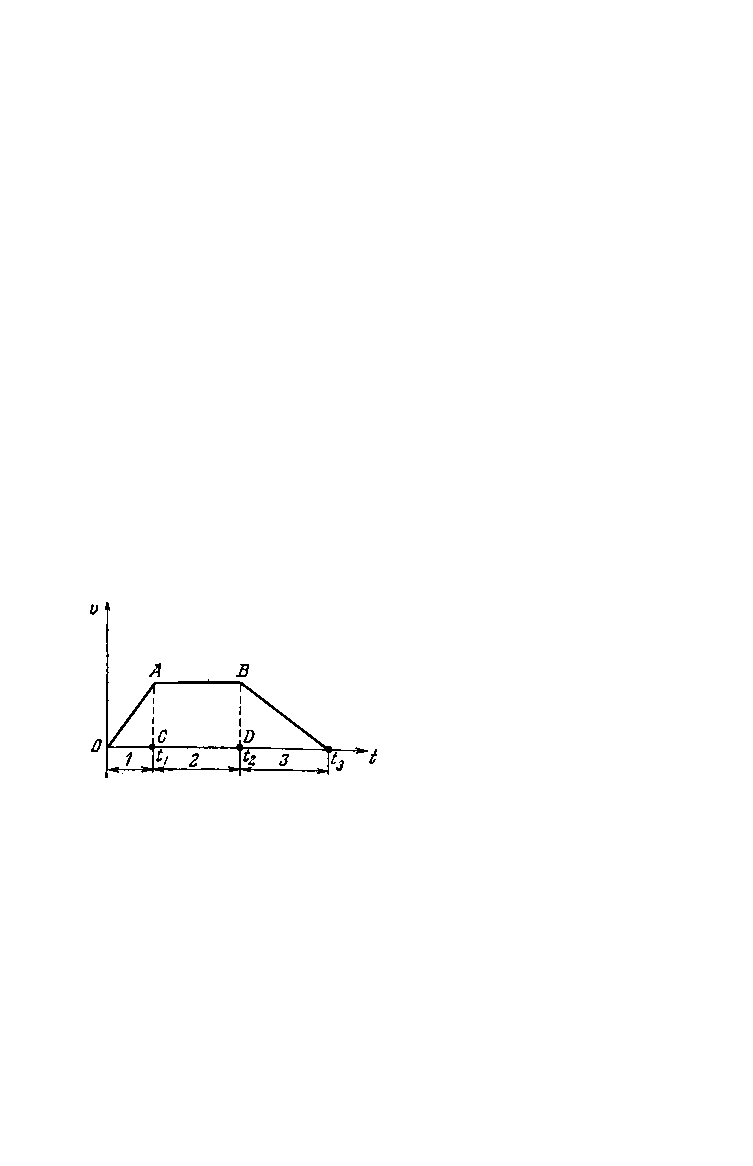
\includegraphics[width=1.1\linewidth]{fig-001.pdf}
\caption{On the basis of this graph can you draw a graph showing the dependence of distance travelled on time.}
\label{fig-01}
\end{marginfigure}

\textsc{Teacher:} Using the velocity graph, can you find the acceleration?\\
\textsc{Student:} Yes. The acceleration is the change in velocity in unit time. It equals the ratio of length $\overline{AC}$ to length $\overline{OC}$.\\
\textsc{Teacher:} Good. Now consider periods 2 and 3.\\
\textsc{Student:} In period 2 the body travels with uniform velocity $v$ acquired at the end of period 1. The formula for the distance travelled is $s=vt$.\\
\textsc{Teacher:} Just a minute, your answer is inaccurate. You have forgotten that the uniform motion began, not at the initial instant of time, but at the instant $t_{1}$. Up to that time, the body had already travelled a distance equal to $\dfrac{at_{1}^{2}}{2}$. The
dependence of the distance travelled on the elapsed time for
period 2 is expressed by the equation
\begin{equation}%
s(t) = \frac{at_{1}^{2}}{2}+ v (t-t_{1})
\label{eq-002}
\end{equation}
With this in mind, please write the formula for the distance travelled in period 3.\\
\textsc{Student:} The motion of the body in period 3 is uniformly decelerated. If I understand it correctly, the formula of the distance travelled in this period should be
$$
s(t) = \frac{at_{1}^{2}}{2}+ v (t_{2}-t_{1}) +  v(t-t_{2}) - \frac{a_{1}(t-t_{2})^2}{2}
$$
where $a_{1}$ is the acceleration in period 3. It is only one half of the acceleration a in period 1, because period 3 is twice as long as period 1.\\
\textsc{Teacher:} Your equation can be simplified somewhat:
\begin{equation}%
s(t) = \frac{at_{1}^{2}}{2}+ v (t-t_{1}) - \frac{a_{1}(t-t_{2})^2}{2}
\label{eq-003}
\end{equation}
Now, it remains to summarize the results of equations \ref{eq-001}, \ref{eq-002} and \ref{eq-003}.\\
\textsc{Student:} I understand. The graph of the distance travelled
has the form of a parabola for period 1, a straight line for period 2 and another parabola
(but turned over, with the convexity facing upward) for period 3. Here is the graph I have drawn (\emph{Figure \ref{fig-02}}).\\
\begin{marginfigure}%
\centering
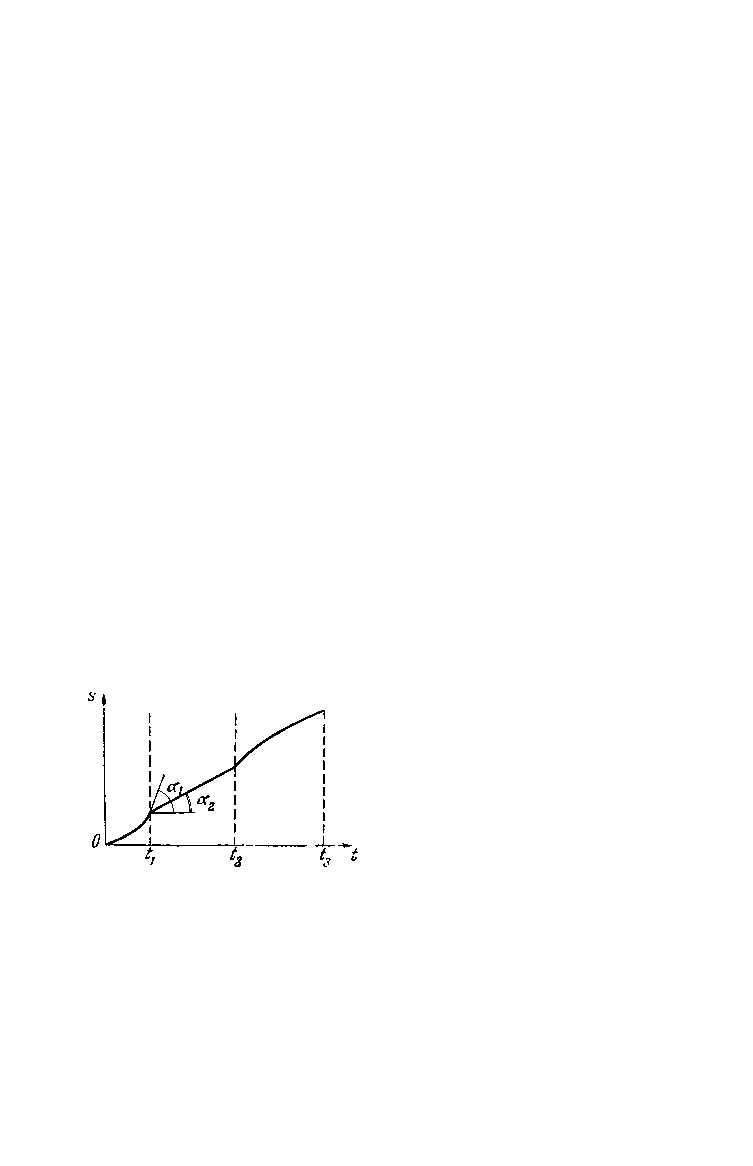
\includegraphics[width=1.1\linewidth]{fig-002.pdf}
\caption{Graph showing distance covered $s$ as a function of time $t$.}
\label{fig-02}
\end{marginfigure}

\textsc{Teacher:} There are two faults in your drawing: the graph of the distance travelled
should have no kinks. It should be a smooth curve, i.e. the parabolas should be tangent to the straight line. Moreover, the vertex of the upper (inverted) parabola should correspond to the instant of time
$t_{3}$. Here is a correct drawing of the graph  (\emph{Figure \ref{fig-03}}).\\

\begin{marginfigure}%
\centering
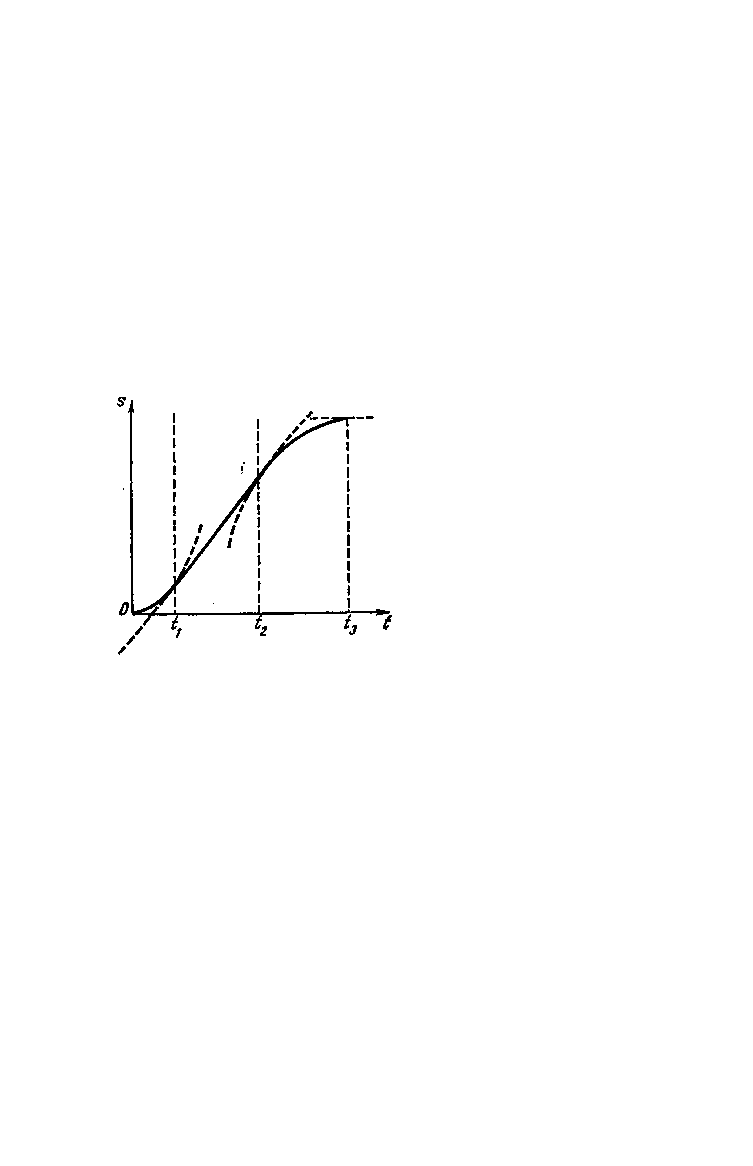
\includegraphics[width=1.1\linewidth]{fig-003a.pdf}
\caption{Corrected graph showing distance covered $s$ as a function of time $t$.}
\label{fig-03}
\end{marginfigure}
\textsc{Student:} Please explain it. \\
\textsc{Teacher:} Let us consider a portion of a distance-travelled \emph{vs} time graph (Fig. 4). The average velocity of the body in the interval from $t$ to $t+\Delta t$ equals 
\begin{equation*}%
\frac{s(t+\Delta t) - s(t)}{\Delta t}= \tan \alpha
\end{equation*}
where $\alpha$ is the angle between chord $AB$ and the horizontal. To determine the velocity of the body at the instant $t$ it is necessary to find the limit of such average velocities for $\Delta t \rightarrow 0$. Thus
\begin{equation}
v(t)=\lim_{\Delta t \rightarrow 0} \frac{s(t+\Delta t)-s(t)}{\Delta t}
\label{eq-004}
\end{equation}

In the limit, the chord becomes a tangent to the distance-travelled \emph{vs} time curve, passing through point $A$ (see the dashed line in \emph{Figure \ref{fig-04}}). The tangent of the angle this line (tangent to the curve) makes with the horizontal is the value of the velocity at the instant $t$. Thus it is possible to find the velocity at any instant of time from the angle of inclination of the tangent to the distance-travelled \emph{vs} time curve at the corresponding point.
\begin{marginfigure}[.5cm]
\centering
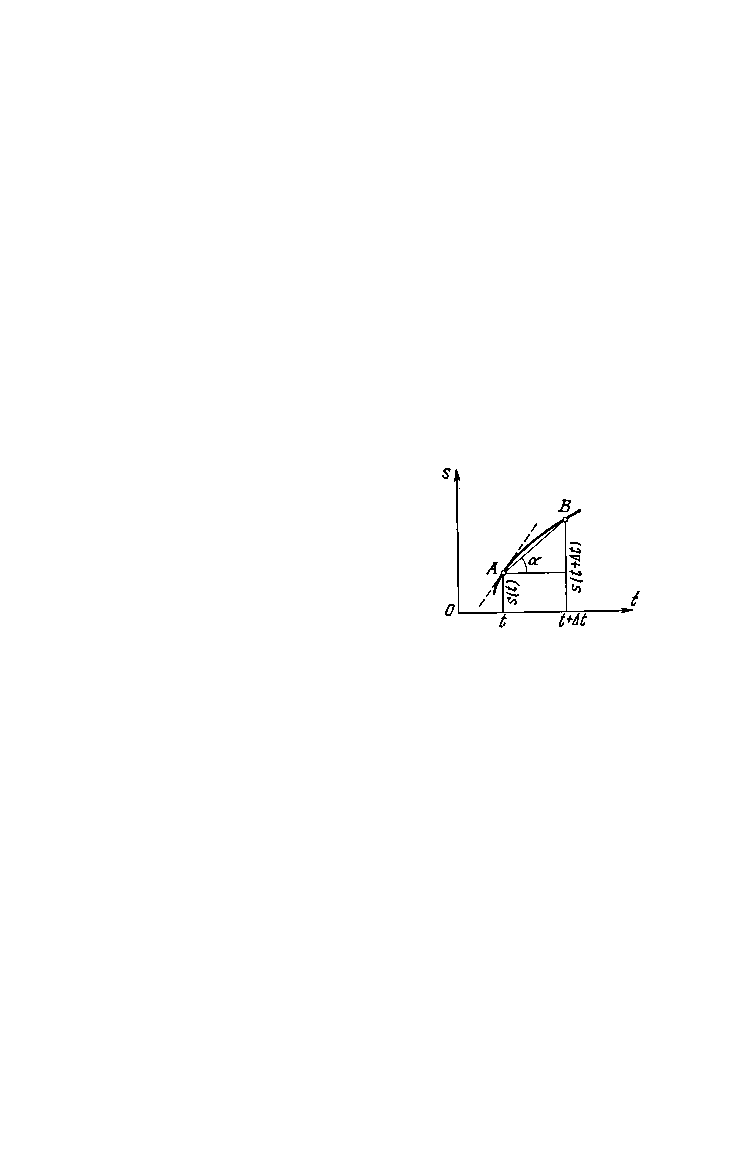
\includegraphics[width=1.1\linewidth]{fig-004a.pdf}
\caption{Corrected graph showing distance covered $s$ as a function of time $t$.}
\label{fig-04}
\end{marginfigure}

But let us return to your drawing (see \emph{Figure \ref{fig-02}}). It follows from your graph that at the instant of time $t_{1}$ (and at $t_{2}$) the velocity of the body has two different values. If we approach $t$, from the left, the velocity equals $\tan \alpha_{1}$, while if we approach it from the right the velocity equals $\tan \alpha_{2}$. According to your graph, the velocity of the body at the instant $t_{1}$ (and again at $t_{2}$) must have a discontinuity, which actually it has not (the velocity \emph{vs} time graph in \emph{Figure \ref{fig-01}} is continuous).\\

\textsc{Student:} I understand now. Continuity of the velocity graph leads to smoothness of the distance-travelled \emph{vs} time graph.\\

\textsc{Teacher:} Incidentally, the vertices of the parabolas should correspond to the instants of time 0 and $t_{3}$ because at these instants the velocity of the body equals zero and the tangent
to the curve must be horizontal for these points. \\
\textit{Now, using the velocity graph in Figure \ref{fig-01}, find the distance travelled by a body by the instant $t_{2}$.} \\
\textsc{Student:} First we determine the acceleration $a$ in period 1 from the velocity graph and then the velocity $v$ in period 2. Next we make use of formula (\ref{eq-002}). The distance travelled by the body during the time $t_{2}$ equals
$$
s(t_{2}) = \frac{at_{1}^{2}}{2}+v(t_{2}-t)
$$
\textsc{Teacher:} Exactly. But there is a simpler way. The distance travelled by the body during the time $t_{2}$ is numerically equal to the area of the figure $OABD$ under the velocity \emph{vs} time graph in the interval $Ot_{2}$. Let us consider another problem to fix what we have learned.\\

\textit{Assume that the distance-travelled \emph{vs} time graph has kinks. This graph is shown in \emph{Figure \ref{fig-05}}, where the curved line is a parabola with its vertex at point $A$. Draw the velocity \emph{vs} timegraph.}
\begin{marginfigure}
\centering
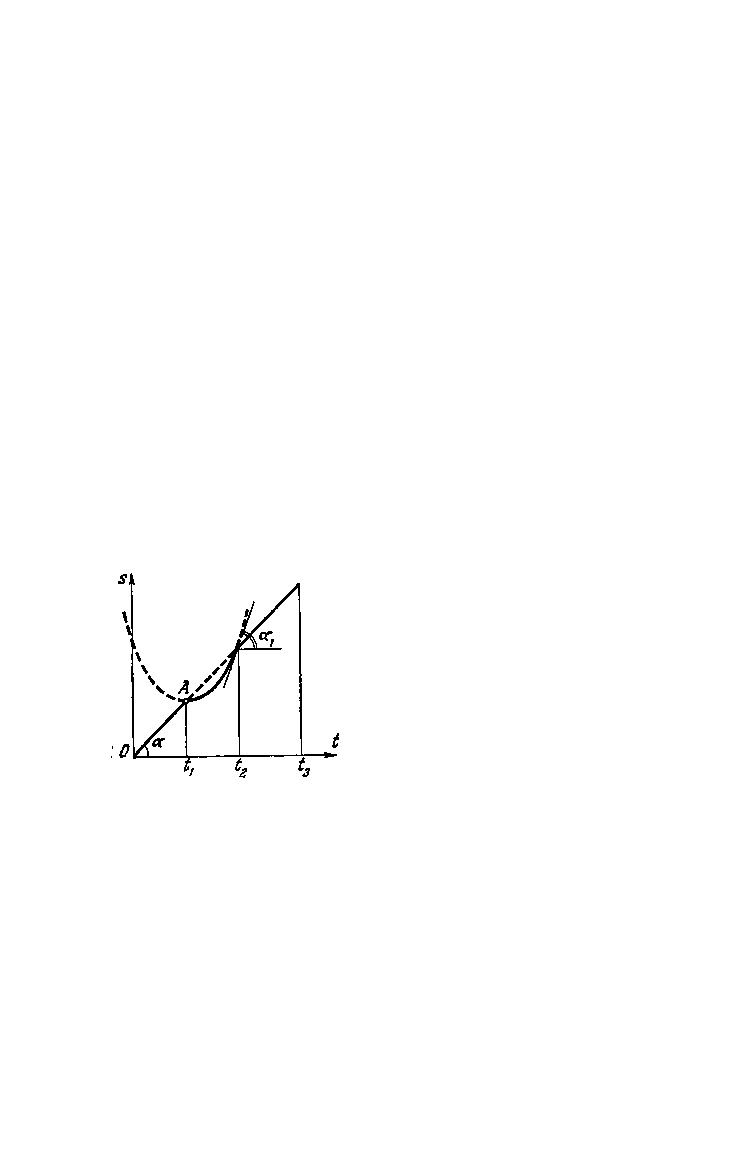
\includegraphics[width=1.1\linewidth]{fig-005a.pdf}
\caption{Corrected graph with kinks showing distance travelled $s$ as a function of time $t$.}
\label{fig-05}
\end{marginfigure}

\textsc{Student:} Since there are kinks in the distance-travelled graph, there should be discontinuities in the velocity graph at the corresponding instants of time ($t_{1}$ and $t_{2}$). Here is my graph (\emph{Figure \ref{fig-06}}).\\

\textsc{Teacher:} Good. What is the length of $\overline{BC}$?\\
\begin{marginfigure}
\centering
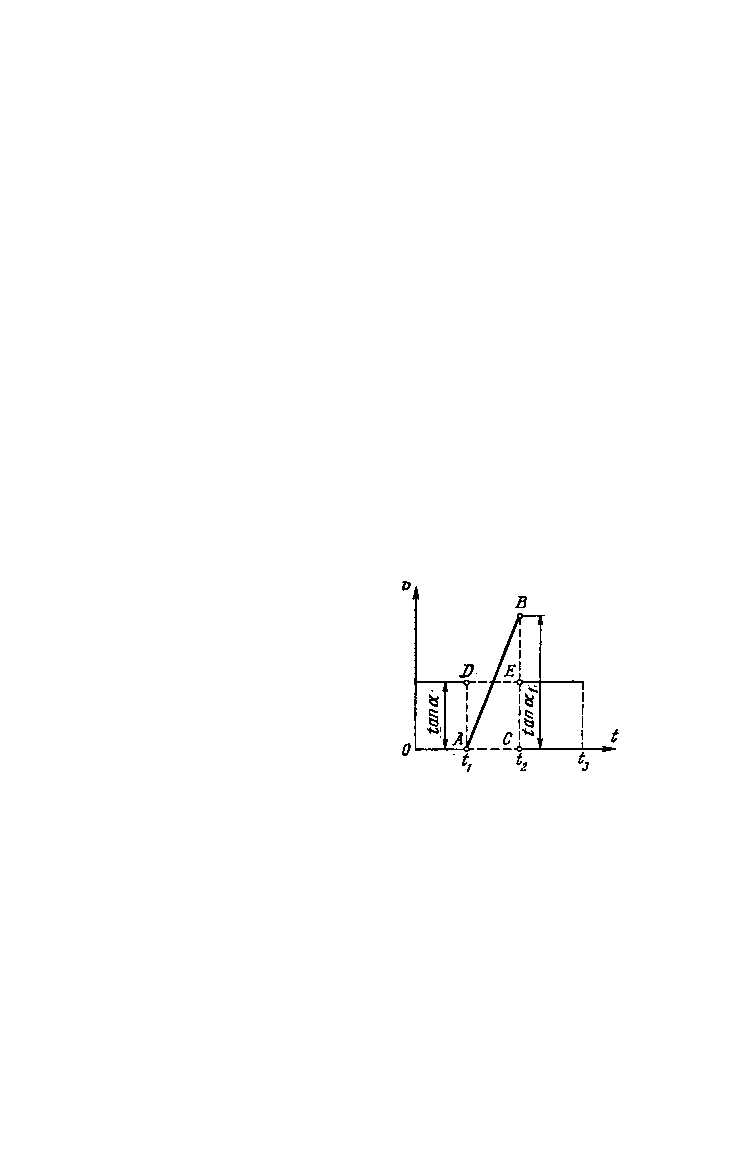
\includegraphics[width=1.1\linewidth]{fig-006a.pdf}
\caption{Velocity \emph{vs} time graph for the function shown in Figure \ref{fig-05}.}
\label{fig-06}
\end{marginfigure}
\textsc{Student:} It is equal to $\tan \alpha_{1}$ (see \emph{Figure \ref{fig-05}}). We don't, however, know the value of angle $\alpha_{1}$.\\
\textsc{Teacher:} Nevertheless, we should have no difficulty in determining the length of $\overline{BC}$. Take notice that the distance travelled by the body by the time $t_{3}$ is the same as if it had travelled at uniform velocity all the time (the straight line in the interval from $t_{2}$ to $t_{3}$ in \emph{Figure \ref{fig-05}} is a continuation of the straight line in the interval from 0 to $t_{1}$). Since the distance travelled is measured by the area under the velocity graph, it follows that the area of rectangle $ADEC$ in \emph{Figure \ref{fig-06}} is equal to the area of triangle $ABC$. Consequently, $BC=2EC$, i.e. the velocity at instant $t_{2}$ when approached from the left is twice the velocity of uniform motion in the intervals from 0 to $t_{1}$ and from $t_{2}$ to $t_{3}$.

\cleardoublepage
\thispagestyle{empty}
\vspace*{2cm}

\begin{figure*}
\centering
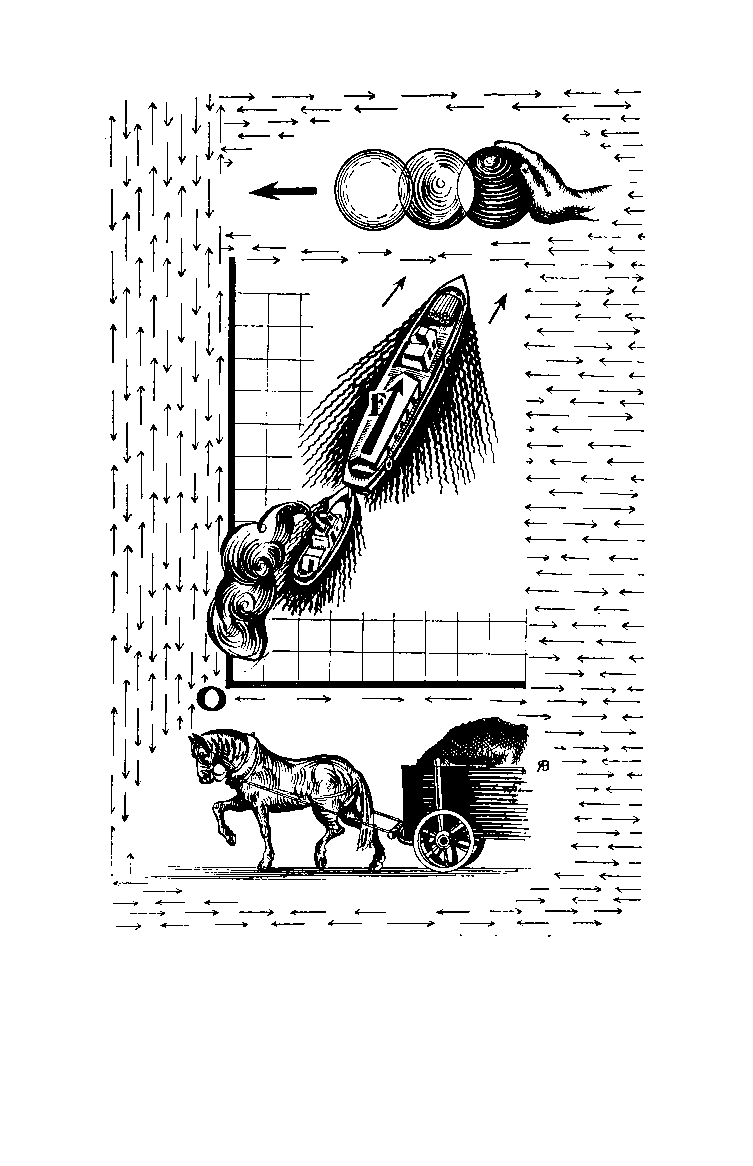
\includegraphics[width=0.7\linewidth]{sec-a.pdf}
\end{figure*}
\begin{centering}
\begin{fullwidth}
%\paragraph{}
{\Large The concept of a force is one of the basic physical concepts. Can you apply it with sufficient facility? Do you have a good understanding of the laws of dynamics?}
\end{fullwidth}
\end{centering}

\chapter{Can You Show The Forces Applied To A Body?}
\label{ch-02}
\paragraph{}
\textsc{Student:} Problems in mechanics seem to be the most difficult of all. How do you begin to solve them?\\

\textsc{Teacher:} Frequently, you can begin by considering the forces applied to a body. As an example, we can take the following cases (Fig. 7): 
\begin{enumerate}[label=(\alph*), leftmargin=*]
\item the body is thrown upward at an angle to the horizontal, 
\item the body slides down an inclined plane, 
\item the body rotates on the end of a string in a vertical plane, and
\item the body is a pendulum.
\end{enumerate}

\begin{marginfigure}
\centering
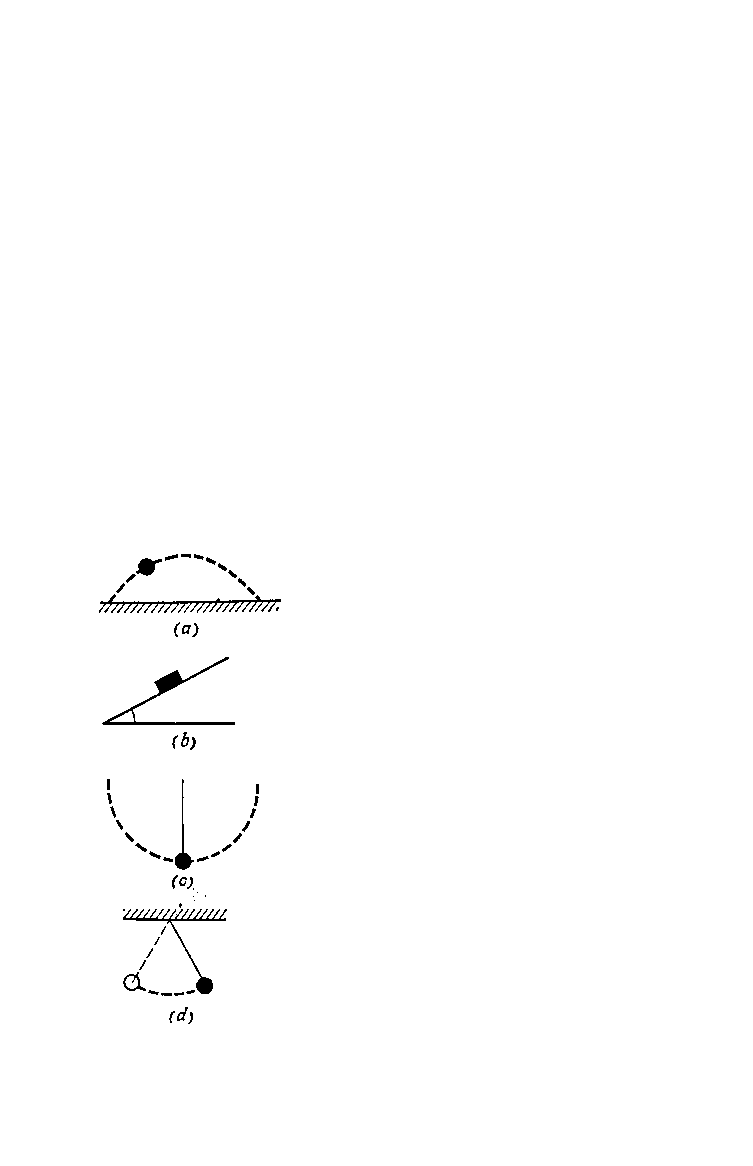
\includegraphics[width=0.7\linewidth]{fig-007a.pdf}
\caption{A variety of different situations for bodies. For each case we have to find out the forces acting on the given body.}
\label{fig-07}
\end{marginfigure}

Draw arrows showing the forces applied to the body in each of these cases, and explain what the arrows represent.\\

\textsc{Student:} Here is my drawing (\emph{Figure \ref{fig-08}}). In the first case, $P$ is the weight of the body and $F$ is the throwing force. In the second, $P$ is the weight, $F$ is the force which keeps the body sliding along the, plane and $F_{fr}$ is the friction force. In the third, $P$ is the weight, $F_{c}$, is the
centripetal force and $T$ is the tension in the string. In the fourth case, $P$ is the weight, $F$ is the restoring force and $T$ is the tension in the string. \\


\textsc{Teacher:} You have made mistakes in all four cases. Here I have the correct drawing (\emph{Figure \ref{fig-09}}). One thing that you must understand clearly is that a force is the result of interaction between bodies. Therefore, to show the forces applied to a body you must first establish what bodies
interact with the given body. Thus, in the first case, only the earth interacts with the body by attracting it (\emph{Figure \ref{fig-09} (a)}). Therefore, only one force, the weight $P$, is applied to the body. If we wished to take into consideration the resistance of the air or, say, the action of the wind, we would have to introduce additional forces. No ``throwing force'', shown in your drawing, actually exists, since there is no interaction creating such a force.\\


\begin{figure}
\centering
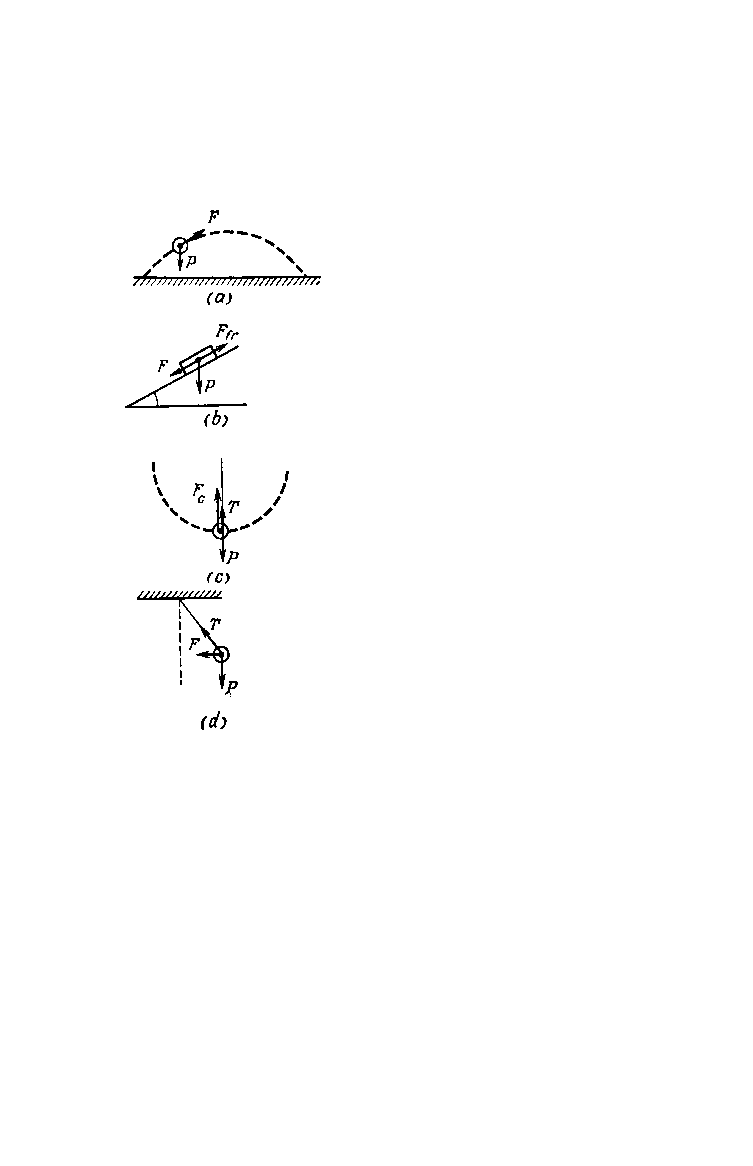
\includegraphics[width=0.4\linewidth]{fig-008a.pdf}
\caption{A variety of different situations for bodies. For each case the student has drawn forces acting on the bodies.}
\label{fig-08}
\end{figure}

\begin{marginfigure}[-8cm]
\centering
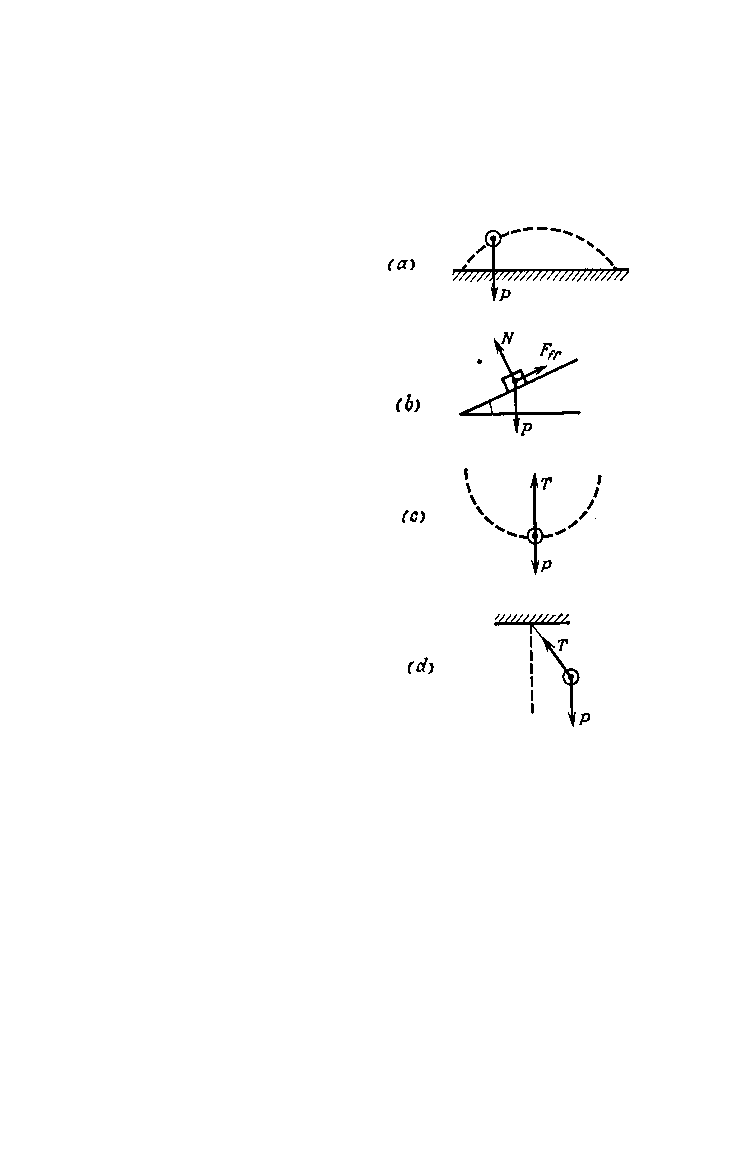
\includegraphics[width=\linewidth]{fig-009a.pdf}
\caption{A variety of different situations for bodies. For each case the correct drawing of forces acting on the bodies are made. Compare this with Figure \ref{fig-08}.}
\label{fig-09}
\end{marginfigure}

\textsc{Student:} But to throw a body, surely some kind of force must be exerted on it.\\

\textsc{Teacher:} Yes, that's true. When you throw a body you exert a certain force on it. In the case above, however, we dealt with the motion of the body after it was thrown, i.e. after the force which imparted a definite initial velocity of flight to the body had ceased to act. It is impossible to ``accumulate'' forces; as soon as the interaction of the bodies ends, the force isn't there any more.\\

\textsc{Student:} But if only the weight is acting on the body, why doesn't it fall vertically downward instead of travelling along a curved path? \\

\textsc{Teacher:} It surprises you that in the given case the direction of motion of the body does not coincide with the direction of the force acting on it. This, however, fully agrees with Newton's second law. Your question shows that you haven't given sufficient thought to Newton's laws of dynamics. I intend to discuss this later (see  Chapter \ref{ch-04}). Now I want to continue our analysis of the four cases of motion of a body. In the second case (\emph{Figure \ref{fig-09}(b)}), a body is sliding down an inclined plane. What bodies are interacting with it?
\\
\textsc{Student:} Evidently, two bodies: the earth and the inclined plane. \\

\textsc{Teacher:} Exactly. This enables us to find the forces applied to the body. The earth is responsible for the weight $P$, and the inclined plane causes the force of sliding friction $F_{fr}$
and the force $N$ ordinarily called the bearing reaction\sidenote{Also called as the normal force}. Note that you entirely omitted force $N$ in your drawing.\\

\textsc{Student:} Just a moment! Then the inclined plane acts on the body with two forces and not one?\\

\textsc{Teacher:} There is, of course, only one force. It is, however, more convenient to deal with it in the form of two component forces, one directed along the inclined plane (force of sliding friction) and the other perpendicular to it (bearing reaction). The fact that these forces have a common origin, i.e, that they are components of the same force, can be seen in the existence
of a universal relation between $F_{fr}$ and $N$:
\begin{equation}
F_{fr}=kN
\label{eq-005}
\end{equation}

where $k$ is a constant called the coefficient of sliding friction. We shall deal with this relationship in more detail later (Chapter \ref{ch-03}). \\

\textsc{Student:} In my drawing, I showed a sliding force which keeps the body sliding down the plane. Evidently, there is no such force. But I clearly remember hearing t.he term ``sliding force'' used frequently in the past. What can you say about this?
 \\
\textsc{Teacher:} Yes, such a term actually exists. You must bear in mind, however, that the sliding force, as you call it, is simply one of the components of the body's weight, obtained when the weight is resolved into two forces, one along the plane and the other normal to it. If, in enumerating the forces applied to the body, you have named the weight, there is no reason to add the sliding force, one of its components. In the third case (\emph{Figure \ref{fig-09}(c)}), the body rotates in a vertical
plane. What bodies act on it?
 \\
\textsc{Student:} Two bodies: the earth and the string. 
\\
\textsc{Teacher:} Good, and that is why two forces are applied to the body: the weight and the tension of the string. 
\\ 
\textsc{Student:} But what about the centripetal force? 
\\
\textsc{Teacher:} Don't be in such a hurry! So many mistakes are made in problems concerning the motion of a body in a circle that I intend to dwell at length on this further on (Chapter \ref{ch-08}).
Here I only wish to note that the centripetal force is not some kind of additional force applied to the body. It is the resultant force. In our case (when the body is at the lowest point of its path), the centripetal force is the difference between the tension of the string and the weight.
\\
\textsc{Student:} If I understand it correctly, the restoring force in the fourth case  (\emph{Figure \ref{fig-09}(d)}) is also the resultant of the tension in the string and the weight? 
\\
\textsc{Teacher:} Quite true. Here, as in the third case, the string and the earth interact with the body. Therefore, two forces, the tension of the string and the weight, are applied to the body.
I wish to emphasize again that forces arise only as a result of interaction of bodies; they cannot originate from any ``accessory'' considerations. Find the bodies acting on the given object and you will reveal the forces applied to the object.
\\
\textsc{Student:} No doubt there are more complicated cases than the ones you have illustrated in  (\emph{Figure \ref{fig-07}}). Can we consider them?
\\
\textsc{Teacher:} There are many examples of more complicated interaction of bodies. For instance, a certain constant horizontal force $F$ acts on a body as a result of which the body moves upward along an inclined surface. The forces applied to the body in this case are shown in  (\emph{Figure \ref{fig-10}}).


\begin{figure}
\centering
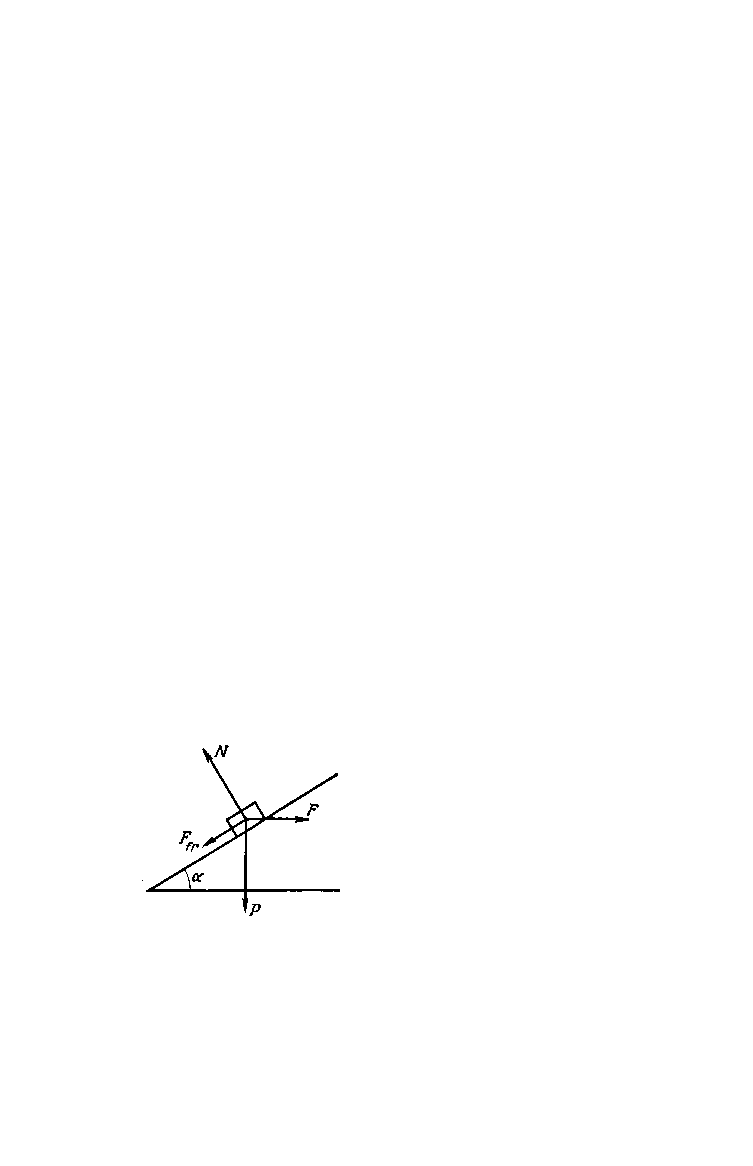
\includegraphics[width=0.4\linewidth]{fig-010a.pdf}
\caption{A variety of different situations for bodies. For each case the student has drawn forces acting on the bodies.}
\label{fig-10}
\end{figure}

Another example is the oscillation of an electrically charged pendulum placed inside a parallel-plate capacitor. Here we have an additional force $F_{e}$ with which the field of the capacitor acts on the charge of the pendulum (\emph{Figure \ref{fig-11}}). It is obviously impossible to mention all the conceivable cases that may come up in solving problems.
\\
\begin{figure}
\centering
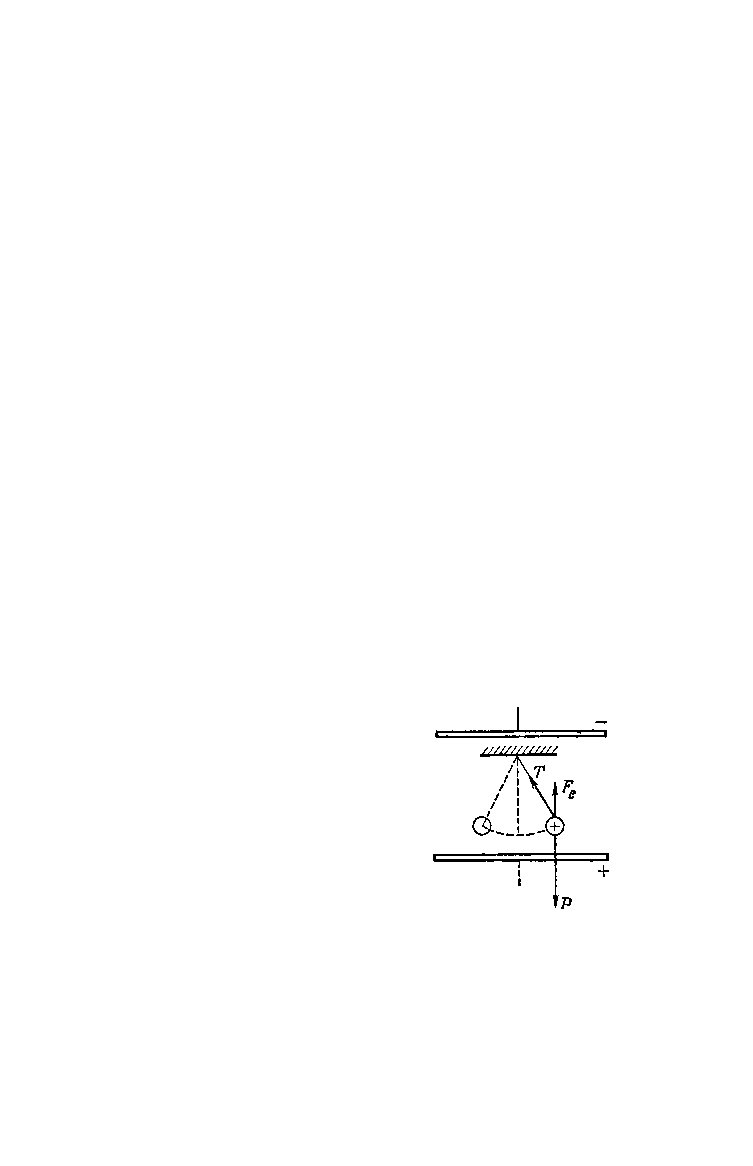
\includegraphics[width=0.4\linewidth]{fig-011a.pdf}
\caption{An electrically charged pendulum inside a parallel plate capacitor.}
\label{fig-11}
\end{figure}
\textsc{Student:} What do you do when there are several bodies in the problem? Take, for example, the case illustrated in \emph{Figure \ref{fig-12}}.
\\
\textsc{Teacher:} You should clearly realize each time the motion of what bodies or combination of bodies you intend to consider. Let us take, for instance, the motion of body 1 in the example you proposed. The earth, the inclined plane and string $AB$ interact with this body.
\\
\begin{figure}
\centering
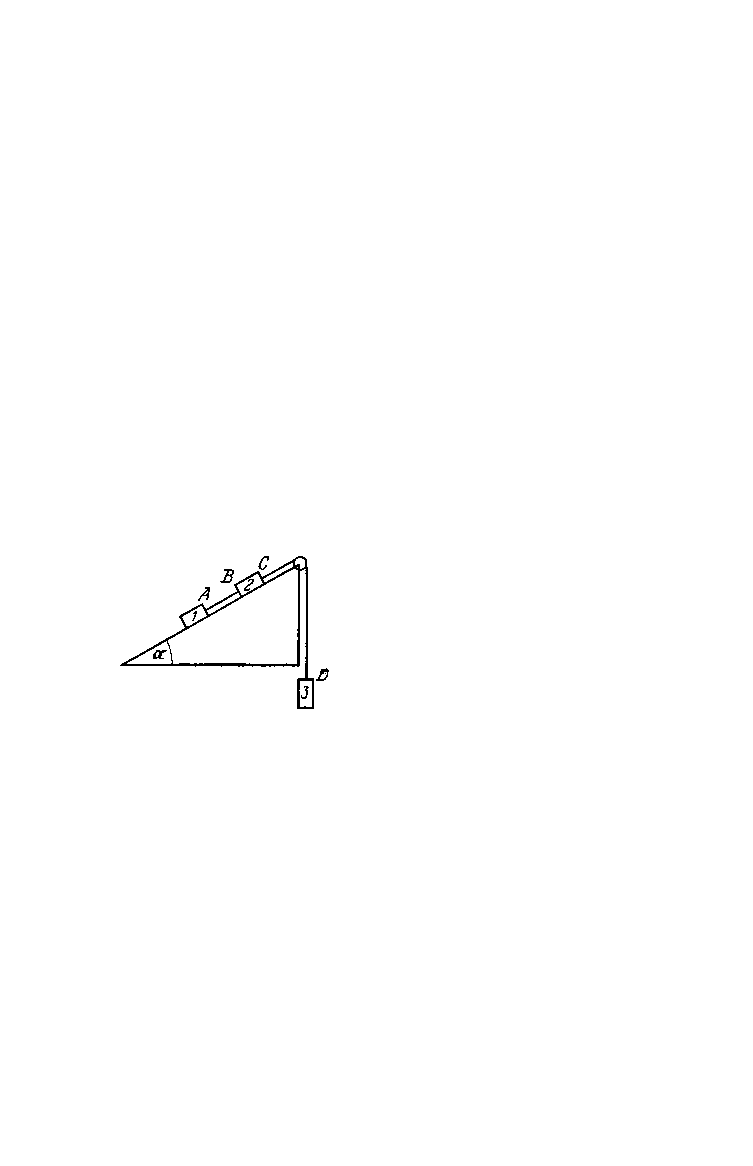
\includegraphics[width=0.4\linewidth]{fig-012a.pdf}
\caption{Three bodies on balanced on a incline.}
\label{fig-12}
\end{figure}

\textsc{Student:} Doesn't body 2 interact with body 1? 
\\
\textsc{Teacher:} Only through string $AB$. The forces applied to body 1 are the weight $P'$,
force $F_{fr}$ of sliding friction, bearing reaction $N'$ and the tension $T'$ of string $AB$ (\emph{Figure \ref{fig-13}(a)}). 
\\
\textsc{Student:} But why is the friction force directed to the left in your drawing? It would seem just as reasonable to have it act in the opposite direction. \\

\begin{figure}
\centering
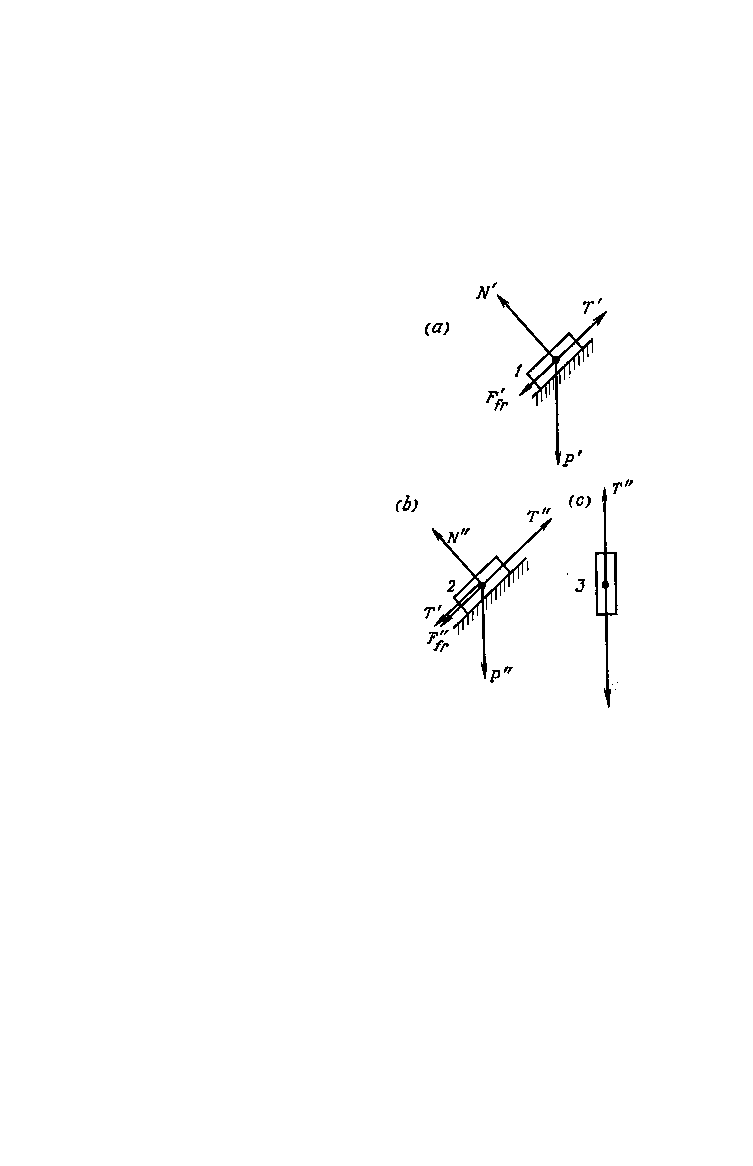
\includegraphics[width=0.5\linewidth]{fig-013a.pdf}
\caption{Forces acting on the three bodies on balanced on a incline shown in Figure \ref{fig-12}.}
\label{fig-13}
\end{figure}

\textsc{Teacher:} To determine the direction of the friction force, it is necessary to know the direction in which the body is travelling. If this has not been specified in the problem, we should assume either one or the other direction. In the given problem, I assume that body 1 (together with the whole
system of bodies) is travelling to the right and the pulley is rotating clockwise. Of course, I cannot know this beforehand; the direction of motion becomes definite only after the corresponding numerical values are substituted. If my assumption is wrong, I shall obtain a negative value when I calculate the acceleration. Then I will have to assume that the body moves to the left instead of to the right (with the pulley rotating counterclockwise) and to direct the force of sliding friction correspondingly. After this I can derive an equation for calculating the acceleration and again check its sign by substituting the numerical values. 
\\
\textsc{Student:} Why check the sign of the acceleration a second time? If it was negative when motion was assumed to be to the right, it will evidently be positive for the second assumption.
\\
\textsc{Teacher:} No, it can turn out to be negative in the second case as well.
\\
\textsc{Student:} I can't understand that. Isn't it obvious that if the body is not moving to the right it must be moving to the left?
\\
\textsc{Teacher:} You forget that the body can also be at rest. We shall return to this question later and analyse in detail the complications that arise when we take the friction force into
consideration (see  Chapter \ref{ch-07}).

For the present, we shall just assume that the pulley rotates clockwise and examine the motion of body 2.
\\
\textsc{Student:} The earth, the inclined plane, string $AB$ and string $CD$ interact with body 2. The forces applied to body 2 are shown in \emph{Figure \ref{fig-13}(b)}.
\\
\textsc{Teacher:} Very well. Now let us go over to body 3.
\\
\textsc{Student:} Body 3 interacts only with the earth and with string $CD$. \emph{Figure \ref{fig-13}(c)} shows the forces applied to body 3.
\\
\textsc{Teacher:} Now, after establishing the forces applied to each body, you can write the equation of motion for each one and then solve the system of equations you obtain.
\\
\textsc{Student:} You mentioned that it was not necessary to deal with each body separately, but that we could also consider the set of bodies as a whole.
\\
\textsc{Teacher:} Why yes; bodies 1, 2 and 3 can be examined, not separately as we have just done, but as a whole. Then, the tensions in the strings need not be taken into consideration since they become, in this case, internal forces, i.e. forces of interaction between separate parts of the item being considered. The system of the three bodies as a whole interacts only with the earth and the inclined plane.
\\
\textsc{Student:} I should like to clear up one point. When I depicted the forces in \emph{Figure \ref{fig-13}(b)} and \emph{(c)}, I assumed that the tension in string $CD$ is the same on both sides of the pulley. Would that be correct?
\\
\textsc{Teacher:} Strictly speaking, that's incorrect. If the pulley is rotating clockwise, the tension in the part of string $CD$ attached to body 3 should be greater than the tension in the part of the string attached to body 2. This difference in tension is what causes accelerated rotation of the pulley. It was
assumed in the given example that the mass of the pulley can be disregarded. In other words, the pulley has no mass that is to be accelerated, it is simply regarded as a means of changing the direction of the string connecting bodies 2 and 3. Therefore, it can be assumed that the tension in string $CD$ is
the same on both sides of the pulley. As a rule, the mass of the pulley is disregarded unless otherwise stipulated. Have we cleared up everything?
\\
\textsc{Student:} I still have a question concerning the point of application of the force. In your drawings you applied all the forces to a single point of the body. Is this correct? Can you apply the force of friction, say, to the centre of gravity of the body?
\\
\textsc{Teacher:} It should be remembered that we are studying the kinematics and dynamics, not of extended bodies, but of material points, or particles, i.e. we regard the body to be of point mass. On the drawings, however, we show a body, and not a point, only for the sake of clarity. Therefore, all the forces can be shown as applied to a single point of the body.
\\
\textsc{Student:} We were taught that any simplification leads to the loss of certain aspects of the problem. Exactly what do we lose when we regard the body as a material point?
\\
\begin{figure}
\centering
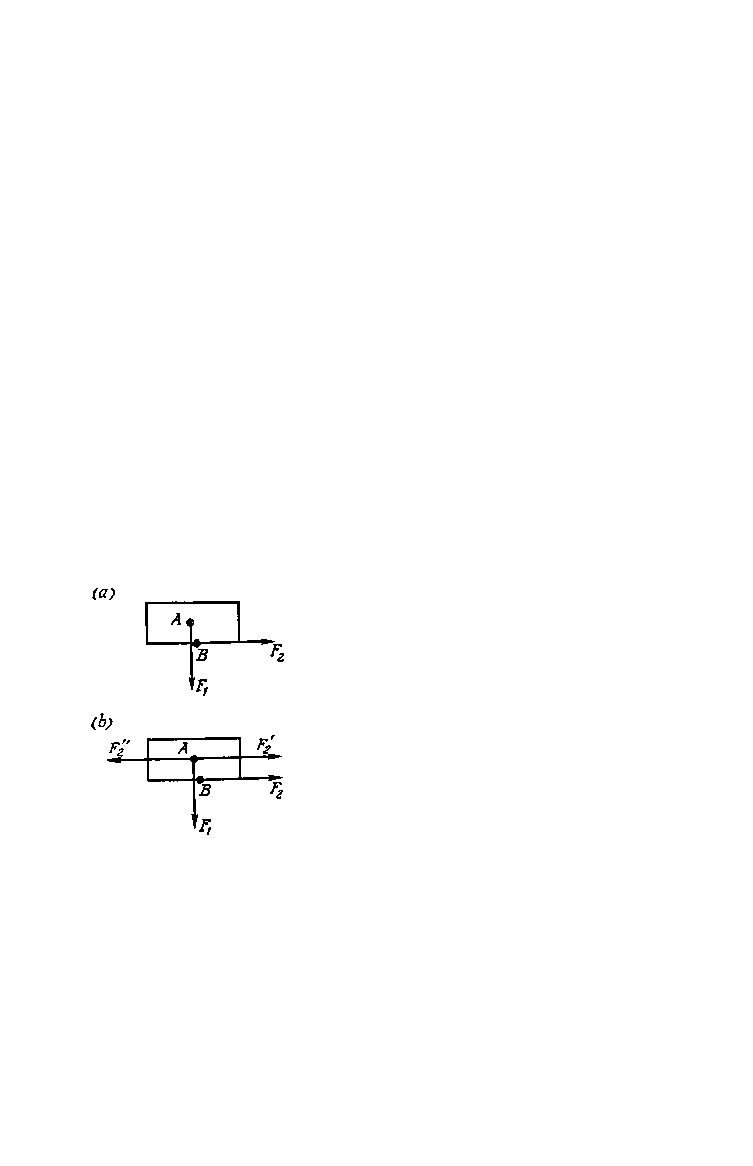
\includegraphics[width=0.4\linewidth]{fig-014a.pdf}
\caption{Forces acting on the three bodies on balanced on a incline shown in Figure \ref{fig-12}.}
\label{fig-14}
\end{figure}
\textsc{Teacher:} In such a simplified approach we do not take into account the rotational moments which, under real conditions, may result in rotation and overturning of the body. A material point has only a motion of translation. Let us consider an example. Assume that two forces are applied at two different points of a body: $F_{1}$ at point $A$ and $F_{2}$ at point $B$, as shown in \emph{Figure \ref{fig-14}(a)}. Now let us apply, at point $A$, force $F_{2}'$  equal and parallel to force $F_{2}$  , and also force $F_{2}''$  equal to force $F_{2}$  but acting in the opposite direction (see \emph{Figure \ref{fig-14}(b)}). Since forces $F_{2}'$ and $F_{2}''$ counterbalance each other, their addition doe! not alter the physical aspect of the problem in any way. However, \emph{Figure \ref{fig-14}(b)} can be interpreted as follows: forces $F_{1}$ and  $F_{2}'$ applied at point $A$ cause motion of translation of
the body also applied to the body is a force couple (forces $F_{2}$ and $F_{2}''$) causing rotation. In other words, force $F_{2}$ can be transferred to point $A$  of the body if, at the same time, the
corresponding rotational moment is added. When we regard the body as a material point, or particle, there will evidently be no rotational moment.\\
\textsc{Student:} You say that a material point cannot rotate but has only motion of translation. But we have already dealt with rotational motion - motion in a circle. \\
\textsc{Teacher:} Do not confuse entirely different things. The motion of translation of a point can take place along various paths, for instance in a circle. When I ruled out the possibility of rotational motion of a point I meant rotation about itself, i.e, about any axis passing through the point.


\chapter{Can You Determine The Friction Force?}
\label{ch-03}

\textsc{Teacher:} I should like to dwell in more detail on the calculation of the friction force in various problems. I have in mind dry sliding friction (sliding friction is said to be dry when there is no layer of any substance, such as a lubricant, between the sliding surfaces).
\\
\textsc{Student:} But here everything seems to be quite clear.
\\
\begin{figure}
\centering
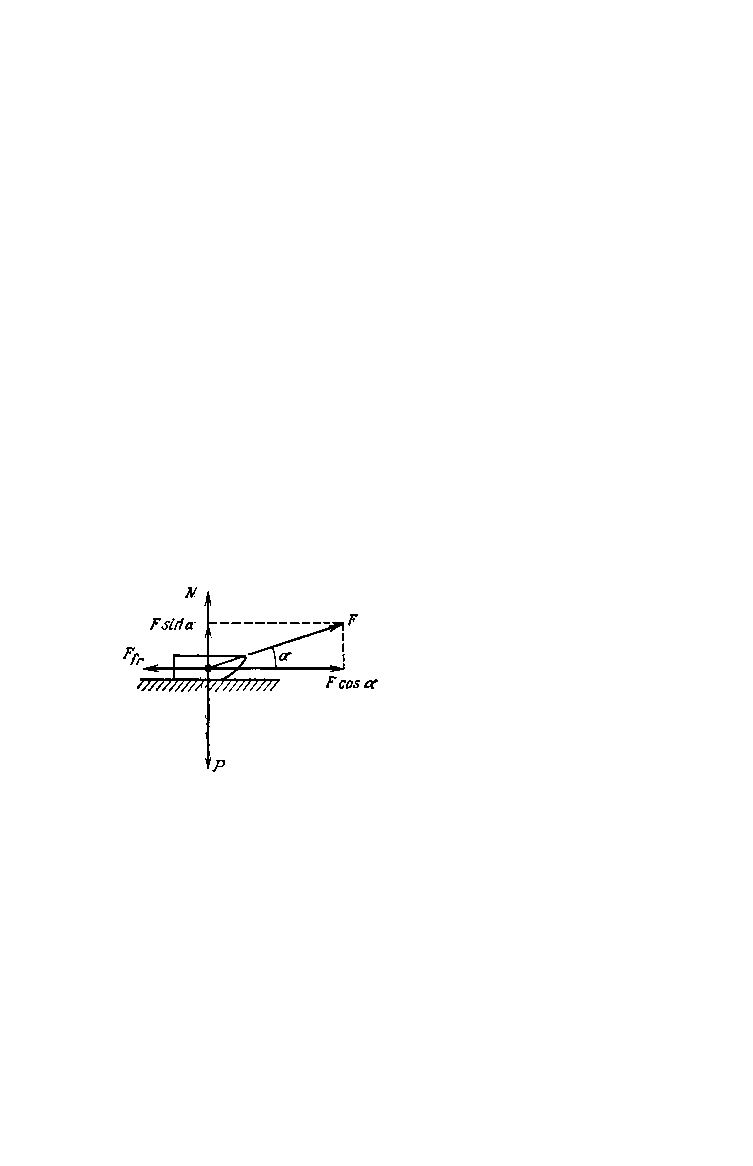
\includegraphics[width=0.55\linewidth]{fig-015a.pdf}
\caption{A sled being pulled with a rope.}
\label{fig-15}
\end{figure}
\textsc{Teacher:} Nevertheless, many mistakes made in examinations are due to the inability to calculate the friction force. Consider the example illustrated in \emph{Figure \ref{fig-15}}. \\

\emph{A sled of weight $P$ is being pulled with a force $F$ applied to a rope which makes an angle $\alpha$ with the horizontal; the coefficient of friction is $k$.}\\
 Find the force of sliding friction. How will you go about it?
\\
\textsc{Student:} Why, that seems to be very simple. The friction force equals $kP$.
\\
\textsc{Teacher:} Entirely wrong. The force of sliding friction is equal, not to $kP$, but to $kN$, where $N$ is the bearing reaction. Remember equation (\ref{eq-005}) from  Chapter \ref{ch-02}.
\\
\textsc{Student:} But isn't that the same thing?
\\
\textsc{Teacher:} In a particular case, the weight and the bearing reaction may be equal to each other, but, in general, they are entirely different forces. Consider the example I proposed. The forces applied to the body (the sled) are the weight $P$, bearing reaction $N$, force $F_{fr}$ of sliding friction and the tension $F$ of the rope (see \emph{Figure \ref{fig-15}}). We resolve force $F$t into its vertical ($F \sin \alpha$) and horizontal ($F \cos \alpha$) components. All forces acting in the vertical direction counterbalance one another. This enables us to find the bearing reaction: 
\begin{equation}
N = P - F \sin \alpha
\label{eq-06}
\end{equation}
As you can see, this force is not equal to the weight of the sled, but is less by the amount $F \sin \alpha$. Physically, this is what should be expected, because the taut rope, being pulled at an angle upwards, seems to ``raise'' the sled somewhat. This reduces the force with which the sled bears on the surface
and thereby the bearing reaction as well. So, in this case, 
\begin{equation}
F_{fr}=k(P - F \sin \alpha)
\label{eq-07}
\end{equation}
If the rope were horizontal ($\alpha=0$), then instead of equation (\ref{eq-06}) we would have $N=P$, from which it follows that $F_{fr}=kP$.
\\
\textsc{Student:} I understand now. I never thought about this before.
\\
\textsc{Teacher:} This is quite a common error of examinees who attempt to treat the force of sliding friction as the product of the coefficient of friction by the weight and not by the bearing reaction. Try to avoid such mistakes in the future.
\\
\textsc{Student:} I shall follow the rule: to find the friction force, first determine the bearing reaction.
\\
\textsc{Teacher:} So far we have been dealing with the force of sliding friction. Now let us consider static friction. This has certain specific features to which students do not always pay
sufficient attention. Take the following example. A body is at rest on a horizontal surface and is acted on by a horizontal force F which tends to move the body. How great do you think the friction force will be in this case?
\\
\textsc{Student:} If the body rests on a horizontal plane and force $F$ acts horizontally, then $N=P$. Is that correct?
\\
\textsc{Teacher:} Quite correct. Continue.
\\
\textsc{Student:} It follows that the friction force equals $kP$.
\begin{figure}
\centering
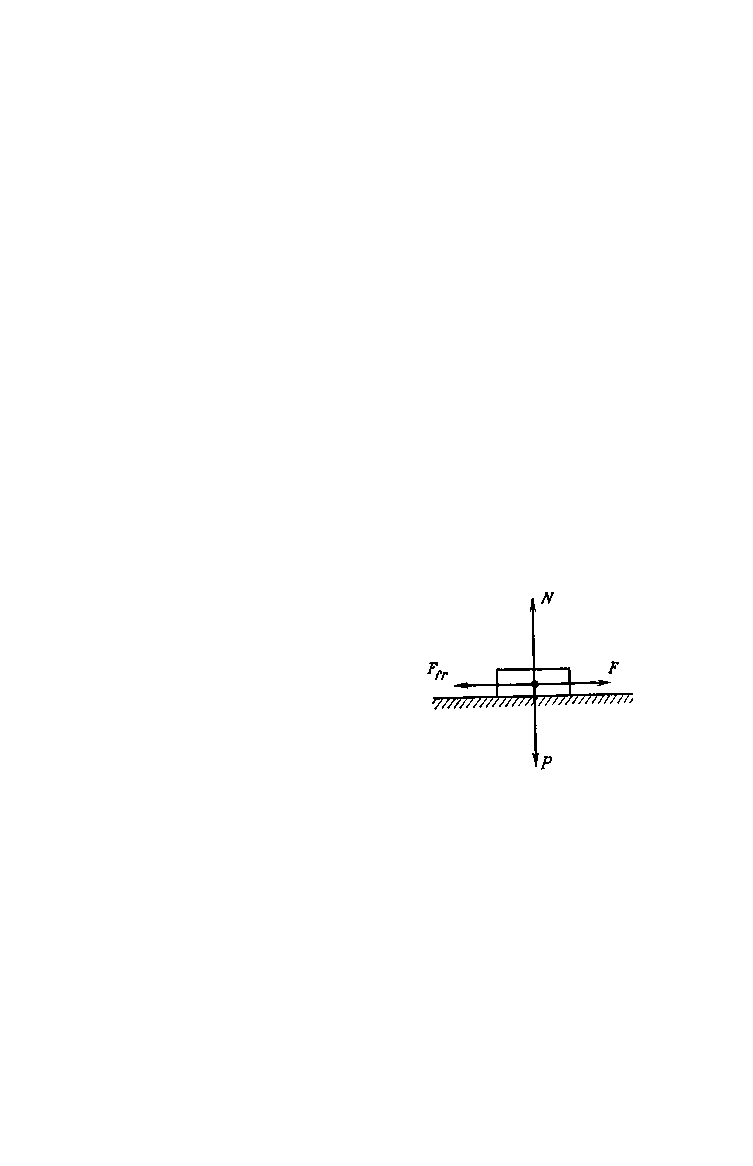
\includegraphics[width=0.55\linewidth]{fig-016a.pdf}
\caption{Forces acting on a body at rest.}
\label{fig-16}
\end{figure}

\textsc{Teacher:} You have made a typical mistake by confusing the forces of sliding and static friction. If the body were sliding along the plane, your answer would be correct. But here the body is at rest. Hence it is necessary that all forces applied to the body counterbalance one another. Four forces act on the body: the weight $P$, bearing reaction $N$, force $F$ and the force of static friction $F_{fr}$ (\emph{Figure \ref{fig-16}}). The vertical forces $P$ and $N$ counterbalance each other. So should the horizontal forces
$F$ and $F_{fr}$ Therefore
\begin{equation}
F_{fr} = F
\label{eq-08}
\end{equation}
\textsc{Student:} It follows that the force of static friction depends on the external force tending to move the body.
\\
\textsc{Teacher:} Yes, that is so. The force of static friction increases with the force F. It does not increase infinitely, however. The force of static friction reaches a maximum value:
\begin{equation}
F_{max} = k_{0}N
\label{eq-09}
\end{equation}


Coefficient $k_{0}$ slightly exceeds coefficient $k$ which characterizes, according to equation (\ref{eq-005}), the force of sliding friction. As soon as the external force F reaches the value $k_{0}N$, the body begins to slide. At this value, coefficient $k_{0}$ becomes equal to $k$, and so the friction force is reduced somewhat. Upon further increase of force $F$, the friction force (now the force of sliding friction) ceases to increase further (until very high velocities are attained), and the body travels with gradually increasing acceleration. The inability of many examinees to determine the friction force is disclosed by the following rather simple question:
 \begin{quote}
 What is the friction force when a body of weight $P$ is at rest on an inclined plane with an angle of inclination $\alpha$?
 \end{quote}
  One hears a variety of incorrect answers. Some say that the friction force equals $kP$, and others that it equals $kN =kP \cos \alpha$.
\\
\textsc{Student:} I understand. Since the body is at rest, we have to deal with the force of static friction. It should be found from the condition of equilibrium of forces acting along the inclined plane. There are two such forces in our case: the friction force $F_{fr}$ and the sliding force $P \sin \alpha$ acting downward along the plane: Therefore, the correct answer is
$$
F_{fr}=P \sin \alpha
$$
\\
\textsc{Teacher:} Exactly. In conclusion, consider the problem illustrated in \emph{Figure \ref{fig-17}}. A load of mass m lies on a body of mass M; the maximum force of static friction between the two is characterized by the coefficient k o and there is no friction between the body and the earth. Find the minimum force F applied to the body at which the load will begin to slide along it.\\
\begin{figure}
\centering
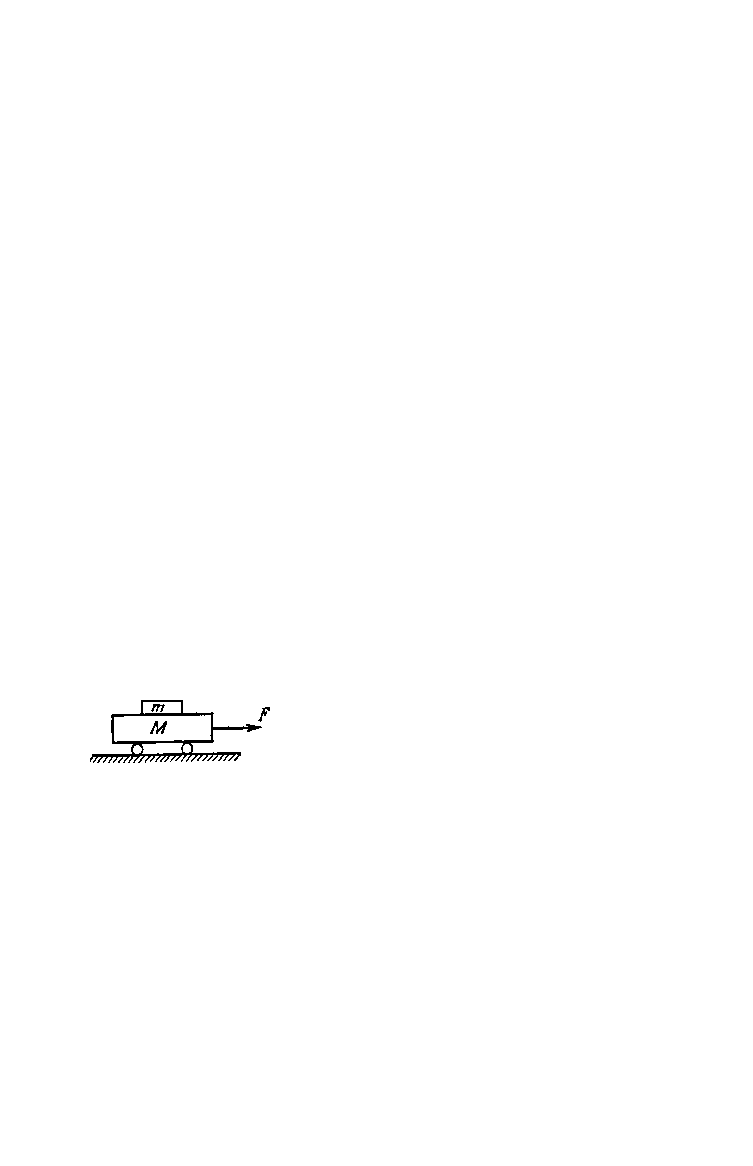
\includegraphics[width=0.55\linewidth]{fig-017a.pdf}
\caption{A load of mass $m$ lies on a body of mass $M$. We have to find the minimum force $F$ so that load begins to slide. }
\label{fig-17}
\end{figure}
\textsc{Student:} First I shall assume that force $F$ is sufficiently small, so that the load will not slide along the body. Then the two bodies will acquire the acceleration \\
$$
a= \frac{F}{M+m}
$$

\textsc{Teacher:} Correct. What force will this acceleration impart to the load?
\\
\textsc{Student:} It will be subjected to the force of static friction $F_{fr}$ by the acceleration. Thus
$$
F_{fr} = ma= \frac{Fm}{M+m}
$$
It follows that with an increase in force $F$, the force of static friction $F_{fr}$ also increases. It cannot, however, increase infinitely. Its maximum value is 
$$
F_{fr \, max}= k_{0}N = k_{0}mg
$$
Consequently, the maximum value of force $F$. at which the two bodies can still travel together as an integral unit is determined from the condition
$$
 k_{0}mg = \frac{Fm}{M+m}
$$
This, then, is the minimum force at which the load begins to slide along the body.
\\
\textsc{Teacher:} Your solution of the proposed problem is correct. I am completely. satisfied with your reasoning.

\chapter{How Well Do You Know Newton's Laws Of Motion?}
\label{ch-04}
\paragraph{}
\textsc{Teacher:} Please state Newton's first law of motion.\\
\textsc{Student:} A body remains at rest or in a state of uniform motion in a straight line until the action of other bodies compels it to change that state. \\
\textsc{Teacher:} Is this law valid in all frames of reference? \\
\textsc{Student:} I don't understand your question. \\
\textsc{Teacher:} If you say that a body is at rest, you mean that it is stationary with respect to some other body which, in the given case, serves as the reference system, or frame of reference. It
is quite pointless to speak of a body being in a state of rest or definite motion without indicating the frame of reference. The nature of the motion of a body depends upon the choice of the frame of reference. For instance, a body lying on the floor of a travelling railway car is at rest with respect to a
frame of reference attached to the car, but is moving with respect to a frame of reference attached to the track. Now we can return to my question. Is Newton's first law valid for all frames of reference?\\
\textsc{Student:} Well, it probably is.\\
\textsc{Teacher:} I see that this question has taken you unawares. Experiments show that Newton's first law is not valid for all reference systems. Consider the example with the body lying
on the floor of the railway car. We shall neglect the friction between the body and the floor. First we shall deal with the position of the body with respect to a frame of reference attached to the car. We can observe the following: the body rests on the floor and, all of a sudden, it begins to slide along the floor even though no action of any kind is evident. Here we have an obvious violation of Newton's first law of motion. The conventional explanation of this effect is that the car, which had been travelling in a straight line and at uniform velocity, begins to slow down, because the train is braked, and the body, due to the absence of friction, continues to maintain its state of uniform straight-line motion with respect to the railway tracks. From this we can conclude that Newton's law holds true in a frame of reference attached to the railway tracks, but not in one attached to a car being slowed down.

Frames of reference for which Newton's first law is valid are said to be inertial; those in which it is not valid are non-inertial. For most of the phenomena we deal with we can assume that any frame of reference is inertial if it is attached to the earth's surface, or to any other bodies which are at rest
with respect to the earth's surface or travel in a straight line at uniform velocity. Non-inertial frames of reference are systems travelling with acceleration (or deceleration), for instance rotating systems, accelerating or decelerating lifts, etc. Note that not only Newton's first law of motion is invalid for non-inertial reference systems, but his second law as well (since the first law is a particular case of the second law).\\
\textsc{Student:} But if Newton's laws cannot be employed for frames of reference travelling with acceleration, then how can we deal with mechanics in such frames?\\
\textsc{Teacher:} Newton's laws of motion can nevertheless be used for non-inertial frames of reference. To do this, however, it will be necessary to apply, purely formally, an additional
force to the body. This force, the so called inertial force, equals the product of the mass of the body by the acceleration of the reference system, and its direction is opposite to the acceleration of the body. I should emphasize that no such force actually exists but, if it is formally introduced, then Newton's laws of motion will hold true in a non-inertial frame of reference.

I want to advise you, however, to employ only inertial frames of reference in solving problems. Then, all the forces that you have to deal with will be really existing forces.\\
\textsc{Student:} But if we limit ourselves to inertial frames of reference, then we cannot analyse, for instance, a problem about a body lying on a rotating disk.\\
\textsc{Teacher:} Why can't we? The choice of the frame of reference is up to you. If in such a problem you use a reference system attached to the disk (i.e, a non-inertial system), the body is considered to be at rest. But if your reference system is attached to the earth (i.e. an inertial reference system), then the body is dealt with as one travelling in a circle.

I would advise you to choose an inertial frame of reference. And now please state Newton's second law of motion.\\
\textsc{Student:} This law can be written as $F=ma$, where $F$ is the
force acting on the body, $m$ is its mass and $a$ the acceleration.\\
\textsc{Teacher:} Your laconic answer is very typical. I should make three critical remarks on your statement; two are not very important and one is essential. In the first place, it is not the force that results from the acceleration, but, on the contrary, the acceleration is the result of the applied force. It is therefore more logical to write the equation of the law as
\begin{equation}
a=\frac{BF}{m}
\label{eq-10}
\end{equation}
where $B$ is the proportionality factor depending upon the choice of units of measurement of the quantities in equation (\ref{eq-10}). Notice that your version had no mention of the proportionality factor $B$. Secondly, a body is accelerated by all forces applied to it (though some may counterbalance one another). Therefore, in stating the law you should use, not the term ``force'', but the
more accurate term ``resultant force''.

My third remark is the most important. Newton's second law establishes a relationship between force and acceleration. But force and acceleration are vector quantities, characterized not only by their numerical value (magnitude) but by their direction as well. Your statement of the law fails to specify
the directions. This is an essential shortcoming. Your statement leaves out a vital part of Newton's second law of motion. Correctly stated it is: the acceleration of a body is directly proportional to the resultant of all forces acting on the body, inversely proportional to the mass of the body and takes place
in the direction of the resultant force. This statement can be analytically expressed by the formula
\begin{equation}
\vec{a}=\frac{B\vec{F}}{m}
\label{eq-11}
\end{equation}
(where the arrows over the letters denote vectors).\\
\textsc{Student:} When in  Chapter \ref{ch-02} we discussed the forces applied to a body thrown upward at an angle to the horizontal, you said you would show later that the direction of motion of a body does not necessarily coincide with the direction of the force applied to it. You referred then to Newton's second law.\\
\begin{figure}
\centering
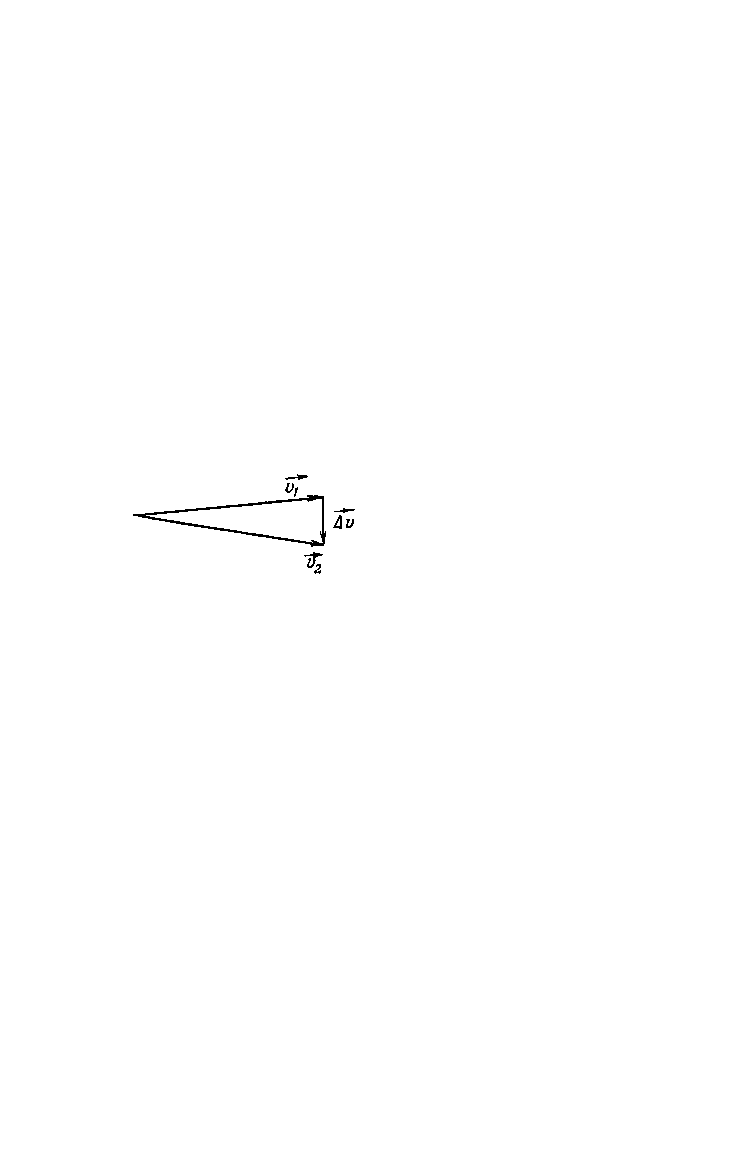
\includegraphics[width=0.55\linewidth]{fig-018a.pdf}
\caption{Depicting change in velocity vectorially.}
\label{fig-18}
\end{figure}
\textsc{Teacher:} Yes, I remember, and I think it would be quite appropriate to return to this question. Let us recall what acceleration is. As we know, acceleration is characterized by the change in velocity in unit time. Illustrated in \emph{Figure \ref{fig-18}} are the velocity vectors $\vec{v_{1}}$ and $\vec{v_{2}}$ of a body for two nearby instants of time $t$ and $t+\Delta t$. The change in velocity during the time $\Delta t$ is the vector $\Delta \vec{v} =\vec{v_{2}} - \vec{v_{1}}$. By definition, the acceleration is
\begin{equation}
\vec{a}(t) \cong \lim_{\Delta t \rightarrow 0}\frac{\Delta \vec{v}}{\Delta t}
\label{eq-12}
\end{equation}
or, more rigorously,
\begin{equation}
\vec{a}(t) = \lim_{\Delta t \rightarrow 0}\frac{\Delta \vec{v}}{\Delta t}
\label{eq-13}
\end{equation}
It follows that the acceleration vector is directed along vector $\Delta v$, which represents the change in velocity during a sufficiently short interval of time. It is evident from \emph{Figure \ref{fig-18}} that the velocity vectors and the change in velocity vector can be oriented in entirely different directions. This means that, in the general case, the acceleration and velocity vectors are also differently oriented. Is that clear?\\
\textsc{Student:} Yes, now I understand. For example, when a body travels in a circle, the velocity of the body is directed along a tangent to the circle, but its acceleration is directed along
a radius toward the centre of rotation (I mean centripetal acceleration).\\
\textsc{Teacher:} Your example is quite appropriate. Now let us return to relationship (equation \ref{eq-11}) and make it clear that it is precisely the acceleration and not the velocity that is oriented
in the direction of the applied force, and that it is again the acceleration and not the velocity that is related to the magnitude of this force. On the other hand, the nature of a body's motion at any given instant is determined by the direction and magnitude of its velocity at the given instant (the velocity vector is always tangent to the path of the body).

Since the acceleration and velocity are different vectors, the direction of the applied force and the direction of motion of the body may not coincide in the general case. Consequently, the nature of the motion of a body at a given instant is not uniquely determined by the forces acting on the body at
the given instant.\\
\textsc{Student:} This is true for the general case. But, of course, the direction of the applied force and the velocity may coincide.\\
\textsc{Teacher:} Certainly, that is possible. Lift a body and release it carefully, so that no initial velocity is imparted to it. Here the direction of motion will coincide with the direction of the force of gravity. If, however, you impart a horizontal initial velocity to the body then its direction of
motion will not coincide with the direction of the gravity force; the body will follow a parabolic path. Though in both cases the body moves due to the action of the same force - its weight - the nature of its motion differs. A physicist would say that this difference is due to the different initial conditions: at
the beginning of the motion the body had no velocity in the first case and a definite horizontal velocity in the second.
\begin{figure}
\centering
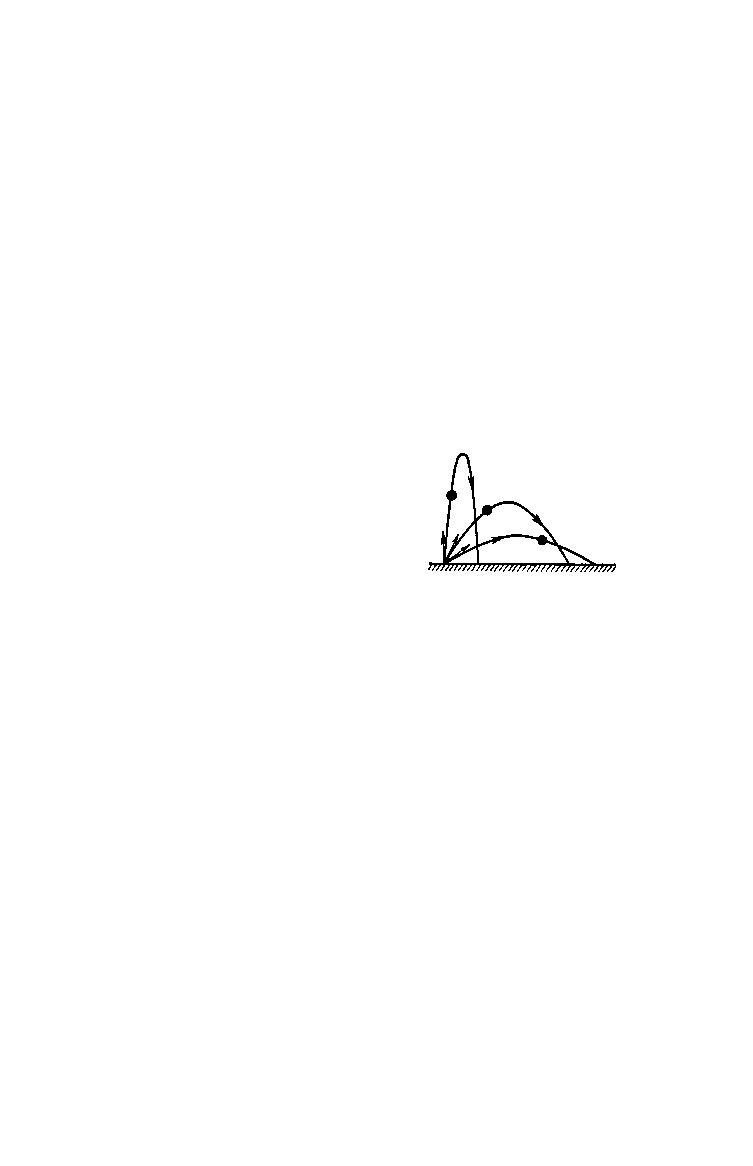
\includegraphics[width=0.55\linewidth]{fig-019a.pdf}
\caption{Trajectories of bodies with different initial velocities.}
\label{fig-19}
\end{figure}

Illustrated in \emph{Figure \ref{fig-19}} are the trajectories of bodies thrown with initial velocities of different directions, but in all cases the same force, the weight of the body, is acting on it.\\
\textsc{Student:} Does that mean that the nature of the motion of a body at a given instant depends not only on the forces acting on the body at this instant, but also on the initial conditions?\\
\textsc{Teacher:} Exactly. It should be emphasized that the initial conditions reflect the prehistory of the body. They are the result of forces that existed in the past. These forces no longer exist, but the result of their action is manifested. From the philosophical. point of view, this demonstrates the relation of the past to the present, i.e, the principle of causality.

Note that if the formula of Newton's second law contained the velocity and not the acceleration, this relationship of the past and present would not be revealed. In this case, the velocity of a body at a given instant (i.e. the nature of its motion at a given instant) would be fully determined by the
forces acting on the body precisely at this instant; the past would have no effect whatsoever on the present.

I want to cite one more example illustrating the aforesaid. It is shown in \emph{Figure \ref{fig-20}}: a ball hanging on a string is subject to the action of two forces, the weight and the tension of the string. If it is deflected to one side of the equilibrium position and then released, it will begin to oscillate. If, however, a definite velocity is imparted to the ball in a direction perpendicular to the plane of deviation, the ball will begin to travel in a circle at uniform velocity. As you can see, depending upon the initial conditions, the ball either oscillates in a plane (see \emph{Figure \ref{fig-20}(a)}), or travels at uniform velocity in a circle (see \emph{Figure \ref{fig-20}(b)}. Only two forces act on it in either case: its weight and the tension of the string.
\\
\begin{marginfigure}
\centering
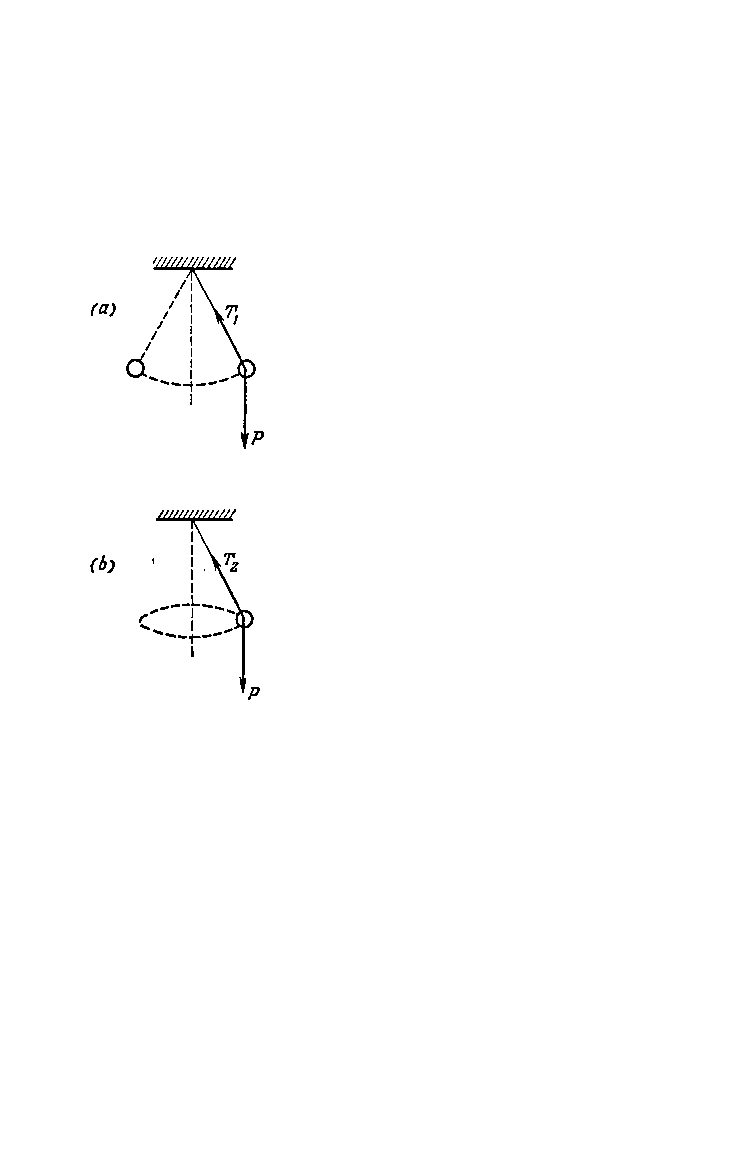
\includegraphics[width=0.7\linewidth]{fig-020a.pdf}
\caption{A ball hanging from a string can have different resultant motions depending on the initial conditions.}
\label{fig-20}
\end{marginfigure}
\textsc{Student:} I haven't considered Newton's laws from this viewpoint.
\\
\textsc{Teacher:} No wonder then that some students, in trying to determine the forces applied to a body, base their reasoning on the nature of motion without first finding out what bodies interact with the given body. You may recall that you did the same. That is exactly why, when drawing \emph{Figures \ref{fig-08}(c)} and \emph{\ref{fig-08}(d)}, it seemed to you that the sets of forces applied to the body in those cases should be different. Actually, in both cases two forces are applied to the body: its weight and the tension of the string.
\\
\textsc{Student:} Now I understand that the same set of forces can cause motions of different nature and therefore data on the nature of the motion of a body cannot serve as a starting point in determining the forces applied to the body.
\\
\textsc{Teacher:} You have stated the matter very precisely. There is no need, however, to go to the extremes. Though different kinds of motion may be caused by the same set of forces (as
in \emph{Figure \ref{fig-20}}), the numerical relations between the acting forces differ for the different kinds of motion. This means that there will be a different resultant applied force for each motion. Thus, for instance, in uniform motion of a body in a circle, the resultant force should be the centripetal one; in oscillation in a plane, the resultant force should be the restoring force. From this it follows that even though data on the kind of motion of a body cannot serve as the basis for determining the applied forces, they are far from superfluous.

In this connection, let us return to the example illustrated in Fig. 20. Assume that the angle ex, between the vertical and the direction of the string is known and so is the weight $P$ of the body. Find the tension $T$ in the string when 
\begin{enumerate}[label=\Roman*]
\item  the oscillating body is in its extreme position, and
\item when the body is travelling uniformly in a circle.
\end{enumerate}

In the first case, the resultant force is the restoring force and it is perpendicular to the string. Therefore, the weight $P$ of the body is resolved into two components, with one component along the
resultant force and the other perpendicular to it (i.e. directed along the string). Then the forces
perpendicular to the resultant force, i. e. those acting in the direction along the string, are equated to each other (see \emph{Figure \ref{fig-21}(a)}). Thus
$$
T_{1} = P \cos \alpha
$$

\begin{figure}
\centering
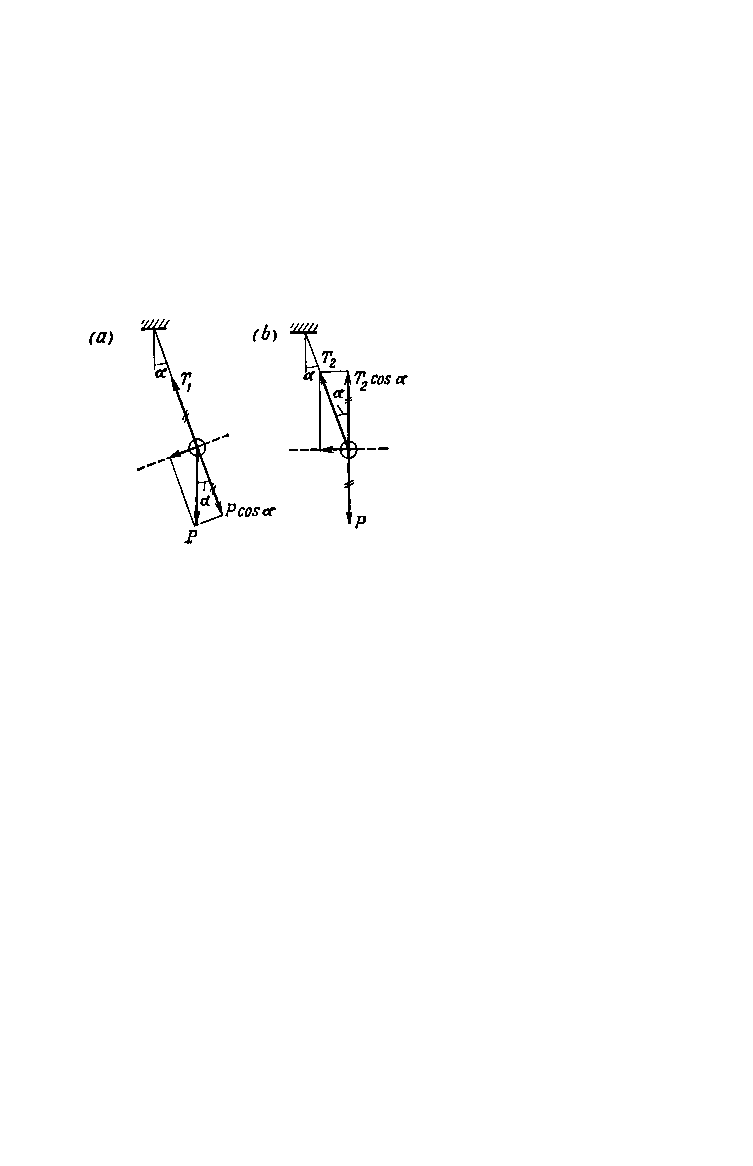
\includegraphics[width=0.7\linewidth]{fig-021a.pdf}
\caption{Resolving the forces on a moving pendulum.}
\label{fig-21}
\end{figure}

In the second case, the resultant force is the centripetal one and is directed horizontally. Hence, the
tension $T_{2}$ of the string should be resolved into a vertical and a horizontal force, and the forces perpendicular to the resultant force, i.e, the vertical forces, should be equated to each other (\emph{Figure \ref{fig-21}(b)}). 

Then
$$
T_{2} \cos \alpha = P \quad \text{or} \quad T_{2} = \frac{P}{\cos \alpha}
$$
As you can see, a knowledge of the nature of the body's motion proved useful in finding the tension of the string.
\\
\textsc{Student:} If I understand all this correctly, then, knowing the interaction of bodies, you can find the forces applied to one of them; if you know these forces and the initial conditions, you can predict the nature of the motion of the body (the magnitude and direction of its velocity at any instant).
On the other hand, if you know the kind of motion of a body you can establish the relationships between the forces applied to it. Am I reasoning correctly?
\\
\textsc{Teacher:} Quite so. But let us continue. I want to propose a comparatively simple problem relating to Newton's second law is caused by the resultant of all the forces applied to it. 
\\
There are four such forces and their resultant is $F-f$. This is what causes the acceleration of the system. Now you see that this acceleration is not associated with the interaction between the horse and the waggon.
\\
\textsc{Student:} So the earth's surface turns out to be, not simply the place on which certain events occur, but an active participant of these events.
\\
\textsc{Teacher:} Your pictorial comment is quite true. Incidentally, if you locate the horse and waggon on an ideal icy surface, thereby excluding all horizontal interaction between this system and the earth, there will be no motion, whatsoever. It should be stressed that no internal interaction can impart acceleration to a system as a whole. This can be done only by external action (you can't lift yourself by your hair, or bootstraps either). This is an important practical inference of Newton's third law of motion.
%\newpage
\cleardoublepage
\thispagestyle{empty}
\vspace*{2cm}
\begin{centering}

\begin{figure*}
\centering

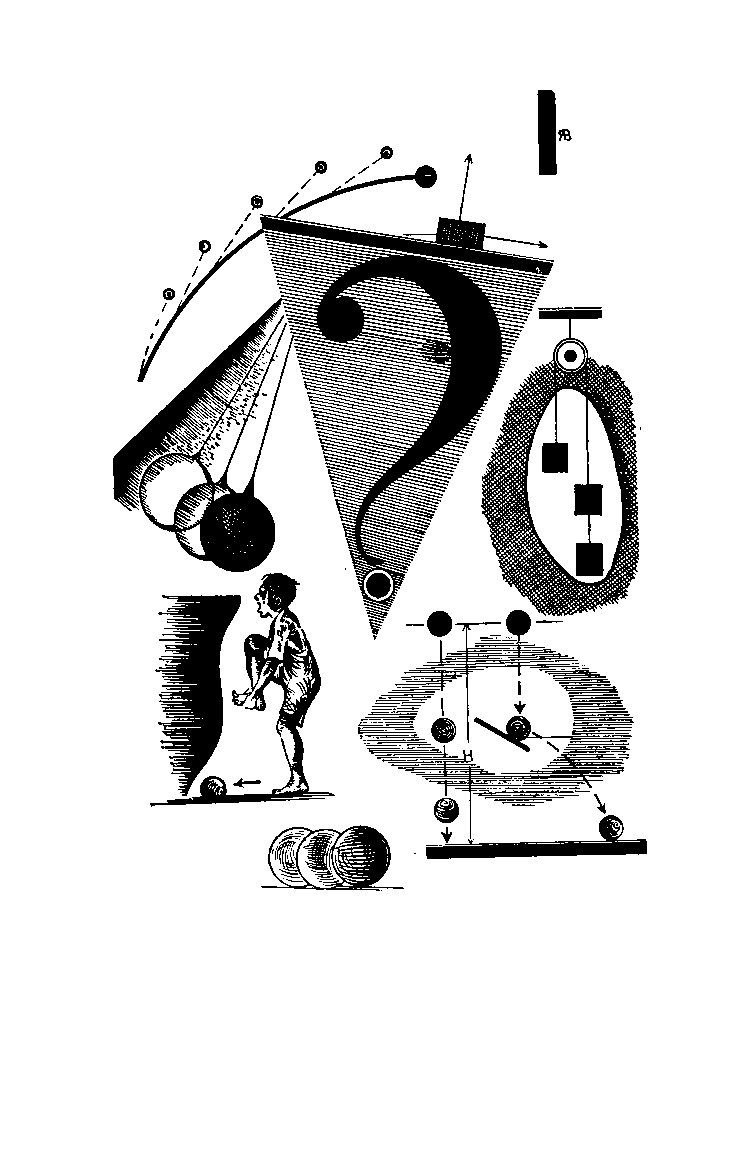
\includegraphics[width=0.7\linewidth]{sec-b.pdf}
%\caption{Velocity \emph{vs} time graph for the function shown in Figure \ref{fig-05}.}
%\label{fig-06}
\end{figure*}
 \addtocounter{figure}{1}
% For incrementing the figure numbers for figures without caption or numbering
\begin{fullwidth}
\begin{Large}
%\paragraph{}
If you know mechanics well, you can easily solve problems. The converse is just as true: if you solve problems readily, you evidently have a good knowledge of mechanics. Therefore, extend your knowledge of mechanics by solving as many problems as you can.
\end{Large}
\end{fullwidth}
\end{centering}


\chapter{How Do You Go About Solving Problems In Kinematics?}
\label{ch-05}
\paragraph{}
\textsc{Teacher:} Assume that two bodies are falling from a certain height. One has no initial velocity and the other has a certain initial velocity in a horizontal direction. Here and further on
we shall disregard the resistance of the air. Compare the time it takes for the two bodies to fall
to the ground.\\
\textsc{Student:} The motion of a body thrown horizontally can be regarded as a combination of two motions: vertical and horizontal. The time of flight is determined by the vertical component of the
motion. Since the vertical motions of the bodies are determined in both cases by the same data (same height and the absence of a vertical component of the initial velocity), the time of fall is the same for the two bodies. \\
It equals $\sqrt{\dfrac{2H}{g}}$, where $H$ is the initial height.\\
\textsc{Teacher:} Absolutely right. Now let us consider a more complex case. Assume that both bodies are falling from the height $H$ with no initial velocity, but in its path one of them meets a fixed plane, inclined at an angle of \ang{45} to the horizontal. As a result of this impact on the plane the direction of the velocity of the body becomes horizontal (\emph{Figure \ref{fig-23}}). The point of impact is at the height $h$. Compare the times of fall of the two bodies.
\\
\begin{figure}
\centering
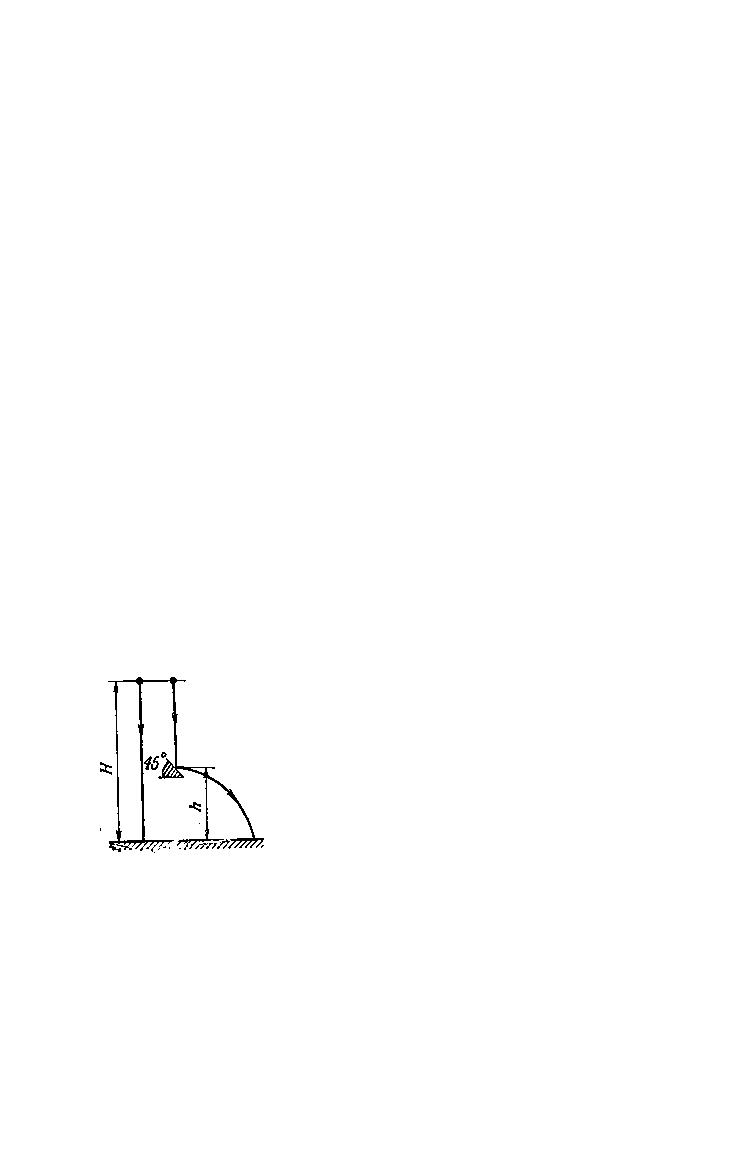
\includegraphics[angle=-1.2,width=0.4\linewidth]{fig-023a.pdf}
\caption{Two bodies falling from height $H$. One of them meets a fixed plane at height $h$. Problem is to compare the time of fall of the two bodies.}
\label{fig-23}
\end{figure}
\textsc{Student:} Both bodies take the same time to fall to the level of the inclined
plane. As a result of the impact on the, plane one of the bodies acquires a horizontal component of velocity. This horizontal component cannot, however, influence the vertical component of the body's motion. Therefore, it follows that in this case as well the time of fall should be the same for the bodies.
\\
\textsc{Teacher:} Your answer is wrong. You were right in saying that the horizontal component of the velocity doesn't influence the vertical motion of the body and, consequently, its time of
fall. When the body strikes the inclined plane it not only acquires a horizontal velocity component, but also loses the vertical component of its velocity, and this of course must affect the time of fall. After striking the inclined plane, the body falls from the height $h$ with no initial vertical velocity. The impact against the plane delays the vertical motion of the body and thereby increases its time of fall. The time of fall for the body which dropped straight to the ground is $\sqrt{\dfrac{2H}{g}}$; that for the body striking the plane is 
$$
\sqrt{\frac{2 (H-h)}{g}}+\sqrt{\frac{2h}{g}}
$$
This leads us to the following question: \emph{at what $h$ to $H$ ratio will the time of fall reach its maximum value?} In other words, at what height should the inclined plane be located so that it delays the fall most effectively?
\\
\textsc{Student:} I am at a loss to give you an exact answer. It seems to me that the ratio $\dfrac{h}{H}$ should not be near to 1 or to 0, because a ratio of 1 or 0 is equivalent to the absence of any
plane whatsoever. The inclined plane should be located somewhere in the middle between the ground and the initial point.
\\
\textsc{Teacher:} Your qualitative remarks are quite true. But you should find no difficulty in obtaining the exact answer. We can write the time of fall of the body as
$$
t = \sqrt{\frac{2 H}{g}} \left( \sqrt{1-x} + \sqrt{x} \right) \, \, \text{where} \, \, x = \frac{h}{H}
$$
Now we find the value of $x$ at which the function $t(x)$ is a maximum. First we square the time of fall. Thus
$$
t^{2} = \frac{2 H}{g} \left(  1 +2\sqrt{(1-x) x}  \right)
$$
If the time is maximal, its square is also maximal. It is evident from the last equation that t 2 is a maximum when the function $y= (1- x) x$ is a maximum. Thus, the problem is reduced to finding the maximum of the quadratic trinomial 
$$
y = -x^{2} + x = - \left( x- \frac{1}{2}\right)^2 + \frac{1}{4}
$$
This trinomial is maximal at $x= \dfrac{1}{2}$. Thus, height $h$ should be one half of height $H$.

Our further discussion on typical procedure for solving problems in kinematics will centre around the example of a body thrown upward at an angle to the horizontal (usually called the elevation angle).
\\
\textsc{Student:} I'm not very good at such problems.
\\
\textsc{Teacher:} We shall begin with the usual formulation of the problem: \emph{a body is thrown upward at an angle of $\alpha$, to the horizon with: an initial velocity of $v_{0}$. Find the time of flight $T$, maximum height reached $H$ and the range $L$.} 

As usual, we first find the forces acting on the body. The only force is gravity. Consequently, the body travels at uniform velocity in the horizontal direction and with uniform acceleration $g$ in the vertical direction. We are going to deal with the vertical and horizontal components of motion separately, for which purpose we resolve the initial velocity vector into the vertical ($v_{0} \sin \alpha$,) and horizontal ($v_{0} \cos \alpha$,) components. The horizontal velocity component remains constant throughout the flight while the vertical component varies as shown in \emph{Figure \ref{fig-24}}. \\
\begin{figure}
\centering
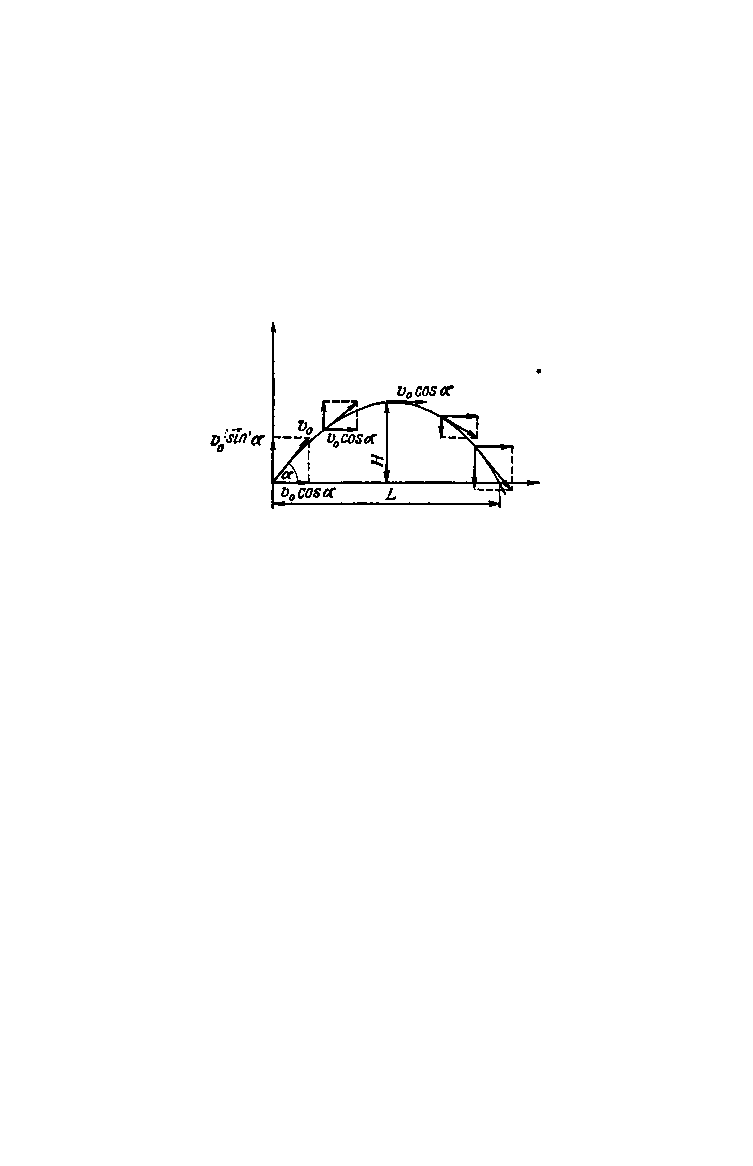
\includegraphics[width=0.7\linewidth]{fig-024a.pdf}
\caption{A body thrown with an angle $\alpha$ to the horizon. The problem is to find the time of flight, maximum height reached and the range of the body.}
\label{fig-24}
\end{figure}


Let us examine the vertical component of the motion. The time of flight $T= T_{1} +T_{2}$, where $T_{1}$ is the time of ascent (the body travels vertically with uniformly decelerated motion) and $T_{2}$ is the time of descent (the body travels vertically downward with uniformly accelerated motion). The vertical
velocity of the body at the highest point of its trajectory (at the instant $t=T_{1}$) is obviously equal to zero. On the other hand, this velocity can be expressed by the formula showing the dependence of the velocity of uniformly decelerated motion on time. Thus we obtain
$$
0 = v_{0} \sin \alpha - gT_{1}
$$
or
\begin{equation}
T_{1} = \frac{v_{0} \sin \alpha}{g}
\label{eq-14}
\end{equation}

When $T_{1}$ is known we can obtain
\begin{equation}
H = v_{0} T_{1} \sin \alpha -  \frac{v_{0}^{2} \sin^{2} \alpha}{g}
\label{eq-15}
\end{equation}

The time of descent $T_{2}$ can be calculated as the time a body falls from the known height H without any initial vertical velocity:
$$
T_{2} = \sqrt{\frac{2H}{g}} = \frac{v_{0} \sin \alpha}{g}
$$

Comparing this with equation (\ref{eq-14}) we see that the time of
descent is equal to the time of ascent. The total time of flight is
\begin{equation}
T= \frac{2 v_{0} \sin \alpha}{g}
\label{eq-16}
\end{equation}

To find the range $L$, or horizontal distance travelled, we make use of the horizontal component of motion. As mentioned before, the body travels horizontally at uniform velocity. Thus
\begin{equation}
L= (v_{0} \cos \alpha) T = \frac{v_{0}^{2} \sin 2 \alpha}{g}
\label{eq-17}
\end{equation}

It can be seen from equation (\ref{eq-17}) that if the sum of the angles at which two bodies are thrown is \ang{90} and if the initial velocities are equal, the bodies will fall at the same point. Is everything clear to you so far?
\\
\textsc{Student:} Why yes, everything seems to be clear.
\\
\textsc{Teacher:} Fine. Then we shall add some complications. \emph{Assume that a horizontal tail wind of constant force $F$ acts on the body. The weight of the body is $P$. Find, as in. the
preceding case, the time of flight $T$, maximum height reached $H$, and range $L$.}\\

\textsc{Student:} In contrast to the preceding problem, the horizontal motion of the body is not uniform; now it travels with a horizontal acceleration of 
$$
a= \left( \frac{F}{P} \right)g
$$
\textsc{Teacher:} Have there been any changes in the vertical component of motion?
\\
\textsc{Student:} Since the force of the wind acts horizontally the wind cannot affect the vertical motion of the body.
\\
\textsc{Teacher:} Good. Now tell me which of the sought for quantities should have the same values as in the preceding problem.
\\
\textsc{Student:} These will evidently be the time of flight $T$ and the height $H$. They are the ones determined on the basis of the vertical motion of the body. They will therefore be the same as in the preceding problem.
\\
\textsc{Teacher:} Excellent. How about the range?
\\
\textsc{Student:} The horizontal acceleration and time of flight being known, the range can be readily found. Thus
$$
L  = \left( v_{0} \cos \alpha \right)T + \frac{aT^{2}}{2} = \frac{v_{0}^{2} \sin 2 \alpha}{g} + \frac{2F}{P}\frac{v_{0}^{2} \sin^{2} \alpha}{g}
$$
\\
\textsc{Teacher:} Quite correct. Only the answer would best be written in another form:
\begin{equation}
L= (v_{0} \cos \alpha) T = \frac{v_{0}^{2} \sin 2 \alpha}{g}
\label{eq-18}
\end{equation}
Next we shall consider a new problem: \emph{a body is thrown at an angle $\alpha$ to an inclined plane which makes the angle $\beta$ with the horizontal (\emph{Figure \ref{fig-25}}). The body's initial velocity is $v_{0}$. Find the distance $L$ from the point where the body is thrown to the point where it falls on the plane.}
\\
\begin{figure}
\centering
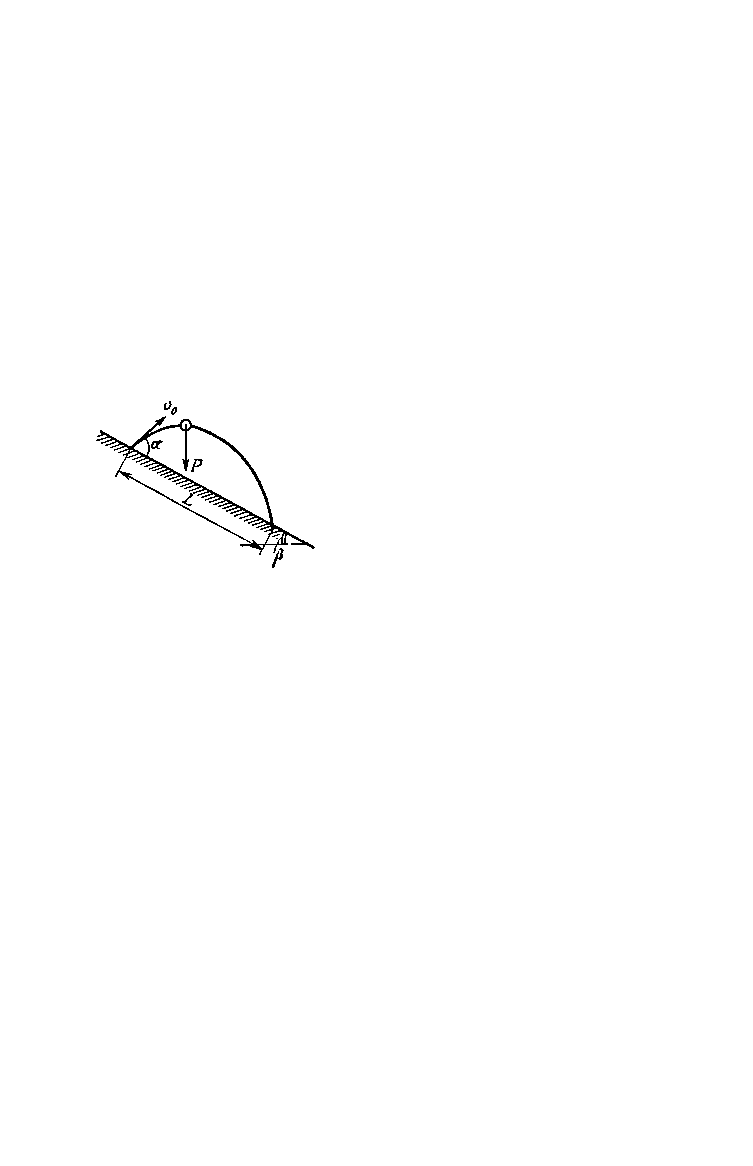
\includegraphics[width=0.6\linewidth]{fig-025a.pdf}
\caption{A body thrown with an angle $\alpha$ to the horizon. The problem is to find the time of flight, maximum height reached and the range of the body.}
\label{fig-25}
\end{figure}
\textsc{Student:} I once made an attempt to solve such a problem but failed.
\\
\textsc{Teacher:} Can't you see any similarity between this problem and the preceding one?
\\
\textsc{Student:} No, I can't.
\\
\textsc{Teacher:} Let us imagine that the figure for this problem
is turned through the angle $\beta$ so that the inclined plane becomes horizontal (\emph{Figure \ref{fig-26}(a)}).

\begin{figure*}
\centering
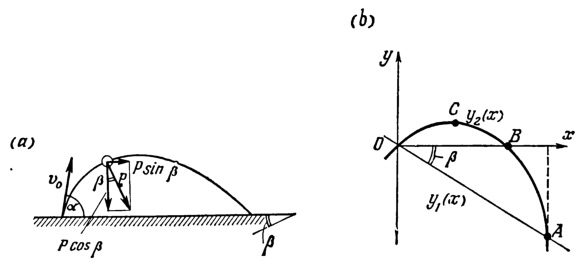
\includegraphics[width=0.8\linewidth]{fig-026a.pdf}
\caption{Rotating the Figure \ref{fig-25} through angle $\beta$ gives us a problem similar to the one we have solved in the previous section. }
\label{fig-26}
\end{figure*}

Then the force of gravity is no longer vertical. Now we resolve it into a vertical ($P \cos \beta$) and
a horizontal ($P \sin \beta$) component. You can readily see now that we have the preceding problem again, in which the force $P \sin \beta$ plays the role of the force of the wind, and $P \cos \beta$ the role of the force of gravity. Therefore we can find the answer by making use of equation (\ref{eq-18}) provided that we make the following substitutions:
$$
P \sin \beta \, \, \text{for} \, \, F, P \cos \beta \, \, \text{for} \, \, P, \, \, \text{and} \, \, g \cos \beta \, \, \text{for} \, \, g
$$
Then we obtain
\begin{equation}
L= \frac{v_{0}^{2} \sin 2 \alpha}{g \cos \beta } \left( 1 + \tan \beta tan \alpha \right)
\label{eq-19}
\end{equation}
At $\beta =0$, this coincides with equation (\ref{eq-17}). 

Of interest is another method of solving the same problem. We introduce the coordinate axes $Ox$ and $Oy$ with the origin at the point the body is thrown from (\emph{Figure \ref{fig-26}(b)}). The inclined plane is represented in these coordinates by the linear function
$$
y_{1}=-x \tan \beta
$$
and the trajectory of the body is described by the parabola
$$
y_{2}= ax^{2}+bx
$$
in which the factors $a$ and $b$ can be expressed in terms of $v_{0}$, $\alpha$ and $\beta$. Next we find the coordinate $x_{A}$ of the point $A$ of intersection of functions $y_{1}$ and $y_{2}$ by equating the expressions for these functions
$$
- x \tan \beta = ax^{2} + bx
$$
From this it follows that 
$$
x_{A} = \left( \frac{\tan \beta+b}{-a} \right)
$$
Then we can easily find the required distance 
\begin{equation}
L= \frac{x_{A}}{\cos \beta } = \frac{ \tan \beta + b} {a \cos \beta}
\label{eq-20}
\end{equation}
It remains to express factors $a$ and $b$ in terms of $v_{0}$, $\alpha$ and $\beta$. For this purpose, we examine two points of the parabola - $B$ and $C$ (see \emph{Figure \ref{fig-26}(b)}). We write the equation of the parabola for each of these points:
\begin{equation*}
\left.
\begin{aligned}
 y_{2C} &= ax^{2}_{C} + bx_{C} \\
y_{2B} &= ax^{2}_{B} + bx_{B}
\end{aligned}
\right\}
\end{equation*}

%\begin{equation*} |x| =
%\begin{cases} 
%x & \text{if $x\ge 0$}\\ 
%-x & \text{if $x\le 0$}
%\end{cases} 
%\end{equation*}
The coordinates of points $C$ and $B$ are known to us. Consequently, the preceding system of equations enables us to determine factors $a$ and $b$. I suggest that in your spare time you complete
the solution of this problem and obtain the answer in the form of equation (\ref{eq-19}).
\\
\textsc{Student:} I like the first solution better.
\\
\textsc{Teacher:} That is a matter of taste. The two methods of solution differ essentially in their nature. The first could be called the ``physical'' method. It employs simulation which is so typical of the physical approach (we slightly altered the point of view and reduced our problem to the previously
discussed problem with the tail wind). The second method could be called ``mathematical''. Here we employed two functions and found the coordinates of their points of intersection.

In my opinion, the first method is the more elegant, but less general. The field of application of the second method is substantially wider. It can, for instance, be applied in principle when the profile of the hill from which the body is thrown is not a straight line. Here, instead of the linear function $y_{1}$, some other function will be used which conforms to the profile of the hill. The first method is inapplicable in principle in such cases. We may note that the more extensive field of application of mathematical methods is due to their more abstract nature.

\section{PROBLEMS}
\label{problems-01}
%\begin{fullwidth}
\begin{enumerate}[series=problems]
\item Body $A$ is thrown vertically upward with a velocity of \SI[per-mode=symbol]{20}{\meter \per \second}. At what height was body $B$ which, when thrown at a horizontal velocity of  \SI[per-mode=symbol]{4}{\meter \per \second} at the same time body $A$ was thrown, collided with it in its
flight? The horizontal distance between the initial points of the flight equals \SI{4}{m}. Find also the time of flight of each body before the collision and the velocity of each at the instant of collision.
\item From points $A$ and $B$, at the respective heights of \SIlist{2;6}{\metre}, two bodies are thrown simultaneously towards each other: one is thrown horizontally with a velocity of \SI[per-mode=symbol]{8}{\meter \per \second} and the other, downward at an angle of \ang{45} to the horizontal and at an initial velocity such that the bodies collide in flight. The horizontal distance between points $A$ and $B$ equals \SI{8}{m}. Calculate the initial velocity $v_{0}$ of the body thrown at an angle of \ang{45}, the coordinates $x$ and $y$ of the point of collision, the time of flight t of the bodies before colliding and the velocities $v_{A}$ and $v_{B}$ of the two bodies at the instant of collision. The trajectories of the bodies lie in a single plane.
\item Two bodies are thrown from a single point at the angles $\alpha_{1}$ and $\alpha_{2}$ to the horizontal and at the initial velocities $v_{1}$ and $v_{2}$, respectively. At what distance from each other will the bodies be after the time $t$? Consider two cases: 
\begin{enumerate}[label=(\arabic*)]
\item the trajectories of the two bodies lie in a single plane and the bodies are thrown in opposite directions, and 
\item the trajectories lie in mutually perpendicular planes.
\end{enumerate}
\item A body falls from the height $H$ with no initial velocity. At the height $h$ it elastically bounces off a plane inclined at an angle of \ang{30} to the horizontal. Find the time it takes the body to reach the ground.
\item At what angle to the horizontal (elevation angle) should a body of weight $P$ be thrown so that the maximum height reached is equal to the range? Assume that a horizontal tail wind of constant force $F$ acts on the body in its flight.
\item A stone is thrown upward, perpendicular to an inclined plane with an angle of inclination $\alpha$. If the initial velocity is $v_{0}$, at what distance from the point from which it is thrown will the stone fall?

\item A boy \SI{1.5}{m} tall, standing at a distance of \SI{15}{m} from a fence \SI{5}{m}
high, throws a stone at an angle of \ang{45} to the horizontal. With what minimum velocity should the stone be thrown to fly over the fence?
\end{enumerate}
%\end{fullwidth}


\chapter{How Do You Go About Solving Problems In Dynamics?}
\label{ch-06}
\paragraph{}
\textsc{Teacher:} In solving problems in dynamics it is especially important to be able to determine correctly the forces applied to the body (see Chapter \ref{ch-02}).
\\
\textsc{Student:} Before we go any further, I wish to ask one question. Assuming that I have correctly found all the forces applied to the body, what should I do next?
\\
\textsc{Teacher:} If the forces are not directed along a single straight line, they should be resolved in two mutually perpendicular directions. The force components should be dealt with separately for each of these directions, which we shall call ``directions of resolution''. We can begin with some practical advice. In the first place, the forces should be drawn in large scale to avoid confusion in resolving them. In trying to save space students usually represent forces in the form of almost microscopic arrows, and this does not help. You will understand what I mean if you compare your drawing (\emph{Figure \ref{fig-08}}) with mine (\emph{Figure \ref{fig-09}}). Secondly, do not hurry to resolve the forces before it can be done properly. First you should find all forces applied to the body, and show them in the drawing. Only then can you begin to resolve some of them. Thirdly, you must remember that after you have resolved a force you should ``forget'' about its existence and use only its components. Either the force itself, or its components, no compromise.
\\
\textsc{Student:} How do I choose the directions of resolution?
\\
\textsc{Teacher:} In making your choice you should consider the nature of the motion of the body. There are two alternatives:
\begin{enumerate}[label=(\arabic*)]
\item the body is at rest or travels with uniform velocity in a straight line, and 
\item the body travels with acceleration and the direction of acceleration is given (at least its sign).
\end{enumerate}

In the first case you can select the directions of resolution arbitrarily, basing (or not basing) your choice on considerations of practical convenience. Assume, for instance, that in the case illustrated in \emph{Figure \ref{fig-10}} the body slides with uniform velocity up the inclined plane. Here the directions of resolution may be (with equal advantage) either vertical and horizontal (\emph{Figure \ref{fig-27}(a)}) or along the inclined plane and perpendicular to it (\emph{Figure \ref{fig-27}(b)}).
\\
\begin{figure}
\centering
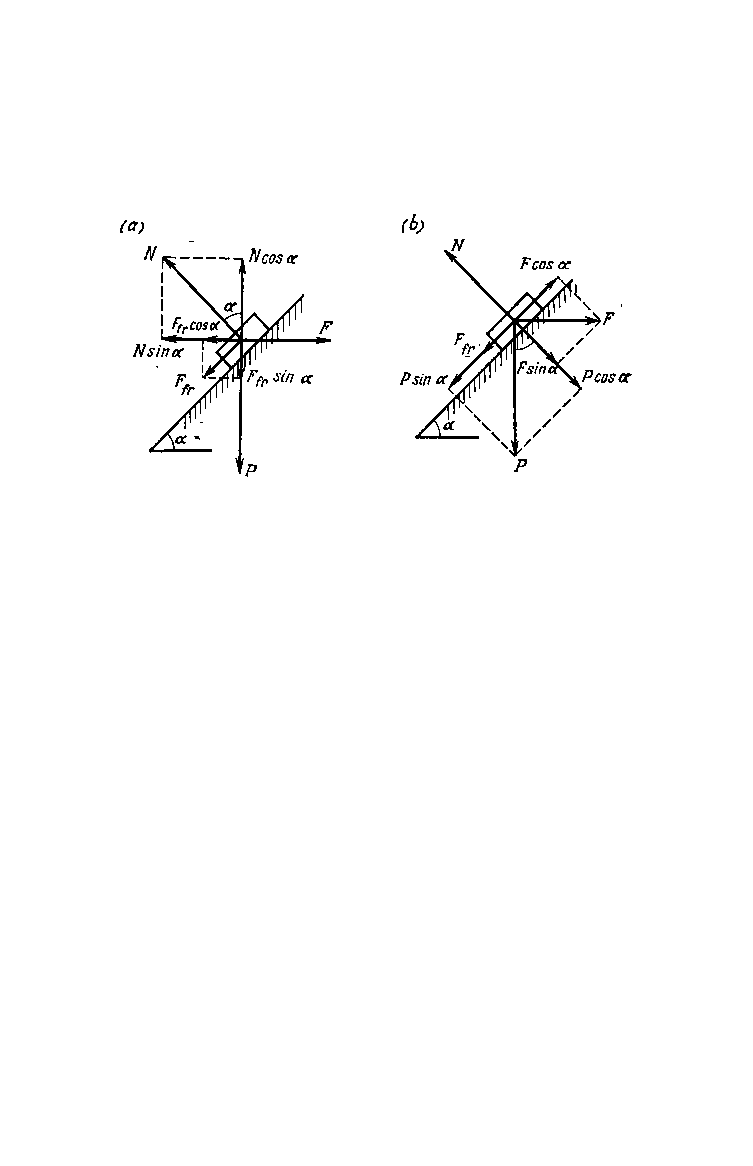
\includegraphics[width=\linewidth]{fig-027a.pdf}
\caption{Resolving the forces applied to a body in motion. }
\label{fig-27}
\end{figure}
After the forces have been resolved, the algebraic sums of the component forces for each direction of resolution are equated to zero (remember that we are still dealing with the motion of bodies without acceleration). For the case illustrated in \emph{Figure \ref{fig-27}(a)} we can write the system of equations
\begin{equation} 
\left.
\begin{split}
N \cos \alpha -F_{fr} \sin \alpha- P & = 0 \\
F - F_{fr} \cos \alpha - N \sin \alpha & = 0
\label{eq-21}
\end{split}
\right\}
\end{equation}
%\begin{equation} 
%\begin{split}
%(a+b)ˆ2 & = (a+b)(a+b)\\
% & = aˆ2+ab+ba+bˆ2\\
%& = aˆ2+2ab+bˆ2 
%\end{split}
%\end{equation}
The system of equations for the case in \emph{Figure \ref{fig-27}(b)} is
\begin{equation} 
\left.
\begin{split}
N  - P \cos \alpha -F \sin \alpha & = 0 \\
F_{fr} + P \sin \alpha - F \cos \alpha & = 0
\label{eq-22}
\end{split}
\right\}
\end{equation}

\textsc{Student:} But these systems of equations differ from each other.
\\
\textsc{Teacher:} They do but, nevertheless, lead to the same results, as can readily be shown. Suppose it is required to find the force $F$ that will ensure the motion of the body at uniform
velocity up along the inclined plane. Substituting equation (\ref{eq-005}) into equations (\ref{eq-21}) we obtain
\begin{equation*} 
\left.
\begin{split}
N  \left( \cos \alpha - k \sin \alpha \right)  - P & = 0 \\
F  - N \left( k \cos \alpha + \sin \alpha \right) & = 0
%\label{eq-22}
\end{split}
\right\}
\end{equation*}

From the first equation of this system we get
$$
N = \frac{P}{\cos \alpha -k \sin \alpha}
$$
which is substituted into the second equation to determine the required force. Thus
$$
F = P \left(\frac{k \cos \alpha + \sin \alpha }{\cos \alpha - k \sin \alpha}\right)
$$
Exactly the same answer is obtained from equations (\ref{eq-22}). You can check this for yourself.
\\
\textsc{Student:} What do we do if the body travels with acceleration?
\\
\textsc{Teacher:} In this case the choice of the directions of resolution depends on the direction in which the body is being accelerated (direction of the resultant force). Forces should be resolved in a direction along the acceleration and in one perpendicular to it. The algebraic sum of the force components in the direction perpendicular to the acceleration is equated to zero, while that of the force components in the direction along the acceleration is equal, according to Newton's second law of motion, to the product of the mass of the body by its acceleration.

Let us return to the body on the inclined plane in the last problem and assume that the body slides with a certain acceleration up the plane. According to my previous remarks, the forces should be resolved as in the case shown in \emph{Figure \ref{fig-27}(b)}. Then, in place of equations (\ref{eq-22}), we can write the following system
\begin{equation} 
\left.
\begin{split}
N  - P \cos \alpha -F \sin \alpha & = 0 \\
F \cos \alpha - F_{fr} - P \sin \alpha & = ma = P \left( \frac{a}{g} \right)
\label{eq-23}
\end{split}
\right\}
\end{equation}

Making use of equation (\ref{eq-005}), we find the acceleration of the body
\\
$$
a = \left( \frac{g}{p} \right) \left(F \cos \alpha - \left(P \cos \alpha + F \sin \alpha \right) k - P \sin \alpha \right) 
$$
\textsc{Student:} In problems of this kind dealing with acceleration, can the forces be resolved in directions other than along the acceleration and perpendicular to it? As far as I understand from your explanation, this should not be done.
\\
\textsc{Teacher:} Your question shows that I should clear up some points. Of course, even in problems on acceleration you have a right to resolve the forces in any two mutually perpendicular directions. In this case, however, you will have to resolve not only the forces, but the acceleration vector as well. This method of solution will lead to additional difficulties. To avoid unnecessary complications, it is best to proceed exactly as is advised. This is the simplest course. The direction of the body's acceleration is always known (at least its sign), so you can proceed on the basis of this direction. The inability of examinees to choose the directions of force resolution rationally is one of the reasons for their helplessness in solving more or less complex problems in dynamics.
\\
\textsc{Student:} We have only been speaking about resolution in two directions. In the general case, however, it would probably be more reasonable to speak of resolution in three mutually perpendicular directions. Space is actually three-dimensional.
\\
\textsc{Teacher:} You are absolutely right. The two directions in our discussions are explained by the fact that we are dealing with plane (two-dimensional) problems. In the general case, forces should be resolved in three directions. All the remarks made above still hold true, however. I should mention that, as a rule, two-dimensional problems are given in examinations. Though, of course, the examinee may be asked to make a not-too-complicated generalization for the three-dimensional case.
\newpage
\section{PROBLEMS}
\label{problems-02}
%\begin{fullwidth}

\begin{enumerate}[resume*=problems]
\item A body with a mass of \SI{5}{kg} is pulled along a horizontal plane by a force of \SI{3}{\newton}\sidenote{Originally unit of \emph{kgf} is used, here after we will use the unit of Newtons denoted by \si{\newton}.} applied to the body at an angle of \ang{30} to the horizontal. The coefficient of sliding friction is 0.2. Find the velocity of the body \SI{10}{\second} after the pulling force begins to act, and the work done by the friction force during this time.

\item A man pulls two sleds tied together by applying a force of $F=$ \SI{12}{\newton} to the pulling rope at an angle of \ang{45} to the horizontal (\emph{Figure \ref{fig-28}}). The masses of the sleds are equal to $m_{1}=m_{2}=$ \SI{15}{\kilogram}. The coefficient of friction between the runners and the snow is 0.02. Find the acceleration of the sleds. the tension of the rope tying the sleds together, and the force with which the man should pull the rope to impart uniform velocity to the sleds.

\begin{marginfigure}[-4cm]
\centering
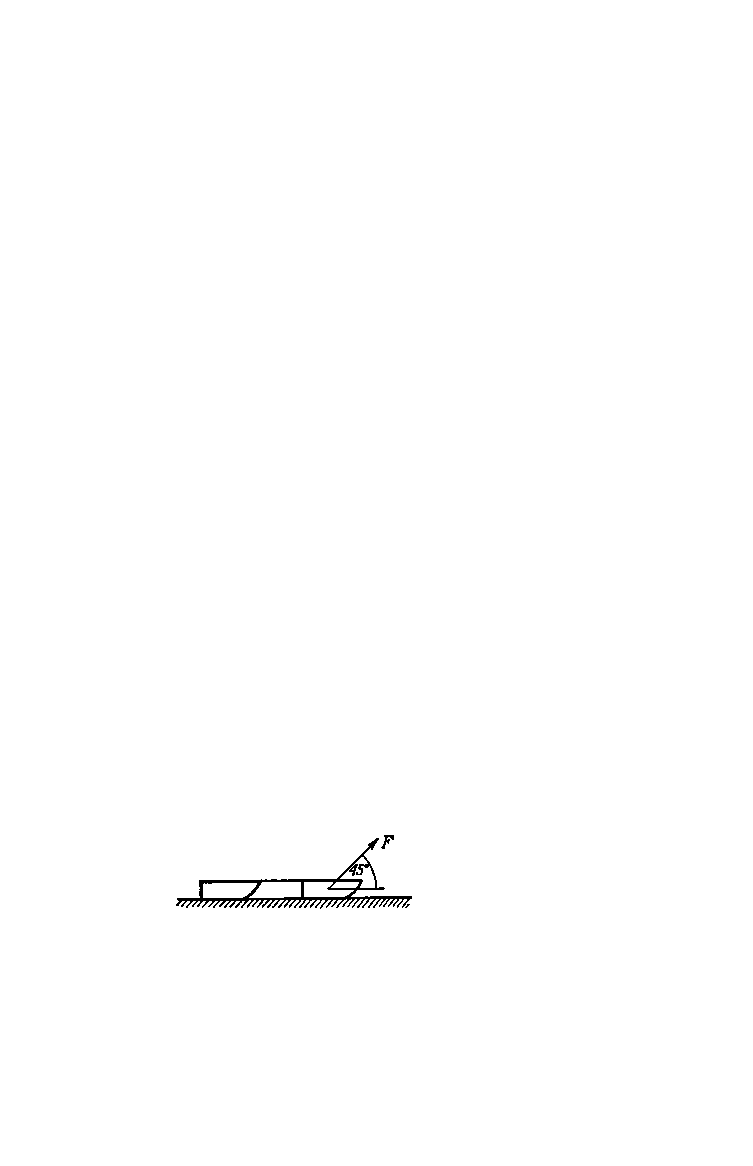
\includegraphics[width=0.9\linewidth]{fig-028a.pdf}
\caption{Sled being pulled by a rope with an angle \ang{45}. See problem 9.}
\label{fig-28}
\end{marginfigure}
\item Three equal weights of a mass of \SI{2}{\kilogram} each are hanging on a string passing over a fixed pulley as shown in \emph{Figure \ref{fig-29}}. Find the acceleration of the system and the tension of the string connecting weights 1 and 2.
\begin{marginfigure}
\centering
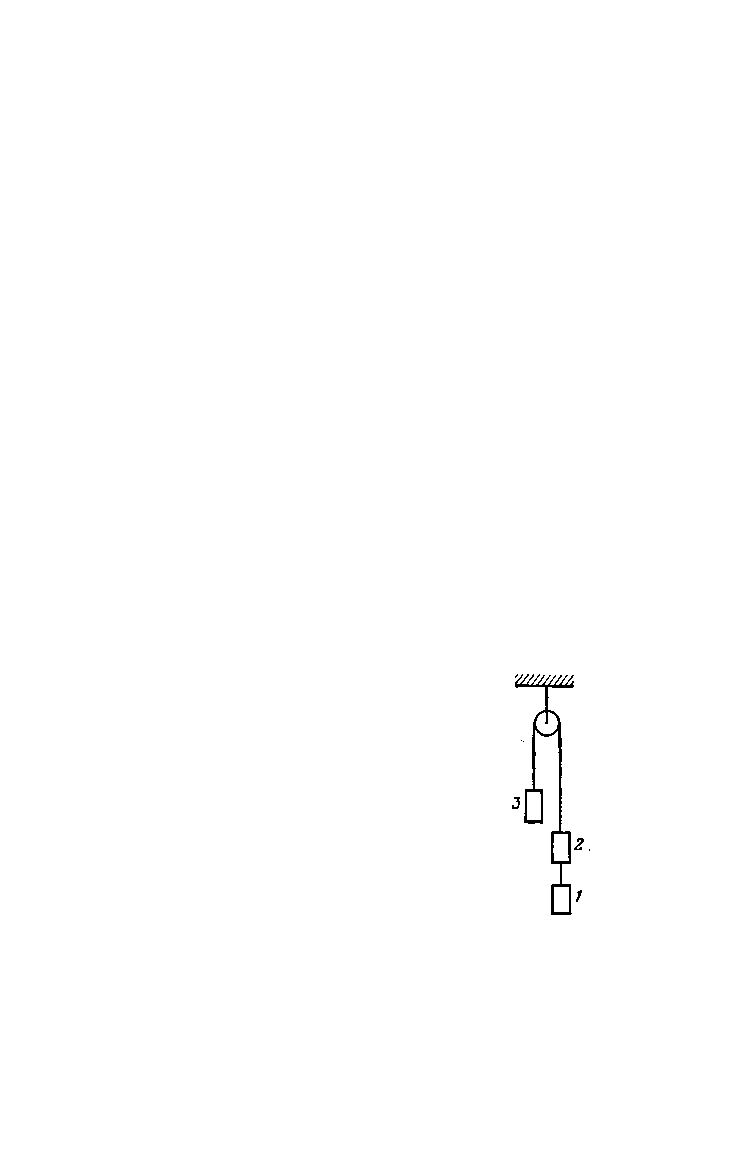
\includegraphics[width=0.4\linewidth]{fig-029a.pdf}
\caption{A system of three interacting masses.  See problem 10.}
\label{fig-29}
\end{marginfigure}

\item Calculate the acceleration of the weights and the tension in the strings for the case illustrated in \emph{Figure \ref{fig-30}}. Given: $\alpha = \ang{30}$, $P_{1}=\SI{4}{\newton}$, $P_{2}=\SI{2}{newton}$, and $P_{3}=\SI{8}{\newton}$. Neglect the friction between the weights and the inclined plane.
\begin{marginfigure}
\centering
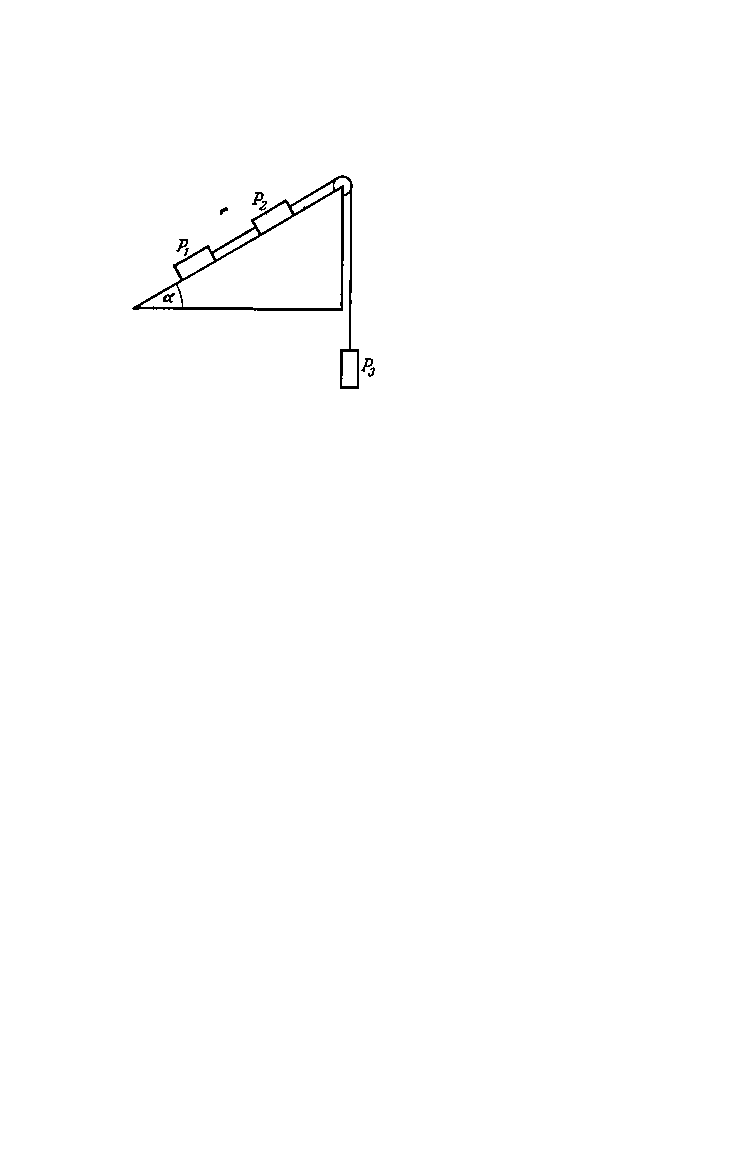
\includegraphics[width=0.8\linewidth]{fig-030a.pdf}
\caption{A system of three masses on an incline. See problem 11.}
\label{fig-30}
\end{marginfigure}

\item Consider the system of weights shown in \emph{Figure \ref{fig-31}}. Here $P_{1}=\SI{1}{\newton}$$P_{2}=\SI{2}{\newton}$, $P_{5}=\SI{8}{\newton}$ and $P_{4}=\SI{0.5}{\newton}$, and $\alpha=\ang{30}$. The coefficient of friction between the weights and the planes equals 0.2. Find the acceleration of the set of weights, the tension of the strings and the force with which
weight $P_{4}$ presses downward on weight $P_{3}$.
\begin{marginfigure}
\centering
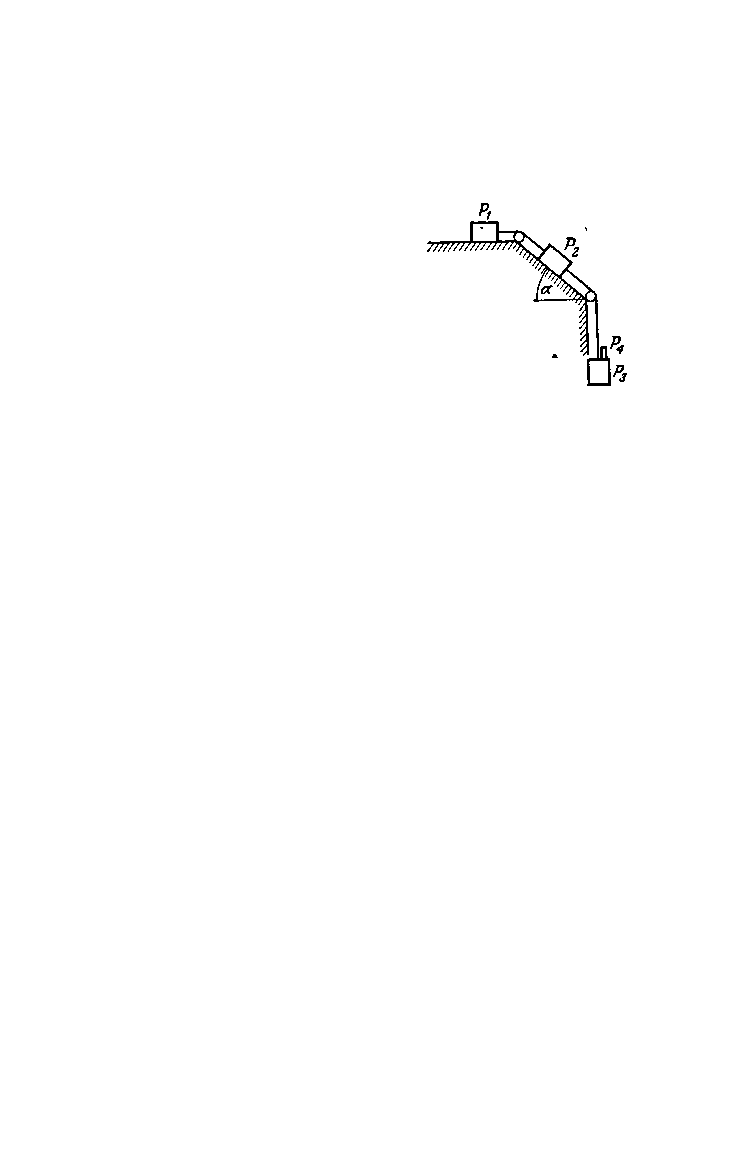
\includegraphics[width=0.8\linewidth]{fig-031a.pdf}
\caption{A system of three masses on an incline. See problem 12}
\label{fig-31}
\end{marginfigure}
\end{enumerate}
%\end{fullwidth}
\chapter{Are Problems In Dynamics Much More Difficult To Solve If Friction Is Taken Into Account?}
\label{ch-07}
\paragraph{}
\textsc{Teacher:} Problems may become much more difficult when the friction forces are taken into account.
\\
\textsc{Student:} But we have already discussed the force of friction (Chapter \ref{ch-03}). If a body is in motion, the friction force is determined from the bearing reaction ($F_{fr}=kN$); if the body is at rest, the friction force is equal to the force that tends to take it out of this state of rest. All this can readily be understood and remembered.
\\
\textsc{Teacher:} That is so. However, you overlook one important fact. You assume that you already know the answers to the following questions: 
\begin{enumerate}[label=(\arabic*),leftmargin=1cm]
\item Is the body moving or is it at rest? 
\item In which direction is the body moving (if at all)? 
\end{enumerate}

If these items are known beforehand, then the problem is comparatively simple. Otherwise, it may be very complicated from the outset and may even require special investigation.
\\
\textsc{Student:} Yes, now I recall that we spoke of this matter in Chapter \ref{ch-02} in connection with our discussion concerning the choice of the direction of the friction force.
\\
\textsc{Teacher:} Now I want to discuss this question in more detail. It is my firm opinion that the difficulties involved in, solving problems which take the friction force into account are obviously underestimated both by students and by certain authors who think up problems for physics textbooks.

\emph{Let us consider the example illustrated in \emph{Figure \ref{fig-10}}. The angle of inclination $\alpha$ of the plane, weight $P$ of the body, force $F$ and the coefficient of friction $k$ are given. For simplicity we shall assume that $k_{0}=k$ (where $k_{0}$ is the coefficient determining the maximum possible force of static friction). It is required to determine the kind of motion of the body and to find
the acceleration.}

Let us assume that the body slides upward along the inclined surface. We can resolve the forces as shown in \emph{Figure \ref{fig-27}(b)} and make use of the result obtained for the acceleration in  Chapter \ref{ch-06}.Thus
\begin{equation}
a = \frac{g}{P} \left[F \cos \alpha- P \sin \alpha -(P \cos \alpha + F \sin \alpha) \, k \right]
\label{eq-24}
\end{equation}


It follows from equation (\ref{eq-24}) that for the body to slide upward along the inclined plane, the following condition must be complied with:
$$
F \cos \alpha - P \sin \alpha -\left( P \cos \alpha + F \sin \alpha \right) k \geqslant 0
$$
This condition can be written in the form
$$
F \geqslant P \left ( \frac{k \cos \alpha + \sin \alpha}{\cos \alpha -k \sin \alpha} \right)
$$
or
\begin{equation}
F \geqslant P \left ( \frac{k + \tan \alpha}{ 1 -k \tan \alpha} \right)
\label{eq-25}
\end{equation}

We shall also assume that the angle of inclination of the plane is not too large, so that $(1-k \tan \alpha)$ or 
\begin{equation}
\tan \alpha < \frac{1}{k}
\label{eq-26}
\end{equation}
We shall next assume that the body slides downward along the inclined plane. We again resolve all the forces as in \emph{Figure \ref{fig-27}(b)} but reverse the friction force. As a result we obtain the fall owing expression for the acceleration of the body 
\begin{equation}
a= \frac{g}{P} \left[P \sin \alpha -F \cos \alpha - \left( P \cos \alpha + F \sin \alpha \right) \, k \right]
\label{eq-27}
\end{equation}
From equation (\ref{eq-27}) it follows that for the body to slide downward along the inclined plane, the following condition must be met:
$$
P \sin \alpha -F \cos \alpha - \left( P \cos \alpha + F \sin \alpha \right) k \geqslant 0
$$

This condition we write in the form
\begin{equation*}
F \leqslant P \left ( \frac{ \sin \alpha - k \cos \alpha}{\cos \alpha + k \sin \alpha} \right)
%\label{eq-25}
\end{equation*}
or

\begin{equation}
F \leqslant P \left ( \frac{ \tan \alpha -k }{ 1 + k \tan \alpha} \right)
\label{eq-28}
\end{equation}

In this case, we shall assume that the angle of inclination of the plane is not too small, so that $(\tan \alpha- k)>0$, or
\begin{equation}
\tan \alpha > k
\label{eq-29}
\end{equation}
Combining conditions (\ref{eq-25}), (\ref{eq-26}), (\ref{eq-28}) and (\ref{eq-29}), we can come to
the following conclusions:

\begin{enumerate}[label=\textbf{(\arabic*)},leftmargin=1cm]
\item Assume that the condition
\begin{equation*}
k < \tan \alpha < \frac{1}{k}
\end{equation*}

holds good for an inclined plane. Then:
\begin{enumerate}[label=\textbf{(\alph*)},leftmargin=1cm]
\item if $F>P \left(\dfrac{k+\tan \alpha}{ 1-k \tan \alpha}\right)$, the body slides upward with an acceleration that can be determined by equation (\ref{eq-24});
\item if $F=P \left(\dfrac{k+\tan \alpha}{ 1-k \tan \alpha}\right)$, the body slides upward at uniform velocity or is at rest;
\item if $F<P \left(\dfrac{\tan \alpha - k}{ 1+k \tan \alpha}\right)$, the body slides downward with an acceleration that can be determined by equation (\ref{eq-27});
\item if $F=P \left(\dfrac{\tan \alpha-k}{1+k \tan \alpha}\right)$, the body slides downward with uniform velocity or is at rest;
\item if $P\left( \dfrac{\tan \alpha-k}{1+k \tan \alpha}\right) < F < P \left( \dfrac{k+\tan \alpha}{1-k \tan \alpha} \right)$, the body is at rest.
\end{enumerate}

Note that upon increase in force $F$ from $P \left(\dfrac{\tan \alpha-k}{1 +k \tan \alpha}\right)$ to $P \left( \dfrac{k+\tan \alpha} {1-k \tan \alpha} \right)$, the force of static friction is gradually reduced from $k (P \cos \alpha +F \sin \alpha)$ to zero; then, after its direction is reversed, it increases to the value $k (P \cos \alpha +F \sin \alpha)$. While this goes on the body remains at rest.
	 
\item Now assume that the inclined plane satisfies the condition
\begin{equation*}
0 < \tan \alpha \leqslant k
\end{equation*}

then:

\begin{enumerate}[label=\textbf{(\alph*)},leftmargin=1cm]
\item if $F>P \left(\dfrac{k+\tan \alpha}{ 1-k \tan \alpha}\right)$, the body slides upward with an acceleration that can be determined by equation (24);
\item if  $F=P \left(\dfrac{k+\tan \alpha}{ 1-k \tan \alpha}\right)$, the body slides upward at uniform velocity or is at rest;
\item if  $F<P \left(\dfrac{k+\tan \alpha}{ 1-k \tan \alpha}\right)$, the body is at rest; no downward motion of the body along the inclined plane is possible (even if force $F$ vanishes).
\end{enumerate}

\item Finally, let us assume that the inclined plane meets the condition 
\begin{equation*}
\tan \alpha \geqslant \frac{1}{k}
\end{equation*}
then:
\begin{enumerate}[label=\textbf{(\alph*)},leftmargin=1cm]
\item if $F< P \left(\dfrac{\tan \alpha - k}{ 1 + k \tan \alpha}\right)$, the body slides downward with an acceleration that can be determined by equation (\ref{eq-27});
\item if $F = P \left(\dfrac{\tan \alpha - k}{ 1 + k \tan \alpha}\right)$, the body slides down ward with uniform velocity or is at rest;
\item if $F > P \left(\dfrac{\tan \alpha - k}{ 1 + k \tan \alpha}\right)$, the body is at rest; no upward motion of the body along the inclined plane is possible. On the face of it, this seems incomprehensible because force $F$ can be increased indefinitely! The inclination of the plane is so large, however, that, with an increase in force F, the pressure of the body against the plane will increase at an even faster rate.
\end{enumerate}
\end{enumerate}

\textsc{Student:} Nothing of the kind has ever been demonstrated to us in school. 
\\
\textsc{Teacher:} That is exactly why I wanted to draw your attention to this matter. Of course, in your entrance examinations you will evidently have to deal with much simpler cases: there will be no friction, or there will be friction but the nature of the motion will be known beforehand (for instance, whether the body is in motion or at rest). However, even if one does not have to swim over deep spots, it is good to know where they are.
\\
\textsc{Student:} What will happen if we assume that $k=0$?
\\
\textsc{Teacher:} In the absence of friction, everything becomes much simpler at once. For any angle of inclination of the plane, the results will be: 
\begin{enumerate}[label=$\blacktriangleright$,leftmargin=1cm]
\item at $F > P \tan \alpha$, the body slides upward with the acceleration 

\begin{equation}
a = \frac{g}{P} \left( F \cos \alpha -P \sin \alpha \right)
\label{eq-30}
\end{equation}

\item at $F = P \tan \alpha$, the body slides with uniform velocity (upward or downward) or is at rest;

\item at $F < P \tan \alpha$, the body slides downward with an acceleration

\begin{equation}
a = \frac{g}{P} \left( P \sin \alpha - F \cos \alpha \right)
\label{eq-31}
\end{equation}

\end{enumerate}
Note that the results of equations (\ref{eq-30}) and (\ref{eq-31}) coincide with an accuracy to the sign. Therefore, in solving problems, you can safely assume any direction of motion, find $a$ and take
notice of -the sign of the acceleration. If $a>0$, the body travels in the direction you have assumed; if $a<0$, the body will travel in the opposite direction (the acceleration will be equal to $|a|$.

Let us consider one more problem. \emph{Two bodies $P_{1}$ and $P_{2}$ are connected by a string running over a pulley. Body $P_{1}$ is on an inclined plane with the angle of inclination $\alpha$ and coefficient of friction $k$; body $P_{2}$ hangs on the string (\emph{Figure \ref{fig-32}}). Find the acceleration of the system.}

\begin{figure}
\centering
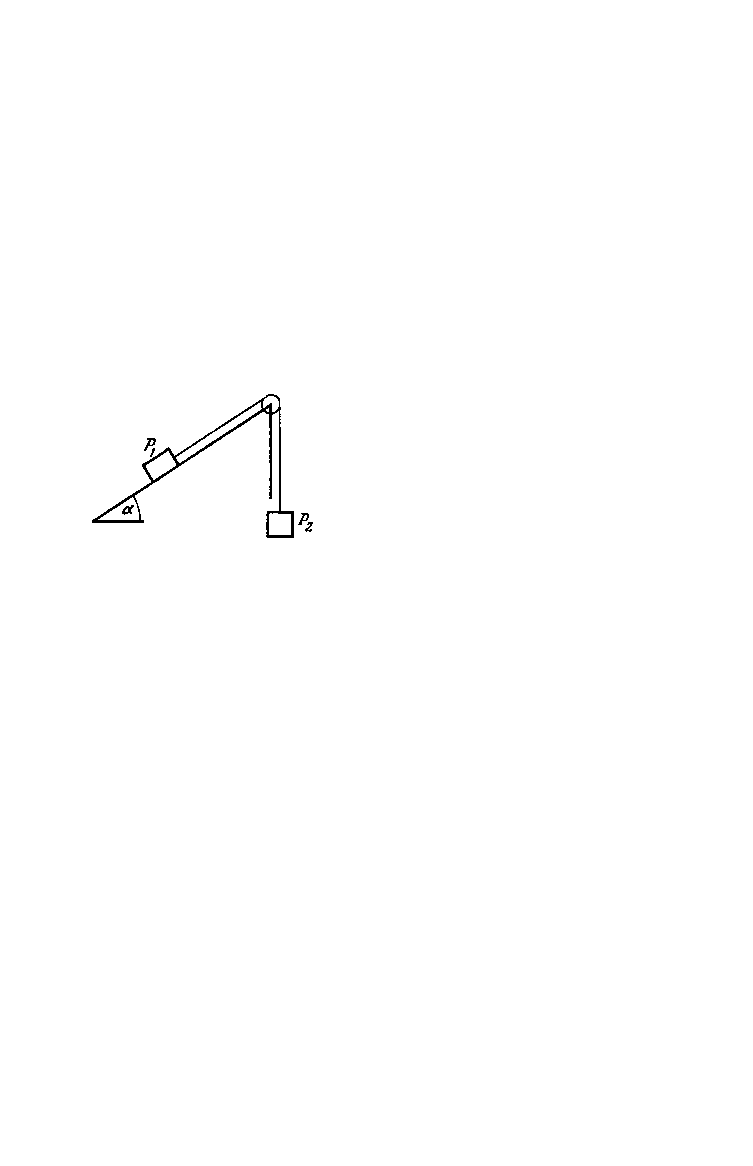
\includegraphics[width=0.4\linewidth]{fig-032a.pdf}
\caption{Two bodies connected via string on an inclined plane. The problem is to find the acceleration of the system.}
\label{fig-32}
\end{figure}

Assume that the system is moving from left to right. Considering the motion of the system as a whole, we can write the following equation for the acceleration:

\begin{equation}
a = g \left( \frac{P_{2} - P_{1} \sin \alpha - P_{1} k \cos \alpha}{P_{1}+P_{2}}\right)
\label{eq-32}
\end{equation}

Assuming now that the system moves from right to left, we obtain

\begin{equation}
a = g \left( \frac{P_{1} \sin \alpha - P_{2} - P_{1} k \cos \alpha}{P_{1}+P_{2}}\right)
\label{eq-33}
\end{equation}

We will carry out an investigation for the given $\alpha$, and $k$ values, varying the ratio $p=\dfrac{P_{2} }{P_{1}}$. From equation (\ref{eq-32}) it follows that for motion from left to right, the condition 

\begin{equation*}
p \leqslant \frac{1}{\sin \alpha + k \cos \alpha}
\end{equation*}

should be met. Equation (\ref{eq-33}) implies that for motion from right to left the necessary condition is

\begin{equation*}
p \geqslant \frac{1}{\sin \alpha - k \cos \alpha}
\end{equation*}

Here an additional condition is required: the angle of inclination should not be too small, i.e. $\tan \alpha >k$ . If $\tan \alpha \leqslant k$, then the system will not move from right to left, however large the ratio $p$ may be. If $\tan \alpha >k$, the body is at rest provided the following inequality holds true:

\begin{equation*}
 \frac{1}{\sin \alpha + k \cos \alpha} < p < \frac{1}{\sin \alpha - k \cos \alpha}
\end{equation*}

If, instead, $\tan \alpha \leqslant k$, then the body is at rest at

\begin{equation*}
p > \frac{1}{\sin \alpha + k \cos \alpha}
\end{equation*}

\textsc{Student:} And what will happen if we change the angle $\alpha$ or the coefficient $k$?
\\
\textsc{Teacher:} I leave investigation from this point of view to you as a home assignment (see Problems Nos. 13 and 14).
\\
\section{PROBLEMS}
\label{problems-03}

\begin{enumerate}[resume*=problems]
\item Investigate the problem illustrated in \emph{Figure \ref{fig-32}} assuming that the
angle $\alpha$ of inclination of the plane and the ratio $p=\dfrac{P_{2} }{P_{1}}$ are given, and
assigning various values to the coefficient $k$.
\item Investigate the problem illustrated in \emph{Figure \ref{fig-32}}, assuming that the
coefficient of friction $k$ and the ratio $p=\dfrac{P_{2} }{P_{1}}$ are given and assigning
various values to the angle $\alpha$ of inclination of the plane. For the sake of
simplicity, use only two values of the ratio: $p= 1$ (the bodies are of equal
weight) and $p= \dfrac{1}{2}$ (the body on the inclined plane is twice as heavy as
the one suspended on the string).
\end{enumerate}
\cleardoublepage
\thispagestyle{empty}
\vspace*{2cm}

\begin{figure*}
\centering
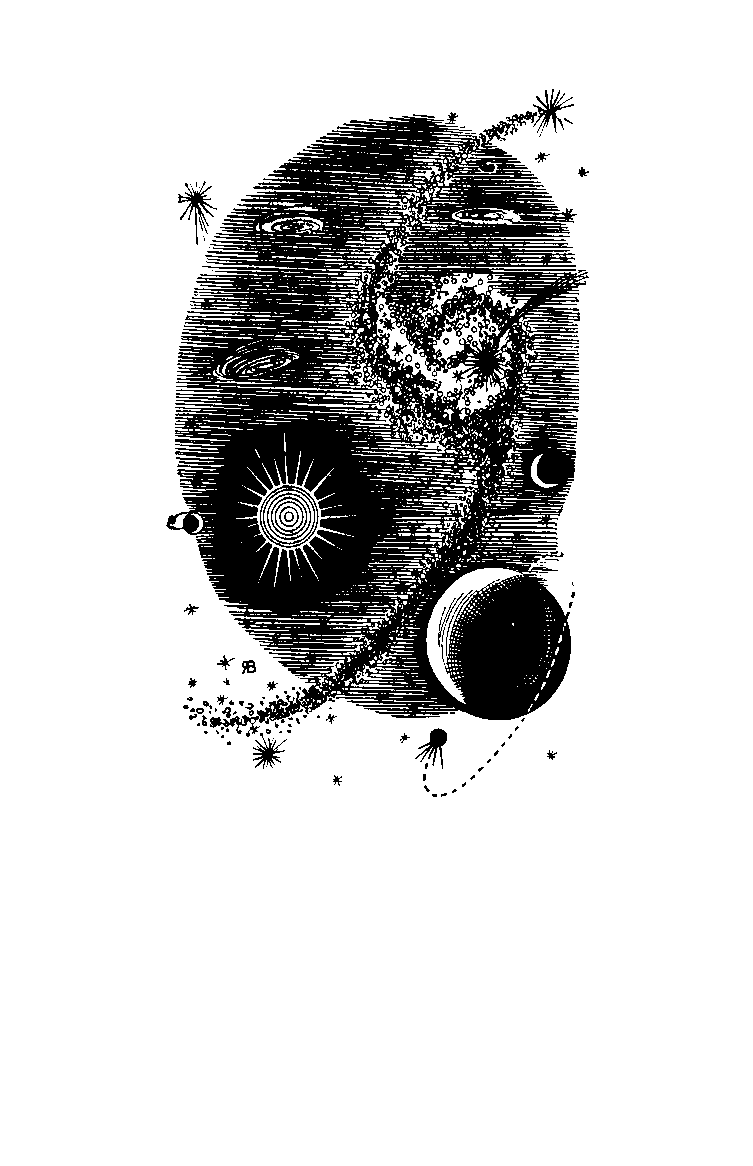
\includegraphics[width=0.65\linewidth]{sec-c.pdf}
%\caption{Velocity \emph{vs} time graph for the function shown in Figure \ref{fig-05}.}
%\label{fig-06}
\end{figure*}
%\addtocounter{figure}{1}
% For incrementing the figure numbers for figures without caption or numbering
\begin{fullwidth}
\begin{Large}
Motion in a circle is the simplest form of curvilinear motion. The more important it is to comprehend the specific features of such motion. You can see that the whole universe is made up of curvilinear motion. Let us consider uniform and non-uniform motion of a material point in a circle, and the motion of orbiting satellites. This will lead us to a discussion of the physical causes of the weightlessness of bodies.
\end{Large}
\end{fullwidth}

\chapter{How Do You Deal With Motion In A Circle?}
\label{ch-08}

\textsc{Teacher:} I have found from experience that questions and problems concerning motion of a body in a circle turn out to be extremely difficult for many examinees.Their answers to such questions contain a great many typical errors. To demonstrate this let us invite another student
to take part in our discussion. This student doesn't know what we have discussed previously. We shall conditionally call him ``\textsf{\textbf{Student B}} '' (the first student will hereafter be called ``\textsf{\textbf{Student A}}'').

Will Student B please indicate the forces acting on a satellite, or sputnik, in orbit around the earth? We will agree to neglect the resistance of the atmosphere and the attraction of the moon, sun and other celestial bodies.
\\
\textsc{Student B:} The satellite is subject to two forces: the attraction of the earth and the centrifugal force.
\\
\textsc{Teacher:} I have no objections to the attraction of the earth, but I .don't understand where you got the centrifugal force from. Please explain.
\\
\textsc{Student B:} If there were no such force, the satellite could not stay in orbit.
\\
\textsc{Teacher:} And what would happen to it?
\\
\textsc{Student B:} Why, it would fall to the earth.
\\
\textsc{Teacher:} (turning to Student A): Remember what I told you before! This is a perfect example of an attempt to prove that a certain force exists, not on the basis of the interaction of bodies, but by a backdoor manoeuvre - from the nature of the motion of bodies. As you see, the satellite must stay in orbit, so it is necessary to introduce a retaining force. Incidentally, if this centrifugal force really did exist, then the satellite could not remain in orbit because the forces acting on the satellite would cancel out and it would fly at uniform velocity and in a straight line.
\\
\textsc{Student A:} The centrifugal force is never applied to a rotating body. It is applied to the tie (string or another bonding member). It is the centripetal force that is applied to the rotating body.
\\
\textsc{Student B:} Do you mean that only the weight is applied to the satellite?
\\
\textsc{Teacher:} Yes, only its weight.
\\
\textsc{Student B:} And, nevertheless, it doesn't fall to the earth?
\\
\textsc{Teacher:} The motion of a body subject to the force of gravity is called falling. Hence, the satellite is falling. However, its ``falling'' is in the form of motion in a circle around the earth and therefore can continue indefinitely. We have already established that the direction of motion of a body and the forces acting on it do not necessarily coincide (see Chapter \ref{ch-04}).
\\
\textsc{Student B:} In speaking of the attraction of the earth and the centrifugal force, I based my statement on the formula 
\begin{equation}
\frac{GmM}{r^{2}} = \frac{mv^{2}}{r}
\label{eq-34}
\end{equation}

where the left-hand side is the force of attraction ($m$=mass of the satellite, $M$ =mass of the earth, $r$=radius of the orbit and $G$=gravitational constant), and the right-hand side is the centrifugal force ($v$=velocity of the satellite). Do you mean to say that this formula is incorrect?
\textsc{Teacher:} No, the formula is quite correct. What is incorrect is your interpretation of the formula. You regard equation (\ref{eq-34}) as one of equilibrium between two forces. Actually, it is an expression of Newton's second law of motion
\begin{equation}
F = ma
\tag{34(a)}
\label{eq-34a}
\end{equation}
where $F=\dfrac{GmM}{r^{2}}$ and $a=\left( \dfrac{v^{2}}{r} \right)$ is the centripetal acceleration.
\\
\textsc{Student B:} I agree that your interpretation enables us to get along without any centrifugal force. But, if there is no centrifugal force, there must at least be a centripetal force. You have not, however, mentioned such a force.
\\
\textsc{Teacher:} In our case, the centripetal force is the force of attraction between the satellite and the earth. I want to underline the fact that this does not refer to two different forces. By no means. This is one and the same force.
\\
\textsc{Student B:} Then why introduce the concept of a centripetal force at all?
\\
\textsc{Teacher:} I fully agree with you on this point. The term ``centripetal force'', in my opinion, leads to nothing but confusion. What is understood to be the centripetal force is not at all an independent force applied to a body along with other forces. It is, instead, the resultant of all the forces
applied to a body travelling in a circle at uniform velocity.

The quantity $\left(\dfrac{mv^{2}}{r} \right)$  is not a force. It represents the product of the mass $m$ of the body by the centripetal acceleration $\left(\dfrac{v^{2}}{r}\right)$. This acceleration is directed toward the centre and, consequently, the resultant of all forces, applied to a body travelling in a circle at uniform velocity, is directed toward the centre. Thus, there is a centripetal acceleration and there are forces which, added together, impart a centripetal acceleration to the body.\\
\textsc{Student B:} I must admit that this approach to the motion of a body in a circle is to my liking. Indeed, this motion is not a static case, for which an equilibrium of forces is characteristic, but a dynamic case.
\\
\textsc{Student A:} If we reject the concept of a centripetal force, then we should probably drop the term ``centrifugal force'' as well, even in reference to ties.
\\
\textsc{Teacher:} The introduction of the term ``centrifugal force'' is even less justified. The centripetal force actually exists, if only as a resultant force. The centrifugal force does not even exist in many cases.
\\
\textsc{Student A:} I don't understand your last remark. The centrifugal force is introduced as a reaction to the centripetal force. If it does not always exist, as you say, then Newton's third law of motion is not always valid. Is that so?
\\
\textsc{Teacher:} Newton's third law is valid only for real forces determined by the interaction of bodies, and not for the resultants of these forces. I can demonstrate this by the example of the conical pendulum that you are already familiar with (\emph{Figure \ref{fig-33}}). 

\begin{figure}
\centering
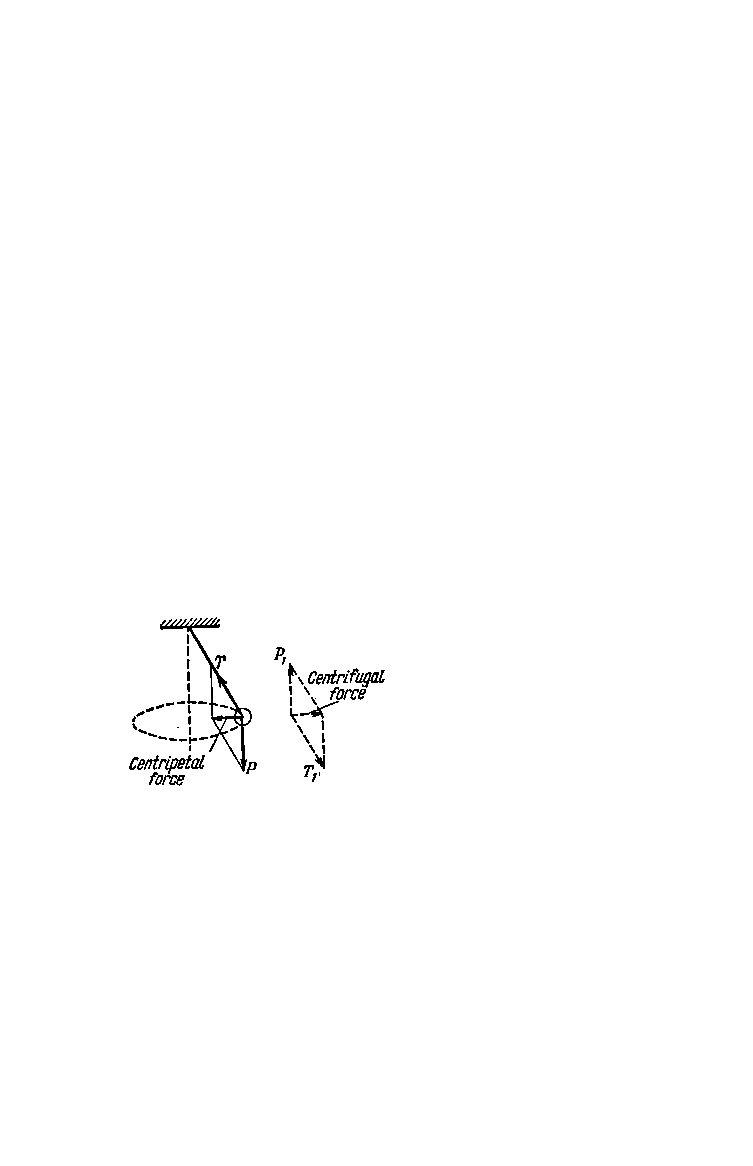
\includegraphics[width=0.6\linewidth]{fig-033a.pdf}
\caption{A conical pendulum. The body attached to the string performs circular motion in the horizontal plane. During this motion the solid that it traces has cone shape.}
\label{fig-33}
\end{figure}

The ball is subject to two forces: the weight $P$ and the tension $T$ of the string. These forces, taken together, provide the centripetal acceleration of the ball, and their sum is called the centripetal force. Force $P$ is due to the interaction of the ball with the earth. The reaction of this force is force $P_{1}$ which is applied to the earth. Force $T$ results from interaction between the ball and the string. The reaction of this force is force $T_{1}$ which is applied to the string. If forces $P_{1}$ and $T_{1}$ are formally added together we obtain a force which is conventionally understood to be the centrifugal force
(see the dashed line in \emph{Figure \ref{fig-33}}). But to what is this force applied? Are we justified in calling it a force when one of its components is applied to the earth and the other to an entirely different body-the string? Evidently, in the given case, the concept of a centrifugal force has no physical meaning.
\\
\textsc{Student A:} In what cases does the centrifugal force exist?
\\
\textsc{Teacher:} In the case of a satellite in orbit, for instance, when only two bodies interact -the earth and the satellite. The centripetal force is the force with which the earth attracts the satellite. The centrifugal force is the force with which the satellite attracts the earth.
\\
\textsc{Student B:} You said that Newton's third law was not valid for the resultant of real forces. I think that in this case it will be invalid also for the components of a real force. Is that true?
\\
\textsc{Teacher:} Yes, quite true. In this connection I shall cite an example which has nothing in common with rotary motion. A ball lies on a floor and touches a wall which makes an obtuse
angle with the floor (\emph{Figure \ref{fig-34}}). 

\begin{figure}
\centering
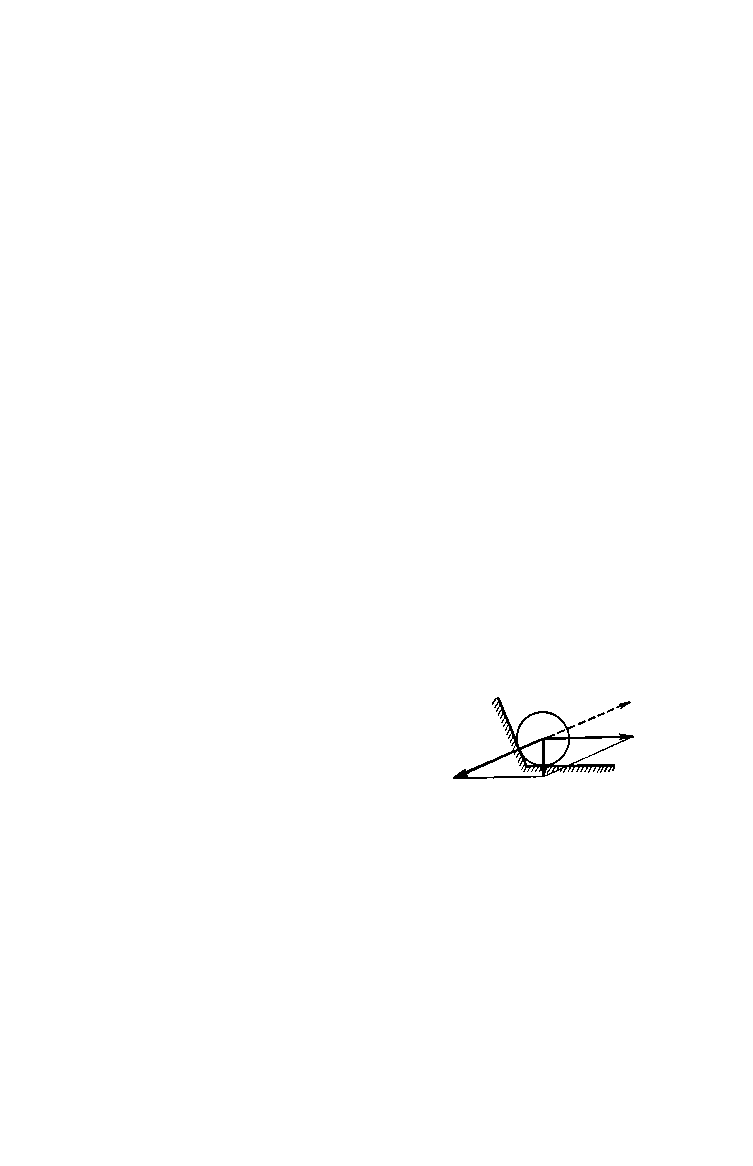
\includegraphics[width=0.6\linewidth]{fig-034a.pdf}
\caption{A on the floor touching a wall at an obtuse angle with the floor.}
\label{fig-34}
\end{figure}

Let us resolve the weight of the ball into two components: perpendicular to the wall and parallel to the floor. We shall deal with these two components instead of the weight of the ball. If Newton's third law were applicable to separate components, we could expect a reaction of the wall counter balancing the component of the weight perpendicular to it. Then, the component of the weight parallel to the floor would remain unbalanced and the ball would have to have a horizontal acceleration. Obviously, this is physically absurd.
\\
\textsc{Student A:} So far you have discussed uniform motion in a circle. How do you deal with a body moving non-uniformly in a circle? For instance, a body slides down from the top of a vertically held hoop. While it slides along the hoop it is moving in a circle. This cannot, however, be uniform motion because the velocity of the body increases. What do you, do in such cases?
\\
\textsc{Teacher:} If a body moves in a circle at uniform velocity, the resultant of all forces applied to the body must be directed to the centre; it imparts centripetal acceleration to the body. In the more general case of nonuniform motion in a circle, the resultant force is not directed strictly toward the centre. In this case, it has a component along a radius toward the centre and another component tangent to the trajectory of the body (i.e. to the circle). The first component is responsible for the centripetal acceleration of the body, and the second component, for the so-called tangential acceleration, associated with the change in velocity. It should be pointed out that since the velocity of the body changes, the centripetal acceleration $\left(\dfrac{v^{2}}{r}\right)$ must also change.
\\
\textsc{Student A:} Does that mean that for each instant of time the centripetal acceleration will be determined by the formula $a = \left(\dfrac{v^{2}}{r}\right)$, where $v$ is the instantaneous velocity?
\\
\textsc{Teacher:} Exactly. While the centripetal acceleration is constant in uniform motion in a circle, it varies in the process of motion in nonuniform motion in a circle.
\\
\textsc{Student A:} What does one do to find out just how the velocity $v$ varies in nonuniform rotation?
\\
\textsc{Teacher:} Usually, the law of conservation of energy is resorted to for this purpose. Let us consider a specific example.
\emph{Assume that a body slides without friction from the top of a vertically held hoop of radius $R$. With what force will the body press on the hoop as it passes a point located at a height $h$ \si{\centi\metre} below the top of the hoop? The initial velocity of the body at the top of the hoop equals zero.} 

First of all, it is necessary to find what forces act on the body.
\\
\begin{figure}
\centering
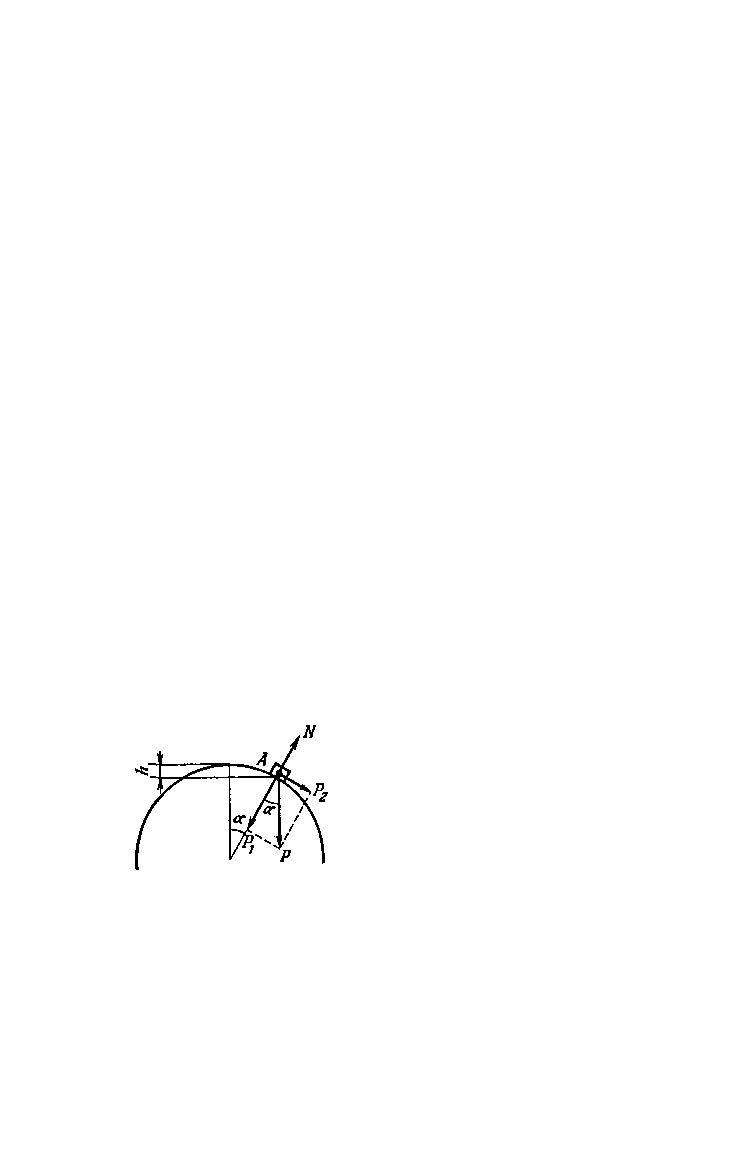
\includegraphics[width=0.6\linewidth]{fig-035a.pdf}
\caption{A on the floor touching a wall at an obtuse angle with the floor.}
\label{fig-35}
\end{figure}
\textsc{Student A:} Two forces act on the body: the weight $P$ and
the bearing reaction $N$. They are shown in Fig. 35.
\\
\textsc{Teacher:} Correct. What are you going to do next?
\\
\textsc{Student A:} I'm going to do as you said. I shall find the resultant of these two forces and resolve it into two components: one along the radius and the other tangent to the circle.
\\
\textsc{Teacher:} Quite right. Though it would evidently be simpler to start by resolving the two forces applied to the body in the two directions instead of finding the resultant, the more so because it will be necessary to resolve only one force-the weight.
\\
\textsc{Student A:} My resolution of the forces is shown in \emph{Figure \ref{fig-35}}.
\\
\textsc{Teacher:} Force $P_{2}$ is responsible for the tangential acceleration of the body, it does not interest us at present. The resultant of forces $P_{1}$ and $N$ causes the centripetal acceleration of the body, i.e.
\begin{equation}
P_{1} - N = \frac{mv^{2}}{R}
\label{eq-35}
\end{equation}

The velocity of the body at the point we are interested in (point $A$ in \emph{Figure \ref{fig-35}}) can be found from the law of conservation of energy
\begin{equation}
Ph = \frac{mv^{2}}{2}
\label{eq-36}
\end{equation}

Combining equations (\ref{eq-35}) and (\ref{eq-36}) and taking into consideration that
\begin{equation*}
P_{1}=P \cos \alpha = P \left(\frac{R-h}{R}\right),
\end{equation*}
 we obtain
\begin{equation*}
\frac{P}{R} \left( R-h \right) - N = \left(\frac{2Ph}{R}\right),
\end{equation*}

The sought-for force with which the body presses on the hoop is equal, according to Newton's third law, to the bearing reaction
\begin{equation}
N=P \left( \frac{R-3h}{R} \right)
\label{eq-37}
\end{equation}
\\
\textsc{Student B:} You assume that at point $A$ the body is still on the surface of the hoop. But it may fly off the hoop before it gets to point $A$.
\\
\textsc{Teacher:} We can find the point at which the body leaves the surface of the hoop. This point corresponds to the extreme case when the force with which the body presses against the
hoop is reduced to zero. Consequently, in equation (\ref{eq-37}), we assume $N=0$ and solve for $h$, i.e, the vertical distance from the top of the hoop to the point at which the body flies off.
Thus
\begin{equation}
h_{0} = \frac{R}{3}
\label{eq-38}
\end{equation}

If in the problem as stated the value of $h$ complies with the condition $h < h_{0}$ then the result of equation (\ref{eq-37}) is correct; if, instead, $h\geqslant h_{0}$, then $N=0$.
\\
\textsc{Student A:} As far as I can make out, two physical laws, equations (\ref{eq-35}) and (\ref{eq-36}), were used to solve this problem.
\\
\textsc{Teacher:} Very good that you point this out. Quite true, two laws are involved in the solution of this problem: Newton's second law of motion [see equation (\ref{eq-35})] and the law of conservation of energy  [see equation (\ref{eq-36})]. Unfortunately, examinees do not always clearly understand just which physical laws they employ in solving some problem or other. This, I think, is an essential point.

Take, for instance, the following example. \\
\emph{An initial velocity $v_{0}$ is imparted to a body so that it can travel from point $A$ to point $C$. Two alternative paths leading from $A$ to $C$ are offered (see \emph{Figure \ref{fig-36} (a)} and \emph{(b)}). In both cases the body must reach the same height $H$, but in different ways. Find the minimum initial velocity $v_{0}$ for each case. Friction can be neglected.}
\\
\begin{figure}
\centering
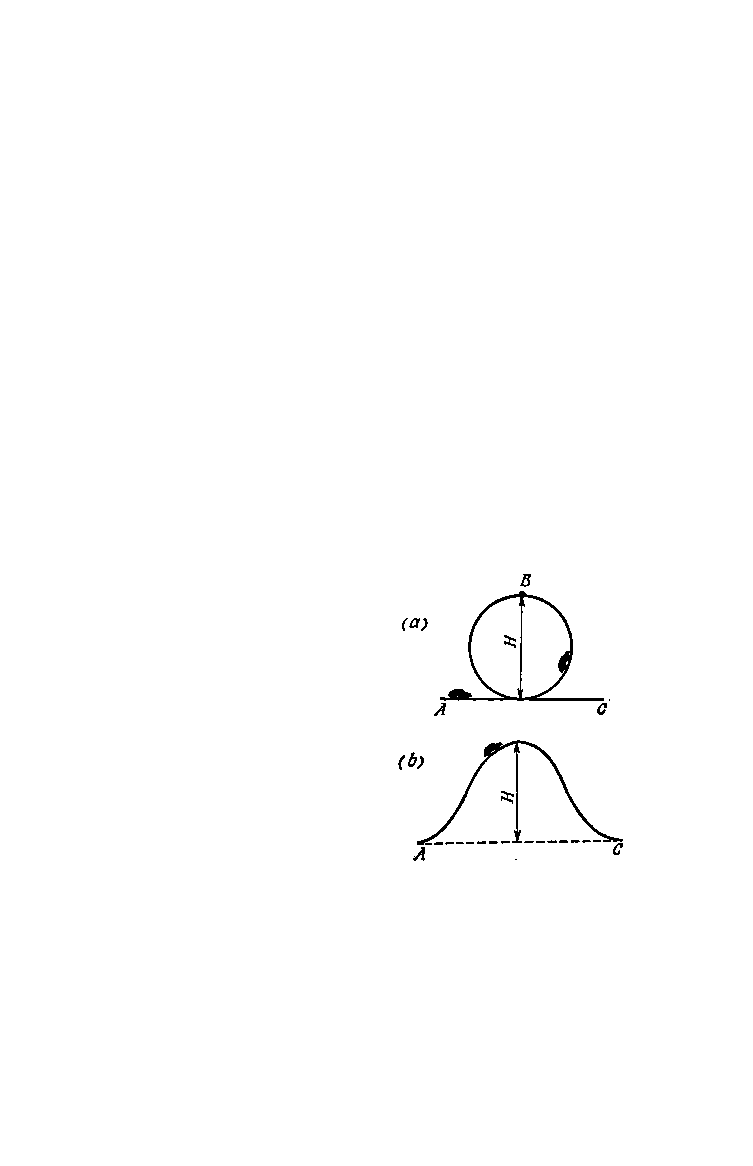
\includegraphics[width=0.6\linewidth]{fig-036a.pdf}
\caption{A body travels from point $A$ to point $C$ via two different paths. The problem is to find the minimum initial velocity in the two cases.}
\label{fig-36}
\end{figure}

\textsc{Student B:} I think that the minimum initial velocity should be the same in both cases, because there is no friction and the same height is to be reached. This velocity can be calculated from the law of conservation of energy
\begin{equation*}
mgH = \frac{mv_{0}^{2}}{2} \, \, \text{from which} \, \, v_{0} = \sqrt{2gH}
\end{equation*}
\\
\textsc{Teacher:} Your answer is wrong. You overlooked the fact that in the first case, the body passes the upper point of its trajectory when it is in a state of rotational motion. This means that at the top point $B$ (\emph{Figure \ref{fig-36} (a)}) it will have a velocity $v_{1}$ determined from a dynamics equation similar to equation (\ref{eq-35}). Since the problem involves the finding of a minimum, we should consider the extreme case when the pressure of the body on its support at point $B$ is reduced to zero. Then only the weight will be acting on the body and imparting to it the centripetal acceleration. Thus
\begin{equation}
mg=\frac{mv_{1}^{2}}{R} = \frac{2mv_{1}^{2}}{H}
\label{eq-39}
\end{equation}
Adding to the dynamics equation (\ref{eq-39}) the energy equation

\begin{equation}
\frac{mv_{0}^{2}}{2} = \frac{mv_{1}^{2}}{2} + mgH
\label{eq-40}
\end{equation}

we find that the minimum initial velocity equals. $\sqrt{\dfrac{5gH}{2}}$. In the second case, the body may pass the top point at a velocity infinitely close to zero and so we can limit ourselves to the energy equation. Then your answer is correct.
\\
\textsc{Student B:} Now I understand. If in the first case the body had no velocity at point $B$, it would simply fall off its track.
\\
\textsc{Teacher:} If in the first case the body had the initial velocity $v_{0}=\sqrt{2gH}$ as you suggested, it would never reach point $B$ but would fall away from the track somewhat earlier. I propose that you find the height $h$ of the point at which the body would fall away from the track if its initial velocity was $v_{0}=\sqrt{2gH}$.
\\
\textsc{Student A:} Please let me try to do this problem.
\\
\textsc{Teacher:} Certainly.
\\
\begin{figure}
\centering
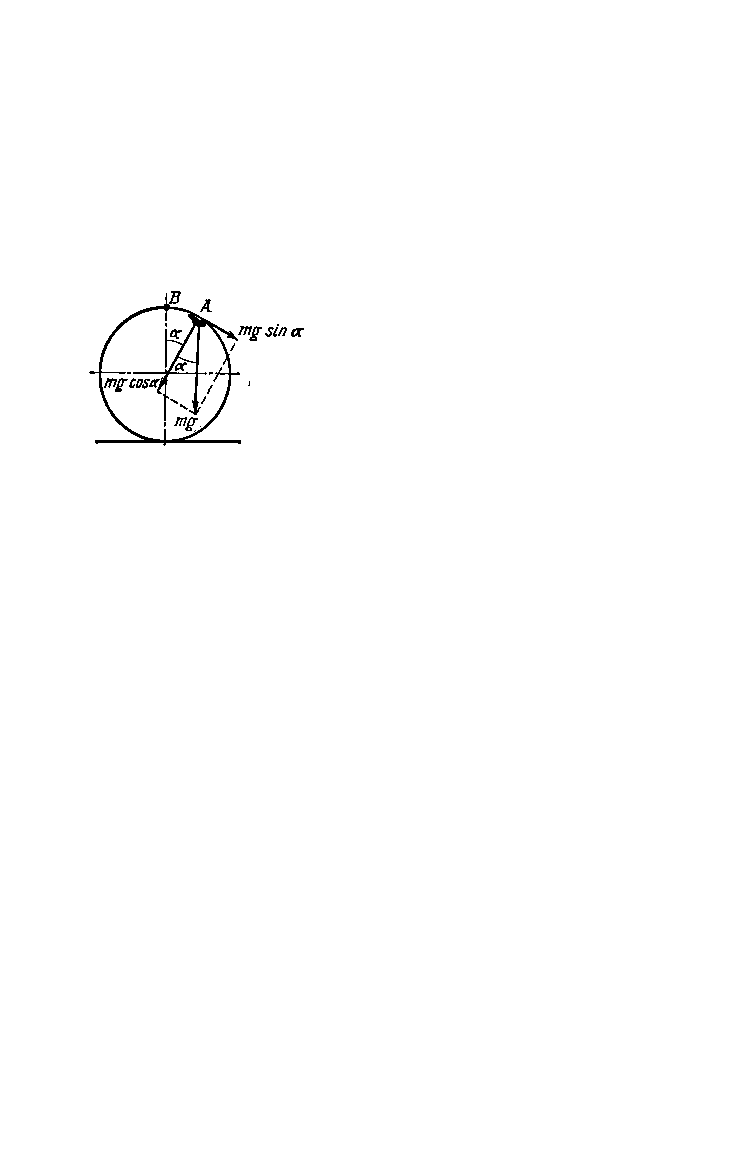
\includegraphics[width=0.6\linewidth]{fig-037a.pdf}
\caption{A on the floor touching a wall at an obtuse angle with the floor.}
\label{fig-37}
\end{figure}
\textsc{Student A:} At the point the body drops off the track the bearing reaction is evidently equal to zero. Therefore, only the weight acts on the body at this point. We can resolve the weight into two components, one along the radius ($mg \cos \alpha$) and the other perpendicular to the radius ($mg \sin \alpha$) as shown in \emph{Figure \ref{fig-37}} (point $A$ is the point at which the body falls away from the track). The component along the radius imparts a centripetal acceleration to the body, determined by the equation
\begin{equation}
mg \cos \alpha = \frac{mv_{2}^{2}}{2}
\label{eq-41}
\end{equation}
where $v_{2}$ is the velocity of the body at point $A$. To find it we can make use of the energy equation
\begin{equation}
\frac{mv_{2}^{2}}{2} + mgh = \frac{mv_{0}^{2}}{2} 
\label{eq-42}
\end{equation}
Combining the dynamics (\ref{eq-41}) and energy (\ref{eq-42}) equations, taking into consideration that 
\begin{equation*}
\cos \alpha = \frac{(h-R)}{R}, \, \, \text{we obtain} \, \, mg(h-R) = mv_{0}^{2} = 2mgh
\end{equation*}
from which
\begin{equation}
h = \frac{2v_{0}^{2}+gH}{6g} 
\label{eq-43}
\end{equation}
After substituting $v_{0}^{2}=2gH$ the final result is
\begin{equation*}
h = \frac{5}{6} H
\end{equation*}
\\
\textsc{Teacher:} Entirely correct. Note that you can use equation (\ref{eq-43}) to find the initial velocity $v_{0}$ for the body to loop the loop. For this we take $h=H$ in equation (\ref{eq-43}). Then
\begin{equation*}
H = \frac{2v_{0}^{2}+gH}{6g} 
\end{equation*}
From this we directly obtain the result previously determined
\begin{equation*}
v_{0} = \sqrt{\frac{5gH}{2}}
\end{equation*}
\\
\textsc{Student A:} Condition (\ref{eq-43}) was obtained for a body falling off its track. How can it be used for the case in which the body loops the loop without falling away?
\\
\textsc{Teacher:} Falling away at the very top point of the loop actually means that the body does not fall away but passes this point, continuing its motion in a circle.
\\
\textsc{Student B:} One could say that the body falls away as if only for a single instant.
\\
\textsc{Teacher:} Quite true. In conclusion I propose the following problem.\\
 \emph{A body lies at the bottom of an inclined plane with an angle of inclination $\alpha$. This plane rotates at uniform angular velocity $\omega$ about a vertical axis. The distance from the body to the axis of rotation of the plane equals $R$. Find the minimum coefficient $k_{0}$ (I remind you that this coefficient characterizes the maximum possible value of the force of static friction) at which the body remains on the rotating inclined plane (\emph{Figure \ref{fig-38}(a)}) without sliding off.}
 \\
 Let us begin as always with the question: what forces are applied to the body?
\\
\begin{marginfigure}[-6cm]
\centering
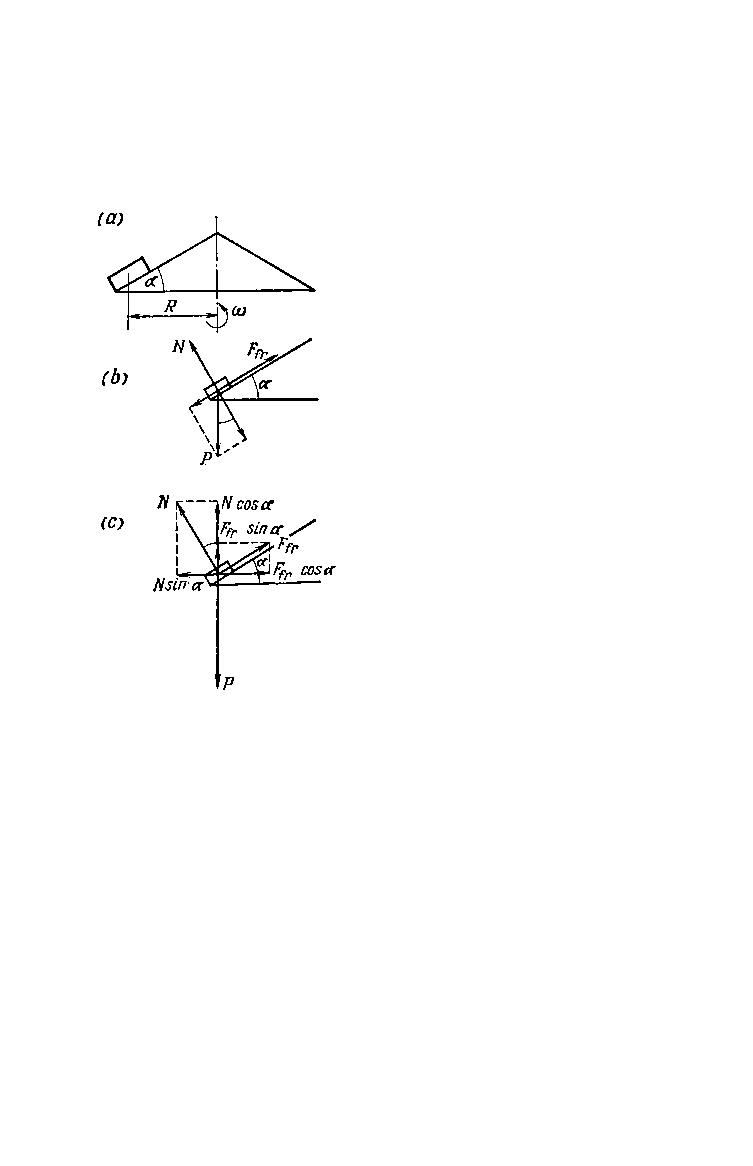
\includegraphics[width=\linewidth]{fig-038a.pdf}
\caption{A body lies on a rotating inclined plane. Problem is to find the maximum value of static friction coefficient at which body remains on the plane without sliding off.}
\label{fig-38}
\end{marginfigure}
\textsc{Student A:} Three forces are applied to the body: the weight $P$, bearing reaction $N$, and the force of friction $F_{fr}$.
\\
\textsc{Teacher:} Quite correct. It's a good thing that you didn't add the centripetal force. Now what are you going to do next?
\\
\textsc{Student A:} Next, I shall resolve the forces in the directions along the plane and perpendicular to it as shown in \emph{Figure \ref{fig-38}(b)}.
\\
\textsc{Teacher:} I'll take the liberty of interrupting you at this point. I don't like the way you have resolved the forces. Tell me, in what direction is the body accelerated?
\\
\textsc{Student A:} The acceleration is directed horizontally. It is centripetal acceleration.
\\
\textsc{Teacher:} Good. That is why you should resolve the forces horizontally (i.e. along the acceleration) and vertically (i.e. perpendicular to the acceleration). Remember what we discussed in  Chapter \ref{ch-06}.
\\
\textsc{Student A:} Now I understand. The resolution of the forces in the horizontal and vertical directions is shown in \emph{Figure \ref{fig-38}(c)}. The vertical components of the forces counterbalance one another, and the horizontal components impart acceleration to the body. Thus
\begin{equation*}
\left.
\begin{aligned}
N \cos \alpha + F_{fr} \sin \alpha = P \\
F_{fr} \cos \alpha -N \sin \alpha = \frac{mv^{2}}{R}
\end{aligned}
\right\}
\end{equation*}
\\
Taking into consideration that 
\begin{equation*}
F_{fr}=k_{0}N, \, \, \left( \frac{v^{2}}{R} \right)=\omega^{2}R \, \, \text{and} \, \, m=\left(\frac{P}{g} \right),
\end{equation*}
\\
we can rewrite these equations in the form
\begin{equation*}
\left.
\begin{aligned}
N (\cos \alpha + k_{0} \sin \alpha)=P \\
N(k_{0} \cos \alpha -\sin \alpha)=P \omega^{2} Rg
\end{aligned}
\right\}
\end{equation*}
\textsc{Student B:} You have only two equations and three unknowns: $k_{0}$, $P$ and $N$.
\\
\textsc{Teacher:} That is no obstacle. We don't have to find all three
unknowns, only the coefficient $k_{0}$ The unknowns $P$ and $N$ can be easily eliminated by dividing the first equation by the second.
\\
\textsc{Student A:} After dividing we obtain
\begin{equation*}
\frac{\cos \alpha+ k_{0} \sin \alpha}{k_{0} \cos \alpha - \sin \alpha} = \frac{g}{\omega^{2}R}
\end{equation*}
\\
which we solve for the required coefficient
\begin{equation}
k_{0} =\left( \frac{\omega^{2}R \cos \alpha+g \sin \alpha}{g \cos \alpha- \omega^{2} R \sin \alpha} \right)
\label{eq-44}
\end{equation}
\\
\textsc{Teacher:} It is evident from equation (\ref{eq-44}) that the condition 
\begin{equation*}
\left( g \cos \alpha- \omega^{2}R \sin \alpha \right) >0
\end{equation*}
should hold true. This condition can also be written in the form
\begin{equation}
\tan \alpha < \frac{g}{\omega^{2}R}
\label{eq-45}
\end{equation}
If condition (\ref{eq-45}) is not complied with, no friction force is capable of retaining the body on the rotating inclined plane.
\\
\section{PROBLEMS}
\begin{enumerate}[resume*=problems]
\item What is the ratio of the forces with which an army tank bears down
on the middle of a convex and of a concave bridge? The radius of curvature
of the bridge is \SI{40}{\metre} in both cases and the speed of the tank is \SI[per-mode=symbol]{45}{\kilo\metre\per\hour}.
\item A body slides without friction from the height $H=\SI{60}{\centi\metre}$ and then loops the
loop of radius $R=\SI{20}{\centi\metre}$ (\emph{Figure \ref{fig-39}}). Find the ratio of the forces with which the body bears against the track at points $A$, $B$ and $C$.
\begin{marginfigure}[-6cm]
\centering
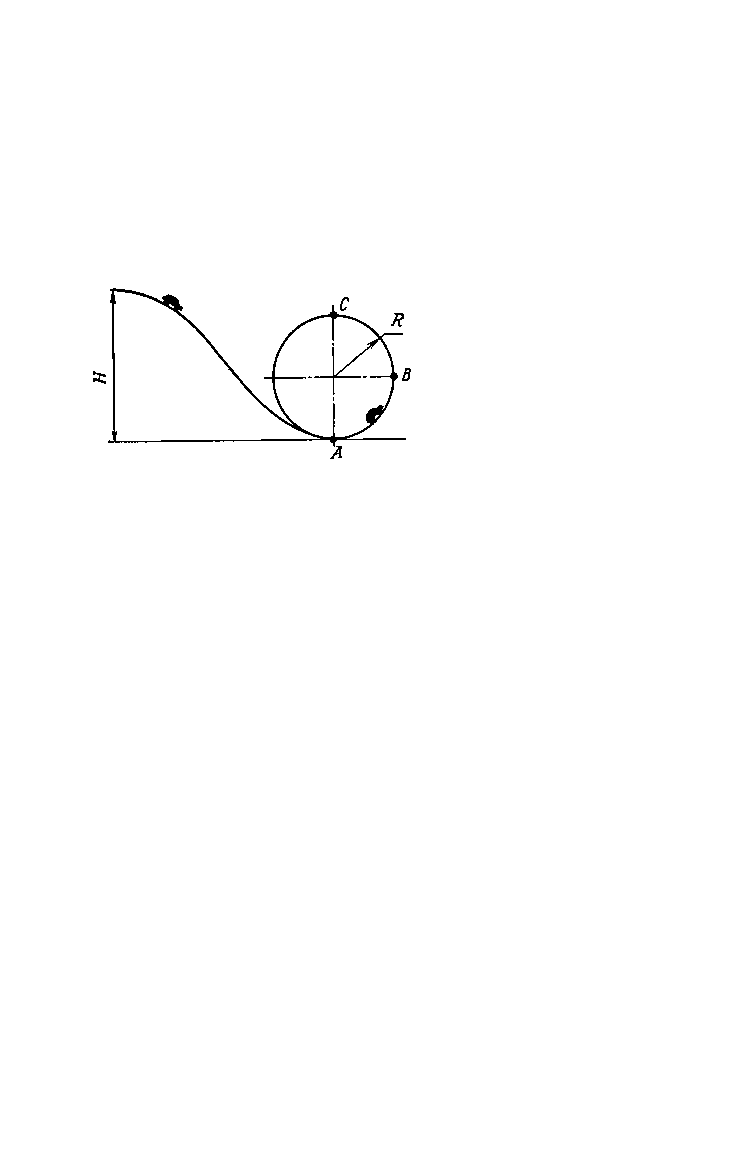
\includegraphics[width=\linewidth]{fig-039a.pdf}
\caption{A body slides from a given height and then loops on a circular track. Problem is to find ratio of forces which the body bears against the track at points $A$, $B$ and $C$. See Problem 16.}
\label{fig-39}
\end{marginfigure}
\item A body can rotate in a vertical plane at the end of a string of length $R$. What horizontal velocity should be imparted to the body in the top position so that the tension of the string in the bottom position is ten times as great as the weight of the body?
\item Calculate the density of the substance of a spherical planet if a satellite rotates about it with a period $T$ in a circular orbit at a distance from the surface of the planet equal to one half of its radius
$R$. The gravitational constant is denoted by $G$.
\item A body of mass $m$ can slide without friction along a trough bent in the form of a circular arc of radiu $R$. At what height $h$ will the body be at rest if the trough rotates at a uniform angular velocity $\omega$ (\emph{Figure \ref{fig-40}}) about a vertical axis? What force $F$ does the body exert on the trough?
\begin{marginfigure}[-6cm]
\centering
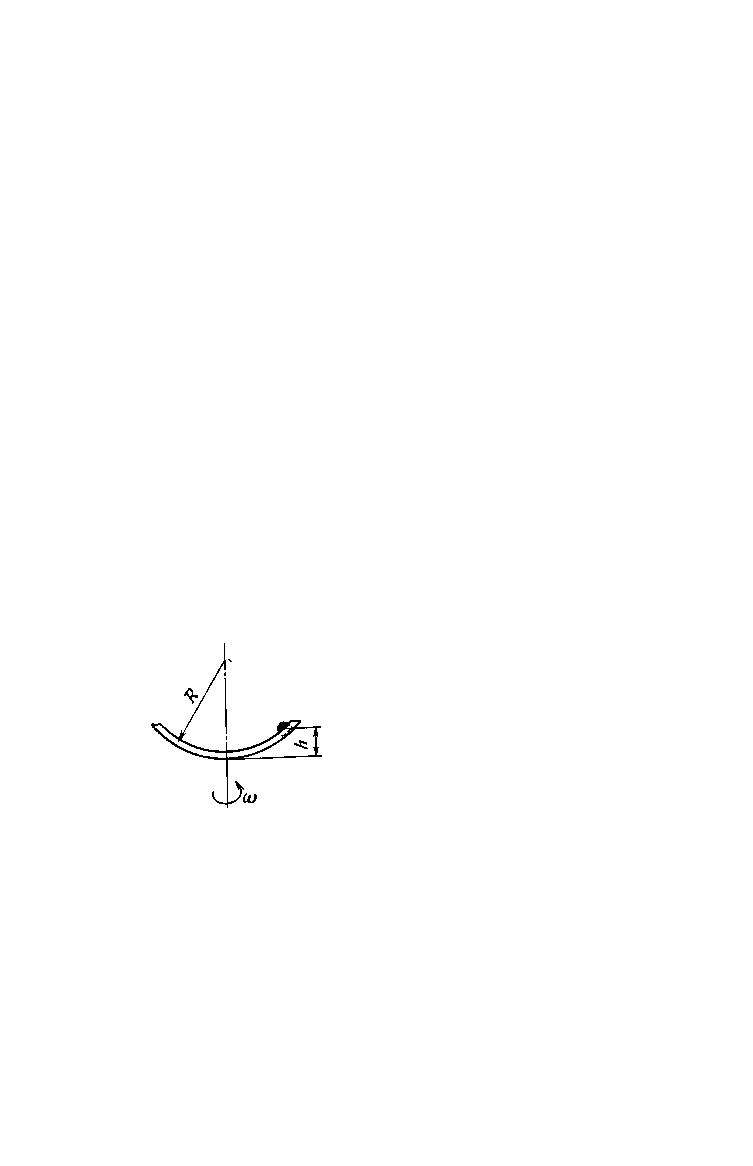
\includegraphics[width=\linewidth]{fig-040a.pdf}
\caption{A body slides without friction on a uniformly rotating circular trough. Problem is to find the force the body exerts on the trough and the height at which the body will be at rest. See Problem 19.}
\label{fig-40}
\end{marginfigure}

\item A hoop of radius R is fixed vertically on the floor. A body slides without friction from the top of the hoop (\emph{Figure \ref{fig-41}}). At what distance $l$ from the point where the hoop is fixed will the body fall?
\begin{marginfigure}[1cm]
\centering
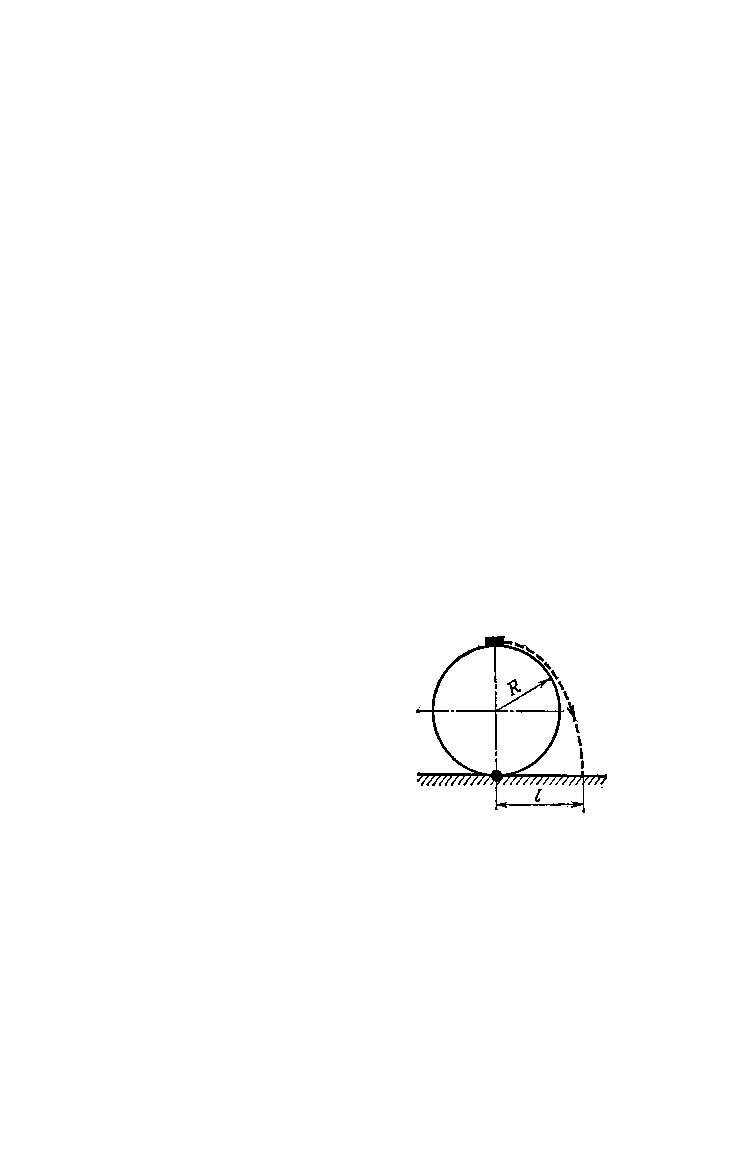
\includegraphics[width=\linewidth]{fig-041a.pdf}
\caption{A body slides without friction form top of the hoop. Problem is to find distance $l$ from the point where the hoop is fixes and the body will fall. See Problem 20.}
\label{fig-41}
\end{marginfigure}

\end{enumerate}

\chapter{How Do You Explain The Weightlessness Of Bodies?}
\label{ch-09}
\paragraph{}
\textsc{Teacher:} How do you understand the expression: ``At the
equator of a planet, a body weightless than at the poles''?
\\
\textsc{Student B:} I understand it as follows. The attraction of a body by the earth is less at the
equator than at the poles for two reasons. In the first place, the earth is somewhat flattened
at the poles and therefore the distance from the centre of the earth is somewhat less to the poles than
to the equator. In the second place, the earth rotates about its axis as a result of which the force
of attraction at the equator is weakened due to the centrifugal effect.
\\
\textsc{Student A:} Please make your last remark a little clearer.
\\
\textsc{Student B:} You must subtract the centrifugal force from the force of attraction.
\\
\textsc{Student A:} I don't agree with you. Firstly, the centrifugal force is not applied to a body travelling in a circle. We already discussed that in the preceding section (Chapter \ref{ch-08}). Secondly,
even if such a force existed it could not prevent the force of attraction from being exactly the same as if there was no rotation of the earth. The force of attraction equals $\dfrac{GmM}{r^{2}}$ and, as such, does not change just because other forces may act on the body.
\\
\textsc{Teacher:} As you can see, the question of the ``weightness of bodies'' is not as simple as it seems at first glance. That's why it is among the questions that examinees quite frequently fail to answer correctly. As a matter of fact, if we agree on the definition that the ``weight of a body'' is the force with which the body is attracted by the earth, i.e, the force $\dfrac{GmM}{r^{2}}$, then the reduction of weight at the equator should be associated only with the flattening at the poles (or bulging
at the equator).
\\
\textsc{Student B:} But you cannot disregard rotation of the earth!
\\
\textsc{Teacher:} I fully agree with you. But first I wish to point out that usually, in everyday life, the ``weight of a body'' is understood to be, not the force with which it is attracted to the earth, and this is quite logical, but the force measured by a spring balance, i. e. the force with which the body bears against the earth. In other words, the bearing reaction is measured (the force with which a body bears against a support is equal to the bearing reaction according to Newton's third
law). It follows that the expression ``a body weighs less at the equator than at the poles'' means that at the equator it bears against its support with a lesser force than at the poles.

Let us denote the force of attraction at the poles by $P_{1}$  and at the equator by $P_{2}$, the bearing reaction at the poles by $N_{1}$ and at the equator by $P_{2}$. At the poles the body is at rest, and at the equator it travels in a circle. Thus
\begin{equation*}
\begin{split}
P_{1} - N_{1} & =0\\
P_{2} - N_{2}& =ma_{cp}
\end{split}
\end{equation*}
\\
where $a_{cp}$ is the centripetal acceleration. We can rewrite these equations in the form
\\
\begin{equation} 
\left.
\begin{split}
N_{1} & = P_{1} \\
N_{2} & = P_{2} - ma_{cp}
\label{eq-46}
\end{split}
\right\}
\end{equation}

Here it is clear that $N_{2}$ is less than $N_{1}$ since, firstly, $P_{2}$ is less than $P_{1}$ (from the effect of the flattening at the poles) and, secondly, we subtract from $P_{2}$ the quantity $ma_{cp}$ (the effect of rotation of the earth).
\\
\textsc{Student B:} So, the expression ``a body has lost half of its weight'' does not mean that the force with which it is attracted to the earth (or any other planet) has been reduced by one half?
\\
\textsc{Teacher:} No, it doesn't. The force of attraction may not change at all. This expression means that the force with which the body bears against its support (in other words, the bearing reaction) has been reduced by one half.
\\
\textsc{Student B:} But then it follows that I can dispose of the ``weightness'' of a body quite freely. What can prevent me from digging a deep pit under the body and letting it fall into the
pit together with its support? In this case, there will be no force whatsoever bearing on the support. Does that mean that the body has completely ``lost its weight''? That it is in a state of weightlessness?
\\
\textsc{Teacher:} You have independently come to the correct conclusion. As a matter of fact, the state of weightlessness is a state of fall of a body. In this connection I wish to make several remarks. I have come across the interpretation of weightlessness as a state in which the force of attraction of
the earth is counterbalanced by some other force. In the case of a satellite, the centrifugal force was suggested as this counterbalancing force. The statement was as follows: 
\\
the force with which the satellite is attracted by the earth and the centrifugal force counter balance each other and, as a result, the resultant force applied to the sateIIite equals zero, and this corresponds to weightlessness.
\\
You now understand, of course, that such a treatment is incorrect if only because no centrifugal force acts on the satellite. Incidentally, if weightlessness is understood to be a state in which the force of attraction is counterbalanced by some other force, then it would be more logical to consider a body weightless when it simply rests on a horizontal plane. This is precisely one of the cases where the weight is counterbalanced by the bearing reaction! Actually, no counter balancing of the force of attraction is required for weightlessness. On the contrary, for a body to become weightless, it is necessary to provide conditions in which no other force acts on it except attraction. In other words, it is necessary that the bearing reaction equal zero. The motion of a body subject to the force of attraction is the falling of the body. Consequently, weightlessness is a state of falling, for example the falling of a lift in a mine shaft or the orbiting of the earth by a satellite.
\\
\textsc{Student A:} In the preceding section (Chapter \ref{ch-08}) you mentioned that the orbiting of a satellite about the earth is none other than its falling to the earth for an indefinitely long period of time.
\\
\textsc{Teacher:} That the motion of a satellite about the earth is falling can be shown very graphically in the following way. Imagine that you are at the top of a high mountain and throw a stone horizontally. We shall neglect the air resistance. The greater the initial velocity of the stone, the farther it will fall. \emph{Figure \ref{fig-42}(a)} illustrates how the trajectory of the stone gradually changes with an increase in the initial velocity. At a certain velocity $v_{1}$ the trajectory of the falling stone becomes a circle and the stone becomes a satellite of the earth. The velocity $v_{1}$ is called the circular orbital velocity. It is found from equation (\ref{eq-34})

\begin{equation} 
%\left.
%\begin{split}
v_{1} = \sqrt{\frac{GM}{r}}
\label{eq-47}
%\end{split}
%\right\}
\end{equation}

If the radius $r$ of the satellite's orbit is taken approximately equal to the radius of the earth then $v_{1} \approx \SI[per-mode=symbol]{8}{\kilo\metre\per\second}$.
\\
\begin{marginfigure}%[-6cm]
\centering
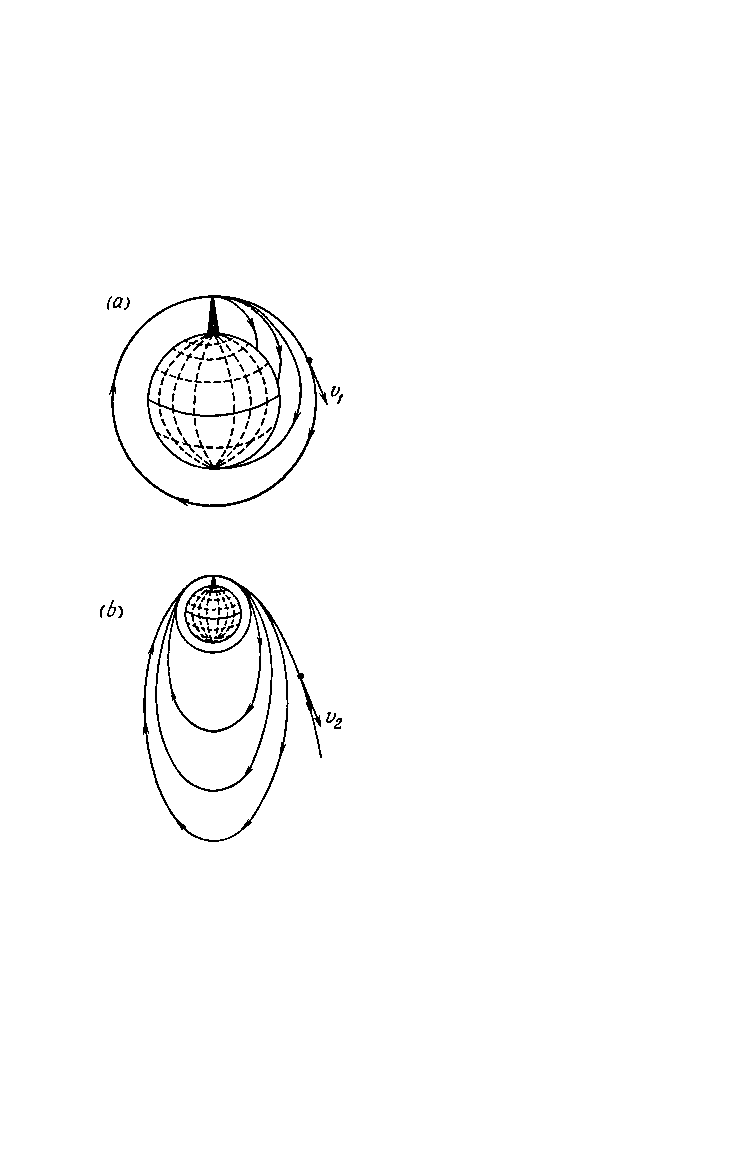
\includegraphics[width=\linewidth]{fig-042a.pdf}
\caption{Trajectory of a body around Earth with different initial velocities.}
\label{fig-42}
\end{marginfigure}


\textsc{Student A:} What will happen if in throwing a stone from
the mountain top we continue to increase the initial velocity?
\\
\textsc{Teacher:} The stone will orbit the earth in a more and more
elongated ellipse (\emph{Figure \ref{fig-42}(b)}). At a certain velocity $v_{2}$ the trajectory of the stone becomes a parabola and the stone ceases to be a satellite of the earth. The velocity $v_{2}$ is called the escape velocity. According to calculations, $v_{2} \approx \SI[per-mode=symbol]{11}{\kilo\metre\per\second}$. This is about $\sqrt{2}$ times $v_{1}$.
\\
\textsc{Student A:} You have defined the state of weightlessness as a state of fall. However, if
the initial velocity of the stone reaches the escape velocity, the stone will leave the earth. In this case, you cannot say that it is falling to the earth. How, then, can you interpret the weightlessness of the stone?
\\
\textsc{Teacher:} Very simply. Weightlessness in this case is the falling of the stone to the sun.
\\
\textsc{Student A:} Then the weightlessness of a spaceship located somewhere in interstellar space is to be associated with the falling of the ship in the gravitational field of some celestial body?
\\
\textsc{Teacher:} Exactly.
\\
\textsc{Student B:} Still, it seems to me that the definition of weightlessness as a state of falling requires some refinement. A parachutist also falls, but he has none of the sensations associated with weightlessness.
\\
\textsc{Teacher:} You are right. Weightlessness is not just any kind of falling. Weightlessness is the so-called free fall, i.e. the motion of a body subject only (!) to the force of gravity. I have already mentioned that for a body to become weightless it is necessary to create conditions under which no other force, except the force of attraction, acts on the body. In the case of the fall of a parachutist, there is an additional force, the resistance of the air.
\\
\section{PROBLEM}
\label{problems-04}

\begin{enumerate}[resume*=problems]
\item Calculate the density of the substance of a spherical planet where the daily period of rotation equals 10 hours, if it is known that bodies are weightless at the equator of the planet.
\end{enumerate}

\cleardoublepage
\thispagestyle{empty}
\vspace*{2cm}

\begin{figure*}
\centering
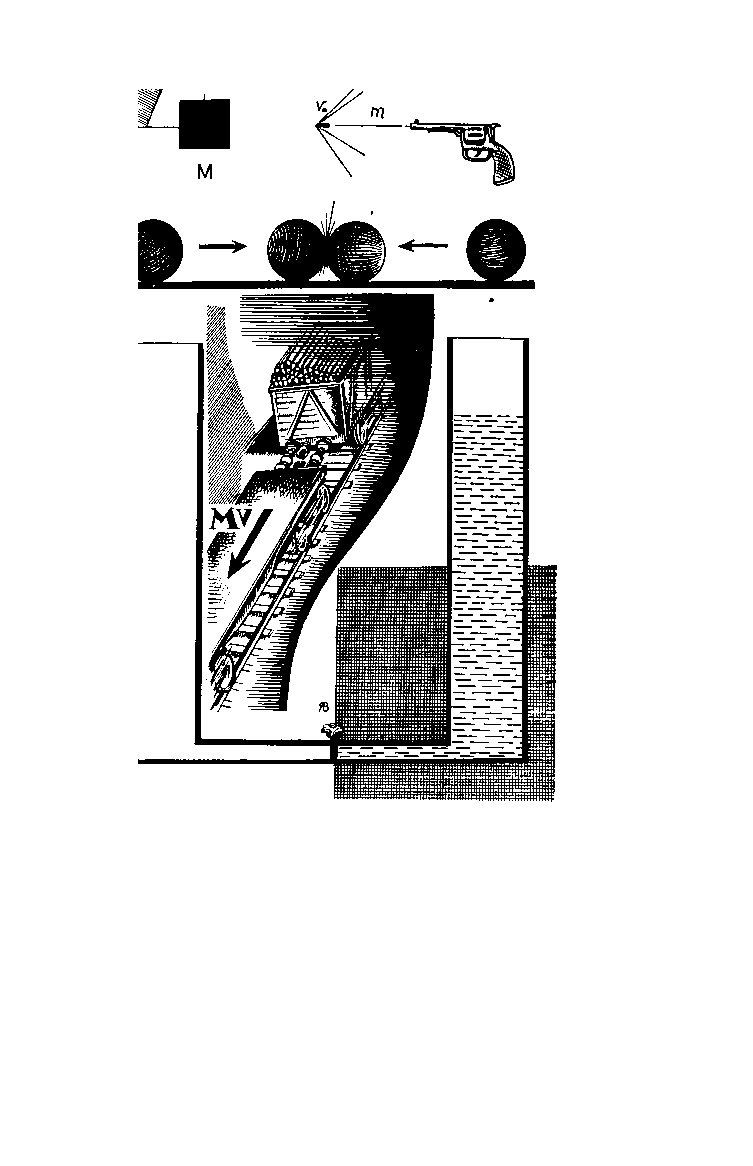
\includegraphics[width=0.65\linewidth]{sec-d.pdf}
%\caption{Velocity \emph{vs} time graph for the function shown in Figure \ref{fig-05}.}
%\label{fig-06}
\end{figure*}
%\addtocounter{figure}{1}
% For incrementing the figure numbers for figures without caption or numbering
\begin{fullwidth}
\begin{Large}
the physical laws of conservation can scarcely be
.ed. They constitute the most general rules estab-
iankind on the basis of the experience of many
. Skillful application of the laws of conservation
ny problems to be solved with comparative ease.
nsider examples concerning the laws of conser-
energy and momentum.
\end{Large}
\end{fullwidth}

\chapter{Can You Apply The Laws Of Conservation Of Energy And Linear Momentum?}
\label{ch-10}
\paragraph{}
\textsc{Teacher:} To begin with I wish to propose several simple problems. 
\begin{description}[leftmargin=1cm, style=nextline]
\item[The first problem:] Bodies slide without friction down two inclined planes of equal height $H$
but with two different angles of inclination $\alpha_{1}$ and $\alpha_{2}$. The initial velocity of the bodies equals zero. Find the velocities of the bodies at the end of their paths.

\item[The second problem:] We know that the formula expressing the final velocity of a body in terms of the acceleration and distance travelled $v = \sqrt{2as}$ refers to the case when there is no initial velocity. What will this formula be if the body has an initial velocity $v_{0}$? 

\item[The third problem:] A body is thrown from a height $H$ with a horizontal velocity of $v_{0}$. Find its velocity when it reaches the ground. 

\item[The fourth problem:] A body is thrown upward at an angle a to the horizontal with an initial velocity $v_{0}$. Find the maximum height reached in its flight.
\end{description}

\textsc{Student A:} I shall solve the first problem in the following way. We first consider one of the inclined planes, for instance the one with the angle of inclination $\alpha_{1}$. Two forces are applied to the body: the force of gravity $P$ and the bearing reaction $N_{1}$. We resolve the force $P$ into two components, one along the plane ($P \sin \alpha_{1}$) and the other perpendicular to it
($P \cos \alpha_{1}$). We then write the equations for the forces perpendicular to the inclined plane
\begin{equation*}
P \cos \alpha_{1} - N_{1} = 0
\end{equation*}
and for the forces along the plane 
\begin{equation*}
P \sin \alpha_{1}  = \frac{P a_{1}}{g}
\end{equation*}
\\
where $a_{1}$ is the acceleration of the body. From the second equation we find that $a_{1} =g \sin \alpha_{1}$. The distance travelled by the body is $\left(\dfrac{H}{\sin \alpha_{1}}\right)$. Next, using the formula mentioned in the second problem, we find that the velocity at the end of
the path is
\begin{equation*}
v_{1}  = \sqrt{a_{1}s_{1}} = \sqrt{\frac{2gH \sin \alpha_{1}}{\sin \alpha_{1}}} = \sqrt{2gH}
\end{equation*}
\\
Since the final result does not depend upon the angle of inclination, it is also applicable to the second plane inclined at the angle $\alpha_{2}$.

To solve the second problem I shall make use of the well known kinematic relationships

\begin{equation*}
\begin{split}
v & = v_{0} + at\\
s & = v_{0}t+ \frac{at^{2}}{2}
\end{split}
\end{equation*}

From the first equation we find that $t= \left(\dfrac{(v - v_{0})}{a}\right)$. Substituting this for $t$ in the second equation we obtain
\begin{equation*}
s = \frac{ v_{0}(v - v_{0})}{a} + \frac{a}{2} \frac{(v - v_{0})^{2}}{a^{2}}
\end{equation*}
or
\begin{equation*}
2sa = 2 v_{0}v - 2v_{0}^{2}+ v^{2} - 2 v_{0}v + v_{0}^{2}
\end{equation*}

from which $2sa=v^{2}-v_{0}^{2}$. The final result is
\begin{equation}
v= \sqrt{2as+v_{0}^{2}}
\label{eq-48}
\end{equation}

To solve the third problem, I shall first find the horizontal $v_{1}$ and vertical $v_{2}$ components of the final velocity. Since the body travels at uniform velocity in the horizontal direction, $v_{1} = v_{0}$. In the vertical direction the body travels with acceleration $g$ but has no initial velocity. Therefore, we can use the formula $v_{2}=\sqrt{2gH}$. Since the sum of the squares of the sides of a right triangle equals, the square of the hypotenuse, the final answer is 
\begin{equation}
v=\sqrt{v_{1}^{2}+v_{2}^{2}} =\sqrt{v_{0}^{2}+2gH}
\label{eq-49}
\end{equation}


The fourth problem has already been discussed in Chapter \ref{ch-05}. It is necessary to resolve the initial velocity into the horizontal ($v_{0} \cos \alpha$) and vertical ($v_{0} \sin \alpha$) components. Then we consider the vertical motion of the body and, first of all, we find the time $t_{1}$ of ascent from the formula for the dependence of the velocity on time in uniformly decelerated motion $(v_{v}=v_{0} \sin \alpha -gt)$, taking into account that at $t=t_{1}$ the vertical velocity of the body vanishes. Thus $v_{0} \sin \alpha -gt_{1} =0$, from which $t_{1} = \left(\dfrac{v_{0}}{g}\right) \sin \alpha$. The time $t_{1}$ being known, we find the height $H$ reached from the formula of the dependence of the distance travelled on time in uniformly decelerated motion. Thus
\begin{equation*}
H = v_{0} t_{1} \sin \alpha - \frac{gt_{1}^{2}}{2} - \left( \frac{v_{0}^{2}}{2g} \right) \sin \alpha
\end{equation*}

\textsc{Teacher:} In all four cases you obtained the correct answers. I am not, however, pleased with the way you solved these problems. They could all have been solved much simpler if you had used the law of conservation of energy. You can see for yourself. 
\begin{description}[leftmargin=1cm, style=nextline]

\item[First problem.] The law of conservation of energy is of the form $mgH = \dfrac{mv^{2}}{2}$ (the potential energy of the body at the top of the inclined plane is equal to its kinetic energy at the bottom). From this equation we readily find the velocity of the body at the bottom
\begin{equation*}
v = \sqrt{2gH}
\end{equation*}


\item[Second problem.] In this case, the law of conservation of energy is of the form 
\begin{equation*}
\frac{mv_{0}^{2}}{2}+mas= \frac{mv^{2}}{2}, 
\end{equation*}

where $mas$ is the work done by the forces in imparting the acceleration $a$ to the body. This leads immediately to $v_{0}^{2} + 2as = v_{2}$ or, finally, to 

\begin{equation*}
v=\sqrt{2as+v_{0}^{2}}
\end{equation*}

\item[Third problem.] We write the law of conservation of energy as 
\begin{equation*}
mgH+\frac{mv_{0}^{2}}{2}= \frac{mv^{2}}{2}.
\end{equation*}

Then the result is

\begin{equation*}
v=\sqrt{2gH+v_{0}^{2}}
\end{equation*}

\item[Fourth problem.] At the point the body is thrown its energy equals $\dfrac{mv_{0}^{2}}{2}$. At the top point of its trajectory, the energy of the body is $mgH+\dfrac{mv_{1}^{2}}{2}$. Since the velocity $v_{1}$ at the top point equals $v_{0} \cos \alpha$, then, using the law of conservation of energy

\begin{equation*}
\frac{mv_{0}^{2}}{2} = mgH + \frac{mv_{0}^{2}}{2} \cos^{2} \alpha
\end{equation*}

we find that

\begin{equation*}
H=\left(\frac{v_{0}^{2}}{2g} \right) \left( 1 - \cos^{2} \alpha \right)
\end{equation*}

or, finally

\begin{equation*}
H=\left(\frac{v_{0}^{2}}{2g} \right) \sin^{2} \alpha 
\end{equation*}

\end{description}

\textsc{Student A:} Yes, it's quite clear to me that these problems can be solved in a much simpler way. It didn't occur to me to use the law of conservation of energy.
\\
\textsc{Teacher:} Unfortunately, examinees frequently forget about this law. As a result they begin to solve such problems by more cumbersome methods, thus increasing the probability of errors. My advice is: make more resourceful and extensive use of the law of conservation of energy. This poses the question: how skillfully can you employ this law?
\\
\textsc{Student A:} It seems to me that no special skill is required; the law of conservation of energy as such is quite simple.
\\
\textsc{Teacher:} The ability to apply a physical law correctly is not determined by its complexity or simplicity. Consider a example. Assume that a body travels at uniform velocity in a circle in a horizontal plane. No friction forces operate. The body is subject to a centripetal force. What is the work done
by this force in one revolution of the body?
\\
\textsc{Student A:} Work is equal to the product of the force by the distance through which it acts. Thus, in our case, it equals 

\begin{equation*}
\left(\frac{mv^{2}}{R}\right) 2 \pi R = 2nmv^{2}, 
\end{equation*}

where $R$ is the radius of the circle and $m$ and $v$ are the mass and velocity of the body.
\\
\textsc{Teacher:} According to the law of conservation of energy; work cannot completely disappear. What has become of the work you calculated?
\\
\textsc{Student A:} It has been used to rotate the body.
\\
\textsc{Teacher:} I don't understand. State it more precisely.
\\
\textsc{Student A:} It keeps the body on the circle.
\\
\textsc{Teacher:} Your reasoning is wrong. No work at all is required to keep the body on the circle.
\\
\textsc{Student A:} Then I don't know how to answer your question.
\\
\textsc{Teacher:} Energy imparted to a body can be distributed, as physicists say, among the following ``channels'':
\begin{enumerate}[label=(\arabic*),leftmargin=1.5cm] 
\item Increasing the kinetic energy of the body; 
\item Increasing its potential energy; 
\item Work performed by the given body on other bodies; and 
\item Heat evolved due to friction. 
\end{enumerate}

Such is the general principle which not all examinees understand with sufficient clarity. Now consider the work of the centripetal force. The body travels at a constant velocity and therefore its kinetic energy
is not increased. Thus the first channel is closed. The body travels in a horizontal plane and, consequently, its potential energy is not changed. The second channel is also closed. The given body does not perform any work on other bodies, so that the third channel is closed. Finally, all kinds of friction have been excluded. This closes the fourth and last channel.
\\
\textsc{Student A:} But then there is simply no room for the work of the centripetal force, or is there?
\\
\textsc{Teacher:} As you see, none. It remains now for you to declare your position on the matter. Either you admit that the law your this your of conservation of energy is not valid, and then all troubles are gone, or you proceed from the validity of law and then \ldots{}. However, try to find the way out of
difficulties.
\\
\textsc{Student A:} I think that it remains to conclude that the centripetal force performs no work whatsoever.
\\
\textsc{Teacher:} That is quite a logical conclusion. I want to point out that' it is the direct consequence of the law of conservation of energy.
\\
\textsc{Student B:} All this is very well, but what do we do about the formula for the work done by a body?
\\
\textsc{Teacher:} In addition to the force and the distance through which it acts, this formula should also contain the cosine of fa) the angle between the direction of the force and the velocity

\begin{equation*}
A = F s \cos \alpha
\end{equation*}

In the given case, $\cos \alpha = 0$.
\\
\textsc{Student A:} Oh yes, I entirely forgot about this cosine.
\\
\textsc{Teacher:} I want to propose another example. Consider communicating vessels connected by a narrow tube with a stopcock. Assume that at first all the liquid is in the left vessel and its height is $H$ (\emph{Figure \ref{fig-43}(a)}). Then we open the stopcock and the liquid flows from the left into the right vessel. The flow ceases when there is an equal level of $\dfrac{H}{2}$ in each vessel (\emph{Figure \ref{fig-43}(b)}).

Let us calculate the potential energy of the liquid in the initial and final positions. For this we multiply the weight of the liquid in each vessel by one half of the column of liquid. In the initial position the potential energy equalled $\dfrac{PH}{2}$, and in the final one it is 

\begin{equation*}
 \left( \frac{P}{2} \right)  \left( \frac{H}{4} \right) +  \left( \frac{P}{2} \right)   \left( \frac{H}{4} \right) =   \left( \frac{PH}{4} \right).
\end{equation*}


\begin{marginfigure}
\centering
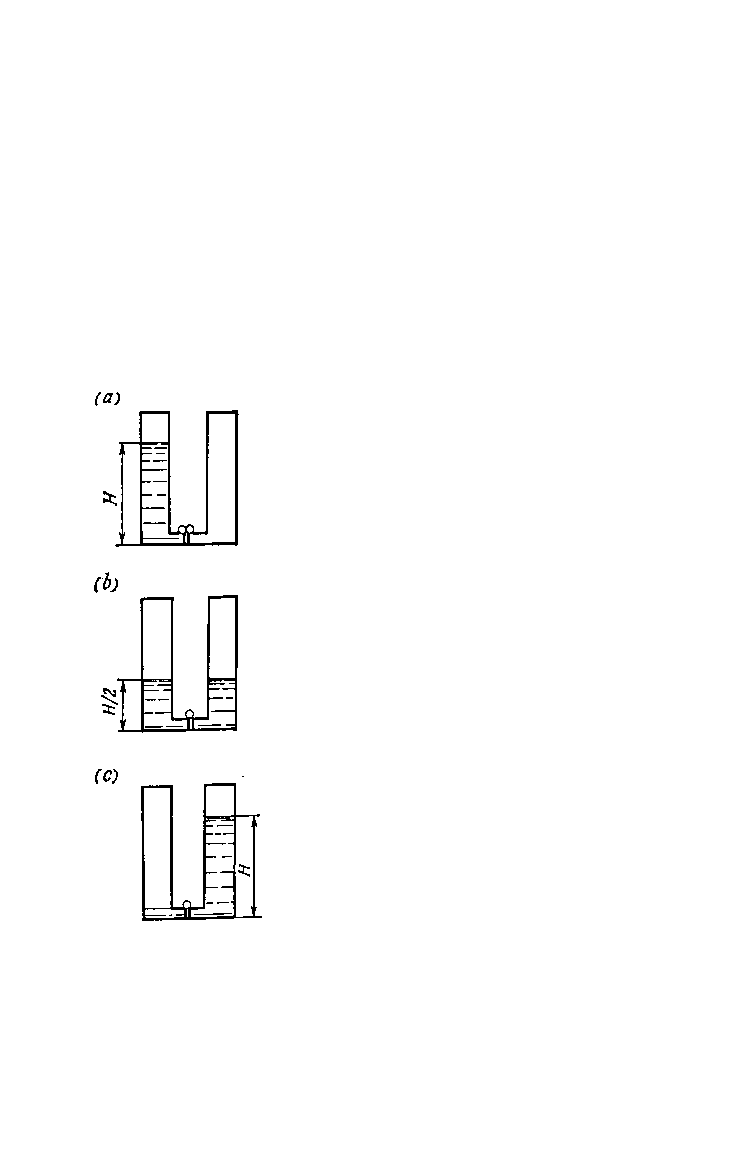
\includegraphics[width=0.8\linewidth]{fig-043a.pdf}
\caption{A body travels from point $A$ to point $C$ via two different paths. The problem is to find the minimum initial velocity in the two cases.}
\label{fig-43}
\end{marginfigure}

Thus in the final state, the potential energy of the liquid turns out to be only one half of that in the
initial state. Where has one half of the energy disappeared to?
\\
\textsc{Student A:} I shall attempt to reason as you advised. The potential energy $\dfrac{PH}{4} $ could be used up in performing work on other bodies, on heat evolved in friction and on the kinetic energy of the liquid itself. Is that right?
\\
\textsc{Teacher:} Quite correct. Continue.
\\
\textsc{Student A:} In our case, the liquid flowing from one vessel to the other does not perform any work on other bodies. The liquid has no kinetic energy in the final state because it is in a state of rest. Then, it remains to conclude that one half of the potential energy has been converted into heat
evolved in friction. True, I don't have a very clear idea of what kind of friction it is.
\\
\textsc{Teacher:} You reasoned correctly and came to the right conclusion. I want to add a few words on the nature of friction. One can imagine that the liquid is divided into layers, each characterizing a definite rate of flow. The closer the layer to the walls of the tube, the lower its velocity. There is an exchange of molecules between the layers, as a result of which molecules with a higher velocity of ordered motion find themselves among molecules with a lower velocity of ordered
motion, and vice versa. As a result, the ``faster'' layer has an accelerating effect on the ``slower'' layer and, conversely, the ``slower'' layer has a decelerating effect on the ``faster'' layer.

This picture allows us to speak of the existence of a peculiar internal friction between the layers. Its effect is stronger with a greater difference in the velocities of the layers in the middle part of the tube and near the walls. Note that the velocity of the layers near the walls is influenced by the kind of inter-
action between the molecules of the liquid and those of the walls. If the liquid wets the tube then the layer directly adjacent to the wall is actually stationary.
\\
\textsc{Student A:} Does this mean that in the final state the temperature of the liquid should be somewhat higher than in the initial state?
\\
\textsc{Teacher:} Yes, exactly so. Now we shall change the conditions of the problem to some extent. Assume that there is no interaction between the liquid and the tube walls. Hence, all the layers will flow at the same velocity and there will be no internal friction. How then will the liquid flow from one
vessel to the other?
\\
\textsc{Student A:} Here the potential energy will be reduced owing to the kinetic energy acquired by the liquid. In other words, the state illustrated in \emph{Figure \ref{fig-43}(b)} is not one of rest. The liquid will continue to flow from the left vessel to the right one until it reaches the state shown in \emph{Figure \ref{fig-43}(c)}. In this state the potential energy is again the same as in the initial state \emph{Figure \ref{fig-43}(a)}.
\\
\textsc{Teacher:} What will happen to the liquid after this?
\\
\textsc{Student A:} The liquid will begin to flow back in the reverse direction, from the right vessel to the left one. As a result, the levels of the liquid will fluctuate in the communicating vessels.
\\
\textsc{Teacher:} Such fluctuations can be observed, for instance, in communicating glass vessels containing mercury. We know that mercury does not wet glass. Of course these fluctuations will be damped in the course of time, since it is impossible to completely exclude the interaction between the
molecules of the liquid and those of the tube walls.
\\
\textsc{Student A:} I see that the law of conservation of energy can be applied quite actively.
\\
\textsc{Teacher:} Here is another problem for you. \\
\emph{A bullet of mass $m$, travelling horizontally with a velocity $v_{0}$, hits a wooden block of mass $M$, suspended on a string, and sticks in the block. To what height $H$ will the block rise, after the bullet hits it, due to deviation of the string from the equilibrium position (\emph{Figure \ref{fig-44}})?}
\\
\begin{figure}
\centering
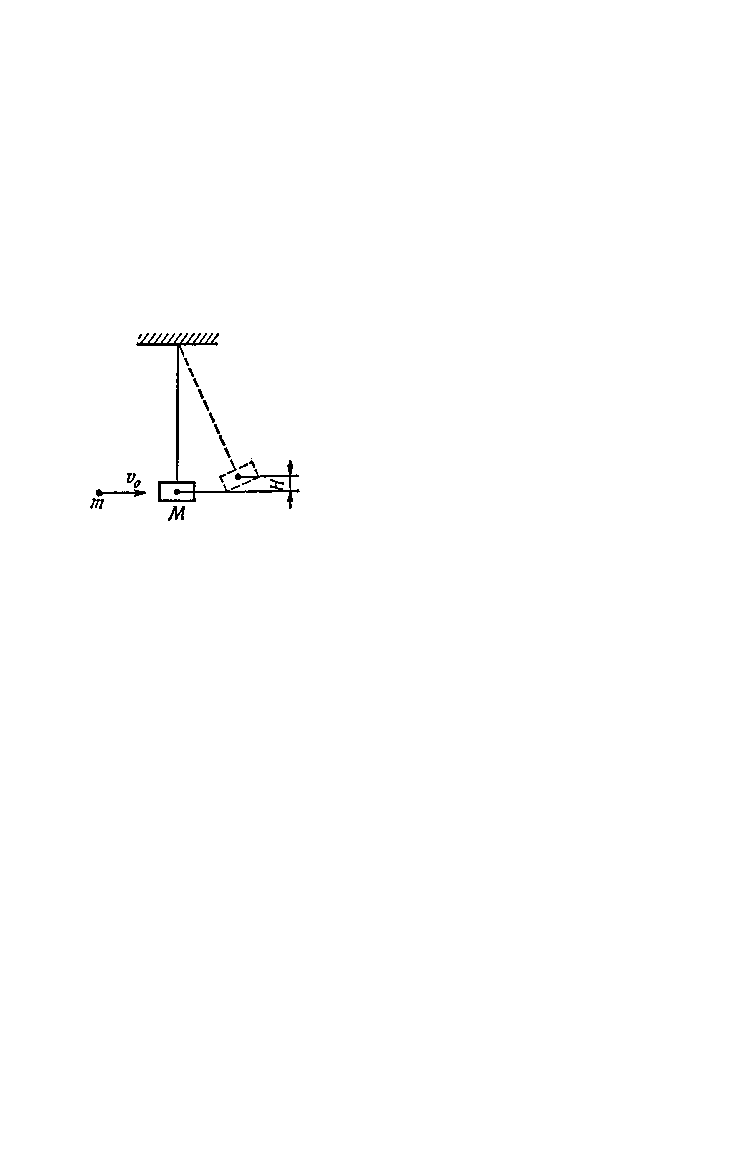
\includegraphics[width=0.4\linewidth]{fig-044a.pdf}
\caption{A bullet hits a block of wood and sticks in it. Problem is to find the height to which the block will rise after the impact.}
\label{fig-44}
\end{figure}

\textsc{Student A:} We shall denote by $v_{1}$ the velocity of the block with the bullet immediately after the bullet hits the block. To find this velocity we make use of the law of conservation of energy. Thus
\\
\begin{equation}
\frac{m v_{o}^{2}}{2} = \left( m + M \right) \frac{v_{1}^{2}}{2}
\label{eq-50}
\end{equation}
from which
\begin{equation}
v_{1} = v_{o} \sqrt{\frac{m}{ m + M}} 
\label{eq-51}
\end{equation}

This velocity being known, we find the sought-for height $H$ by again resorting to the law of conservation of energy
\\
\begin{equation}
(m+ M) gH = (m + M) 	\frac{v_{1}^{2}}{2}
\label{eq-52}
\end{equation}

Equations (\ref{eq-50}) and (\ref{eq-52}) can be combined
\\
\begin{equation*}
(m+ M) gH = \frac{mv_{0}^{2}}{2}
\end{equation*}

from which \\
\begin{equation}
H = \frac{m}{(m + M)} 	\frac{v_{0}^{2}}{2g}
\label{eq-53}
\end{equation}
\textsc{Teacher:} (to Student B): What do you think of this solution?
\\
\textsc{Student B:} I don't agree with it. We were told previously that in such cases the law of conservation of momentum is to be used. Therefore, instead of equation (\ref{eq-50}) I would have used
a different relationship 
\\
\begin{equation}
mv_{0} = (m+M) v_{1}
\label{eq-54}
\end{equation}
(the momentum of the bullet before it hits the block is equal to the momentum of the bullet and block afterward). From this it follows that
\\
\begin{equation}
v_{1} = v_{0} \frac{m}{(m + M)}
\label{eq-55}
\end{equation}

If we now use the law of conservation of energy (\ref{eq-52}) and substitute the result of equation (\ref{eq-55}) into (\ref{eq-52}) we obtain
\\
\begin{equation}
H = \left(\frac{m}{m + M} \right)^{2}	\frac{v_{0}^{2}}{2g}
\label{eq-56}
\end{equation}
\textsc{Teacher:} We have two different opinions and two results. The point is that in one case the law of conservation of kinetic energy is applied when the bullet strikes the block, and in the other case, the law of conservation of momentum. Which is correct? (to Student A): What can you say to justify your
position?
\\
\textsc{Student A:} It didn't occur to me to use the law of conservation of momentum.
\\
\textsc{Teacher:} (to Student B): And what do you say?
\\
\textsc{Student B:} I don't know how to substantiate my position. I remember that in dealing with collisions, the law of conservation of momentum is always valid, while the law of conservation of energy does not always hold good. Since in the given case these laws lead to different results, my solution is evidently correct.
\\
\textsc{Teacher:} As a matter of fact, it is indeed quite correct. It is, however, necessary to get a better insight into the matter. A collision after which the colliding bodies travel stuck together (or one inside the other) is said to be a ``completely inelastic collision''. Typical of such impacts is the presence of permanent set in the colliding bodies, as a result of which a certain amount of heat is evolved. Therefore, equation (\ref{eq-50}), referring only to the kinetic energy of bodies, is inapplicable. In our case, it is necessary to employ the law of conservation of momentum (\ref{eq-54}) to find the velocity of the box with the bullet after the impact.
\\
\textsc{Student A:} Do you mean to say that the law of conservation of energy is not valid for a completely inelastic collision? But this law is universal.
\\
\textsc{Teacher:} There is no question but that the law of conservation of energy is valid for a completely inelastic collision as well. The kinetic energy is not conserved after such a collision. I specifically mean the kinetic energy and not the whole energy. Denoting the heat evolved in collision by $Q$, we can write the following system of laws of conservation referring to the completely inelastic collision discussed above \\
\begin{equation} 
\left.
\begin{split}
mv_{0}^{2}  & = v_{1} {m + M}\\
\frac{mv_{0}^{2}}{2} & = \frac{(m+M) v_{1}^{2}}{2} + Q
\label{eq-57}
\end{split}
\right\}
\end{equation}

Here the first equation is the law of conservation of momentum, and the second is the law of conservation of energy (including not only mechanical energy, but heat as well). The system of equations (\ref{eq-57}) contains two unknowns: $v_{1}$ and $Q$. After determining $v_{1}$ from the first equation, we can use the second equation to find the evolved heat $Q$
\\
\begin{equation} 
%\left.
%\begin{split}
Q = \frac{mv_{0}^{2}}{2} - \frac{(m+M)m^{2}v_{0}^{2}}{2(m+M)^{2}} =  \frac{mv_{0}^{2}}{2} \left( 1 - \frac{m}{m+M}\right)
\label{eq-58}
%\end{split}
%\right\}
\end{equation}
It is evident from this equation that the larger the mass $M$, the more energy is converted into heat. In the limit, for an infinitely large mass. $M$, we obtain $Q=\frac{m v_{0}^{2}}{2}$, i.e, all the
kinetic energy is converted into heat. This is quite natural: assume that the bullet sticks in a wall.
\\
\textsc{Student A:} Can there be an impact in which no heat is evolved?
\\
\textsc{Teacher:} Yes, such collisions are possible. They are said to be ``perfectly elastic''. For instance, the impact of two steel balls can be regarded as perfectly elastic with a fair degree of approximation. Purely elastic deformation of the balls occurs and no heat is evolved. After the collision, the balls return to their original shape.
\\
\textsc{Student A:} You mean that in a perfectly elastic collision, the law of conservation of energy becomes the law of conservation of kinetic energy?
\\
\textsc{Teacher:} Yes, of course.
\\
\textsc{Student A:} But in this case I cannot understand how you can reconcile the laws of conservation of momentum and of energy. We obtain two entirely different equations for the velocity after impact. Or, maybe, the law of conservation of momentum is not valid for a perfectly elastic collision.
\\
\textsc{Teacher:} Both conservation laws are valid for a perfectly elastic impact: for momentum and for kinetic energy. You have no reason to worry about the reconciliation of these laws because after a perfectly elastic impact, the bodies fly apart at different velocities. Whereas after a completely inelastic
impact the colliding bodies travel at the same velocity (since they stick together), after an elastic impact each body travels at its own definite velocity. Two unknowns require two equations. 

Let us consider an example. Assume that a body of mass $m$ travelling at a velocity $v_{0}$ elastically collides with a body of mass $M$ at rest. Further assume that as a result of the impact the incident body bounces back. We shall denote the velocity of body m after the collision by $v_{1}$ and that of body $M$ by $v_{2}$. Then the laws of conservation of momentum and energy can be written in the form\\
\begin{equation} 
\left.
\begin{split}
mv_{0} & =Mv_{2}-  mv_{1} \\
\frac{mv_{0}^{2}}{2} & = \frac{mv_{2}^{2}}{2} + \frac{mv_{1}^{2}}{2}
\label{eq-59}
\end{split}
\right\}
\end{equation}

Note the minus sign in the first equation. It is due to our assumption that the incident body bounces back.
\\
\textsc{Student B:} But you cannot always know beforehand in which direction a body will. travel after the impact. Is it impossible for the body m to continue travelling in the same direction but at a lower velocity after the collision?
\\
\textsc{Teacher:} That is quite possible. In such a case, we shall obtain a negative velocity $v_{1}$ when solving the system of equations (\ref{eq-59}).
\\
\textsc{Student B:} I think that the direction of travel of body $m$ after the collision is determined by the ratio of the masses $m$ and $M$.
\\
\textsc{Teacher:} Exactly. If $m<M$, body $m$ will bounce back; at $m=M$, it will be at rest after the collision; and at $m>M$, it will continue its travel in the same direction but at a lower velocity. In the general case, however, you need not worry about the direction of travel. It will be sufficient to assume
some direction and begin the calculations. The sign of the answer will indicate your mistake, if any.
\\
\textsc{Student B:} We know that upon collision the balls may fly apart at an angle to each other. We assumed that motion takes place along a single straight line. Evidently, this must have been a special case.
\\
\textsc{Teacher:} You' are right. We considered what is called a central collision in which the balls travel before and after the impact along a line passing through their centres. The more general case of the off-centre collision will be dealt with later. For the time being, I'd like to know if everything is quite clear.
\\
\textsc{Student A:} I think I understand now. As I see it, in any collision (elastic or inelastic), two laws of conservation are applicable: of momentum and of energy. Simply the different nature of the impacts leads to different equations for describing the conservation laws. In dealing with inelastic collisions,
it is necessary to take into account the heat evolved on impact.
\\
\textsc{Teacher:} Your remarks are true and to the point.
\\
\textsc{Student B:} So far as I understand it, completely elastic and perfectly inelastic collisions are the two extreme cases. Are they always suitable for describing real cases?
\\
\textsc{Teacher:} You are right in bringing up this matter. The cases of collision we have considered are extreme ones. In real collisions some amount of heat is always generated (no ideally elastic deformation exists) and the colliding bodies may fly apart with different velocities. In many cases, however, real
collisions are described quite well by means of simplified models: completely elastic and perfectly inelastic collisions.

Now let us consider an example of an off-centre elastic collision. 

\emph{A body in the form of an inclined plane with a \ang{45} angle of inclination lies on a horizontal plane. A ball of mass $m$, flying horizontally with a velocity $v_{0}$, collides with the body (inclined plane), which has a mass of $M$. As a result of the impact, the ball bounces vertically upward and the body $M$ begins to slide without friction along the horizontal plane. Find the velocity with which the ball begins its vertical travel after the collision (Fig. 45).}

Which of you wishes to try your hand at this problem?
\\

\begin{figure}
\centering
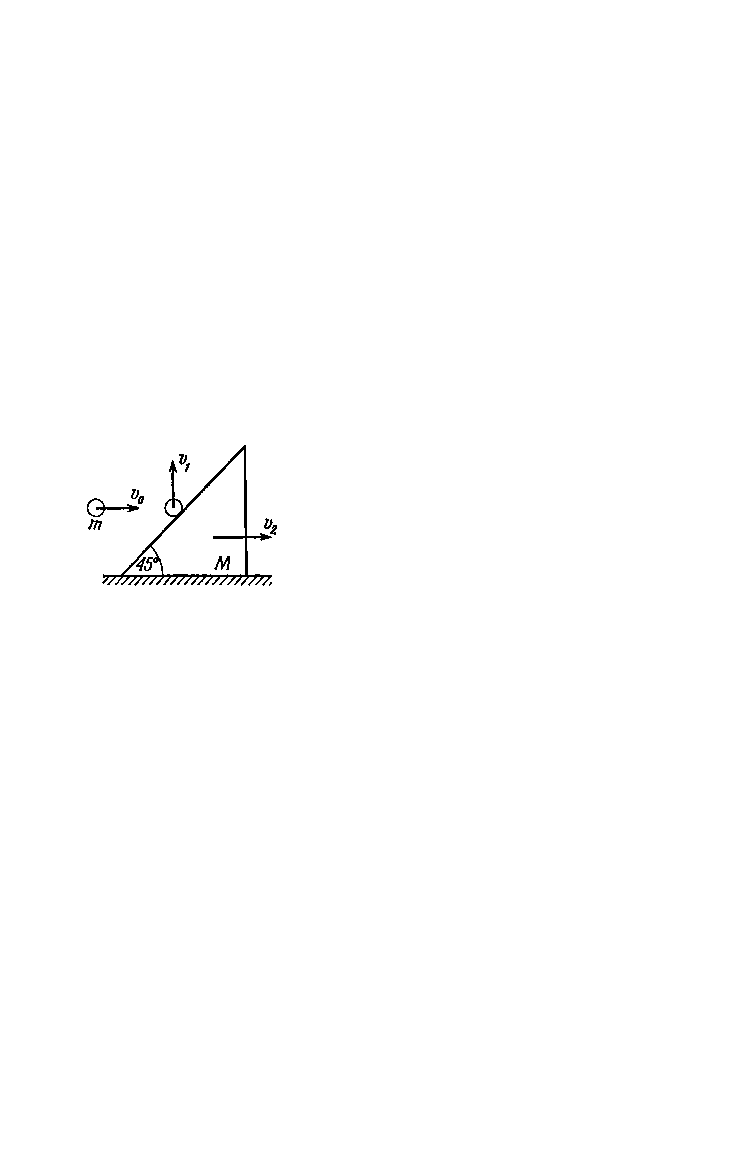
\includegraphics[width=0.4\linewidth]{fig-045a.pdf}
\caption{A ball collides with another body at rest on the inclined plane. The problem is to find the velocity of the ball after the impact.}
\label{fig-45}
\end{figure}

\textsc{Student B:} Allow me to. Let us denote the sought-for velocity of the ball by $v_{1}$ and that of body $M$ by $v_{2}$. Since the collision is elastic, I have the right to assume that the kinetic energy is conserved. Thus
\\
\begin{equation} 
%\left.
%\begin{split}
%mv_{0} & =Mv_{2}-  mv_{1} \\
\frac{mv_{0}^{2}}{2} = \frac{mv_{1}^{2}}{2} + \frac{mv_{2}^{2}}{2} 
\label{eq-60}
%\end{split}
%\right\}
\end{equation}

I need one more equation, for which I should evidently use the law of conservation of momentum. I shall write it in the form 
\begin{equation} 
%\left.
%\begin{split}
mv_{0} =Mv_{2} +  mv_{1} 
\label{eq-61}
%\end{split}
%\right\}
\end{equation}

True, I'm not so sure about this last equation because velocity $v_{1} $ is at right angles to velocity $v_{2}$.
\\
\textsc{Teacher:} Equation (\ref{eq-60}) is correct. Equation (\ref{eq-61}) is incorrect, just as you thought. You should remember that the law of conservation of momentum is a vector equation, since the momentum is a vector quantity having the same direction as the velocity. True enough, when all the velocities are directed along a single straight line, the vector equation can be replaced by a scalar one. That is precisely what happened when we discussed central collisions. In the general case, however, it is
necessary to resolve all velocities in mutually perpendicular directions and to write the law of conservation of momentum for each of these directions separately (if the problem is considered in a plane, the vector equation can be replaced by two scalar equations for the projections of the momentum in the two mutually perpendicular directions).

For the given problem we can choose the horizontal and vertical directions. For the horizontal direction, the law of conservation of momentum is of the form

\begin{equation}
mv_{0}= Mv_{2}
\label{eq-62}
\end{equation}

From equations (\ref{eq-60}) and (\ref{eq-62}) we find the velocity
\begin{equation*}
v_{1} = \sqrt{\frac{M-m}{m}}
%\label{eq-62}
\end{equation*}
\textsc{Student B:} What do we do about the vertical direction?
\\
\textsc{Teacher:} At first sight, it would seem that the law of conservation of momentum is not valid for the vertical direction. Actually it is. Before the impact there were no vertical velocities; after the impact, there is a momentum $mv_{1}$, directed vertically upwards. We can readily see that still another body participates in the problem: the earth. If it was not for the earth, body $M$ would not travel horizontally
after the collision. Let us denote the mass of the earth by $M_{\Earth}$ and the velocity it acquires as a result of the impact by $v_{\Earth}$.

The absence of friction enables us to treat the interaction between the body $M$ and the earth as taking place only in the vertical direction. In other words, the velocity $v_{\Earth}$ of the earth is directed vertically downwards. Thus, the participation of the earth in our problem doesn't change the form of equation (\ref{eq-62}), but leads to an equation which describes the law of conservation of momentum for the vertical direction
\begin{equation} 
%\left.
%\begin{split}
mv_{1}  - M_{e}v_{e} = 0   
\label{eq-63}
%\end{split}
%\right\}
\end{equation}
\\
\textsc{Student B:} Since the earth also participates in this problem it will evidently be necessary to correct the energy relation (\ref{eq-60}).
\\
\textsc{Teacher:} Just what do you propose to do to equation (\ref{eq-60})?
\\
\textsc{Student B:} I wish to add a term concerning the motion of the earth after the impact
\\
\begin{equation} 
%\left.
%\begin{split}
%mv_{0} & =Mv_{2}-  mv_{1} \\
\frac{mv_{0}^{2}}{2} = \frac{mv_{1}^{2}}{2} + \frac{Mv_{2}^{2}}{2} +  \frac{M_{\Earth}v_{\Earth}^{2}}{2} 
\label{eq-64}
%\end{split}
%\right\}
\end{equation}

\textsc{Teacher:} Your intention is quite logical. There is, however, no need to change equation (\ref{eq-60}). As a matter of fact, it follows from equation (\ref{eq-63}) that the velocity of the earth is
\\
\begin{equation*}
v_{e} = \frac{mv_{1}}{M_{\Earth}}
\end{equation*}

Since the mass $M_{\Earth}$ is practically infinitely large, the velocity $v_{\Earth}$ of the earth after the impact is practically equal to zero. Now, let us rewrite the term $\dfrac{M_{e}v_{e}^{2}}{2} $ in equation (\ref{eq-64}) to obtain the form $\dfrac{(M_{\Earth}v_{\Earth})v_{\Earth}}{2}$. The quantity $M_{\Earth}v_{\Earth}$ in this product has, according to equation (\ref{eq-63}), a finite value. If this value is multiplied by zero (in the given case by $v_{\Earth}$) the product is also zero. From this we can conclude that the earth participates very peculiarly in this problem. It acquires a certain momentum, but at the same time, receives practically no energy. In other words, it participates in the law of conservation of momentum, but does not participate in the law of conservation of energy. Th is circumstance is especially striking evidence of the fact that the laws of conservation of energy and of momentum are essentially different, mutually independent laws.
\\
\section{PROBLEMS}
\label{problems-05}

\begin{enumerate}[resume*=problems]
\item A body with a mass of \SI{3}{\kilogram} falls from a certain height with an initial velocity of \SI{2}[per-mode=symbol]{\meter\per\second}, directed vertically downward. Find the work done to overcome the forces of resistance during \SI{10}{\second} if it is known that the body acquired a velocity of \SI{50}[per-mode=symbol]{\meter\per\second} at the end of the \SI{10}{\second} interval. Assume that the force of resistance is constant.

\item A body slides first down an inclined plane at an angle of \ang{30} and then along a horizontal surface. Determine the coefficient of friction if it is known that the body slides along the horizontal surface the same distance as along the inclined plane.

\item Calculate the efficiency of an inclined plane for the case when a body slides off it at uniform velocity.

\item A ball of mass $m$ and volume $V$ drops into water from a height $H$, plunges to a depth $h$ and then jumps out of the water (the density of the ball is less than that of water). Find the resistance of the water (assuming it to be constant) and the height $h_{1}$ to which the ball ascends after jumping
out of the water. Neglect air resistance. The density of water is denoted by $\rho_{w}$.

\item A railway car with a mass of 50 tons, travelling with a velocity of \SI[per-mode=symbol]{12}{\kilo\meter\per\hour}, runs into a flatcar with a mass of 30 tons standing on the same track. Find the velocity of joint travel of the railway car and flatcar directly after the automatic coupling device operates. Calculate the distance travelled by the two cars after being coupled if the force of resistance is 5 per cent of the weight.

\item A cannon of mass $M$, located at the base of an inclined plane, shoots a shell of mass $m$ in a horizontal direction with an initial velocity $v_{0}$. To what height does the cannon ascend the inclined plane as a result of recoil if the angle of inclination of the plane is $\alpha$ and the coefficient of friction between the cannon and the plane is $k$?

\item Two balls of masses $M$ and $2M$ are hanging on threads of length $l$ fixed at the same point. The ball of mass $M$ is pulled to one side through an angle of $\alpha$ and is released after imparting to it a tangential velocity of $v_{0}$ in the direction of the equilibrium position. To what height will the balls rise after collision if: 
\begin{enumerate}
\item the impact is perfectly elastic, and
\item if it is completely inelastic (the balls stick together as a result of the impact)?
\end{enumerate}


\item A ball of mass $M$ hangs on a string of length $l$. A bullet of mass $m$, flying horizontally, hits the ball and sticks in it. At what minimum velocity must the bullet travel so that the ball will make one complete revolution in a vertical plane?

\item Two wedges with angles of inclination equal to \ang{45} and each of mass $M$ lie on a horizontal plane (\emph{Figure \ref{46}}). A ball of mass $m$ ($m \ll M$) drops freely from the height $H$. It first strikes one wedge and then the other and bounces vertically upward. Find the height to which the ball bounces. Assume that both impacts are elastic and that there is no friction between the wedges and the plane.
\begin{marginfigure}
\centering
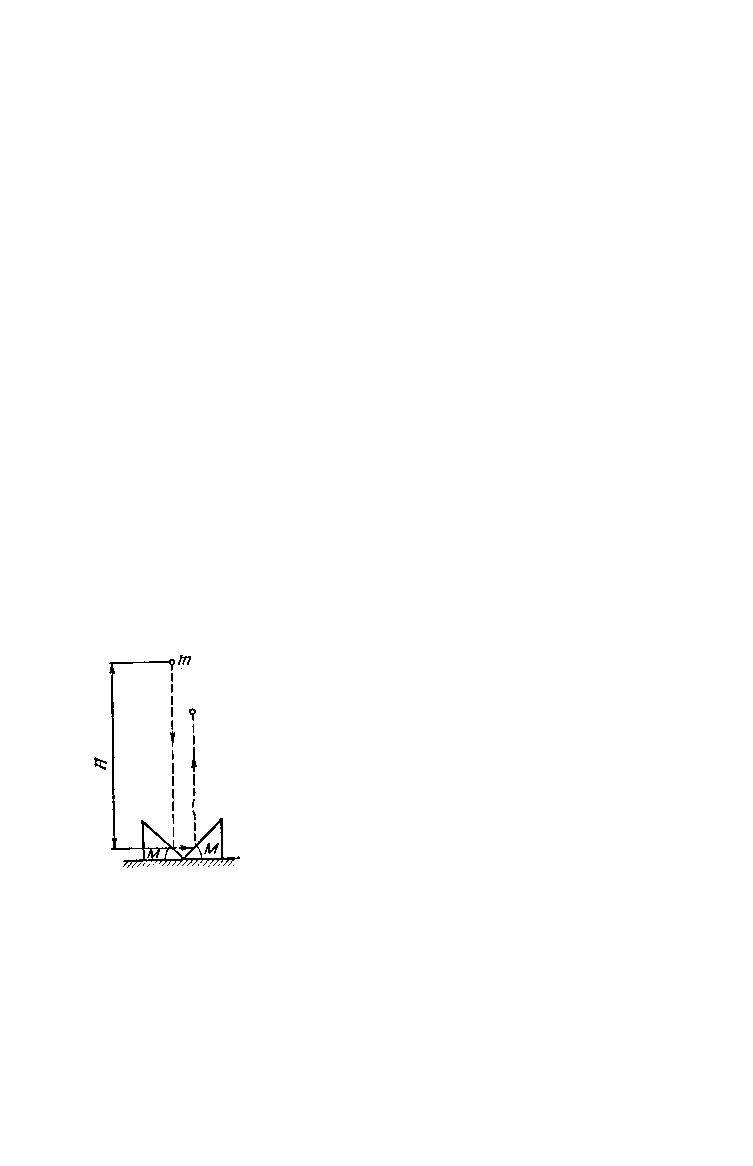
\includegraphics[width=0.8\linewidth]{fig-046a.pdf}
\caption{A ball strikes ones of the two edges after being dropped from a height. First it strikes the second wedge and then goes vertically up. The problem is to find the height to which the ball rises.}
\label{fig-46}
\end{marginfigure}

\item A wedge with an angle of \ang{30} and a mass $M$ lies on a horizontal plane. A ball of mass $m$ drops freely from the height $H$, strikes the wedge elastically and bounces away at an angle of \ang{30} to the horizontal. To what height does the ball ascend? Neglect friction between the wedge and the horizontal plane.\end{enumerate}

\cleardoublepage
\thispagestyle{empty}
\vspace*{2cm}

\begin{figure*}
\centering
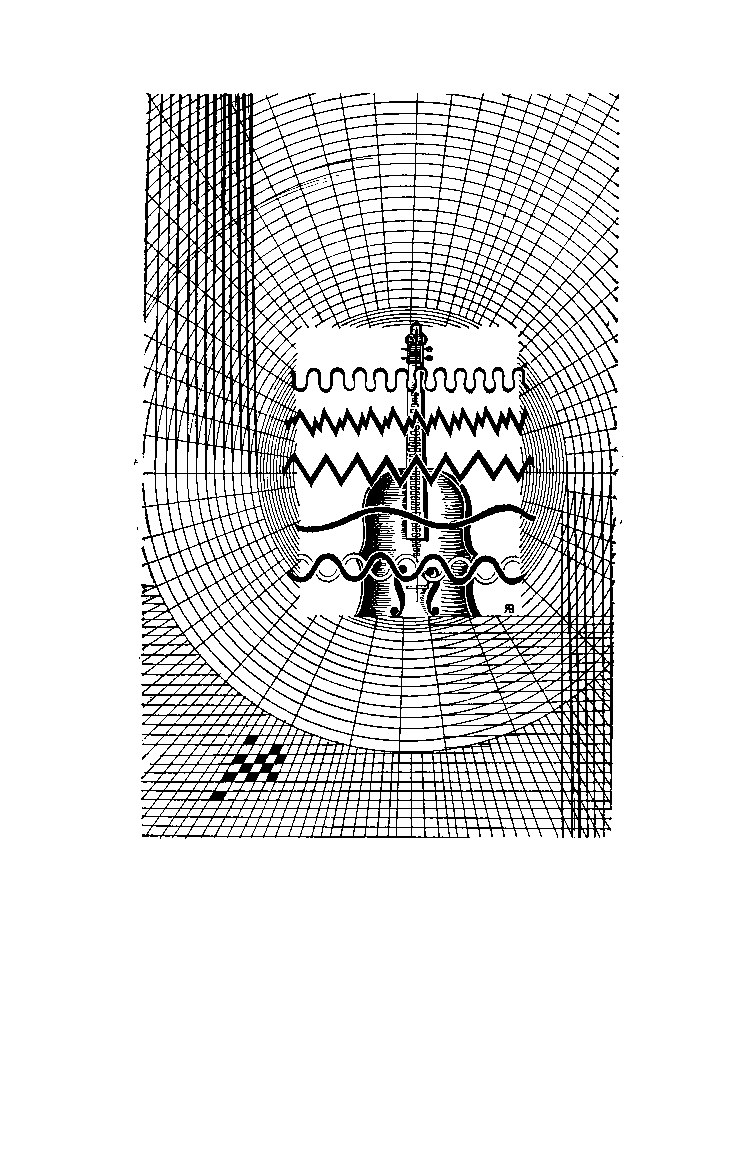
\includegraphics[width=0.65\linewidth]{sec-e.pdf}
%\caption{Velocity \emph{vs} time graph for the function shown in Figure \ref{fig-05}.}
%\label{fig-06}
\end{figure*}
%\addtocounter{figure}{1}
% For incrementing the figure numbers for figures without caption or numbering
\begin{fullwidth}
\begin{Large}
The world about us is full of vibrations and waves. Remember this when you study the branch of physical science devoted to these phenomena. 
\\
Let us discuss harmonic vibrations and, as a special case, the vibrations of a mathematical pendulum. We shall analyse the behaviour of the pendulum in non-inertial frames of reference.
\end{Large}
\end{fullwidth}

\chapter{Can You Deal With Harmonic Vibrations?}
\label{ch-11}

\textsc{Teacher:} Some examinees do not have a sufficiently clear
understanding of harmonic vibrations. First let us discuss their definition.
\\
\textsc{Student A:} Vibrations are said to be harmonic if they obey the sine law: the deviation $x$ of a body from its equilibrium position varies with time as follows
\begin{equation}
x= A \sin ( \omega t + a)
\label{eq-65}
\end{equation}

where $A$ is the amplitude of vibration (maximum deviation of the body from the position of
equilibrium), $\omega$ is the circular frequency ($\omega = 2 \pi T$, where $T$ is the period of vibration), and $\alpha$ is the initial phase (it indicates the deviation of the body from the position of equilibrium at the instant of time $t=0$). The idea of harmonic vibrations is conveyed by the motion of the projection of a point which rotates at uniform angular velocity $\omega$ in a circle of radius $A$
\\
\begin{marginfigure}
\centering
\includegraphics[width=0.8\linewidth]{fig-047a.pdf}
\caption{Simple harmonic motion and its relations.}
\label{fig-47}
\end{marginfigure}

\textsc{Student B:} I prefer another definition of harmonic vibrations. As is known, vibrations occur due to action of the restoring force, i.e. a force directed toward the position of equilibrium and increasing as the body recedes from the equilibrium position. Harmonic vibrations are those in which the restoring force $F$ is proportional to the deviation $x$ of the body from the equilibrium position. Thus\\
\begin{equation}
F=kx
\label{eq-66}
\end{equation}
Such a force is said to be ``elastic''.
\\
\textsc{Teacher:} I am fully satisfied with both proposed definitions. In the first case, harmonic vibrations are defined on the basis of how they occur; in the second case, on the basis of their cause. In other words, the first definition uses the space-time (kinematic) description of the vibrations, and the
second, the causal (dynamic) description.
\\
\textsc{Student B:} But which of the two definitions is preferable? Or, maybe, they are equivalent?
\\
\textsc{Teacher:} No, they are not equivalent, and the first (kinematic) is preferable. It is more complete.
\\
\textsc{Student B:} But whatever the nature of the restoring force, it will evidently determine the nature of the vibrations. I don't understand, then, why my definition is less complete.
\\
\textsc{Teacher:} This is not quite so. The nature of the restoring force does not fully determine the nature of the vibrations.
\\
\textsc{Student A:} Apparently, now is the time to recall that the nature of the motion of a body at a given instant is determined not only by the forces acting on the body at the given instant, but by the initial conditions as well, i.e. the position and velocity of the body at the initial instant. We discussed
this in  Chapter \ref{ch-04}.
\\
\textsc{Teacher:} Absolutely correct. With reference to the case being considered this statement means that the nature of the vibrations is determined not only by the restoring force, but by the conditions under which these vibrations started. It is evident that vibrations can be effected in various ways. For
example, a body can be deflected a certain distance from its equilibrium position and then smoothly released. It will begin to vibrate. If the beginning of vibration is taken as the zero instant, then from equation (\ref{eq-65}), we obtain $\alpha=\dfrac{\pi}{2}$, and the distance the body is deflected is the amplitude of vibration. The body can be deflected different distances from the equilibrium position, thereby setting different amplitudes of vibration.

Another method of starting vibrations is toImpart a certain initial velocity (by pushing) to a body in a state of equilibrium. The body will begin to vibrate. Taking the beginning of vibration as the zero point, we obtain from equation (\ref{eq-65}) that $\alpha=0$. The amplitude of these vibrations depends
upon the initial velocity imparted to the body. It is evidently possible to propose innumerable other, intermediate methods of exciting vibrations. For instance, a body is deflected from its position of equilibrium and, at the same time, is pushed or plucked, etc. Each of these methods will set de-
finite values of the amplitude $A$ and the initial phase $\alpha$ of the vibration.
\\
\textsc{Student B:} Do you mean that the quantities $A$ and $\alpha$ do not depend upon the nature of the restoring force?
\\
\textsc{Teacher:} Exactly. You manipulate these two quantities at your own discretion when you excite vibrations by one or another method. The restoring force, i. e. coefficient $k$ in equation (\ref{eq-66}), determines only the circular frequency $\omega$ or, in other words, the period of vibration of the body. It can be said that the period of vibration is an intrinsic characteristic of the vibrating body, while the amplitude $A$ and the initial phase $\alpha$ depend upon the external conditions that excite the given vibration.

Returning to the definitions of harmonic vibrations, we see that the dynamic definition contains no information on either the amplitude or initial phase. The kinematic definition, on the contrary , contains information on these quantities.
\\
\textsc{Student B:} But if we have such a free hand in dealing with the amplitude, maybe it is not so important a characteristic of a vibrating body?
\\
\textsc{Teacher:} You are mistaken. The amplitude is a very important characteristic of a vibrating body. To prove this, let us consider an example. A ball of mass $m$ is attached to two elastic springs and accomplishes harmonic vibrations of amplitude $A$ in the horizontal direction (\emph{Figure \ref{fig-48}}). The restoring force is determined by the coefficient of elasticity $k$ which characterizes the elastic properties of the springs. Find the energy of the vibrating ball.
\begin{marginfigure}
\centering
\includegraphics[width=0.8\linewidth]{fig-048a.pdf}
\caption{Simple harmonic motion and its relations.}
\label{fig-48}
\end{marginfigure}

%Fig. 49
\textsc{Student A:} To find the energy of the ball, we can consider its position of extreme deflection ($x = A$). In this position, the velocity of the ball equals zero and therefore its total energy is its potential energy. The latter can be determined as the work done against the restoring force $F$ in displacing the
ball the distance $A$ from its equilibrium position. Thus
\\
\begin{equation}
W = FA
\label{eq-67}
\end{equation}
Next, taking into account that $F=kA$, according to equation (\ref{eq-66}), we obtain
\\
\begin{equation*}
W=kA^{2}
\end{equation*}

\begin{marginfigure}
\centering
\includegraphics[width=0.8\linewidth]{fig-049a.pdf}
\caption{Force varying with distance.}
\label{fig-49}
\end{marginfigure}
\textsc{Teacher:} You reasoned along the proper lines, but committed an error. Equation (\ref{eq-67}) is applicable only on condition that the force is constant. In the given case, force $F$ varies with the distance, as shown in \emph{Figure \ref{fig-49}}. The work done by this force over the distance $x=A$ is equal to the hatched area under the force curve. This is the area of a triangle and is equal to
$\dfrac{kA^{2}}{2}$. Thus\\
\begin{equation}
W = \frac{kA^{2}}{2}
\label{eq-68}
\end{equation}

Note that the total energy of a vibrating body is proportional to the square of the amplitude of vibration. This demonstrates what an important characteristic of a vibrating body the amplitude is.
If $0 < x < A$, then the total energy $W$ is the sum of two components-the kinetic and potential energies \\
\begin{equation}
W = \frac{kA^{2}}{2} = \frac{m v^{2}}{2} + \frac{k x^{2}}{2}
\label{eq-69}
\end{equation}

Equation (\ref{eq-69}) enables the velocity $v$ of the vibrating ball to be found at any distance $x$ from the equilibrium position. My next question is: what is the period of vibration of the ball shown in \emph{Figure \ref{fig-48}}?
\\
\textsc{Student B:} To establish the formula for the period of vibration it will be necessary to employ differential calculus.
\\
\textsc{Teacher:} Strictly speaking, you are right. However, if we simultaneously use the kinematic and dynamic definitions of harmonic vibrations we can manage without differential calculus. As a matter of fact, we can' conclude from \emph{Figure \ref{fig-47}}, which is a graphical expression of the kinematic definition, that the velocity of the body at the instant it passes the equilibrium position is \\
\begin{equation}
v_{1} = \omega A =  \frac{2 \pi A}{T}
\label{eq-70}
\end{equation}

Using the result of equation (\ref{eq-68}), following from the dynamic definition, we can conclude that velocity $v_{1}$ can be found from the energy relation \\
\begin{equation}
\frac{m v_{1}^{2}}{2} + \frac{k A^{2}}{2}
\label{eq-71}
\end{equation}
(at the instant the ball passes the equilibrium position the entire energy of the ball is kinetic energy). Combining equations (\ref{eq-70}) and (\ref{eq-71}), we obtain 
\\
\begin{equation*}
\frac{4 \pi^{2} A^{2} m}{T^{2}}=kA^{2}, 
\end{equation*}
from which\\
\begin{equation}
T=2 \pi \sqrt{\frac{m}{k}}
\label{eq-72}
\end{equation}
As mentioned previously, the period of vibration is determined fully by the properties of the vibrating system itself, and is independent of the way the vibrations are set up.
\\
\textsc{Student A:} When speaking of vibrations we usually deal, not with a ball attached to springs,
but with a pendulum. Can the obtained results be generalized to include the pendulum?
\\
\textsc{Teacher:} For such generalization we must first find out what, in the case of the pendulum, plays the role of the coefficient of elasticity $k$. It is evident that a pendulum vibrates not due to an elastic force, but to the force of gravity. Let us consider a ball (called a bob in a pendulum) suspended on a string of length $l$. We pull the bob to one side of the equilibrium position so that the string makes an angle $\alpha$, (\emph{Figure \ref{fig-50}}) with the vertical. Two forces act on the bob: the force of gravity $mg$ and the tension $T$ of the string. Their resultant is the restoring force. As is evident from the figure, it equals $mg \sin \alpha$.\\

\begin{marginfigure}
\centering
\includegraphics[width=\linewidth]{fig-050a.pdf}
\caption{Anaysing the motion of a pendulum.}
\label{fig-50}
\end{marginfigure}
\textsc{Student A:} Which of the lengths, $\overline{AB}$ or $\overline{AC}$, should be considered the deflection of the pendulum from the equilibrium position (see \emph{Figure \ref{fig-50}})? .
\\
\textsc{Teacher:} We are analysing the harmonic vibrations of a pendulum. For this it is necessary that the angle of maximum deviation of the string from the equilibrium position be very small \\
\begin{equation}
\alpha \ll 1
\label{eq-73}
\end{equation}

(note that here angle $\alpha$ is expressed in radians; in degrees, angle $\alpha$ should, in any case, be less than \ang{10}). If condition (\ref{eq-73}) is complied with, the difference between the lengths $\overline{AB}$ and $\overline{AC}$ can be neglected \\
\begin{equation*}
\overline{AB} = l \sin \alpha \approx \overline{AC} = l \tan \alpha
\end{equation*}

Thus your question becomes insignificant. For definiteness, we can assume that $x = \overline{AB}=l \sin \alpha$. Then equation (\ref{eq-66}) will take the following form for a pendulum \\
\begin{equation}
mg \sin \alpha = k l \sin \alpha
\tag{66a}
\label{eq-66a}
\end{equation}

from which\\

\begin{equation}
k= \frac{mg}{l}
\label{eq-74}
\end{equation}

Substituting this equation into equation (\ref{eq-72}), we obtain the formula for the period of harmonic vibrations of a pendulum
\\
\begin{equation}
T=2 \pi \sqrt{\frac{l}{g}}
\label{eq-75}
\end{equation}

We shall also take up the question of the energy of the pendulum. Its total energy is evidently equal to $mgh$, where $h$ is the height to which the bob ascends at the extreme position (see \emph{Figure \ref{fig-50}}). Thus
\\
\begin{equation}
W = mgh = mgl \left( 1- \cos \alpha \right) = 2mgl \sin^{2} \frac{\alpha}{2}
\label{eq-76}
\end{equation}

Relationship (\ref{eq-76}) is evidently suitable for all values of angle $\alpha$. To convert this result to relationship (\ref{eq-68}), it is necessary to satisfy the condition of harmonicity of the pendulum's vibrations, i. e. inequality (\ref{eq-73}). Then, $\sin \alpha$ can be approximated by the angle $\alpha$ expressed in radians, and equation (\ref{eq-76}) will change to
\\
\begin{equation*}
W \approx 2 m g l \left( \frac{\alpha}{2}\right)^{2} = mgl \left( \frac{\alpha^{2}}{2}\right)
\end{equation*}

Taking equation (\ref{eq-74}) into consideration, we finally obtain
\\
\begin{equation*}
W = k \left( \frac{(l \alpha)^{2}}{2}\right) \approx k \frac{\overline{(AB)}^{2}}{2}
\end{equation*}
which is, in essence, the same as equation (\ref{eq-68}).
\\
\textsc{Student B:} If I remember correctly, in previously studying the vibrations of a pendulum, there was generally no requirement about the smallness of the angle of deviation.
\\
\textsc{Teacher:} This requirement is unnecessary if we only deal with the energy of the bob or the tension of the string. In the given case we are actually considering, not a pendulum, but the motion of a ball in a circle in a vertical plane. However, if the problem involves formula (75) for the period of vibrations, then the vibration of the pendulum must necessarily be harmonic and, consequently, the angle of deviation must be small. For instance, in problem No. 33, the condition of the smallness of the angle of deviation of the pendulum is immaterial, while in problem No. 34 it is of vital importance.
\\
\section{PROBLEMS}
\label{problems-06}

\begin{enumerate}[resume*=problems]
\item A ball accomplishes harmonic vibrations as shown in \emph{Figure \ref{fig-48}}. Find the ratio of the velocities of the ball at points whose distances from the equilibrium position equal one half and one third of the amplitude.

\item A bob suspended on a string is deflected from the equilibrium position by an angle of \ang{60} and is then released. Find the ratio of the tensions of the string for the equilibrium position and for the maximum deviation of the bob.

\item A pendulum in the form of a ball (bob) on a thin string is deflected through an angle of \ang{5}. Find the velocity of the bob at the instant it passes the equilibrium position if the circular frequency of vibration of the pendulum equals \SI{2}{\per\second}.
\end{enumerate}

\chapter{What Happens To A Pendulum In A State Of Weightlessness?}
\label{ch-12}
\paragraph{}
\textsc{Teacher:} Suppose we drive a nail in the wall of a lift and suspend a bob on a string of length
$l$ tied to the nail. Then we set the bob into motion so that it accomplishes harmonic vibrations. Assume that the lift ascends with an acceleration of $a$. What is the period of vibration of the pendulum?
\\
\textsc{Student A:} When we go up in a lift travelling with acceleration, we feel a certain increase in weight. Evidently, the pendulum should ``feel'' the same increase. I think that its period of vibration can
be found by the formula 
\\
\begin{equation}
T = 2 \pi \sqrt{\frac{l}{g+a}}
\label{77}
\end{equation}

I cannot, however, substantiate this formula rigorously enough.
\\
\textsc{Teacher:} Your formula is correct. But to substantiate it we will have to adopt a point of view that is new to us. So far we have dealt with bodies located in inertial frames of reference only, avoiding non-inertial frames. Moreover, I even warned you against employing non-inertial frames of reference
( Chapter \ref{ch-04}). Be that as it may, in the present section it is more convenient to use just this frame of reference which, in the given case, is attached to the accelerating lift. Recall that in considering the motion of a body of mass $m$ in a non-inertial frame of reference having an acceleration $a$, we must, on purely formal grounds, apply an additional force to the body. This is called the force of inertia, equal to $ma$ and acting in the direction opposite to the acceleration. After the force of inertia is applied to the body we can forget that the frame of reference is travelling with acceleration, and treat the motion as if it were in an inertial frame. In the case of the lift, we must apply an additional force $ma$ to the bob. This force is constant in magnitude and its direction does not change and coincides with that of the force of gravity $mg$. Thus it follows that in equation (\ref{eq-75}) the acceleration $g$ should be replaced by the arithmetical sum of the accelerations $(g+a)$. As a result, we obtain the formula (\ref{eq-77}) proposed by you.
\\
\textsc{Student A:} Consequently, if the lift descends with a downward acceleration $a$, the period of vibration will be determined by the difference in the accelerations $(g-a)$, since here the force of inertia rna is opposite to the gravitational force. Is that correct?
\\
\textsc{Teacher:} Of course. In this case, the period of vibration of the pendulum is
\\
\begin{equation}
T = 2 \pi \sqrt{\frac{l}{g-a}}
\label{78}
\end{equation}

This formula makes sense on condition that $a<g$. The closer the value of the acceleration $a$ is to $g$, the greater the period of vibration of the pendulum. At $a=g$, the state of weightlessness sets in. What will happen to the pendulum in this case?
\\
\textsc{Student A:} According to formula (\ref{eq-78}), the period becomes infinitely large. This must mean that the pendulum is stationary.
\\
\textsc{Teacher:} Let us clear up some details of your answer. We started out with the pendulum vibrating in the lift. All of a sudden, the lift breaks loose and begins falling freely downward (we neglect air resistance). What happens to the pendulum?
\\
\textsc{Student A:} As I said before, the pendulum stops.
\\
\textsc{Teacher:} Your answer is not quite correct. The pendulum will indeed be stationary (with respect to the lift, of course) if at the instant the lift broke loose the bob happened to be in one of its extreme positions. If at that instant the bob was not at an extreme position it will continue to rotate at the
end of the string in a vertical plane at a uniform velocity equal to its velocity at the instant the accident happened.
\\
\textsc{Student A:} I understand now.
\\
\textsc{Teacher:} Then make a drawing illustrating the behaviour of a pendulum (a bob attached to a string) inside a spaceship which is in a state of weightlessness.
\\
\textsc{Student A:} In the spaceship, the bob at the end of the string will either be at rest (with respect to the spaceship), or will rotate in a circle whose radius is determined by the length of the string (if, of course, the walls or ceiling of the spaceship do not interfere).
\\
\textsc{Teacher:} Your picture is not quite complete. Assume that  we are inside a spaceship in a state of weightlessness. We take the bob and string and attach the free end of the string so that neither walls nor ceiling interfere with the motion of the bob. After this we carefully release the bob. The ball remains stationary. Here we distinguish two cases: \\
\begin{enumerate}[label=(\arabic*)]
\item the string is loose, and 
\item the string is taut. 
\end{enumerate}

\begin{marginfigure}
\centering
\includegraphics[width=\linewidth]{fig-051a.pdf}
\caption{Anaysing the motion of a pendulum.}
\label{fig-51}
\end{marginfigure}
Consider the first case (Position 1 in \emph{Figure \ref{fig-51}(a)}). We impart a certain velocity $v_{0}$ to the bob. As a result, the bob will travel in a straight line at uniform velocity until the string becomes taut (Position 2 in \emph{Figure \ref{fig-51}(a)}). At this instant, the reaction of the string will act on the bob in the same manner as the reaction of a wall acts on a ball bouncing off it. As a result, the direction of travel of the bob will change abruptly and it will then again travel at uniform velocity in a straight line
(Position 3 in \emph{Figure \ref{fig-51}(a)}). In this peculiar form of ``reflection'' the rule of the equality of the angles of incidence and reflection should be valid. Now consider the second case: we first stretch the string taut and then carefully release the bob. As in the first case, the bob will remain stationary in the position it was released (Position 1 in \emph{Figure \ref{fig-51}(b)}). Then we impart a certain velocity  $v_{0}$ to the bob in a direction perpendicular to the string. As a result the bob begins to rotate in a circle at uniform velocity. The plane of rotation is determined by the string and the vector of the velocity imparted to the bob.
\\
\begin{marginfigure}
\centering
\includegraphics[width=\linewidth]{fig-052a.pdf}
\caption{Anaysing the motion of a pendulum.}
\label{fig-52}
\end{marginfigure}

Let us consider the following problem. \emph{A string of length $l$ with a bob at one end is attached to a truck which slides without friction down an inclined plane having an angle of inclination $\alpha$ (\emph{Figure \ref{fig-52}(a)}). We are to find the period of vibration of this pendulum located in a frame of reference which travels with a certain acceleration.} However, in contrast to the preceding problems with the lift, the acceleration of the system is at a certain angle to the acceleration of the earth's gravity. This poses an additional question: \emph{what is the equilibrium direction of the pendulum string?}
\\
\textsc{Student A:} I once tried to analyse such a problem but became confused and couldn't solve it.
\\
\textsc{Teacher:} The period of vibration of a pendulum in this case is found by formula (\ref{eq-75}) except that $g$ is to be replaced by a certain effective acceleration as in the case of the lift. This acceleration (we shall denote it by $g_{eff}$) is equal to the vector sum of the acceleration of gravity and that of the given system. Another matter to be taken into account is that in the above mentioned sum, the acceleration vector of the truck should appear with the reversed sign, since the force of inertia is in the direction opposite to the acceleration of the system. The acceleration vectors are shown in \emph{Figure \ref{fig-52}(b)}, the acceleration of the truck being equal to $g \sin \alpha$. Next we find $g_{eff}$
\\
\begin{equation}
\begin{split}
g_{eff} & = \sqrt{g_{eff \,x}^{2} + g_{eff \,y}^{2}} \\
& = \sqrt{ (g \sin \alpha \cos \alpha)^{2} + (g-g sin^{2}\alpha)^{2} }\\
& = g \cos \alpha
\end{split}
\label{eq-79}
\end{equation}
from which
\\
\begin{equation}
T = 2 \pi \sqrt{\frac{l}{g \cos \alpha}}
\label{80}
\end{equation}

\textsc{Student A:} How can we determine the equilibrium direction of the string?
\\
\textsc{Teacher:} It is the direction of the acceleration $g_{eff}$. On the basis of equation (\ref{eq-79}) it is easy to see that this direction makes an angle $\alpha$ with the vertical. In other words, in the equilibrium position, the string of a pendulum on a truck sliding down an inclined plane will be perpendicular to the plane.
\\
\textsc{Student B:} Isn't it possible to obtain this last result in some other way?
\\
\textsc{Teacher:} We can reach the same conclusion directly by considering the equilibrium of the bob with respect to the truck. The forces applied to the bob are: its weight $mg$, the tension $T$ of the string and the force of inertia $ma$ (\emph{Figure \ref{fig-53}}). We denote the angle the string makes with the vertical by $\beta$.

\begin{marginfigure}
\centering
\includegraphics[width=\linewidth]{fig-053a.pdf}
\caption{Anaysing the motion of a pendulum.}
\label{fig-53}
\end{marginfigure}

Next we resolve all these forces in the vertical and horizontal directions and then write the conditions of equilibrium for the force components in each of these directions. Thus
\\
\begin{equation}
\left.
\begin{split}
T \cos \beta +ma \sin \alpha & =mg \\
T \sin \beta & = ma \cos \alpha	
\end{split}
\right\}
\label{eq-81}
\end{equation}
Taking into consideration that $a=g \sin \alpha$, we rewrite the system of equations (\ref{eq-81}) in the form
\\
\begin{equation*}
\left.
\begin{split}
T \cos \beta & = mg (1 - \sin^{2} \alpha) \\
T \sin \beta & = mg \sin \alpha \cos \alpha
\end{split}
\right\}
\end{equation*}


After dividing one equation by the other we obtain
\\
\begin{equation*}
cot \beta = cot \alpha
\end{equation*}
Thus, angles $\beta$ and $\alpha$ turn out to be equal. Consequently, the equilibrium direction of the pendulum string is perpendicular to the inclined plane.
\\
\textsc{Student B:} I have followed your explanations very closely and come to the conclusion that I was not so wrong after all when, in answer to your question about the forces applied to a satellite, I indicated the force of gravity and the centrifugal force (Chapter \ref{ch-08}).

Simply, my answer should be referred to the frame of reference attached to the satellite, and the centrifugal force is to be understood as being the force of inertia. In a non-inertial frame of reference attached to the satellite, we have a problem, not in dynamics, but in statics. It is a problem of the equilibrium of mg- forces of which one is the centrifugal force of inertia.
\\
\textsc{Teacher:} Such an approach to the satellite problem is permissible. However, in referring to the centrifugal force in Chapter \ref{ch-08}, you did not consider it to be a force of inertia. You were
simply trying to think up something to keep the satellite from falling to the earth. Moreover, in the case you mention, there was no necessity for passing over to a frame of reference attached to the satellite: the physical essence of the problem was more clearly demonstrated without introducing a centrifugal
force of inertia. My previous advice is still valid: if there is no special need, do not employ a non-inertial frame of reference.

\cleardoublepage
\thispagestyle{empty}
\vspace*{2cm}

\begin{figure*}
\centering
\includegraphics[width=0.65\linewidth]{sec-f.pdf}
%\caption{Velocity \emph{vs} time graph for the function shown in Figure \ref{fig-05}.}
%\label{fig-06}
\end{figure*}
%\addtocounter{figure}{1}
% For incrementing the figure numbers for figures without caption or numbering
\begin{fullwidth}
\begin{Large}
The laws of statics are laws of equilibrium. Study these laws carefully. Do not forget that they are of immense practical importance. A builder without some knowledge of the basic laws of statics is inconceivable. We shall consider examples illustrating the rules for the resolution of forces. The subsequent discussion concerns the conditions of equilibrium of bodies, which are used, in particular, for locating the centre of gravity.
\end{Large}
\end{fullwidth}


\chapter{Can You Use The Force Resolution Method Efficiently?}
\label{ch-13}

\textsc{Teacher:} In solving mechanical problems it is frequently necessary to resolve forces. Therefore, I think it would be useful to discuss this question in somewhat more detail. First let us recall the main rule: to resolve a force into any two directions it is necessary to pass two straight lines through the head and two more through the tail of the force vector, each pair of lines being parallel to the respective directions of resolution. As a result we obtain a parallelogram whose sides are the components of the given force. This rule is illustrated in \emph{Figure \ref{fig-54}} in which force $F$ is resolved in two directions: $AA_{1}$ and $BB_{1}$. 

Let us consider several problems in which force resolution is the common approach. The first problem is illustrated in \emph{Figure \ref{fig-55}}: \emph{we have two identical loads $P$ suspended each from the middle of a string. The strings sag due to the loads and make angles of $\alpha_{1}$ and $\alpha_{2}$ with the horizontal. Which of the strings is subject to greater tension?}
\\
\begin{marginfigure}[-4cm]
\centering
\includegraphics[width=0.8\linewidth]{fig-054a.pdf}
\caption{Illustration for resolution of forces resulting in a parallelogram.}
\label{fig-54}
\end{marginfigure}
\begin{marginfigure}
\centering
\includegraphics[width=0.8\linewidth]{fig-055a.pdf}
\caption{Anaysing the motion of a pendulum.}
\label{fig-55}
\end{marginfigure}
\textsc{Student A:} I can resolve the weight of each load on the same drawing in directions parallel to the branches of the strings. From this resolution it follows that the tension in the string is \\
\begin{equation*}
T=\frac{P}{2 \sin \alpha}
\end{equation*}

Thus, the string which sags less is subject to greater tension.
\\
\textsc{Teacher:} Quite correct. Tell me, can we draw up the string so tightly that it doesn't sag at all when the load is applied?
\\
\textsc{Student A:} And why not?
\\
\textsc{Teacher:} Don't hurry to answer. Make use of the result you just obtained.
\\
\textsc{Student A:} Oh yes, I see. The string cannot be made so taut that there is no sag. The tension in the string increases with a decrease in angle $\alpha$. However strong the string, it will be broken by the tension when angle $\alpha$ becomes sufficiently small.
\\
\textsc{Teacher:} Note that the sagging of a string due to the action of a suspended load results from the elastic properties of the string causing its elongation. If the string could not deform (elongate) no load could be hung from it. This shows that in construction engineering, the strength analysis of various structures is closely associated with their capability to undergo elastic deformations (designers are wont to say that the structure must ``breathe''). Exceedingly rigid structures are unsuitable since the stresses developed in them at small deformations may prove to be excessively large and lead to failure. Such structures may even fail under their own weight.

If we neglect the weight of the string in the preceding problem, we can readily find the relationship between the angle $\alpha$ of sag of the string and the weight $P$ of the load. To do this we make use of Hooke's law for elastic stretching of a string or wire (see problem No. 35). 

Consider another example. There' is a Russian proverb, ``a wedge is driven out by a wedge'' (the English equivalent being ``like cures like''). This can be demonstrated by applying the method of force resolution (\emph{Figure \ref{fig-56}(a)}). 

\begin{marginfigure}
\centering
\includegraphics[width=\linewidth]{fig-056a.pdf}
\caption{Anaysing the motion of a pendulum.}
\label{fig-56}
\end{marginfigure}
\emph{Wedge 1 is driven out of a slot by driving wedge 2 into the same slot, applying the force $F$. Angles $\alpha$ and $\beta$ are given. Find the force that acts on wedge 1 and enables it to be driven out of the slot.}
\\
\textsc{Student A:} I find it difficult to solve this problem.
\\
\textsc{Teacher:} Let us begin by resolving force $F$ into components in the horizontal direction and in a direction perpendicular to side $AB$ of wedge 2. The components obtained are denoted by $F_{1}$ and $F_{2}$ (\emph{Figure \ref{fig-56}(b)}). Component $F_{2}$ is counterbalanced by the reaction of the left wall of the slot; component $F_{1}$  equal to $\dfrac{F}{\tan \alpha}$, will act on wedge 1. Next we resolve this force into components in the vertical direction and in a direction perpendicular to the side $CD$ of wedge 1. The respective components are $F_{3}$ and $F_{4}$ (\emph{Figure \ref{fig-56}(c)}). Component $F_{4}$ is counterbalanced by the reaction of the right wall of the slot, while component $F_{3}$ enables wedge 1 to be driven out of the slot. This is the force we are seeking. It can readily be seen that it equals
\\
\begin{equation*}
F_{1} \tan \beta = F \left( \frac{\tan \alpha}{\tan \beta} \right)
\end{equation*}

Let us now consider a third example, illustrated in (\emph{Figure \ref{fig-57}(a)}). 
\begin{marginfigure}
\centering
\includegraphics[width=\linewidth]{fig-057a.pdf}
\caption{Anaysing the motion of a pendulum.}
\label{fig-57}
\end{marginfigure}
\emph{Two weights, $P_{1}$ and $P_{2}$, are suspended from a string so that the portion of the string between them is horizontal. Find angle $\beta$ (angle $\alpha$ being known) and the tension in each portion of the string ($T_{AB}$, $T_{BC}$ and $T_{CD}$).} 

This example resembles the preceding one with the wedges.
\\
\textsc{Student A:} First I shall resolve the weight $P_{1}$ into force components in the directions $AB$ and $BC$ (\emph{Figure \ref{fig-57}(b)}). From this resolution we find that \\
\begin{equation*}
T_{AB} = \frac{P_{1}}{\sin \alpha} \, \, \text{and} \, \, T_{BC} = \frac{P_{1}}{\tan \alpha}
\end{equation*}

Thus we have already found the tension in two portions of the string. Next I shall resolve the weight $P_{2}$ into components in the directions $BC$ and $CD$ (\emph{Figure \ref{fig-57}(c)}). From this resolution we can write the equations: \\
\begin{equation*}
T_{BC} = \frac{P_{2}}{\tan \beta} \, \, \text{and} \, \, T_{CD} = \frac{P_{2}}{\sin \beta}
\end{equation*}

Equating the values for the tension in portion $BC$ of the string obtained in the two force resolutions, we can write\\
\begin{equation*}
\frac{P_{1}}{\tan \alpha} =  \frac{P_{2}}{\tan \beta}
\end{equation*}
 from which \\
\begin{equation*}
\beta = \arctan \left( \frac{P_{2} \tan \alpha}{P_{1}} \right)
\end{equation*}

Substituting this value into the equation for $T_{CD}$ we can find the tension in portion $CD$ of the string.
\\
\textsc{Teacher:} Is it really so difficult to complete the problem, i. e. to find the force $T_{CD}$?
\\
\textsc{Student A:} The answer will contain the sine of the $\arctan \beta$, i.e.
\\
\begin{equation*}
T_{CD} = \frac{P_{2}}{\sin \left( \arctan \left( \dfrac {P_{2} \tan \alpha}{P_{1}} \right) \right)}
\end{equation*}

\textsc{Teacher:} Your answer is correct but it can be written in a
simpler form if $\sin \beta$ is expressed in terms of $\tan \beta$. As a matter of fact
\\
\begin{equation*}
\sin \beta = \frac{\tan \beta}{ \sqrt{1 + \tan^{2} \beta}}
\end{equation*}
Since \\
\begin{equation*}
\tan \beta = \tan \alpha \frac{P_{2}}{P_{1}}
\end{equation*}
 we obtain 
\begin{equation*}
T_{CD} = \frac{P_{1}}{\tan \alpha} \sqrt{1 + \left( \frac{P_{2}}{P_{1}} \right)^{2} \tan^{2} \alpha }
\end{equation*}
\textsc{Student B:} I see that before taking an examination in physics, you must review your mathematics very thoroughly.
\\
\textsc{Teacher:} Your remark is quite true.
\\
\section{PROBLEMS}
\label{sec-15-1}

\begin{enumerate}[resume*=problems]
\item An elastic string, stretched from wall to wall in a lift, sags due to the action of a weight suspended from its middle point as shown in \emph{Figure \ref{fig-55}}. The angle of sag $\alpha$ equals \ang{30} when the lift is at rest and \ang{45} when the lift travels with acceleration. Find the magnitude and direction of acceleration of the lift. The weight of the string is to be neglected.
\begin{marginfigure}
\centering
\includegraphics[width=\linewidth]{fig-058a.pdf}
\caption{Anaysing the motion of a pendulum.}
\label{fig-58}
\end{marginfigure}
\item A bob of mass $m = \SI{100}{\gram}$ is suspended from a string of length $l =\SI{1}{\meter}$ tied to a bracket as shown in \emph{Figure \ref{fig-58}} ($\alpha = \ang{30}$). A horizontal velocity of \SI[per-mode=symbol]{2}{\meter\per\second} is imparted to the bob and it begins to vibrate as a pendulum. Find the forces acting in members $AB$ and $BC$ when the bob is at the points of maximum deviation from the equilibrium position.
\end{enumerate}

\chapter{What Do You Know About The Equilibrium Of Bodies?}
\label{ch-14}

\paragraph{}
\textsc{Teacher:} Two positions of equilibrium of a brick are shown in \emph{Figure \ref{fig-59}}. Both equilibrium positions are stable, but their degree of stability differs. Which of the two positions is the more stable?
\\
\begin{marginfigure}
\centering
\includegraphics[width=\linewidth]{fig-059a.pdf}
\caption{Which brick is more stable?}
\label{fig-59}
\end{marginfigure}

\textsc{Student A:} Evidently, the position of the brick in \emph{Figure \ref{fig-59}(a)}.
\\
\textsc{Teacher:} Why?
\\
\textsc{Student A:} Here the centre of gravity of the brick is nearer to the earth's surface,
\\
\textsc{Teacher:} This isn't all.
\\
\textsc{Student B:} The area of the bearing surface is greater than in the position shown in\emph{Figure \ref{fig-59}(b)}.
\\
\textsc{Teacher:} And this isn't all either. To clear it up, let us consider the equilibrium of two bodies: a rectangular parallelepiped with a square base and a right circular cylinder \emph{Figure \ref{fig-60}(a)}. Assume that the parallelepiped and cylinder are of the same height $H$ and have bases of the same area $S$. In this case, the centres of gravity of the bodies are at the same height and, in addition, they have bearing surfaces of the same area. Their degrees of stability, however, are different.

\begin{marginfigure}
\centering
\includegraphics[width=\linewidth]{fig-060a.pdf}
\caption{Comparing equilibrium of two bodies, which is more stable?}
\label{fig-60}
\end{marginfigure}

The measure of the stability of a specific state of equilibrium is the energy that must be expended to permanently disturb the given state of the body.
\\
\textsc{Student B:} What do you mean by the word ``permanently''?
\\
\textsc{Teacher:} It means that if the body is subsequently left to itself, it cannot return to the initial state again. This amount of energy is equal to the product of the weight of the body by the height to which the centre of gravity must be raised so that the body cannot return to its initial position. In the
example with the parallelepiped and cylinder, the radius of the cylinder is $R=\sqrt{\dfrac{S}{\pi}}$ and the side of the parallelepiped's base is $a=\sqrt{S}$. To disturb the equilibrium of the cylinder, its centre of gravity must be raised through the height \emph{Figure \ref{fig-60}(b)}\\
\begin{equation*}
h_{1} = \sqrt{ \left( \frac{H}{2}\right)^{2} + R^{2}} - \frac{H}{2}
\end{equation*}

To disturb the equilibrium of the parallelepiped, its centre of gravity must be raised  \emph{Figure \ref{fig-60}(b)}\\
\begin{equation*}
h_{2} = \sqrt{ \left( \frac{H}{2}\right)^{2} +  \left(\frac{a}{2}\right)^{2}} - \frac{H}{2}
\end{equation*}

Since\\
\begin{equation*}
 \left( \frac{\dfrac{a}{2}}{R} \right)  = \left(\frac{\pi S}{2\sqrt{S}}\right) = \frac{\sqrt{\pi}}{2} < 1
\end{equation*}

it follows that $h_{2} < h_{1}$ Thus, of the two bodies considered, the cylinder is the more stable.
\\
Now I propose that we return to the example with the two positions of the brick.
\\
\textsc{Student A:} If we turn over the brick it will pass consecutively from one equilibrium position to another. The dashed line in \emph{Figure \ref{fig-61}} shows the trajectory described by its centre of gravity in this process. To change the position of a lying brick its centre of gravity should be raised through the height $h_{1}$ expending an energy equal to $mgh_{1}$ and to change its upright
position, the centre of gravity should be raised through $h_{2}$, the energy expended being $mgh_{2}$.  The greater degree of stability of the lying brick is due to the fact that 
\begin{equation}
mgh_{1} > mgh_{2}
\label{eq-82}
\end{equation}

\begin{marginfigure}
\centering
\includegraphics[width=\linewidth]{fig-061a.pdf}
\caption{Comparing equilibrium of two bodies, which is more stable?}
\label{fig-61}
\end{marginfigure}
\textsc{Teacher:} At last you've succeeded in substantiating the greater stability of the lying position of a body.
\\
\textsc{Student B:} But it is evident that the heights $h_{1}$ and $h_{2}$ depend upon the height of the centre of gravity above floor level and on the area of the base. Doesn't that mean that in discussing the degree of stability of bodies it is correct to compare the heights of the centres of gravity and the areas of the bases?
\\
\textsc{Teacher:} Why yes, it is, but only to the extent that these quantities influence the difference between the heights $h_{1}$ and $h_{2}$. Thus, in the example with the parallelepiped and cylinder, the comparison of the heights of the centres of gravity and the areas of the bases is insufficient evidence for deciding which of the bodies is the more stable. Besides, I wish to draw your attention to the following. Up till now we have tacitly assumed that the bodies were made of the same material. In this case, the inequality (\ref{eq-82}) could be satisfied by observing the geometric condition $h_{1}>h_{2}$. 

ln the general
case, however, bodies may be made of different materials, and the inequality  (\ref{eq-82}) may be met even when $h_{1}<h_{2}$ owing to the different densities of the bodies. For example, a cork brick will be less stable in the lying position than a lead brick in the upright position. Let us now see what conditions for the equilibrium of bodies you know.
\\
\textsc{Student A:} The sum of all the forces applied to a body should equal zero. In addition, the weight vector of the body should fall within the limits of its base.
\\
\textsc{Teacher:} Good. It is better, however, to specify the conditions of equilibrium in a different form, more general and more convenient for practical application. Distinction should be made between two conditions of equilibrium:

\begin{description}[leftmargin=1cm]
\item[First condition:] The projections of all forces applied to the body onto any direction, should mutually compensate one another. In other words, the algebraic sum of the projections of all the forces onto any direction should equal zero. This condition enables as many equations to be written as there
are independent directions in the problem: one equation for a one-dimensional problem, two for a two-dimensional problem and three for the general case (mutually perpendicular directions are chosen).

\item[Second condition (moment condition):] The algebraic sum of the moments of the forces about any point should equal zero. Here, all the force moments tending to turn the body about the .chosen point in one direction (say, clockwise) are taken with a plus sign and all those tending to turn the body in the opposite direction (counterclockwise) are taken with a minus sign. To specify the moment condition, do the following:

\begin{enumerate}[label=(\alph*), leftmargin=1cm]
 \item establish all forces applied to the body; 
 \item choose a point with respect to which the force moments are to be considered;
\item find the moments of all the forces with respect to the chosen point; 
 \item write the equation for the algebraic sum of the moments, equating it to zero. 
 \end{enumerate}
\end{description}
 In applying the moment condition, the following should be kept in mind: 

\begin{enumerate}[label=(\arabic*), leftmargin=1cm]
\item the above stated condition refers to the case when all the forces in the problem and their arms are in a single plane (the problem is not three-dimensional), and
\item the algebraic sum of the moments should be equated to zero with respect to any point, either within or outside the body. 
\end{enumerate}

It should be emphasized that though the values of the separate force moments do depend upon
the choice of the point - with respect to which the force moments are considered), the algebraic sum of the moments equals zero in any Pz case. To better understand the conditions of equilibrium, we shall consider a specific problem. 

\emph{A beam of weight $P_{1}$ is fixed at points $B$ and $C$ (\emph{Figure \ref{fig-62}(a)}). At point $D$, a load with a weight of $P_{2}$ is suspended from the beam. The distances $\overline{AB}=a,
\overline{BC}=2a \,\, \text{and}\,\, \overline{CD}=a$. Find the reactions $N_{B}$ and $N_{C}$ at the two supports. Assume that the reactions of the supports are directed vertically.} 
\\
As usual, first indicate the forces applied to the body.
 
\begin{marginfigure}[-3cm]
\centering
\includegraphics[width=\linewidth]{fig-062a.pdf}
\caption{Comparing equilibrium of two bodies, which is more stable?}
\label{fig-62}
\end{marginfigure}


\textsc{Student A:} The body in the given problem is the beam. Four forces are applied to it: weights $P_{1}$ and $P_{2}$ and reactions $N_{B}$ and $N_{C}$.
\\
\textsc{Teacher:} Indicate these forces on the drawing.
\\
\textsc{Student A:} But I don't know whether the reactions are directed upward or downward.
\\
\textsc{Teacher:} Assume that both reactions are directed upward.
\\
\textsc{Student A:} Well, here is my drawing (\emph{Figure \ref{fig-62}(b)}). Next I can specify the first condition of equilibrium by writing the equation\\
\begin{equation*}
N_{B}+N_{C}=P_{1}+P_{2}
\end{equation*}

\textsc{Teacher:} I have no objection to this equation as such. However, in our problem it is simpler to use the second condition of equilibrium (the moment condition), employing it first with respect to point $B$ and then to point $C$.
\\
\textsc{Student A:} All right, I'll do just that. As a result I can write the equations 
\\
\begin{empheq}[right =\mathrlap{\enspace\empheqrbrace}]{align}%
\shortintertext{with respect to point $B$: }
&aP_{1}-2aN_{c}+3aP_{2} = 0 \notag\\[-1ex]\\[-1ex]
\shortintertext{with respect to point $C$: }
&2aN_{B}-aP_{1}+aP_{2}=0\notag
\label{eq-83}
\end{empheq}

\textsc{Teacher:} Now you see: each of your equations contains only one of the unknowns. It can readily be found. \\
\textsc{Student A:} From equations (\ref{eq-83}) we find\\
\begin{equation}
N_{B} =\frac{\left( P_{1}-P_{2} \right)}{2}
\label{eq-84}
\end{equation}
\begin{equation}
N_{B} =\frac{\left( P_{1}+3P_{2} \right)}{2}
\label{eq-85}
\end{equation}

\textsc{Teacher:} Equation (\ref{eq-85}) always has a positive result. This means that reaction $N_{C}$ is always directed upward (as we assumed). Equation (\ref{eq-84}) gives a positive result when $P_{1}>P_{2}$, negative when $P_{1}<P_{2}$ and becomes zero when $P_{1}=P_{2}$. This means that when $P_{1}<P_{2}$, reaction $N_{B}$ is in the direction we assumed, i. e. upward (see \emph{Figure \ref{fig-62}(b)}); that when $P_{1}<P_{2}$, reaction $N_{B}$ is downward (see  \emph{Figure \ref{fig-62}(c)}); and at  $P_{1}=P_{2}$ there is no reaction $N_{B}$.
\\
\chapter{How Do You Locate The Centre Of Gravity? }
\label{ch-15}
\paragraph{}
\textsc{Teacher:} In many cases, examinees find it difficult to locate the centre of gravity of a body of system of bodies. Is everything quite clear to you on this matter?
\\
\textsc{Student A:} No, I can't say it is. I don't quite understand how you find the centre of gravity in the two cases shown in \emph{Figures \ref{fig-63}(a)} and \emph{\ref{fig-64}(a)}.
\\
 
\begin{marginfigure}[3cm]
\centering
\includegraphics[width=0.8\linewidth]{fig-063a.pdf}
\caption{Problem is to find the centre of gravity of the given body.}
\label{fig-63}
\end{marginfigure}

\textsc{Teacher:} All right. In the first case it is convenient to divide the plate into two rectangles as shown by the dashed line in \emph{Figure \ref{fig-63}(b)}. The centre of gravity of rectangle 1 is at point $A$; the weight of this rectangle is proportional to its area and is equal, as is evident from the figure, to 6 units (here the weight is conditionally measured in square centimetres). The centre of gravity of rectangle 2 is at point the weight of this rectangle is equal to 10 units. Next we project the points $A$ and $B$ on the coordinate axes $O_{x}$ and $O_{y}$; these projections are denoted by $A_{1}$ and $B_{1}$ on the $X$-axis and by $A_{2}$ and $B_{2}$ on the $Y$-axis. Then we consider the ``bars'' $A_{1}B_{1}$ and $A_{2}B_{2}$, assuming that the masses are concentrated at the ends of the ``bars'', the mass of each end being equal to that of the corresponding rectangle (see \emph{Figure \ref{fig-63}(b)}). As a result, the problem of locating the centre of gravity of our plate is reduced to finding the centres of gravity of ``bars'' $A_{1}B_{1}$ and $A_{2}B_{2}$ The positions of these centres of gravity will be the coordinates of the centre of gravity of the plate.

But let us complete the problem. First we determine the location of the centre of gravity of ``bar'' $A_{1}B_{1}$ using the well-known rule of force moments  (see \emph{Figure \ref{fig-63}(b)}): 
\begin{equation*}%
6x= 10(2-x) \; \text{then,} \;\; x=\dfrac{5}{4} \, \si{\centi\meter}
\end{equation*}
Thus, the $X$-coordinate of the centre of gravity of the plate in the chosen system of coordinates is 
\begin{equation*}%
X = (1 +x) \, \si{\centi\meter}= \frac{9}{4} \, \si{\centi\meter}
\end{equation*}
In a similar way we find the centre of gravity of ``bar'' $A_{2}B_{2}$:\\
 \begin{equation*}
 6y=10(1-y)
\end{equation*}
 from which it follows that $y=\dfrac{5}{8} \; \si{\centi\meter}$. Thus the $Y$-coordinate of the centre of gravity of the plate is 

\begin{equation*}%
Y = (1.5+y) \si{\centi\meter}= \frac{17}{8} \si{\centi\meter}
\end{equation*}

\textsc{Student A:} Now I understand. That is precisely how I would go about finding coordinate X of the centre of gravity of the plate. I was not sure that coordinate Y could be found in the same way.
\\
\begin{marginfigure}
\centering
\includegraphics[width=\linewidth,angle=2]{fig-064a.pdf}
\caption{Problem is to find the centre of gravity of the given body.}
\label{fig-64}
\end{marginfigure}
\textsc{Teacher:} Let us consider the second case,shown in \emph{Figure \ref{fig-64}(a)}. Two approaches are available. For instance, instead of the given circle with one circular hole, we can deal with.a system of two bodies: a circle with two symmetrical circular holes and a circle inserted into one of the holes (\emph{Figure \ref{fig-64}(b)}). The centres of gravity of these bodies are located at their geometric centres. Knowing that the weight of the circle with two holes is proportional to its area, i. e. 
\begin{equation*}%
\left ( \pi R^{2} -  \frac{2 \pi R^{2}}{4} \right) = \pi \frac{R^{2}}{2}
\end{equation*}

and that of the small circle is proportional to its area $\pi \left( \dfrac{R^{2}}{4} \right)$, we reduce the problem to finding the point of application of the resultant of the two parallel forces shown below in \emph{Figure \ref{fig-64}(b)}. We denote by $x$ the distance from the sought-for centre of gravity to the geometric centre of the large circle. Then, according to \emph{Figure \ref{fig-64}(b)}, we can write 
\begin{equation*}%
\left( \frac{\pi R^{2}}{4} \right) \left( \frac{R}{2} -x \right) = \frac{\pi R^{2}}{2} x \;\; \text{from which} \;\; x=\frac{R}{6}
\end{equation*}
There is another possible approach. The given circle with the hole can be replaced by a solid circle (with no hole) plus a circle located at the same place where the hole was and having a negative weight (i. e. one acting upward) ( \emph{Figure \ref{fig-64}(c)}) which will compensate for the positive weight of the corresponding portion of the solid circle. As a whole, this arrangement corresponds to the initial circle with the circular hole.

In this case, the problem is again reduced to finding the point of application of the resultant of the two forces shown at the bottom of \emph{Figure \ref{fig-64}(c)}. According to the diagram we can write:
\begin{equation*}%
\pi R^{2} x = \left( \frac{\pi R^{2}}{4} \right) \left( \frac{R}{2}+x \right)
\end{equation*}
from which, as in the preceding case, $x=\dfrac{R}{6}$.
\\
\textsc{Student A:} I like the first approach better because it does not require the introduction of a negative weight.
\\
\textsc{Teacher:} In addition, I want to propose a problem involving \emph{locating the centre of gravity of the system of loads shown in  \emph{Figure \ref{fig-65}(a)}. We are given six loads of different weights ($P_{1},P_{2}, \ldots, P_{6}$) arranged along a bar at equal distances a from one another. The weight of the bar is neglected. How would you go about solving this problem?}
\begin{marginfigure}[-6cm]%
\centering
\includegraphics[width=\linewidth,angle=-2.5]{fig-065a.pdf}
\caption{Problem is to find the centre of gravity of the given body.}
\label{fig-65}
\end{marginfigure}

\textsc{Student A:} First I would consider two loads, for instance,  $P_{1}$ and $P_{2}$, and find the point of application of their resultant. Then I would indicate this resultant (equal to the sum $P_{1} + P_{2}$) on the drawing and would cross out forces $P_{1}$ and $P_{2}$, from further consideration. Now, instead of the six forces, only five would remain. Next, I would find the point of application of the resultant of another pair of forces, etc. Thus, by consecutive operations I would ultimately find the required resultant whose point of application is the centre of gravity of the whole system.
\\
\textsc{Teacher:} Though your method of solution is absolutely correct, it is by far too cumbersome. I can show you a much more elegant solution. We begin by assuming that we are sup porting the system at its centre of gravity (at point $B$ in \emph{Figure \ref{fig-65}(b)}).
\\
\textsc{Student B:}  (interrupting): But you don't yet know the location of the centre of gravity. How do you know that it is between the points of application of forces $P_{3}$ and $P_{4}$?
\\
\textsc{Teacher:} It makes no difference to me where exactly the centre of gravity is. I shall not take advantage of the fact that in \emph{Figure \ref{fig-65}(b)} the centre of gravity turned out to be between the points of application of forces $P_{3}$ and $P_{4}$. So we assume we are supporting the system at its centre of gravity. As a result, the bar is in a state of equilibrium. In addition to the six forces, one more force - the bearing reaction $N$ - will act on the bar. Since the bar is in a state of equilibrium,
we can apply the conditions of equilibrium (see  Chapter \ref{ch-14}). We begin with the first condition of equilibrium for the projection of all the forces in the vertical direction
\begin{equation}%
N=P_{1}+P_{2}+P_{3}+P_{4}+P_{5}+P_{6}
\label{eq-86}
\end{equation}

Then we apply the second condition (moment condition), considering the force moments with respect to point $A$ in \emph{Figure \ref{fig-65}(b)} (i. e. the left end of the bar). Here, all the forces tend to turn the bar clockwise, and the bearing reaction tends to turn it counterclockwise. We can write
\begin{equation}%
N (\overline{AB}) = aP_{2} + 2aP_{3} + 3aP_{4} + 4aP_{5} + 5aP_{6}
\label{eq-87}
\end{equation}

Combining conditions (\ref{eq-86}) and (\ref{eq-87}), we can find the length $\overline{AB}$, i. e. the required position of the centre of gravity measured from the left end of the bar
\begin{equation}%
\overline{AB} = \frac{aP_{2} + 2aP_{3} + 3aP_{4} + 4aP_{5} + 5aP_{6}}{P_{1}+P_{2}+P_{3}+P_{4}+P_{5}+P_{6}}
\label{eq-88}
\end{equation}
\textsc{Student A:} Yes, I must admit that your method is much simpler.
\\
\textsc{Teacher:} Also note that your method of solving the problem is very sensitive to the number of loads on the bar (the addition of each load makes the solution more and more tedious). My solution, on the contrary, does not become more complicated when loads are added. With each new load, only
one term is added to the numerator and one to the denominator in equation (\ref{eq-88}).
\\
\textsc{Student B:} Can we find the location of the centre of gravity of the bar if only the moment condition is used?
\\
\textsc{Teacher:} Yes, we can. This is done by writing the condition of the equilibrium of force moments with respect to two different points. Let us do precisely that. We will consider the condition for the force moments with respect to points $A$ and $C$ (see \emph{Figure \ref{fig-65}(b)}). For point $A$ the moment condition is expressed by equation (\ref{eq-87}); for point $C$, the equation will be\\
\begin{equation}%
N (5a-\overline{AB}) = aP_{5}+ 2aP_{4} + 3aP_{3} + 4aP_{2} + 5aP_{1}
\label{eq-89}
\end{equation}
Dividing equation (\ref{eq-87}) by (\ref{eq-89}) we obtain 
\begin{equation*}%
\frac{\overline{AB}}{5a - \overline{AB}} = \frac{aP_{2} + 2aP_{3} + 3aP_{4} + 4aP_{5} + 5aP_{6}
}{aP_{5}+ 2aP_{4} + 3aP_{3} + 4aP_{2} + 5aP_{1}}
\end{equation*}
From which
%\begin{equation}%
\begin{align*}
&  \overline{AB} \left( aP_{5}+ 2aP_{4} + 3aP_{3} + 4aP_{2} + 5aP_{1} + \right. \\
&\qquad  \left. aP_{2} + 2aP_{3} + 3aP_{4} + 4aP_{5} + 5aP_{6} \right) \\
& = 5a \left( aP_{2} + 2aP_{3} + 3aP_{4} + 4aP_{5} + 5aP_{6} \right)
\end{align*}
%\end{equation*}
or
\begin{equation*}%
\begin{split}
& \overline{AB} \times 5a \left(P_{1}+P_{2}+P_{3}+P_{4}+P_{5}+P_{6} \right)\\
& = 5a \left( aP_{2} + 2aP_{3} + 3aP_{4} + 4aP_{5} + 5aP_{6} \right)
\end{split}
\end{equation*}

Thus we obtain the same result as in equation (\ref{eq-88}).

\begin{marginfigure}[-3cm]	%
\centering
\includegraphics[width=0.8\linewidth]{fig-066a.pdf}
\caption{Problem is to find the centre of gravity of the given body.}
\label{fig-66}
\end{marginfigure}
\subsection{PROBLEM}
\begin{enumerate}[resume=problems]
\item Locate the centre of gravity of a circular disk having two circular holes as shown in \emph{Figure \ref{fig-66}}. The radii of the holes are equal to one half and one fourth of the radius of the disk.
\end{enumerate}

\cleardoublepage
\thispagestyle{empty}
\vspace*{2cm}

\begin{figure*}
\centering
\includegraphics[width=0.65\linewidth]{sec-g.pdf}
%\caption{Velocity \emph{vs} time graph for the function shown in Figure \ref{fig-05}.}
%\label{fig-06}
\end{figure*}
%\addtocounter{figure}{1}
% For incrementing the figure numbers for figures without caption or numbering
\begin{fullwidth}
\begin{Large}
Archimedes' principle does not usually draw special attention. This is a common mistake of students preparing for physics exams. Highly interesting questions and problems can be devised on the basis of this principle. We shall discuss the problem of the applicability of Archimedes' principle to bodies in a state of weightlessness.
\end{Large}
\end{fullwidth}


\chapter{Do you know Archimedes' principle?}
\label{ch-16}
\paragraph{}

\textsc{Teacher:} Do you know Archimedes' principle?
\\
\textsc{Student A:} Yes, of course. The buoyant force exerted by a liquid on a body immersed in it is
exactly equal to the weight of the liquid displaced by the body.
\\
\textsc{Teacher:} Correct. Only it should be extended to include gases: a buoyant force is also exerted by a gas on a body ``immersed'' in it. And now can you give a theoretical proof of your statement?
\\
\textsc{Student A:} A proof of Archimedes' principle?
\\
\textsc{Teacher:} Yes.
\\
\textsc{Student A:} But Archimedes' principle was discovered directly as the result of experiment.
\\
\textsc{Teacher:} Quite true. It can, however, be derived from simple energy considerations. Imagine that you raise a body of volume $V$ and density $\rho$ to a height $H$, first in a vacuum and then in a liquid with a density $\rho_{0}$. The energy required in the first case equals $\rho g V H $. The energy required in the second case is less because the raising of a body of volume $V$ by a height $H$ is accompanied by the lowering of a volume $V$ of $\rho$ the liquid by the same height $H$. Therefore, the energy expended in the second case equals 
\begin{equation*}%
\rho g V H - \rho_{0} g V H
\end{equation*}

Regarding the subtrahend $\rho_{0} g V H$ as the work done by a certain force, we can conclude that, compared with a vacuum, in a liquid an additional force $F=\rho_{0} g V H$ acts on the body making it easier to raise. This force is called the buoyant force. Quite obviously, it is exactly equal to the weight of the liquid in the volume $V$ of the body immersed in the liquid. (Note that we neglect the energy losses associated with friction upon real displacements of the body in the liquid.) base is p.

\begin{figure}%[-3cm]	%
\centering
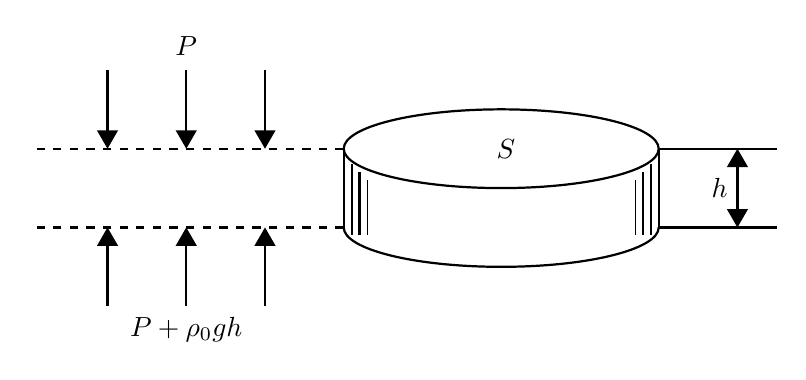
\begin{tikzpicture} [>=triangle 60,scale=1]
\draw [thick](0,0) ellipse (2cm and 0.5cm);
\path [fill=white,](-2,0) rectangle (2,1);
\draw [fill=white,thick](0,1) ellipse (2cm and 0.5cm);
\draw [thick](-2,0) -- (-2,1);
\draw [thick](2,0) -- (2,1);
\draw [thick](1.9,-.1) -- (1.9,0.8);
\draw [thick](1.8,-.1) -- (1.8,0.7);
\draw (1.7,-.1) -- (1.7,0.6);
\draw [thick](-1.9,-.1) -- (-1.9,0.8);
\draw [thick](-1.8,-.1) -- (-1.8,0.7);
\draw (-1.7,-.1) -- (-1.7,0.6);
\draw [thick, dashed](-2,1) -- (-6,1);
\draw [thick, dashed](-2,0) -- (-6,0);
\draw [thick](2,0) -- (3.5,0);
\draw [thick](2,1) -- (3.5,1);
\draw [thick,<->](3,1) -- (3,0);
\node [left] at (3,0.5) {$h$};
\node [left] at (0.3,1) {$S$};
\draw [thick,<-](-3,0) -- (-3,-1);
\draw [thick,<-](-4,0) -- (-4,-1);
\draw [thick,<-](-5,0) -- (-5,-1);
\draw [thick,<-](-3,1) -- (-3,2);
\draw [thick,<-](-4,1) -- (-4,2);
\draw [thick,<-](-5,1) -- (-5,2);
\node at (-4,2.3) {$P$};
\node at (-4,-1.3) {$P+\rho_{0}gh$};
\end{tikzpicture}
%\includegraphics[width=0.8\linewidth]{fig-066a.pdf}
\caption{Illustration for buoyant force for Archimedes' principle.}
\label{fig-67}
\end{figure}
Archimedes' principle can be deduced in a somewhat different way. Assume that the body immersed in the liquid has the form of a cylinder of height $h$ and that the area of its base is $S$ (\emph{Figure \ref{fig-67}}). Assume that the pressure on the upper base is $p$.

Then the pressure on the lower base will equal $p+\rho gh$. Thus, the difference in pressure on the upper and lower bases equals $\rho_{0}gh$. If we multiply this difference by the area $S$ of the base, we obtain the force $F=\rho ghS$ which tends to push the body upward. Since $hS=V$, the volume of the cylinder, it can readily be seen that this is the buoyant force which appears in Archimedes' principle.
\\
\textsc{Student A:} Yes, now I see that Archimedes' principle can be arrived at by purely logical reasoning.
\\
\textsc{Teacher:} Before proceeding any further, let us recall the condition for the floating of a body.
\\
\textsc{Student A:} I remember that condition. The weight of the body should be counterbalanced by the buoyant force acting on the body in accordance with Archimedes' principle.
\\
\textsc{Teacher:} Quite correct. Here is an example for you. A piece of ice floats in a vessel with water. Will the water level change when the ice melts?
\\
\textsc{Student A:} The level will remain unchanged because the weight of the ice is counterbalanced by the buoyant force and is therefore equal to the weight of the water displaced by the ice. When the ice melts it converts into water whose volume is equal to that of the water that was displaced previously.
\\
\textsc{Teacher:} Exactly. And now let us assume that there is, for instance, a piece of lead inside the ice. What will happen to the water level after the ice melts in this case?
\\
\textsc{Student A:} I'm not quite sure, but I think the water level should reduce slightly. I cannot, however, prove this.
\\
\textsc{Teacher:} Let us denote the volume of the piece of ice together with the lead by $V$, the volume of the piece of lead by $v$, the volume of the water displaced by the submerged part of the ice by $V_{1}$ the density of the water by $\rho_{0}$, the density of the ice by $\rho_{1}$ and the density of the lead by $\rho_{2}$. The piece of ice together with the lead has a weight equal to\\ 
\begin{equation*}%
\rho_{1} g (V-v) + \rho_{2}gv
\end{equation*}
This weight is counterbalanced by the buoyant force $\rho_{0}gV t$. Thus
\\
\begin{equation}%
\rho_{1} g (V-v) + \rho_{2}g v = \rho_{0}g V t
\label{eq-90}
\end{equation}
After melting, the ice turns into water whose volume $V_{2}$ is found from the equation\\
\begin{equation*}
\rho_{1} g (V-v) = \rho_{0} gV_{2}
\end{equation*}
Substituting this equation into (\ref{eq-90}) we obtain
\begin{equation*}%
\rho_{0}gV_{2} + \rho_{2}gv = \rho_{0}gV_{1}
\end{equation*}
From which we find that the volume of water obtained as a result of the melting of the ice is
\begin{equation}%
V_{2} = V_{1} -v \frac{\rho_{2}}{\rho_{1}}
\label{eq-91}
\end{equation}
Thus, before the ice melted, the volume of water displaced was $V_{1}$. Then the lead and the water from the melted ice began to occupy the volume $(V_{2}+v)$. To answer the question concerning the water level in the vessel, these volumes should be compared. From equation (\ref{eq-91}) we get
\\
\begin{equation}%
V_{2} + v= V_{1} - v \frac{\rho_{2}-\rho_{0}}{\rho_{0}}
\label{eq-92}
\end{equation}


Since $\rho_{2} > \rho_{0}$ (lead is heavier than water), it can be seen from equation (\ref{eq-92}) that $(V_{2}+v)<V_{1}$ Consequently, the water level will reduce as a result of the melting of the ice. Dividing the difference in the volumes $V_{1} - (V_{2}+v)$ by the cross-sectional area $S$ of the vessel (assuming, for the sake of simplicity, that it is of cylindrical shape) we can find the height $h$ by which the level drops after the ice melts. Thus
\begin{equation}
h= v \left( \frac{\rho_{2}-\rho_{0}}{\rho_{0}S} \right)
\label{eq-93}
\end{equation}

Do you understand the solution of this problem?
\\
\textsc{Student A:} Yes, I'm quite sure I do.
\\
\textsc{Teacher:} Then, instead of the piece of lead, let us put a piece of cork of volume $v$ and density $\rho_{3}$ inside the ice. What will happen to the water level when the ice melts?
\\
\textsc{Student A:} I think it will rise slightly.
\\
\textsc{Teacher:} Why?
\\
\textsc{Student A:} In the example with lead the level fell. Lead is heavier than water, and cork is lighter than water. Consequently, in the case of cork we should expect the opposite effect: the water level should rise.
\\
\textsc{Teacher:} You are mistaken. Your answer would be correct if the cork remained submerged after the ice melted. Since the cork is lighter than water it will surely rise to the surface and float. Therefore, the example with cork (or any other body lighter than water) requires special consideration. Using the
result of equation (\ref{eq-91}), we can find the difference between the volume of the water displaced by the piece of ice together with the cork, and that of the water obtained by the melting of the ice. Thus
\begin{equation}%
V_{1} - V_{2} = v \left( \frac{\rho_{3}}{\rho_{0}} \right)
label{eq-94}
\end{equation}

Next we apply the condition for the floating of the piece of cork:
\begin{equation}%
\rho_{3}v  = \rho_{0}v_{1}
label{eq-95}
\end{equation}
where $v_{1}$ is the volume of the part of the cork submerged in water. Substituting this equation into (\ref{eq-94}), we obtain
\begin{equation}%
V_{1} = V_{2} +v_{1}
label{eq-94}
\end{equation}

Thus the volume of water displaced by the piece of ice is exactly equal to the sum of the volume of water obtained from the melted ice. and the volume displaced by the submerged portion of the floating piece of cork. So in this case the water level remains unchanged.
\\
\textsc{Student A:} And if the piece of ice contained simply a bubble of air instead of the piece of cork?
\\
\textsc{Teacher:} After the ice melts, this bubble will be released. It can readily be seen that the water level in the' vessel will be exactly the same as it was before the ice melted. In short, the example with the bubble of air in the ice is similar to that with the piece of cork.
\\
\textsc{Student A:} I see that quite interesting questions and problems can be devised on the basis of Archimedes' principle.
\\
\textsc{Teacher:} Unfortunately, some examinees don't give enough attention to this principle when preparing for their physics examinations. Let us consider the following example. One pan of a balance
carries a vessel with water and the other, a stand with a weight suspended from it. The pans are balanced (\emph{Figure \ref{fig-68}(a)}). Then the stand is turned so that the suspended weight is completely submerged in the water. Obviously, the state of equilibrium is disturbed since the pan with the stand becomes lighter (\emph{Figure \ref{fig-68}(b)}). What additional weight must be put on the pan with the stand to restore equilibrium?

\begin{marginfigure}
\centering
\includegraphics[width=\linewidth,angle=-2]{fig-068a}
\caption{What additional weight must be put on the pan with the stand to restore equilibrium?}
\label{fig-68}
\end{marginfigure}

\textsc{Student A:} The submerged weight is subject to a buoyant force equal to the weight of the water of the volume displaced by the submerged weight (we denote this weight of water by $P$). Consequently, to restore equilibrium, a weight $P$ should be placed on the pan with the stand.
\\
\textsc{Teacher:} You are mistaken. You would do well to recall Newton's third law of motion. According to this law, the force with which the water in the vessel acts on the submerged weight is exactly equal to the force with which the submerged weight acts on the water in the opposite direction. Consequently, as the weight of the pan with the stand reduces, the weight of the pap with the vessel increases. Therefore, to restore equilibrium, a weight equal to $2P$ should be added to the pan with the stand.
\\
\textsc{Student A:} I can't quite understand your reasoning. After all, the interaction of the submerged weight and the water in no way resembles the interaction of two bodies in mechanics.
\\
Fig. 68
\textsc{Teacher:} The field of application of Newton's third law is not limited to mechanics. The expression ``to every action there is an equal and opposite reaction'' refers to a great many kinds
of interaction. We can, however, apply a different line of reasoning in our case, one to which you will surely have no objections. Let us deal with the stand with the weight and the vessel with the water as part of a single system whose total weight is obviously the sum of the weight of the left pan and that of the right pan. The total weight of the system should not change due to interaction of its parts with one another. Hence, if as the result of interaction the weight of the right pan is decreased by $P$, the weight of the left pan must be increased by the same amount ($P$). Therefore, after the weight is submerged in the vessel with water, the difference between the weights of the left and right pans should be $2P$.

\subsection{PROBLEM}
\begin{enumerate}[resume=problems]
\item A vessel of cylindrical shape with a cross-sectional area $S$ is filled with water in which a piece of ice, containing a lead ball, floats. The volume of the ice together with the lead ball is $V$ and $\dfrac{1}{20}$ of this volume is above the water level. To what mark will the water level in the vessel reduce after the ice melts? The densities of water, ice and lead are assumed to be known.
\end{enumerate}

\chapter{Is Archimedes' Principle Valid In A Spaceship?}
\label{ch-17}

\paragraph{}

\textsc{Teacher:} Is Archimedes' principle valid in a spaceship when it is in a state of weightlessness?
\\
\textsc{Student A:} I think it is not. The essence of Archimedes' principle is that due to the different
densities of. the body and the liquid (of equal volumes, of course), different amounts of work
are required to raise them to the same height. In a state of weightlessness, there is no difference in
these amounts of work since the work required to lift a body and that required to lift an equal
volume of the liquid is equal to zero.

We can reach the same conclusion if we consider the pressure of the liquid on a body submerged in it because the buoyant force is due to the difference in the pressures exerted on the bottom and top bases on the body. In a state of weightlessness, this difference in pressure vanishes and, with it, the buoyant force. I may add that in a state of weightlessness there is no difference between ``up'' and ``down'' and so it is impossible to indicate which base of the body is the upper and which the lower one.
Thus,' in a state of weightlessness, no buoyant force acts on a body submerged in a liquid. This means that Archimedes' principle is not valid for such a state.
\\
\textsc{Student B:} I don't agree with the final conclusion of Student A. I am sure that Archimedes' principle is valid for a state of weightlessness. Let us reason more carefully. We shall not pass over directly to a state of weightlessness, but begin with a lift travelling with a certain acceleration
a which is in the same direction as the acceleration g of gravity. Assume that $a < g$. It is easy to see that in the given case a body submerged in a liquid will be subject to the buoyant force

\begin{equation}%
F= \rho_{0} (g-a)V
\label{eq-96}
\end{equation}

and the weight of the liquid of a volume displaced by the body is also equal to $\rho_{0} (g-a)V$. Thus, the buoyant force is still equal to the weight of the liquid displaced by the body, i. e. Archimedes' principle is valid. Next we will gradually increase the acceleration $a$, approaching the value of $g$. According to equation (\ref{eq-96}), the buoyant force will be gradually reduced, but simultaneously and in exactly the same way, the weight of a volume of liquid equal to the volume of the body will also be reduced. In other words, as acceleration $a$ approaches acceleration $g$, Archimedes' principle will continue to be valid. In the limit $a=g$ a state of weightlessness sets in. At this the buoyant force becomes zero, but so does the weight of the liquid displaced by the body. Consequently, nothing prevents us from stating that Archimedes' principle is valid for a state of weightlessness as well. I wish to illustrate my argument by the following example. Let us suppose that a piece of cork floats in a vessel with water. According to equation (\ref{eq-95}) the ratio of the volume of the piece of cork submerged in the water to the total volume of the piece is equal to the ratio of the density of cork to the density of water. Thus
\begin{equation}%
\frac{v_{1}}{v} = \frac{\rho_{3}}{\rho_{0}}
\label{eq-97}
\end{equation}

Next, we suppose that this vessel is in a lift and the lift begins to descend with a certain acceleration $a$. Since this does not change the densities of cork and water, equation (\ref{eq-97}) holds. In other words, in the motion of the lift with acceleration, the position of the piece of cork with reference to the water level remains the same as in the absence of acceleration. Obviously, this condition will not change in the limiting case when $a=g$ and we reach a state of weightlessness. In this way, the position of the piece of cork with respect to the water level, determined by Archimedes' principle, turns out to be independent of the acceleration of the lift. In this case no distinction can be made between the presence and absence of weightlessness.
\\
\textsc{Teacher:} I should say that both of your arguments are well substantiated. However, I must agree with Student A: Archimedes' principle is not valid for a state of weightlessness.
\\
\textsc{Student B:} But then you must refute my proofs. 
\\
\textsc{Teacher:}That's just what I'll try to do. Your arguments are based on two main points. The first is that at an acceleration $a<g$ a body is buoyed up in the liquid in a manner fully complying with Archimedes' principle. The second is that this statement must hold for the limiting case as well, when $a=g$, i. e. a state of weightlessness is reached. I have no objection to the first point, but I don't agree with the second.
\\
\textsc{Student B:} But you can't deny that the piece of cork remains in the same position in a state of weightlessness as well t And its position directly follows from Archimedes' principle.
\\
\textsc{Teacher:} Yes, that's true. The piece of cork actually does remain in the same position in a state of weightlessness as well. However, in this state its position with respect to the surface of the liquid is no longer a result of Archimedes' principle. Push it deep into the water with your finger and it will remain suspended at the depth you left it. On the other hand, if there is even the smallest difference $(g-a)$ ,
the piece of cork will come up to the surface and float in the position determined by Archimedes' principle. Thus, there is a basic difference between weightlessness and the presence of even an insignificant weightness. In other words, in passing over to a state of weightlessness, at the ``very last instant'' there occurs an abrupt change, or jump, that alters the whole situation qualitatively.
\\
\textsc{Student B:} But what is this jump due to? Where did it come from? In my reasoning, acceleration a smoothly approached acceleration $g$.
\\
\textsc{Teacher:} This jump is related to the fact that at $a=g$, a certain symmetry appears: the difference between ``up'' and ``down'' disappears, which, incidentally, was very aptly pointed out by Student A. If the difference $(g-a)$ is infinitely small, but still not equal to zero, the problem contains a physically defined direction ``upward''. It is precisely in this direction that the buoyant force acts. However, at $a=g$, this direction disappears, and all directions become physically equivalent. That's what I mean by a jump. The destruction or the appearance of symmetry always occurs with jump.



\cleardoublepage
\thispagestyle{empty}
\vspace*{2cm}

\begin{figure*}
\centering
\includegraphics[width=0.65\linewidth]{sec-h.pdf}
%\caption{Velocity \emph{vs} time graph for the function shown in Figure \ref{fig-05}.}
%\label{fig-06}
\end{figure*}
%\addtocounter{figure}{1}
% For incrementing the figure numbers for figures without caption or numbering
\begin{fullwidth}
\begin{Large}
Basically, modern physics is molecular physics. Hence it is especially important to obtain some knowledge of the fundamentals of the molecular-kinetic theory of matter, if only by using the simplest example of the ideal gas. The question of the peculiarity in the thermal expansion of water is discussed separately. The gas laws will be analysed in detail and will be applied in the solution of specific engineering problems.
\end{Large}
\end{fullwidth}


\chapter{What Do You Know About The Molecular-Kinetic Theory Of Matter?}
\label{ch-18}
\paragraph{}
\textsc{Teacher:} One of the common examination questions is: what are the basic principles of the
molecular-kinetic theory of matter? How would you answer this question?
\\
\textsc{Student A:} I would mention the two basic principles. The first is that all bodies consist of molecules, and the second, that the molecules are in a state of chaotic thermal motion.
\\
\textsc{Teacher:} Your answer is very typical: laconic and quite incomplete. I have noticed that students usually take a formal attitude with respect to this question. As a rule, they do not know what should be said about the basic principles of the molecular-kinetic theory, and explain it away with just a few general remarks. In this connection, I feel that the molecular-kinetic theory of matter should be discussed in more detail. I shall begin by mentioning the principles of this theory that can be regarded as the basic ones.
\begin{enumerate}[label=\arabic*.,leftmargin=1cm]
\item Matter has a ``granular'' structure: it consists of molecules `(or atoms). One gram-molecule of a substance contains $N_{A} = \num{6d23}$ molecules regardless of the physical state of the substance (the number $N_{A}$ is called Avogadro's number).
\item The molecules of a substance are in a state of incessant thermal motion.
\item The nature of the thermal motion of the molecules depends upon the nature of their interaction and changes when the substance goes over from one physical state to another.
\item The intensity of the thermal motion of the molecules depends upon the degree to which the body is heated, this being characterized by the absolute temperature $T$. The theory proves that the mean energy $e$ of a separate molecule is proportional to the temperature $T$. Thus, for instance, for monoatomic (single-atom) moleculese
\begin{equation}
e = \frac{2}{3} kT 
\label{eq-98}
\end{equation}
where $k= \num{1.38d-16} \frac{\mathrm{erg}}{\mathrm{deg}}$ is a physical constant called Boltzmann's constant.

\item From the standpoint of the molecular-kinetic theory, the total energy $E$ of a body is the sum of the following terms: $E = E_{k} + E_{p} + U$ where $E_{k}$ is the kinetic energy of the body as a whole, $E_{p}$ is the potential energy of the body as a whole in a certain external field, and $U$ is the energy associated with the thermal motion of the molecules of the body. Energy $U$ is called the internal energy of the body. Inclusion of the internal energy in dealing with various energy balances is a characteristic feature of the molecular-kinetic theory.
\end{enumerate}
\textsc{Student B:} We are used to thinking that the gram-molecule and Avogadro's number refer to chemistry.
\\
\textsc{Teacher:} Evidently, that is why students taking a physics examination do not frequently know what a gram-molecule is, and, as a rule, are always sure that Avogadro's number refers only to gases. Remember: a gram-molecule is the number of grams of a substance which is numerically equal to its molecular weight (and by no means the weight of the molecule expressed in grams, as some students say); the gram-atom is the number of grams of a substance numerically equal to its atomic weight; and Avogadro's number is the number of molecules in a gram-molecule (or atoms in a gram-atom) of any substance, regardless of its physical state.

I want to point out that Avogadro's number is a kind of a bridge between the macro and micro characteristics of a substance. Thus, for example, using Avogadro's number, you can express such a micro characteristic of a substance as the mean distance between its molecules (or atoms) in terms of the density and molecular (or atomic) weight. For instance, let us consider solid iron. Its density is 
$\rho=\SI{7.8}{\gram\per\cubic\centi\metre}$ and atomic weight $A =56$. We are to find the mean distance between the atoms in iron. We shall proceed as follows: in $A\,\, \si{\gram}$ of iron there are $N_A$ atoms, then in \SI{1}{\gram} of iron there must be $\dfrac{N_{A}}{A}$ atoms. It follows that in \SI{1}{\cubic\centi\meter} there are $\rho \left( \dfrac{N_{A}}{A} \right)$ atoms. Thus each atom of iron is associated with a volume of  $\left( \dfrac{A}{\rho N_{A}} \right) \si{\cubic\centi\meter}$. The required mean distance between the atoms is approximately equal to the cube root of this volume\\
\begin{equation*}
x \approx \sqrt[3]{\frac{A}{\rho N_{A}}} =\sqrt[3]{\frac{56}{7.8\times \num{6d23}}} \,\, \si{\centi\meter} \approx \num{2d-8}\,\, \si{\centi\meter}
\end{equation*}
\textsc{Student B:} Just before this you said that the nature of the thermal motion of the molecules depends upon the intermolecular interaction and is changed in passing over from one physical state to another. Explain this in more detail, please.
%\begin{marginfigure}%
%\centering
%\includegraphics[width=\linewidth]{fig-069a}
%\caption{What additional weight must be put on the pan with the stand to restore equilibrium?}
%\label{fig-69}
%\end{marginfigure}


\begin{figure}
\centering
%\fbox{
\begin{tikzpicture}[>=triangle 45,scale=1.3]
\clip (-1,-1.6) rectangle (5, 4.8);
\draw[thick, ->,gray] (0,0) -- (5,0);
\draw[thick, ->,gray] (0,-1.8) -- (0,4.5);
\draw[thick, dashed,gray] (0,-1) -- (4,-1);
\node [left] at (0,4.5) {$E_{p}$};
\node [left] at (0,-1) {$e_{1}$};
\node [below left] at (4.8,0) {$r$};
\node [left] at (0,0) {0};
\draw[ultra thick,red] (0.1,3.4) .. controls (.38,-4.8) and (2.,0.).. (4.4, -0.1);
\draw[<-] (.7,0) -- (.7,-1);
\node [above] at (0.7,0) {$A$};
\draw[<-] (2.3,0) -- (2.3,-1);
\node [above] at (2.3,0) {$B$};
%\draw[gray,step=0.25] (-0.6,-3) grid (5, 5.3);
\end{tikzpicture}%}
\caption{Dependence of the potential energy $E_{p}$ of interaction of the molecules on the distance $r$ between their centres.}
\label{fig-69}
\end{figure}

\textsc{Teacher:} Qualitatively, the interaction of two molecules can be described by means of the curve illustrated in \emph{Figure \ref{fig-69}}. This curve shows the dependence of the potential energy $E_{p}$ of interaction of the molecules on the distance $r$ between their centres. At a sufficiently large distance between the molecules the curve $E_{p}(r)$ asymptotically approaches zero, i. e. the molecules practically cease to interact. As the molecules come closer together, the curve $E_{p}(r)$ turns downward. Then, when they are sufficiently close to one another, the molecules begin to repulse one another and curve $E_{p}(r)$ turns upward and $E$ continues to rise (this repulsion means that the molecules cannot freely penetrate into each other). As can be seen, the $E_{p}(r)$ curve has a characteristic minimum.
\\
\textsc{Student B:} What is negative energy?
\\
\textsc{Teacher:} As we know, energy can be measured from any value. For instance, we can measure the potential energy of a stone from ground level of the given locality, or we can measure it from sea level, it makes no difference. In the given case, the zero point corresponds to the energy of interaction between molecules separated from each other at an infinitely large distance. Therefore, the negative energy of the molecule means that it is in a bound state (bound with another molecule). To ``free'' this molecule, it is necessary to add some energy to it to increase the energy of the molecule to the zero level. Assume that the molecule has a negative energy $e_{1}$ (see \emph{Figure \ref{fig-69}}). It is evident from the curve that in this case the molecule cannot get farther away from its neighbour than point $B$ or get closer than point $A$. In other words, the molecule will vibrate between points $A$ and $B$ in the field of the neighbouring molecule (more precisely, there will be relative vibration of two molecules forming a bound system).

In a gas molecules are at such great distances from one another on an average that they can be regarded as practically noninteracting. Each molecule travels freely, with relatively rare collisions. Each molecule participates in three types of motion: translatory, rotary (the molecule rotates about its own axis) and vibratory (the atoms in the molecule vibrate with respect to one another). If a molecule is monoatomic it will have only translatory motion.

In a crystal the molecules are so close together that they form a single bound system. In this case, each molecule vibrates in some kind of general force field set up by the interaction of the whole collective of molecules. Typical of a crystal as a common bound system of molecules is the existence of an ordered three-dimensional structure - the crystal lattice. The lattice points are the equilibrium positions of the separate molecules. The molecules accomplish their complex vibratory motions about these positions. It should be noted that in some cases when molecules form a crystal, they continue to retain their individuality to some extent. In these cases, distinction is to be made between the vibration of the molecule in the field of the crystal and the vibration of the atoms in the separate molecules. This phenomenon occurs when the binding energy of the atoms in the molecules is substantially higher than the binding energy of the molecules themselves in the crystal lattice. In most cases, however, the molecules do not retain their individuality upon forming a crystal so that the crystal turns out to be made up, not of separate molecules, but of separate atoms. Here, evidently, there is no intramolecular vibration, but only the vibration of the atoms in the field of the crystal. This, then, is the minimum amount of information that examinees should possess about atomic and molecular thermal motions in matter. Usually, when speaking about the nature of thermal motions in matter, examinees get no farther than saying it is a ``chaotic motion'', thus trying to cover up the lack of more detailed knowledge of thermal motion.
\\
\textsc{Student B:} But you haven't said anything about the nature of the thermal motions of molecules in a liquid.
\\
\textsc{Teacher:} Thermal motions in a liquid are more involved than in other substances. A liquid occupying an intermediate position between gases and crystals exhibits, along with strong particle interaction, a considerable degree of disorder in its structure. The difficulty of dealing with crystals, owing to the strong interaction of the particles, is largely compensated for by the existence of an ordered structure-the crystal lattice. The difficulty of dealing with gases owing to the disordered position of the separate particles is compensated for by a practically complete absence of particle interaction. In the case of liquids, however, there are both kinds of difficulties mentioned above with no corresponding compensating factors. It can be said that in a liquid the molecules, as a rule, completely retain their individuality. A great diversity of motions exists in liquids: displacement of the molecules, their rotation, vibration of the atoms in the molecules and vibration of the molecules in the fields of neighbouring molecules. The worst thing is that all of these types of motion cannot, strictly speaking, be treated separately (or, as they say, in the pure form) because there is a strong mutual influence of the motions.
\\
\textsc{Student B:} I can't understand how translational motion of the molecule can be combined with its vibration in the fields of neighbouring molecules.
\\
\textsc{Teacher:} Various models have been devised in which attempts were made to combine these motions. In one model, for instance, it was assumed that the molecule behaves as follows: it vibrates for a certain length of time in the field set up by its neighbours, then it takes a jump, passing over into new surroundings, vibrates in these surroundings, takes another jump, etc. Such a model is called the ``jump-diffusion model''.
\\
\textsc{Student B:} It seems that is precisely the way in which atoms diffuse in crystals.
\\
\textsc{Teacher:} You are right. Only remember that in crystals this process is slower: jumps into a new environment occur considerably more rarely. There exists another model according to which a molecule in a liquid behaves as follows: it vibrates surrounded by its neighbours and the whole environment smoothly travels (``floats'') in space and is gradually deformed. This is called the ``continuous-diffusion model''.
\\
\textsc{Student B:} You said that a liquid occupies an intermediate position between crystals and gases. Which of them is it closer to?
\\
\textsc{Teacher:} What do you think?
\\
\textsc{Student B:} It seems to me that a liquid is closer to a gas.
\\
\textsc{Teacher:} In actuality, however, a liquid is most likely closer to a crystal. This is indicated by the similarity of their densities, specific heats and coefficients of volume expansion. It is also known that the heat of fusion is considerably less than the heat of vaporization. All these facts are evidence of the appreciable similarity between the forces of inter-particle bonding in crystals and in liquids. Another consequence of this similarity is the existence of elements of ordered arrangement in the atoms of a liquid. This phenomenon, known as ``short-range order'', was established in X-ray scattering experiments.
\\
\textsc{Student B:} What do you mean by short-range order?
\\
\textsc{Teacher:} Short-range order is the ordered arrangement of a certain number of the nearest neighbours about any arbitrarily chosen atom (or molecule). In contrast to a crystal, this ordered arrangement with respect to the chosen atom is disturbed as we move away' from it, and does not lead to the formation of a crystal lattice. At short distances, however, it is quite similar to the arrangement of the atoms of the given substance in the solid phase. Shown in \emph{Figure \ref{fig-70}(a)} is the long-range order for a chain of atoms. It can be compared with the short-range order
\emph{(a)} shown in \emph{Figure \ref{fig-70}(b)}.

\begin{figure}
\centering
%\fbox{
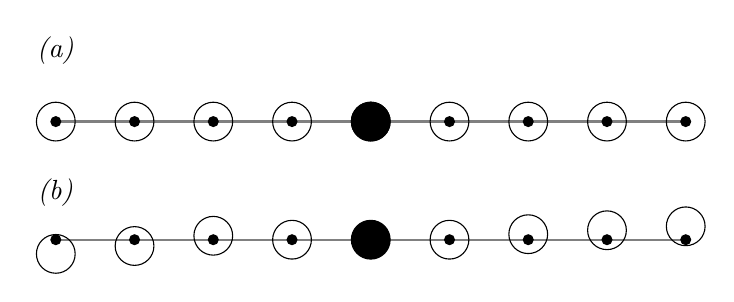
\begin{tikzpicture}
\draw[thick, gray] (0,0) -- (8,0);	
\foreach \x in {0,1,2,...,8}{
\draw (\x,0) circle (7pt);
\fill (\x,0) circle (2pt);}
\draw[fill] (4,0) circle (7pt);
\draw[thick, gray] (0,-1.5) -- (8,-1.5);	
\foreach \x in {0,1,2,...,8}{
\fill (\x,-1.5) circle (2pt);}
\draw (0,-1.68) circle (7pt);
\draw (1,-1.58) circle (7pt);
\draw (2,-1.45) circle (7pt);
\draw (3,-1.5) circle (7pt);
\draw[fill] (4,-1.5) circle (7pt);
\draw (5,-1.5) circle (7pt);
\draw (6,-1.43) circle (7pt);
\draw (7,-1.38) circle (7pt);
\draw (8,-1.33) circle (7pt);
\node [above] at (0,.6) {\emph{(a)}};
\node [above] at (0,-1.2) {\emph{(b)}};
\end{tikzpicture}%}
\caption{Long range order of crystals and short range order of liquids.}
\label{fig-70}
\end{figure}

The similarity between liquids and crystals has led to the term ``quasi-crystallinity'' of liquids.
\\
\textsc{Student B:} But in such a case, liquids can evidently be \emph{Figure \ref{fig-70}} dealt with by analogy with crystals.
\\
\textsc{Teacher:} I should warn you against misuse of the concept of quasi-crystallinity of liquids and attributing too much importance to it. Firstly, you must keep in mind that the liquid state corresponds to a wide range of temperatures, and the structural-dynamic properties of liquids cannot be expected to be the same (or even approximately the same) throughout this range. Near the critical state, a liquid should evidently lose all similarity to a solid and gradually transform to the gaseous phase. Thus, the concept of quasi-crystallinity of liquids may only be justified somewhere near the melting point, if at all. Secondly, the nature of the intermolecular interaction differs from one liquid to another. Consequently, the concept of quasi-crystallinity is not equally applicable to all liquids. For example, water is found to be a more quasi-crystalline liquid than molten metals, and this explains many of its special properties (see  Chapter \ref{ch-19}).
\\
\textsc{Student B:} I see now that there is no simple picture of the thermal motions of molecules in a liquid.
\\
\textsc{Teacher:} You are absolutely right. Only the extreme cases are comparatively simple. Intermediate cases are always complex.
\\
\textsc{Student A:} The physics entrance examination requirements include the question about the basis for the molecular-kinetic theory of matter. Evidently, one should talk about Brownian motion.
\\
\textsc{Teacher:} Yes, Brownian motion is striking experimental evidence substantiating the basic principles of the molecular-kinetic theory. But, do you know what Brownian motion actually is?
\\
\textsc{Student A:} It is thermal motion of molecules.
\\
\textsc{Teacher:} You are mistaken; Brownian motion can be observed with ordinary microscopes! It is motion of separate particles of matter bombarded by molecules of the medium in their thermal motion. From the molecular point of view these particles are macroscopic bodies. Nevertheless, by ordinary standards they are extremely small. As a result of their random uncompensated collisions with molecules, the Brownian particles move continuously in a haphazard fashion and thus move about in the medium, which is usually some kind of liquid.
\\
\textsc{Student B:} But why must the Brownian particles be so small? Why don't we observe Brownian motion with appreciable particles of matter such as tea leaves in a glass of tea?
\\
\begin{figure}
\centering
%\fbox{
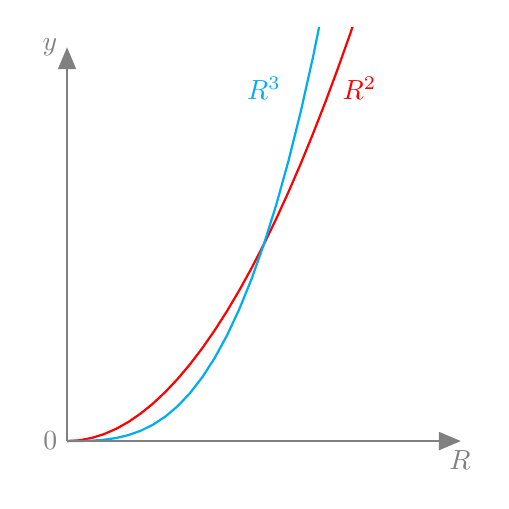
\begin{tikzpicture}[>=triangle 45,domain=0:1.5,scale=2.5]
	%\draw[gray,step=0.2] (-5,-5) grid (5, 5);
%	\clip (-1,-1) rectangle (3, 2.1);
	\clip (-0.2,-0.2) rectangle (2.1, 2.1);
	
	\draw[thick,red] plot (\x,\x*\x)	;
	\draw[thick,cyan] plot (\x,\x*\x*\x);
	\node[below right,red] at (1.35,1.9 ) {$R^{2}$};
	\node[below,cyan] at (1,1.9) {$R^{3}$};
		
	\draw[thick, ->, gray] (0,0) -- (2,0);
	\draw[thick, ->, gray] (0,0) -- (0,2);
	\node [left,gray] at (0,2) {$y$};
	\node [below left,gray] at (2.1,0) {$R$};
	\node [left,gray] at (0,0) {0};

\end{tikzpicture}%}
\caption{Effect of surface and volume relationships.}
\label{fig-71}
\end{figure}


\textsc{Teacher:} There are two reasons for this. In the first place, the number of collisions of molecules with the surface of a particle is proportional to the area of the surface; the mass of the particle is proportional to its volume. Thus, with an increase in the size $R$ of a particle, the number of colIisions of molecules with its surface increases proportionally to $\textcolor{red}{R^{2}}$, while the mass of the particle which is to be displaced by the collision increases in proportion to $\textcolor{cyan}{R^{3}}$. Therefore, as the particles increase in size it becomes more and more difficult for the molecules to push them about. To make this clear, I plotted two curves in \emph{Figure \ref{fig-71}}: $y=R^{2}$ and $y=R^{3}$. You can readily see that the quadratic relationship predominates at small values of $R$ and the cubic relationship at large values. This means that surface effects predominate at small values of $R$ and volume effects at large values.

In the second place, the Brownian particle must be very small since its collisions with molecules are uncompensated, i. e. the number of collisions from the left and from the right in unit time should differ substantially. But the ratio of this difference in the number of collisions to the whole number of collisions will be the greater, the less the surface of the particle.
\\
\textsc{Student A:} What other facts substantiating the molecular-kinetic theory are we expected to know?
\\
\textsc{Teacher:} The very best substantiation of the molecular- kinetic theory is its successful application in explaining a great number of physical phenomena. For example, we can give the explanation of the pressure of a gas on the walls of a vessel containing it. The pressure $p$ is the normal component of the force $F$ acting on unit area of the walls. Since
\begin{equation}
F=m \left( \frac{\Delta v}{\Delta t} \right) = \left( \frac{\Delta (mv)}{\Delta t} \right)
\label{eq-100}
\end{equation}
to find the pressure we must determine the momentum transmitted to a unit area of the wall surface per unit time due to the blows with which the molecules of the gas strike the walls. Assume that a molecule of mass $m$ is travelling perpendicular to a wall with a velocity $v$. As a result of an elastic collision with the wall, the molecule reverses its direction of travel and flies away from the wall with a velocity of $v$. The change in the momentum of the molecule equals $\Delta (mv)=m \Delta v=2mv$. This momentum is transmitted to the wall. For the sake of simplicity we shall assume that all the molecules of the gas have the same velocity $v$ and six directions of motion in both directions along three coordinate axes (assume that the wall is perpendicular to one of these axes). Next, we shall take into account that in unit time only those molecules will reach the wall which are at a distance within $v$ from it and whose velocity is directed toward the wall. Since a unit volume of the gas contains $\frac{N}{V}$ molecules. in unit time $\dfrac{1}{6}\left(\dfrac{N}{V} \right)v$ molecules strike a unit area of the wall surface. Since each of these molecules transmits a momentum of $2mv$, as a result of these blows a unit area of the wall surface receives a momentum equal to $2mv \dfrac{1}{6}\left(\dfrac{N}{V} \right)v$. According to equation (\ref{eq-100}). this is the required pressure $p$. Thus
\begin{equation}%
p= \frac{2}{3}\frac{N}{V} \frac{mv^{2}}{2}
\label{eq-101}
\end{equation}

According to equation (\ref{eq-98}), we can replace the energy of the molecule $\dfrac{mv^{2}}{2}$ by the quantity $\dfrac{3}{2} kT$ [in reference to the translational motion of molecules, equation (\ref{eq-98}) is valid for molecules with any number of atoms]. After this, equation (\ref{eq-101}) can be rewritten as
\begin{equation}%
pV=NkT
\label{eq-102}
\end{equation}
Note that this result was obtained by appreciable simplification of the problem (it was assumed, for instance, that the molecules of the gas travel with the same velocity). However, theory shows that this result completely coincides with that obtained in a rigorous treatment. Equation (\ref{eq-102}) is beautifully confirmed by direct measurements. It is good proof of the correctness of the concepts of the molecular-kinetic theory which were used for deriving equation (\ref{eq-102}).

Now let us discuss the phenomena of the evaporation and boiling of liquids on the basis of molecular-kinetic conceptions. How do you explain the phenomenon of evaporation?
\\
\textsc{Student A:} The fastest molecules of liquid overcome the attraction of the other molecules and fly out of the liquid.
\\
\textsc{Teacher:} What will intensify evaporation?
\\
\textsc{Student A:} Firstly, an increase in the free surface of the liquid, and secondly, heating of the liquid.
\\
\textsc{Teacher:} It should be remembered that evaporation is a two-way process: while part of the molecules leave the liquid, another part returns to it. Evaporation will be the more effective the greater the ratio of the outgoing molecules to the incoming ones. The heating of the liquid and an increase of its free surface intensify the escape of molecules from the liquid. At the same time, measures can be taken to reduce the return of molecules to the liquid. For example, if a wind blows across the surface of the liquid, the newly escaped molecules are carried away, thereby reducing the probability of their return. That is why wet clothes dry more rapidly in the wind. If the escape of molecules from a liquid and their return compensate each other, a state of dynamic equilibrium sets in, and the vapour above the liquid becomes saturated. In some cases it is useful to retard the evaporation process. For instance, rapid evaporation of the moisture in bread is undesirable. To prevent fast drying of bread it is kept in a closed container (bread box, plastic bag). This impedes the escape of the evaporated molecules, and a layer of saturated vapour is formed above the surface of the bread, preventing further evaporation of water from the bread.
\\
Now, please explain the boiling process.
\\
\textsc{Student A:} The boiling process is the same as evaporation, but proceeds more intensively.
\\
\textsc{Teacher:} I don't like your definition of the boiling process at all. I should mention that many examinees do not understand the essence of this process. When a liquid is heated, the solubility of the gases it contains reduces. As a result, bubbles of gas are formed in the liquid (on the bottom and walls of the vessel). Evaporation occurs in these bubbles, they become filled with saturated vapour, whose pressure increases with the temperature of the liquid. At a certain temperature, the pressure of the saturated vapour inside the bubbles becomes equal to the pressure exerted on the bubbles from the outside (this pressure is equal to the atmospheric pressure plus the pressure of the layer of water above the bubble). Beginning with this instant, the bubbles rise rapidly to the surface and the liquid boils. As you can see, the boiling of a liquid differs essentially from evaporation. Note that evaporation takes place at any temperature, while boiling occurs at a definite temperature called the boiling point. Let me remind you that if the boiling process has begun, the temperature of the liquid cannot be raised, no matter how long we continue to heat it. The temperature remains at the boiling point until all of the liquid has boiled away.
\\
It is evident from the above discussion that the boiling point of a liquid is depressed when the outside pressure reduces. In this. connection, let us consider the following problem. \emph{A flask contains a small amount of water at room temperature. We begin to pump out the air above the water from the flask with a vacuum pump. What will happen to the water?}
\\
\textsc{Student A:} As the air is depleted, the pressure in the flask will reduce and the boiling point will be depressed. When it comes down to room temperature, the water will begin to boil.
\\
\textsc{Teacher:} Could the water freeze instead of boiling?
\\
\textsc{Student A:} I don't know. I think it couldn't.
\\
\textsc{Teacher:} It all depends upon the rate at which the air is pumped out of the flask. If this process is sufficiently slow, the water should begin to boil sooner or later. But if the air is exhausted very rapidly, the water should, on the contrary, freeze. As a result of the depletion of the air (and, with it, of the water vapour), the evaporation process is' intensified. Since in evaporation the molecules with the higher energies escape from the water, the remaining water will be cooled. If the air is exhausted slowly, the cooling effect is compensated for by the transfer of heat from the outside. As a result the temperature of the water remains constant. If the air is exhausted very rapidly, the cooling of the water cannot be compensated by an influx of heat from the outside, and the temperature of the water begins to drop. As soon as this happens, the possibility of boiling is also reduced. Continued rapid exhaustion of the air from the flask will lower the temperature of the water to the freezing point, and the un-evaporated remainder of the water will be transformed into ice.



\chapter{How Do You Account For The Peculiarity In The Thermal Expansion Of Water?}
\label{ch-19}
\paragraph{}
\textsc{Teacher:} What are the peculiarities of the thermal expansion of water?
\\
\textsc{Student A:} When water is heated from \SIrange{0}{4}{\degreeCelsius} its density increases. It begins to expand only when its temperature is raised above \SI{4}{\degreeCelsius}.
\\
\textsc{Teacher:} How do you explain this?
\\
\textsc{Student A:} I don't know.
\\
\begin{marginfigure}
\centering
\includegraphics[width=\linewidth]{fig-072a}
\caption{Explaining peculiarity of thermal expansion of water.}
\label{fig-72}
\end{marginfigure}


\textsc{Teacher:} This distinctive feature of water is associated with its atomic structure. Molecules
of water can interact only in one way: each molecule of water can add on only four neighbouring
molecules whose centres then form a tetrahedron (\emph{Figure \ref{fig-72}}). This results in a friable, lace-like structure indicative of the quasi-crystallinity of water. Of course, we can speak of the structure of water, as of any other liquid, only on a short-range level (see  Chapter \ref{ch-18}). With an increase in the distance from
a selected molecule this order will undergo gradual distortion due to the bending and rupture of intermolecular bonds. As the temperature is raised, the bonds between the molecules are ruptured more frequently, there are more and more molecules with unoccupied bonds filling the vacancies of
the tetrahedral structure and, consequently, the degree of quasi-crystallinity is reduced. The above-mentioned lace-like structure of water as a quasi-crystalline substance convincingly explains the anomaly of the physical properties of water, in particular, the peculiarity of its thermal expansion. On one hand, an increase in temperature leads to an increase in the mean distances between the atoms
and molecule due to the intensification of intramolecular vibrations, i. e. the molecules seem to ``swell'' slightly. On the her hand, an increase in temperature breaks up the lace-like structure of water which, naturally, leads to a more dense packing of the molecules themselves. The first (vibrational) effect should lead to a reduction in the density of water. This is the common effect causing the thermal expansion of solids. The second effect, that of structure breakup, should, on the contrary, increase the density of water as it is heated. In heating water to \SI{4}{\degreeCelsius}, the structural effect predominates and the density of water consequently increases. Upon further heating, the vibrational effect begins to predominate and
therefore the density of water is reduced.

\chapter{How Well Do You Know The Gas Laws?}
\label{ch-20}

\paragraph{}
\indent
\textsc{Teacher:} Please write the equation for the combined gas law.
\\
\textsc{Student A:} This equation is of the form
\begin{equation}%
\frac{pV}{T} = \frac{p_{0}V_{0}}{T_{0}}
\label{eq-103}
\end{equation}

where $p$, $V$ and $T$ are the pressure, volume and temperature of a certain mass of gas in a certain
state, and $p_{0}$, $V_{0}$ and $T_{0}$ are the same for the initial state. The temperature is expressed in the absolute scale.
\\
\textsc{Student B:} I prefer to use an equation of a different form
\begin{equation}%
pV = \frac{m}{\mu} RT
\label{eq-104}
\end{equation}

where $m$ is the mass of the gas, $\mu$ is the mass of one gram-molecule and $R$ is the universal gas constant.
\\
\textsc{Teacher:} Both versions of the combined gas law are correct. (To Student B) You have used the universal gas constant. Tell me, how would you compute its value? I don't think one can memorize it.
\\
\textsc{Student B:} To compute $R$, I can use equation (\ref{eq-103}), in which the parameters $p$, $V_{0}$ and $T_{0}$ refer to a given mass of gas but taken at standard conditions. This means that $P_{0}= \SI{76}{\centi\meter}$ Hg (\si{\centi\meter} of mercury column), $T_{0}=\SI{273}{\kelvin}$ and $V_{0} =\left( \dfrac{m}{\mu} \right) \times \SI{22.4}{\litre}$, since a gram-molecule of any gas at standard conditions occupies a definite volume equal to \SI{22.4}{\litre}. The ratio $\frac{m}{\mu}$ is evidently the number of gram-molecules contained in the given mass of the gas. Substituting these values in equation (\ref{eq-103}) we obtain
\begin{equation*}%
pV = \left( \frac{m}{\mu}\right) \, T \,\, \left( \frac{\SI{76}{\centi\meter} \,\,\text{Hg} \times \SI{22.4}{\litre}}{\SI{273}{\kelvin}} \right)
\end{equation*}

Comparing this with expression (\ref{eq-104}) we find that $R=6.2 (\si{\centi\meter} \text{Hg}) \dfrac{\text{litres}}{\text{deg}}$.
\\
\textsc{Teacher:} I purposely asked you to do these calculations in order to demonstrate the equivalence of expressions (\ref{eq-103}) and (\ref{eq-104}). Unfortunately, examinees usually know only equation (\ref{eq-103}) and are unfamiliar with (\ref{eq-104}), which coincides with equation (\ref{eq-102}) obtained previously on the basis of molecular-kinetic considerations. From a comparison of equations (\ref{eq-102}) and (\ref{eq-104}) it follows that $\left( \dfrac{m}{\mu} \right)R=Nk$. Then

\begin{equation}
R=\frac{N}{\left( \dfrac{m}{\mu} \right)} k =N_{A}k
\label{eq-105}
\end{equation}
Thus the universal gas constant turns out to be the product of Avogadro's number by Boltzmann's constant. Next, we shall see whether you can use the equation of the combined gas law. Please draw a curve showing an isobaric process, i. e. a process in which the gas pressure remains constant, using coordinate axes $V$ and $T$.
\\
\textsc{Student A:} I seem to recall that this process is described by a straight line.
\\
\textsc{Teacher:} Why recall? Make use of equation (\ref{eq-104}). On its basis, express the volume of the gas as a function of its temperature.
\\
\textsc{Student A:} From equation (\ref{eq-104}) we get
\begin{equation}%
V = \left( \dfrac{m}{\mu} \right) \left( \dfrac{R}{p} \right) T
\label{106}
\end{equation}
\textsc{Teacher:} Does the pressure here depend upon the temperature?
\\
\textsc{Student A:} In the given case it doesn't `because we are dealing with an isobaric process.
\\
\textsc{Teacher:} Good. Then the product $\left( \dfrac{m}{\mu} \right) \left( \dfrac{R}{p} \right)$ in equation (\ref{eq-106}) is a constant factor. We thus obtain a linear dependence of the volume of the gas on its temperature. Examinees can usually depict \textcolor{red}{isobaric} ($p$=const), \textcolor{violet}{isothermal} ($T$=const) and \textcolor{cyan}{isochoric} ($V$=const) processes in diagrams with coordinate axes $p$ and $V$. At the same time they usually find it difficult to depict these processes with other sets of coordinate axes, for instance $V$ and $T$ or $T$ and $p$. These three processes are shown in \emph{Figure \ref{fig-73}} in different sets of coordinate axes.


\begin{figure*}
\centering
%\fbox{
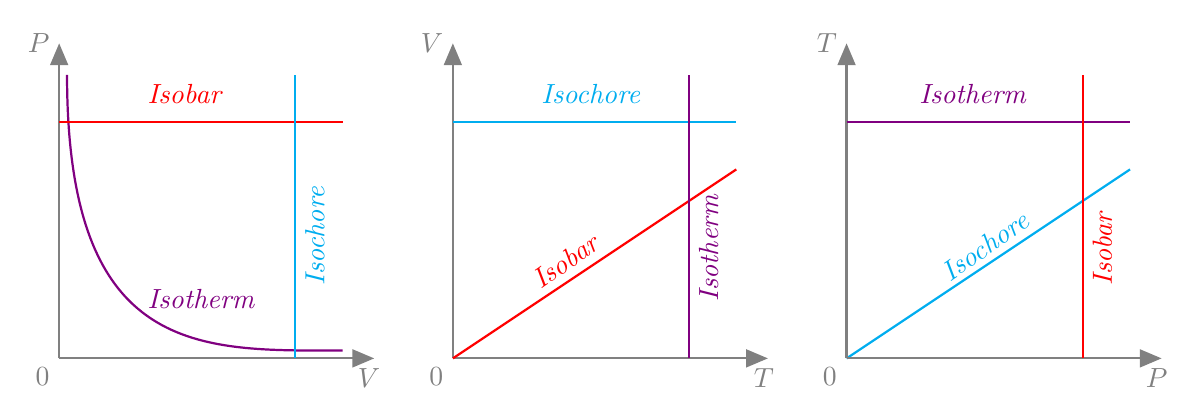
\begin{tikzpicture}
[>=triangle 45,scale=2]
	
	\clip (-2.7,-0.21) rectangle (4.55, 2.1);
	%\draw[gray,step=0.2] (-3,-1) grid (5, 3);
	
	\node[below right,red] at (-2,1.8 ) 
	{\emph{Isobar}};
	\node[below right,cyan] at (.5,1.8 ) 
	{\emph{Isochore}};
	\node[below right,violet] at (2.9,1.8 ) 
	{\emph{Isotherm}};
	
	\node[below right,cyan,rotate=90] at (-1,.4 ) 
	{\emph{Isochore}};
	\node[below right,violet,rotate=90] at (1.5,.3 ) 
	{\emph{Isotherm}};
	\node[below right,red,rotate=90] at (4,.4 ) 
	{\emph{Isobar}};

	\node[below right,violet,] at (-2,.5 ) 
	{\emph{Isotherm}};
	\node[below right,red,rotate=35] at (0.4,.55 ) 
	{\emph{Isobar}};
	\node[below right,cyan,rotate=35] at (3,.6 ) 
	{\emph{Isochore}};
		
	\draw[thick, ->, gray] (0,0) -- (2,0);
	\draw[thick, ->, gray] (0,0) -- (0,2);

	\node [left,gray] at (-2.5,2) {$P$};
	\node [left,gray] at (0,2) {$V$};
	\node [left,gray] at (2.5,2) {$T$};
	
	\node [below left, gray] at (2.1,0) {$T$};
	\node [below left, gray] at (4.6,0) {$P$};
	\node [below left, gray] at (-.4,0) {$V$};
	
	\node [below left,gray] at (0,0) {0};
	\node [below left,gray] at (2.5,0) {0};
	\node [below left,gray] at (-2.5,0) {0};
	
	\draw[thick, violet] (-2.45,1.8) .. controls (-2.45,0) and (-1.6,.05) .. (-.7,.05);
	\draw[thick, cyan] (2.5,0) -- (4.3,1.2);
	\draw[thick, red] (0,0) -- (1.8,1.2);


	
	\draw[thick, ->, gray] (2.5,0) -- (4.5,0);
	\draw[thick, ->, gray] (2.5,0) -- (2.5,2);
	
	\draw[thick, ->, gray] (-2.5,0) -- (-.5,0);
	\draw[thick, ->, gray] (-2.5,0) -- (-2.5,2);
	
	\draw[thick, red] (-2.5,1.5) -- (-.7,1.5);
	\draw[thick, cyan] (0,1.5) -- (1.8,1.5);
	\draw[thick, violet] (2.5,1.5) -- (4.3,1.5);
	
	\draw[thick, cyan] (-1,0) -- (-1,1.8);
	\draw[thick, violet] (1.5,0) -- (1.5,1.8);
	\draw[thick, red] (4,0) -- (4,1.8);
\end{tikzpicture}%}
\caption{The Gas Laws.}
\label{fig-73}
\end{figure*}

\textsc{Student B:} I have a question concerning isobars in a diagram with coordinate axes $V$ and $T$. From equation (\ref{eq-106}) and from the corresponding curve in \emph{Figure \ref{fig-73}} we see that as the temperature approaches zero, the volume of the gas also approaches zero. However, in no case can the volume of a gas become less than the total volume of all its molecules. Where is the error in my reasoning?
\\
\textsc{Teacher:} Equations (\ref{eq-102}), (\ref{eq-103}), (\ref{eq-104}) and (\ref{eq-106}) refer to the so-called ideal gas. The ideal gas is a simplified model of a real gas in which neither the size of the molecules nor their mutual attraction is taken into consideration. All the curves in \emph{Figure \ref{fig-73}} apply to such a simplified model, i. e. the ideal gas.
\\

\textsc{Student B:} But the gas laws agree well with experimental data, and in experiments we deal with real gases whose molecules have sizes of their own.
\\
\textsc{Teacher:} Note that such experiments are never conducted at extremely low temperatures. If a real gas has not been excessively cooled or compressed, it can be described quite accurately by the ideal gas model. Note also that for the gases contained in the air (for instance, nitrogen and oxygen), these conditions are met at room temperatures and ordinary pressures.
\\
\textsc{Student B:} Do you mean that if we plot the dependence of the volume on the temperature in an isobaric process for a real gas, the curve will coincide with the corresponding straight line in \emph{Figure \ref{fig-73}} at sufficiently high temperatures but will not coincide in the low temperature zone?
\\
\textsc{Teacher:} Exactly. Moreover, remember that on a sufficiently large drop in temperature a gas will be condensed into a liquid.
\\
\textsc{Student B:} I see. The fact that the curve of equation (\ref{eq-106}) in \emph{Figure \ref{fig-73}}  passes through the origin, or zero point, has no physical meaning. But then maybe we should terminate the curve before it reaches this point?
\\
\textsc{Teacher:} That is not necessary. You are just drawing the curves for the model of a gas. Where this model can be applied is another question. Now I want to propose the following. Two isobars are shown in \emph{Figure \ref{fig-74}}  in coordinate axes $V$ and $T$: one corresponds to the pressure $p_{1}$ and the other to the pressure $p_{2}$. Which of these pressures is higher?
\\
\textsc{Student A:} Most likely, $p_{2}$ is higher than $p_{1}$.
\\
\begin{marginfigure}[-3cm]
\centering
%\fbox{
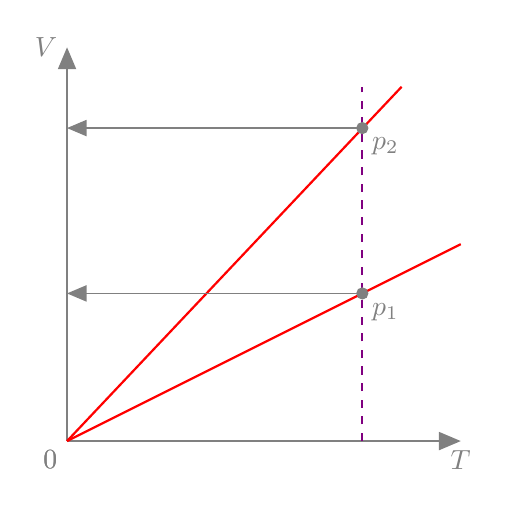
\begin{tikzpicture}	[>=triangle 45,scale=2.5]
	
	\clip (-.2,-0.21) rectangle (2.1, 2.1);
	%\draw[gray,step=0.2] (-3,-1) grid (5, 3);
		
	%\draw[thick,red] plot (\x,\x*\x)	;
	%\draw[thick,cyan] plot (\x,\x*\x*\x);
	
	%\node[below right,cyan] at (.5,1.8 ) 
	%{\emph{Isochore}};
	
	%\node[below right,violet,rotate=90] at (1.5,.3 ) 
	%{\emph{Isotherm}};
		
	\draw[thick, ->, gray] (0,0) -- (2,0);
	\draw[thick, ->, gray] (0,0) -- (0,2);
	\draw[thick, violet, dashed] (1.5,0) -- (1.5,1.8);

	\node [left,gray] at (0,2) {$V$};
	\node [below left, gray] at (2.1,0) {$T$};
	\node [below left,gray] at (0,0) {0};
	\node [below left,gray] at (0,0) {0};
	\node [below right,gray] at (1.5,.75) {$p_{1}$};
	\node [below right,gray] at (1.5,1.59) {$p_{2}$};
	
	\draw[thick, red] (0,0) -- (2,1);
	\draw[thick, red] (0,0) -- (1.7,1.8);
	\draw[<-,semithick,gray] (0,1.59) -- (1.5,1.59);
	\draw [fill,gray](1.5,1.59) circle (0.8pt);
	\draw[<-,semithick,gray] (0,.75) -- (1.5,.75);
	\draw [fill,gray](1.5,.75) circle (0.8pt);
\end{tikzpicture}%}
\caption{Which pressure is higher?}
\label{fig-74}
\end{marginfigure}

\textsc{Teacher:} You answer without thinking. Evidently, you decided that since that isobar is steeper, the corresponding pressure is higher. This, however, is entirely wrong. The tangent of the angle of inclination of an isobar equals  $\left( \dfrac{m}{\mu} \right) \left( \dfrac{R}{p} \right)$ according to equation (ref{eq-106}). It follows that the higher the pressure, the less the angle of inclination of the isobar. Thus, in our case, $p_{2} < p_{1}$ We can reach the same conclusion by different reasoning. Let us draw an isotherm in Fig. 74 (see the dashed line). It intersects isobar $p_{2}$ at a higher value of the gas volume than isobar $p_{1}$. We know that at the same temperature, the pressure of the gas will be the higher, the smaller its volume. This follows directly from the combined gas law [see equation (\ref{eq-103}) or (\ref{eq-104})]. Consequently,  $p_{2} < p_{1}$.
\\
\textsc{Student A:} Now, I'm sure I understand.
\\
\textsc{Teacher:} Then look at \emph{Figure \ref{fig-75}} which shows two isotherms (the coordinate axes are $p$ and $V$) plotted for the same mass of gas at different temperatures, $T_{1}$ and $T_{2}$ Which is the higher temperature?
\\
\begin{marginfigure}[-3cm]
\centering
%\fbox{
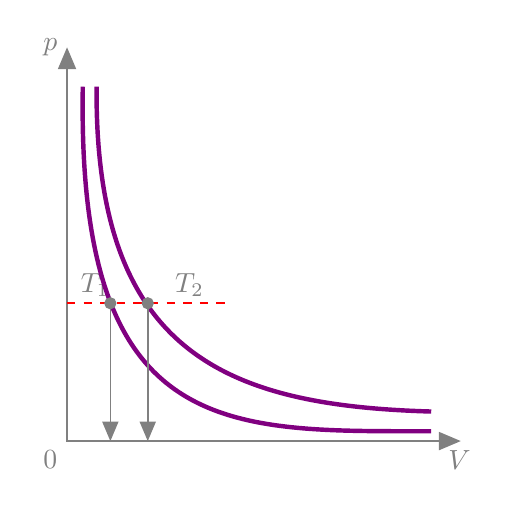
\begin{tikzpicture}[>=triangle 45,scale=2.5]
	
	\clip (-.2,-0.21) rectangle (2.1, 2.1);
%	\draw[gray,step=0.2] (-3,-1) grid (5, 3);
		
	%\draw[thick,red] plot (\x,\x*\x)	;
	%\draw[thick,cyan] plot (\x,\x*\x*\x);
	
	%\node[below right,cyan] at (.5,1.8 ) 
	%{\emph{Isochore}};
	
	%\node[below right,violet,rotate=90] at (1.5,.3 ) 
	%{\emph{Isotherm}};
		
	\draw[thick, <->, gray] (2,0) -- (0,0) -- (0,2);
	\draw[thick, red, dashed] (0,0.7) -- (.8,0.7);

	\node [left,gray] at (0,2) {$p$};
	\node [below left, gray] at (2.1,0) {$V$};
	\node [below left,gray] at (0,0) {0};
	\node [below right,gray] at (.02,.9) {$T_{1}$};
	\node [below right,gray] at (.5,.9) {$T_{2}$};
	
	
	%
	\draw[ultra thick, violet] (.08,1.8) .. controls (.05,.01) and (.8,.05) .. (1.85,.05);
	
\draw[ultra thick, violet] (.15,1.8) .. controls (.14,.45) and (.8,.18) .. (1.85,.15);
	
	\draw[->,semithick,gray] (0.22,.7) -- (0.22,0);
	\draw [fill,gray](0.22,.7) circle (0.8pt);
	\draw[->,semithick,gray] (0.41,.7) -- (0.41,0);
	\draw [fill,gray](0.41,.7) circle (0.8pt);

\end{tikzpicture}%}
\caption{Which pressure is higher?}
\label{fig-75}
\end{marginfigure}

\textsc{Student A:} First I shall draw an isobar (see the dashed line in \emph{Figure \ref{fig-75}}). At a constant pressure, the higher the temperature of a gas, the larger its volume. Therefore, the outermost isotherm $T_{2}$ corresponds to the higher temperature.
\\
\textsc{Teacher:} Correct. Remember: the closer an isotherm is to the origin of the coordinates $p$ and $V$, the lower the temperature is.
\\
\textsc{Student B:} In secondary school our study of the gas laws was of much narrower scope than our present discussion. The combined gas law was just barely mentioned. Our study was restricted to Boyle and Mariette's, Gay-Lussac's and Charles' laws.
\\
\textsc{Teacher:} In this connection, I wish to make some remarks that will enable the laws of Boyle and Mariotte, Gay-Lussac and Charles to be included in the general scheme. Boyle and Mariotte's law (more commonly known as Boyle's law) describes the dependence of $p$ on $V$ in an isothermal process. The equation for this law is of the form

\begin{equation}%
p=\frac{\text{constant}}{V}
\label{107}
\end{equation}

where the $\text{constant}= \left( \dfrac{m}{\mu} \right) RT$.

Gay-Lussac s law describes the dependence of $p$ on $T$ in an isochoric process. The equation of this law is
\begin{equation}%
p=\text{constant} \,\,T
\label{108}
\end{equation}
where the $\text{constant}= \left( \dfrac{m}{\mu} \right) \dfrac{R}{V}$.

The law of Charles describes the dependence of $V$ on $T$ in an isobaric process. Its equation is
\begin{equation}%
v=\text{constant} \,\,T
\label{109}
\end{equation}

where the $\text{constant}= \left( \dfrac{m}{\mu} \right) \dfrac{R}{p}$. [Equation (\ref{eq-109}) evidently repeats equation (\ref{eq-106}).] I will make the following remarks concerning the above-mentioned gas laws:

\begin{enumerate}
\item All these laws refer to the ideal gas and are applicable to a real gas only to the extent that the latter is described by the model of the ideal gas.
\item Each of these laws establishes a relationship between some pair of parameters of a gas under the assumption that the third parameter is constant.
\item As can readily be seen, each of these laws is a corollary of the combined gas law [see equation (\ref{eq-104})] which establishes a relationship between all three parameters regardless of any special conditions.
\item The constants in each of these laws can be expressed, not in terms of the mass of the gas and the constant third parameter, but in terms of the same pair of parameters taken for a different state of the same mass of the gas. In other words, the gas laws can be rewritten in the following form
\begin{align}
p & = \frac{p_{0}V_{0}}{V}
\tag{107a}
\label{107a}
\\
p & = \frac{p_{0}}{T_{0}} T
\tag{108a}
\label{108a}
\\
V & = \frac{V_{0}}{T_{0}} T
\tag{109a}
\label{109a}
\end{align}

\end{enumerate}
\textsc{Student A:} It seems I have finally understood the essence of the gas laws.
\\
\textsc{Teacher:} In that case, let us go on. Consider the following example. A gas expands in such a manner that its pressure and volume comply with the condition
\begin{equation}
pV^{2} = \text{constant}
\label{eq-110}
\end{equation}

We are to find out whether the gas is heated or, on the contrary, cooled in such an expansion.
\\
\textsc{Student A:} Why must the temperature of the gas change?
\\
\begin{marginfigure}
\centering
\includegraphics[width=\linewidth]{fig-076a}
\caption{Isochores for $p \propto \dfrac{1}{V^{2}}$.}
\label{fig-76}
\end{marginfigure}
\textsc{Teacher:} If the temperature remained constant, that would mean that the gas expands according to the law of Boyle and Mariotte [equation (\ref{eq-107})]. For an isothermal process $p \propto \dfrac{1}{V}$, while in our case the dependence of $p$ on $V$ is of a different nature: $p \propto \dfrac{1}{V^{2}}$).
\\
\textsc{Student A:} Maybe I can try to plot these relationships? The curves will be of the shape shown in \emph{Figure \ref{fig-76}}.
\\
\textsc{Teacher:} That's a good idea. What do the curves suggest?
\\
\textsc{Student A:} I seem to understand now. We can see that in tracing the curve $p \propto \dfrac{1}{V^{2}}$ toward greater volumes, the gas will gradually pass over to isotherms that are closer and closer to the origin, i.e, isotherms corresponding to ever-decreasing temperatures. This means that in this expansion process the gas is cooled.
\\
\textsc{Teacher:} Quite correct. Only I would reword your answer. It is better to say that such a gas expansion process is possible only provided the gas is cooled.
\\
\textsc{Student B:} Can we reach the same conclusion analytically?
\\
\textsc{Teacher:} Of course. Let us consider two states of the gas: $p_{1}, \,V_{1}, \,T_{1}$ and $p_{2},\, V_{2},\, T_{2}$. Next we shall write the combined gas law [see equation (\ref{eq-104})] for each of these states
\begin{align*}%
p_{1} V_{1} & = \frac{m}{\mu} RT_{1}\\
p_{2}V_{2} & = \frac{m}{\mu} RT_{2}
\end{align*}
We can write the given gas expansion process, according to the condition, in the form
\begin{equation*}%
p_{1} V_{1}^{2} = p_{2}V_{2}^{2}
\end{equation*}

Substituting the two preceding equations of the gas law in the last equation, we obtain
\begin{equation*}%
\frac{m}{\mu} R T_{1} V_{1} = \frac{m}{\mu} R T_{2}V_{2}
\end{equation*}
After cancelling the common factors we find that
\begin{equation}
T_{1} V_{1} = T_{2}V_{2}
\label{eq-111}
\end{equation}
From this equation it is evident that if the gas volume is, for example, doubled, its temperature (in the absolute scale) should be reduced by one half.
\\
\textsc{Student A:} Does this mean that whatever the process, the gas parameters ($p$, $V$ and $T$) will be related to one another in each instant by the combined gas law?
\\
\begin{marginfigure}
\centering
\includegraphics[width=\linewidth]{fig-077a}
\caption{Work done by a gas.}
\label{fig-77}
\end{marginfigure}
\textsc{Teacher:} Exactly. The combined gas law establishes a relationship between the gas parameters regardless of any conditions whatsoever. Now let us consider the nature of the energy exchange between a gas and its environment in various processes. Assume that the gas is expanding. It will move back all bodies restricting its volume (for instance, a piston in a cylinder). Consequently, the gas performs work on these bodies. This work is not difficult to calculate for isobaric expansion of the gas. Assume that the gas expands isobarically and pushes back a piston of cross-sectional area $S$ over a distance $\Delta l$ (\emph{Figure \ref{fig-77}}). The pressure exerted by the gas on the piston is $p$. Find the amount of work done by the gas in moving the piston: 
\begin{equation}%
A = F \Delta l = (pS) \Delta l = p (S \Delta l) = p(V_{2} - V_{1})
\end{equation}

where $V_{1}$ and $V_{2}$ are the initial and final volumes of the gas. The amount of work done by the gas in nonisobaric expansion is more difficult to calculate because the pressure varies in the course of gas expansion. In the general case, the work done by the gas when its volume increases from $V_{1}$ to $V_{2}$ is equal to the area under the $p (V)$ curve between the ordinates $V_{1}$ and $V_{2}$. The amounts of work done by a gas in isobaric and in isothermal expansion from volume V 1 to volume V 2 are shown in \emph{Figure \ref{fig-78}} by the whole hatched area and the crosshatched area, respectively. The initial state of the gas is the same in both cases. Thus, in expanding, a gas does work on the surrounding bodies at the expense of part of its internal energy. The work done by the gas depends upon the nature of the expansion process. Note also that if a gas is compressed, then work is done on the gas and, consequently, its internal energy increases.

\begin{marginfigure}%
\centering
\includegraphics[width=\linewidth]{fig-078a}
\caption{Work done by a gas.}
\label{fig-78}
\end{marginfigure}

The performance of work, however, is not the only method of energy exchange between a gas and the medium. For example, in isothermal expansion a gas does a certain amount of work $A$ and, therefore, loses an amount of energy equal to $A$. On the other hand, however, as follows from the principles enumerated in Chapter \ref{ch-18} [see equation (\ref{eq-98})], a constant temperature of the gas in an isothermal process should mean that its internal energy $U$ remains unchanged (let me remind you that $U$ is determined by the thermal motion of the molecules and that the mean energy of the molecules is proportional to the temperature $T$). The question is: what kind of energy is used to perform the work in the given case?
\\
\textsc{Student B:} Evidently, the heat transmitted to the gas from the outside.
\\
\textsc{Teacher:} Correct. In this manner, we reach the conclusion that a gas exchanges energy with the medium through at least two channels: by doing work associated with a change in the volume of the gas, and by heat transfer. The energy balance can be expressed in the following form

\begin{equation}%
\Delta U = Q - A
\label{eq-113}
\end{equation}

where $\Delta U$ is the increment of internal energy of the gas characterized by an increase in its temperature, $Q$ is the heat transferred to the gas from the surrounding medium, and $A$ is the work done by the gas on the surrounding bodies. Equation (\ref{eq-113}) is called the first law of thermodynamics. Note that it is universal and is applicable, not only to gases, but to any other bodies as well.
\\
\textsc{Student B:} To sum up, we may conclude that in isothermal expansion, all the heat transferred to the gas is immediately converted into work done by the gas. If so, then isothermal processes cannot take place in a thermally insulated system.
\\
\textsc{Teacher:} Quite true. Now consider isobaric expansion of gas from the energy point of view.
\\
\textsc{Student B:} The gas expands. That means that it performs work. Here, as can be seen from equation (\ref{eq-106}), the temperature of the gas is raised, i. e. its internal energy is increased. Consequently, in this case, a relatively large amount of heat must be transferred to the gas: a part of this heat is used to increase the internal energy of the gas and the rest is converted into the work done by the gas.
\\
\textsc{Teacher:} Very good. Consider one more example. A gas is heated so that its temperature is increased by $\Delta T$. This is done twice: once at constant volume of the gas and then at constant pressure. Do we have to expend the same amount of heat to heat the gas in both cases?
\\
\textsc{Student A:} I think so.
\\
\textsc{Student B:} I would say that different amounts are required. At constant volume, no work is done, and all the heat is expended to increase the internal energy of the gas, i. e. to raise its temperature. In this case
\begin{equation}%
Q_{1} = C_{1} \Delta T
\label{114}
\end{equation}
At constant pressure, the heating of the gas is inevitably associated with its expansion, so that the amount of work done is $A=p(V-V_{1})$. The supplied heat $Q_{2}$ is used partly to increase the internal energy of the gas (to raise its temperature) and partly to do this work. Thus
\begin{equation}%
Q_{2} = C_{1} \Delta T + p(V-V_{1})
\label{eq-115}
\end{equation}
Obviously, $Q_{1} < Q_{2}$.
\\
\textsc{Teacher:} I agree with Student B. What do you call the quantity of heat required to raise the temperature of a body by one degree?
\\
\textsc{Student B:} The heat capacity of the body.
\\
\textsc{Teacher:} What conclusion can be drawn from the last example as regards the heat capacity of a gas?
\\
\textsc{Student B:} A gas has two different heat capacities: at constant volume and at constant pressure. The heat capacity at constant volume (which is factor $C_{1}$ in the last two equations) is less than the heat capacity at constant pressure.
\\
\textsc{Teacher:} Can you express the heat capacity at constant pressure in terms of $C_{1}$, that is, the heat capacity at constant volume?
\\
\textsc{Student B:} I'll try. Let us denote the heat capacity at constant pressure by $C_{2}$ In accordance with the definition of heat capacity, we can write $C_{2}=\frac{Q_{2}}{ \Delta T}$. Substituting the value of $Q_{2}$ from equation (\ref{eq-115}) we obtain
\begin{equation}%
C_{2} = C_{1} + \frac{p(V-V_{1})}{\Delta T} 
\label{eq-116}
\end{equation}

\textsc{Teacher:} You stopped too soon. If we apply the equation of the combined gas law, we can write
\begin{equation*}%
p(V-V_{1}) = \frac{m}{\mu} R (T - T_{1}) =  \frac{m}{\mu} R \Delta T
\end{equation*}

after substituting into equation (\ref{eq-116}), we obtain
\begin{equation}%
C_{2} = C_{1} + \frac{m}{\mu} R
\label{eq-117}
\end{equation}
In reference to one gram-molecule of the gas ($m=\mu$), this relationship is even more simple:
\begin{equation}%
C_{2} = C_{1} + R
\label{eq-118}
\end{equation}

In conclusion, let us consider a certain cycle consisting - of an isotherm, isochore and isobar (see \emph{Figure \ref{fig-79}(a)} in which axes $p$ and $V$ are used as the coordinate axes). Please draw this same cycle (qualitatively) in a diagram with coordinate axes $V$ and $T$, and analyse the nature of energy exchange between the gas and the medium in each element of the cycle.
\begin{marginfigure}%
\centering
\includegraphics[width=\linewidth]{fig-079a}
\caption{Work done by a gas.}
\label{fig-79}
\end{marginfigure}
\textsc{Student B:} In a diagram with coordinate axes $V$ and $T$, the cycle will be of the form illustrated in \emph{Figure \ref{fig-79}(b)}.
\\
\textsc{Teacher:} Quite correct. Now please analyse the nature of energy exchange between the gar; and the medium in the separate elements of the cycle.
\\
\textsc{Student B:} In element 1-2, the gas undergoes isothermal expansion. It receives a certain amount of heat from the outside and spends all this heat in doing work. The internal energy of the gas remains unchanged.

In element 2-3 of the cycle, the gas is heated isochorically (at constant volume). Since its volume does not change, no work is done. The internal energy of the gas is increased only due to the heat transferred to the gas from the outside. 

In element 3-1 the gas is compressed isobarically (at constant pressure) and its temperature drops as can be seen in \emph{Figure \ref{fig-79}(b)}. Work is done on the gas, but its internal energy is reduced. This means that the gas intensively gives up heat to the medium.
\\
\textsc{Teacher:} Your reasoning is absolutely correct.
\\
\textsc{Student A:} Our discussion shows me that I knew very little about the gas laws. Do we have, to know all this for the entrance examinations? In my opinion, some of the questions we discussed are beyond the scope of the physics syllabus for students taking entrance examinations.
\\
\textsc{Teacher:} If you carefully think over our discussion, you will see that it only covered questions directly concerned with the combined gas law in its general form or as applied in certain special cases. Your confusion should be attributed not to the imaginary stretching of the syllabus, but simply to the fact that you have not thought over and understood the gas laws thoroughly enough. Unfortunately, examinees frequently don't care to go beyond a very superficial idea of the gas laws.

\chapter{How Do You Go About Solving Problems On Gas Laws?}
\label{ch-21}
\paragraph{}
\textsc{Student A:} I would like to look into the application of gas laws in solving various types of problems.

\textsc{Teacher:} In my opinion, almost all the problems involving gas laws that are assigned to examinees are quite simple. Most of them belong to one of the following two groups. 
\begin{description}[font=\bfseries, leftmargin=1cm, style=nextline]
\item[First group:] Problems devised on the basis of a change in the state in a certain mass of gas;
the value of the mass is not used. As a result of expansion, heating and other processes, the gas goes
over from a certain state with parameters $p_{1}$, $V_{1}$ and $T_{1}$ to a state with parameters $p_{2}$, $V_{2}$ and $T_{2}$. The parameters of the initial and final states are related to one another by the equation of the combined gas law
\begin{equation}
\frac{p_{1} V_{1}}{T_{1}}  = \frac{p_{2} V_{2}}{T_{2}}
\label{119}
\end{equation}

The problem consists in finding one of these six parameters.

\item[Second group:] Problems in which the state of the gas does not change but the value of the mass of the gas appears in the problem. It is required to find either this mass when all the parameters are known, or one of the parameters when the mass and the other parameters are known. In such problems the molecular weight of the gas must be known.
\end{description}
\textsc{Student B:} I think the most convenient way of solving problems of the second group is to use equation (\ref{eq-104}) of the combined gas law.
\\
\textsc{Teacher:} Of course you can use this equation. To do this, however, you must know the numerical value of the universal gas constant $R$. As a rule, nobody remembers it. For this reason, in practice it is more convenient to resort to the following method: we assume that the gas is brought to standard conditions, denoting the gas parameters at these conditions by $p_{S}$, $V_{S}$ and $T_{S}$; Then we can write the equation
\begin{equation}%
\frac{p V}{T} = \frac{p_{S} V_{S}}{T_{S}}
\label{120}
\end{equation}
where 
\begin{equation*}%
V_{S} =  \frac{m}{\mu} \times \SI{22.4}{\liter}
\end{equation*}

\textsc{Student B:} In my opinion, this method of solution is by no means simpler than the use of equation (\ref{eq-104}). Here we have to remember three values: $P_{S}=\SI{76}{\centi\meter}$ Hg, $T_{S}=\SI{273}{\kelvin}$ and $V_{S}/\left( \dfrac{m}{\mu} \right) =\SI{22.4}{\liter}$. It is obviously simpler to memorize
one value, the universal gas constant.
\\
\textsc{Teacher:} Nevertheless, my method is simpler because nobody has any difficulty in remembering the three values you indicated (pressure, temperature and the volume of the gram-molecule of a gas under standard conditions). Assume that \emph{we are to find the volume of \SI{58}{\gram} of air at a pressure of 8 atm and a temperature of 91 \si{\degreeCelsius}}. Let us solve this problem by the method I proposed. Since the mass of the gram-molecule of air equals \SI{29}{\gram}, we have 2 gram-molecules. At standard conditions they occupy a volume of \SI{44.8}{\liter}. From equation (\ref{eq-120}) we obtain
\begin{equation*}%
V = V_{S} \frac{p_{S}T}{p T_{S}} = \SI{44.8}{\liter} \times \frac{1 \times 364}{ 8 \times 273} = 7.5 \,\,\text{Iitres}
\end{equation*}

\textsc{Student B:} I see you have assumed that $p_{S} = 1 \,\,\text{atm}$. The conditions of the problem, however, most likely referred to technical atmospheres. Then it should be  $p_{S} = 1.034 \,\,\text{atm}$. 
\\
\textsc{Teacher:} You are right. There is a difference between the physical atmosphere (corresponding to standard pressure) and the technical atmosphere. I simply neglected this difference.
\\
\textsc{Student A:} Could you point out typical difficulties in solving problems of the first and second groups?
\\
\textsc{Teacher:} I have already mentioned that in my opinion these problems are quite simple.
\\
\textsc{Student A:} But what mistakes do examinees usually make?
\begin{marginfigure}%
\centering
\includegraphics[width=\linewidth]{fig-080a}
\caption{Work done by a gas.}
\label{fig-80}
\end{marginfigure}

\textsc{Teacher:} Apart from carelessness, the main cause of errors is the inability to compute the pressure of the gas in some state or other. Consider a problem involving a glass tube sealed at one end. \emph{The tube contains a column of mercury isolating a certain volume of air from the medium. The tube can be turned in a vertical plane. In the first position (\emph{Fig. \ref{fig-80}(a)}), the column of air in the tube has the length $l_{1}$ and in the second position (\emph{Fig. \ref{fig-80}(b)}), $l_{2}$. Find the length $l_{3}$ of the column of air in the third position when the tube is inclined at an angle of a to the vertical (\emph{Fig. \ref{fig-80}(c)}).} We shall denote the atmospheric pressure by $p_{A}$ in terms of length of mercury column, and the length of the mercury column in the tube by $\Delta l$. In the first position, the pressure of the air in the tube is evidently equal to the atmospheric pressure. In the second position, it is equal to the difference $(p_{A}-\Delta l)$, because the atmospheric pressure is counterbalanced by the combined pressures of the mercury column and the air inside the tube. Applying the law of Boyle and Mariotte we write
\begin{equation*}%
l_{1} p_{A} = l_{2} (p_{A} -\Delta l)
\end{equation*}

from which we find that the atmospheric pressure is
\begin{equation}%
p_{A} = \Delta l \frac{l_{2}}{l_{2} - l_{1}}
\label{eq-121}
\end{equation}

In the third position, a part of the weight of the mercury column will be counterbalanced by the
reaction of the tube walls. As a result, the pressure of the air inside the tube turns out to be equal to $(p_{A}-\Delta l \cos \alpha)$. Using the law of Boyle and Mariotte for the first and third states of the gas, we can write 
\begin{equation*}%
l_{1} p_{A} = l_{3} (p_{A} -\Delta l \cos \alpha)
\end{equation*}
from which the atmospheric pressure equals
\begin{equation}%
p_{A} = \Delta l \frac{l_{3} \cos \alpha}{l_{3} - l_{1}}
\label{eq-122}
\end{equation}
Equating the right-hand sides of equations (\ref{eq-121}) and (\ref{eq-122}) we obtain
\begin{equation*}%
\frac{l_{2}}{l_{2} - l_{1}} = \frac{l_{3} \cos \alpha}{l_{3} - l_{1}}
\end{equation*}
from which we find the required length
\begin{equation}%
l_{3}  = \frac{l_{1} l_{2}}{l_{2} -(l_{2} -  l_{1})\cos \alpha}
\label{eq-123}
\end{equation}

You can readily see that if $\cos \alpha =1$, then $l_{3}  = l_{2}$ i. e. we have the second position of the tube, and if $\cos \alpha =0$, then $l_{3}  = l_{1}$ which corresponds to the first position of the tube.
\\
\textsc{Student A:} The first and second groups of problems in your classification are clear to me. But, is it likely that the examination will include combinations of problems from the first and second groups?
\\
\textsc{Teacher:} Why yes, such a possibility cannot be ruled out. Let us consider the following problem. \emph{At a pressure of 2 atm, \SI{16}{\gram} of oxygen occupies a volume of 5 litres. How will the temperature of the gas change if it is known that upon increase in pressure to 5 atm the volume reduces by 1 litre?}
\\
\textsc{Student A:} The mass, pressure and volume of the oxygen being known, we can readily find its temperature. Thus, \SI{16}{\gram} of oxygen is 0.5 gram-molecule,which has a volume of 11.2 litres at standard conditions. Next, we find that
\begin{equation}%
T_{1}=T_{S}\frac{p_{1}V_{1}}{p_{S}V_{S}} =273 \frac{2 \times 5}{ 1 \times 11.2} =\SI{244}{\kelvin}
\label{eq-124}
\end{equation}
\textsc{Teacher:} Quite right. At the given stage you've handled the problem as a typical one from the second group.
\\
\textsc{Student A:} Then, since we know the temperature $T_{1}$ of the gas in the initial state, we can find the temperature $T_{2}$ in the final state. Thus
\begin{equation*}%
T_{2}=T_{1}\frac{p_{2}V_{2}}{p_{1}V_{1}} =244 \frac{5 \times 4}{ 2 \times 5} =\SI{488}{\kelvin}
\end{equation*}
Comparing this result with equation (\ref{eq-124}), we find that the temperature has been raised by \SI{244}{\kelvin}.
\\
\textsc{Teacher:} Your solution is absolutely correct. As you could see, the second half of the problem was dealt with as a typical one from the first group.
\\
\textsc{Student B:} At the very beginning of our discussion, in speaking of the possible, groups of problems, you said most problems belong to these groups. Are there problems that differ in principle from those of the first and second groups?
\\
\textsc{Teacher:} Yes, there are. In the problems of these groups, it was assumed that the mass of the gas remained unchanged. Problems can be devised, however, in which the mass of the gas is changed (gas is pumped out of or into the container). We will arbitrarily classify such problems in the third group. There are no ready-made rules for solving such problems; they require an individual approach in each case. However, in each specific case, problems of the third group can be reduced to problems of the first two groups or to their combination. This can be illustrated by two examples. 

Here is the first one. \emph{The gas in a vessel is subject to a pressure of 20 atm at a temperature of \SI{27}{\degree}C. Find the pressure of the gas in the vessel after one half of the mass of the gas is released from the vessel and the temperature of the remainder is raised by \SI{50}{\degree}.}

This problem resembles those of the first group, since it involves a change in the state of the gas. With the change in state, however, the mass of the gas also changes. In order to make use of the combined gas law, we must study the change in state of the same mass of the gas. We shall choose the mass of the gas that is finally left in the vessel. We denote its final parameters by $p_{2},\, V_{2}$ and $T_{2}$. Then $T_{2}=(273+27+50)= \SI{350}{\kelvin}$; $V_{2}=V$, where $V$ is the volume of the vessel; and $P_{2}$ is the required pressure. How can we express the initial parameters of this mass of gas?
\\
\textsc{Student A:} It will have the same temperature as the whole mass of gas: $T_{1}= (273+27)=\SI{300}{\kelvin}$; its volume will be one half of the volume of the vessel, i. e. $\dfrac{V}{2}$; and its pressure is the same as that of the whole mass of gas: $p_{1} =20$ atm.
\\
\textsc{Student B:} I would deal with the initial parameters of the above-mentioned mass of gas somewhat differently: $T_{1}=\SI{300}{\kelvin}$: the volume is the same as for the whole mass of gas $(V_{1}=V)$ but the pressure is equal to one half of the pressure of the whole mass of gas, i. e. $p_{1} =10$ atm.
\\
\begin{marginfigure}%
\centering
\includegraphics[width=\linewidth]{fig-081a}
\caption{Work done by a gas.}
\label{fig-81}
\end{marginfigure}


\textsc{Teacher:} Since the pressure and volume appear in the equation in the form of their product, both of your proposals, though they differ, lead to the same result. For this reason, we could have. refrained from discussing these differences if they didn't happen to be of interest from the physical
point of view. We shall arbitrarily call the molecules of the portion of the gas that finally remains in the vessel ``white'' molecules, and those of the portion to be released from the vessel, ``black'' molecules. Thus, we have agreed that the white molecules remain in the vessel and the black molecules are released from it. The initial state of the gas can be treated in two ways: 
\begin{enumerate}
\item the black and white molecules are separated so that macroscopic volumes can be separated out in the vessel containing only white or only black molecules (\emph{Figure \ref{fig-81}(a)}); 
\item the white and black molecules are thoroughly mixed together so that any macroscopic' volume contains a practically equal number of each kind of molecules (\emph{Figure \ref{fig-81}(b)}). 
\end{enumerate}

In the first case, molecules of each kind form their own gaseous ``body'' with a volume of $\dfrac{V}{2}$ which exerts a pressure of 20 atm on the walls and on the imaginary boundary with the other body. In the second case, molecules of both kinds are distributed uniformly throughout the whole volume $V$ of the vessel, and the molecules of each kind exert only one half of the pressure on the walls (at any place on the walls, one half of the blows come from white molecules and the other half from black ones). In this case, $(V_{1}=V)$ and $p_{1}=10$ atm. In connection with this last remark, let us recall the law of partial pressures: the pressure of a mixture of gases is equal to the sum of the pressures of the component gases. I wish to emphasize that here we are dealing with a mixture of gases, where molecules of all kinds are intimately mixed together.
\\
\textsc{Student B:} I think the second approach is more correct because the molecules of both kinds are really mixed together.
\\
\textsc{Teacher:} In the problem being considered, both approaches are equally justified. Don't forget that our \emph{a priori} division of the molecules into two kinds was entirely arbitrary. 

But let us return to the solution of the problem. We write the equation of the combined gas law for the mass of the gas remaining in the vessel:
\begin{equation*}%
\frac{10 V}{300} = \frac{p_{2}V}{350}
\end{equation*}
from which we find that $p_{2}=11.7$ atm. 
\\
Now, consider the following problem. \emph{A gas is in a vessel of volume $V$ at a pressure of $p_{0}$. It is being pumped out of the vessel by means of a piston pump with a stroke volume of $v$ (\emph{Figure \ref{fig-82}}). Find the number, $n$, of strokes required to lower the pressure of the gas in the vessel to $p_{n}$.}
\begin{marginfigure}%
\centering
\includegraphics[width=0.7\linewidth]{fig-082a}
\caption{Work done by a gas.}
\label{fig-82}
\end{marginfigure}

\textsc{Student A:} This problem seems to be quite simple: $n$ strokes of the piston lead to an n-fold increase in the volume of the gas by the volume $v$. Therefore, we can write the law of Boyle and Mariotte in the form
\begin{equation*}%
p_{0}V = p_{n} (V + nv)
\end{equation*}
from which we can find the number of strokes $n$.
\\
\textsc{Teacher:} To what mass of gas does your equation refer?
\\
\textsc{Student A:} To the mass that was initially in the vessel.
\\
\textsc{Teacher:} But even after the first stroke a part of this mass leaves the system entirely: when the piston moves to the left it closes valve $A$ and opens valve $B$ through which the gas leaves the system (see \emph{Figure \ref{fig-82}}). In other words, the $n$-fold increase of the volume of the gas by the amount $v$ does not refer to the same mass of gas. Consequently, your equation is incorrect.

Let us consider each stroke of the piston separately. We shall begin with the first stroke. For the mass of gas that was initially in the vessel we can write
\begin{equation*}%
p_{0}V = p_{1} (V + v)
\end{equation*}
where $p_{2}$ is the pressure of the gas after the piston has completed the first working stroke and is in the extreme right-hand position. Then the piston returns to its initial left-hand position. At this, as I previously mentioned, valve $A$ is closed, and the mass of the gas in the vessel is less than the initial mass. Its pressure is $p_{1}$. For this mass of gas we can write the equation
\begin{equation*}%
p_{1}V = p_{2} (V + v)
\end{equation*}
where $p_{2}$ is the pressure of the gas at the end of the second stroke. Dealing consecutively with the third, fourth and subsequent strokes of the piston, we obtain a system of equations of the law of Boyle and Mariotte:
\begin{equation}%
\left.
\begin{split}
p_{0}V & = p_{1} (V + v)\\
p_{1}V &= p_{2} (V + v)\\
p_{2}V & = p_{3} (V + v)\\
\vdots \\
p_{n-1}V & =p_{n} (V+v)
\label{eq-125}
\end{split}
\right\}
\end{equation}
Each of these equations refers to a definite mass of gas. Solving the system of equations (\ref{eq-125}) we obtain
\begin{equation*}%
p_{n}= p_{0} \left( \dfrac{V}{V+v} \right)^{n}
\end{equation*}
Taking the logarithm of this result, we finally obtain
\begin{equation}%
n = \frac{\log \left(\frac{p_{n}}{p_{0}}\right)}{\log \left( \frac{V}{V+v} \right)}
\label{eq-126}
\end{equation}

\section{PROBLEMS}
\begin{enumerate}[resume=problems]
\item A glass tube with a sealed end is completely submerged in a vessel with mercury (\emph{Figure \ref{fig-83}}). The column of air inside the tube has a length of \SI{10}{\centi\meter}. To what height must the upper end of the tube be raised above the level of the mercury in the vessel so that the level of the mercury inside the tube is at the level of the mercury in the vessel? Assume standard atmospheric pressure. Calculate the mass of the air inside the tube if its cross-sectional area equals  \SI{1}{\centi\meter^{2}}. The temperature is \SI{27}{\degreeCelsius}.
\begin{marginfigure}[-5cm]%
\centering
\includegraphics[width=0.7\linewidth]{fig-083a}
\caption{Work done by a gas.}
\label{fig-83}
\end{marginfigure}
\item A glass tube, one end of which is sealed, is submerged with the open end downward into a vessel with mercury (\emph{Figure \ref{fig-84}}). How will the level of the mercury in the tube change if the temperature is raised from \SIrange{27}{77}{\degreeCelsius}? Neglect the thermal expansion of the tube. Assume standard atmospheric pressure. Find the mass of the air inside the tube if its cross-
sectional area is \SI{0.5}{\centi\meter^{2}}.
\begin{marginfigure}%[-5cm]%
\centering
\includegraphics[width=0.4\linewidth]{fig-084a}
\caption{Work done by a gas.}
\label{fig-84}
\end{marginfigure}

\item The air in a vessel with a volume of \SI{5}{\liter} has a temperature of \SI{27}{\degreeCelsius} and is subject to a pressure of 20 atm. What mass of air must be released from the vessel so that its pressure drops to 10 atm?
\item Compute the amount of work done by a gas which is being isobarically heated from \SIrange{20}{100}{\degreeCelsius} if it is in a vessel closed by a movable piston with a cross-sectional area of \SI{20}{\centi\meter^{2}} and weighing 5 kgf. Consider two cases: 
\begin{enumerate}
\item the vessel is arranged horizontally (\emph{Figure \ref{fig-85}(a)}), and 
\item the vessel is arranged vertically (\emph{Figure \ref{fig-85}(b)}). 
\end{enumerate}
The initial volume of the gas is 5 litres. Assume standard atmospheric pressure.
\begin{marginfigure}%[-5cm]%
\centering
\includegraphics[width=\linewidth]{fig-085a}
\caption{Work done by a gas.}
\label{fig-85}
\end{marginfigure}
\item A column of air \SI{40}{\centi\meter} long in a glass tube with a cross-sectional area of \SI{0.5}{\centi\meter^{2}} and arranged vertically with the sealed end upward, is isolated by a column of mercury \SI{8}{\centi\meter} long. The temperature is \SI{27}{\degreeCelsius}. How will the length of the air column change if the tube is inclined \ang{60} from the vertical and the temperature is simultaneously raised by \ang{30}? Assume standard atmospheric pressure. Find the mass of the air enclosed in the tube.
\item What is the mass of the water vapour in a room of a size $\SI{6}{\metre} \times  \SI{5}{\metre} \times \SI{3.5}{\metre}$ if, at a temperature of \SI{15}{\degree}C \SI{15}{\degreeCelsius}, the relative humidity is 55\%? Will dew be formed if the air temperature drops to \SI{10}{\degreeCelsius}? What part of the total mass of the air in the room is the mass of the water vapour if the air pressure equals \SI{75}{\centi\meter} Hg?
\end{enumerate}

\cleardoublepage
\thispagestyle{empty}
\vspace*{2cm}

\begin{figure*}
\centering
\includegraphics[width=0.65\linewidth]{sec-i.pdf}
%\caption{Velocity \emph{vs} time graph for the function shown in Figure \ref{fig-05}.}
%\label{fig-06}
\end{figure*}
%\addtocounter{figure}{1}
% For incrementing the figure numbers for figures without caption or numbering
\begin{fullwidth}
\begin{Large}
What is a field? How is a field described? How does motion take place in a field? These fundamental problems of physics can be most conveniently considered using an electrostatic field as an example.

We shall discuss the motion of charged bodies in a uniform electrostatic field. A number of problems illustrating Coulomb's law will be solved.
\end{Large}
\end{fullwidth}

\chapter{Let Us Discuss Field Theory}
\label{ch-22}
\paragraph{}
\textsc{Teacher:} Let us discuss the field, one of the basic physical concepts. For the sake of definiteness, we shall deal with electrostatic fields. What is your idea of a field? What do you think it is?
\\
\textsc{Student A:} I must confess that I have a very vague idea of  what a field really is. A field is something elusive, invisible, a kind of spectre. At the same time, it is said to be present throughout space. I do not object to the field being defined as a material entity. But this means nothing to me. When we speak of matter, I understand what we are talking about. But when we speak of a field, I give up.
\\
\textsc{Student B:} To me, the concept of the field is quite tangible. Matter in any substance is in concentrated form, as it were. In a field, on the contrary, matter is ``spread'' throughout space, so to speak. The fact that we cannot see a field with the naked eye doesn't prove anything. A field can be ``seen'' excellently by means of relatively simple instruments. A field acts as a transmitter of interactions between bodies. For instance, an electrostatic field transmits interactions between fixed electric charges. Each charge can be said to set up a field around itself. A field set up by one charge influences another charge and, conversely, the field set up by the second charge influences the first charge. Thus, Coulomb (electrostatic) interaction of charges is accomplished.
\\
\textsc{Student A:} But couldn't we get along without any ``go-betweens''? What prevents `us from supposing that one charge acts directly on another charge?
\\
\textsc{Student B:} Your supposition may raise serious objections. Assume that at some instant one of the charges is displaced (i.e. ``budges'') for some reason. If we proceed from the supposition of, ``direct interaction'', we have to conclude that the second charge must also ``budge'' at the very same instant. This would mean that a signal from the first charge reaches the second charge instantaneously. This would contradict the basic principles of the theory of relativity. If, however, we have a transmitter of interactions, l.e. a field, the signal is propagated from one charge to the other through the field. However large the velocity of propagation, it is always finite. Therefore, a certain interval of time exists during which the first charge has stopped ``budging'' and the second has not yet started. During this interval, only the field contains the signal for ``budging''.
\\
\textsc{Student A:} All the same, I would like to hear a precise definition of the field.
\\
\textsc{Teacher:} I listened to your dialogue with great interest. I feel that Student B has displayed a keen interest in problems of modern physics and has read various popular books on physics. As a result, he has developed what could be called initiative thinking. To him the concept of the field is quite a real, ``working'' concept. His remarks on the field as a transmitter of interactions are quite correct. Student A, evidently, confined himself to a formal reading of the textbook. As a result, his thinking is inefficient to a considerable extent. I say this, of course, without any intention to offend him or anyone else, but only to point out that many examinees feel quite helpless in like situations. Strange as it may be, a comparatively large number of students almost never read any popular-science literature. However, let us return to the essence of the problem. (To Student A) You demanded a precise definition of the field. Without such a definition the concept of the field eludes you.However, you said that you understand what matter is. But do you really know the precise definition of matter?
\\
\textsc{Student A:} The concept of matter requires no such definition. Matter can be ``touched'' with your hand.
\\
\textsc{Teacher:} In that case, the concept of the field also ``requires no such definition''; it can also be ``touched'', though not with your hand. However, the situation with the definition is much more serious. To give a precise, logically faultless definition means to express the concept in terms of some more ``primary'' concepts. But what can be done if the given concept happens to be one of the ``primary'' concepts? Just try to define a straight line in geometry. Approximately the same situation exists with respect to the concepts of matter and the field. These are primary, fundamental concepts for which we can scarcely hope to find a clear-cut blanket definition.
\\
\textsc{Student A:} Can we, nevertheless, find some plausible definition?
\\
\textsc{Teacher:} Yes, of course. Only we must bear in mind that no such definition can be exhaustive. Matter can exist in various forms. It can be concentrated within a restricted region of space with more or less definite boundaries (or, as they say, it can be ``localized''), but, conversely, it can also be ``delocalized''. The first of these states of matter can be associated with the concept of matter in the sense of a ``substance'', and the second state with the concept of the ``field''. Along with their distinctive characteristics, both states have common physical characteristics. For example, there is the energy of a unit volume of matter (as a substance) and the energy of a unit volume of a field. We can speak of the momentum of a unit volume of a substance and the momentum of a unit volume of a field. Each kind of field transmits a definite kind of interaction. It is precisely from this interaction that we can determine the characteristics of the field at any required point. An electrically charged body, for instance, sets up an electrostatic field around itself in space. To reveal this field and measure its intensity at some point in space, it is necessary to bring another charged body to this point and to measure the force acting on it. It is assumed that the second charged body is sufficiently small so that the distortion it causes in the field can be neglected.

The properties of matter are inexhaustible, the process of seeking knowledge is eternal. Gradually, step by step, we advance along the road of learning and the practical application of the properties of matter that surrounds us. In our progress we have to ``stick on labels'' from time to time which are a sort of landmarks along the road to knowledge. Now we label something as a ``field''. We understand that this ``something'' is actually the primeval abyss. We know much about this abyss we have called a ``field'', and therefore we can employ this newly introduced concept more or less satisfactorily. We know much, but far from all. An attempt to give it a clear-cut definition is the same as an attempt to measure the depth of a bottomless chasm.
\\
\textsc{Student B:} I think that the concept of the field, as well as any other concept emerging in the course of our study of the material world, is inexhaustible. This, exactly, is the reason why it is impossible to give an exhaustive, clear-cut definition of a field.
\\
\textsc{Teacher:} I completely agree with you.
\\
\textsc{Student A:} I am quite satisfied with your remarks about substance and the field as two states of matter-localized and unlocalized. But why did you begin this discussion about the inexhaustibility of physical concepts and the eternity of learning? As soon as I heard that, clarity vanished again and everything became sort of blurred and vague.
\\
\textsc{Teacher:} I understand your state of mind. You are seeking for some placid definition of a field, even if it is not absolutely precise. You are willing to conscientiously memorize this definition and hand it out upon request. You don't wish to recognize that the situation is not at all static but, on the contrary, a dynamic one. You shouldn't believe that everything becomes blurred and vague. I would say that everything becomes dynamic in the sense that it tends toward change. Any precise definition, in itself, is something rigid and final. But physical concepts should be investigated in a state of their development. That which we understood to be the concept of the field yesterday appreciably differs from what we understand by this concept today. Thus, for instance, modern physics, in contrast to the classical version, does not draw a distinct boundary between the field and substance. In modern physics, the field and substance are mutually transformable: a substance may become a field and a field may become a substance. However, to discuss this subject in more detail now would mean getting too far ahead.
\textsc{Student B:} Our discussion on physics has taken an obviously philosophical turn.
\\
\textsc{Teacher:} That is quite natural because any discussion of physical conceptions necessarily presupposes that the participants possess a sufficiently developed ability for dialectical thinking. If this ability has not yet been cultivated, we have, even against our will, to resort to digressions of a philosophical nature. This is exactly why I persist in advising you to read more and more books of various kinds. Thereby you will train your thinking apparatus, make it more flexible and dynamic. In this connection, invaluable aid can be rendered to any young person by V. I. Lenin's book \emph{Materialism and Empiriocriticism}. I advise you to read it.
\\
\textsc{Student A:} But that is a very difficult book. It is studied by students of institutes and universities.
\\
\textsc{Teacher:} I don't insist on your studying this book. It certainly was not intended for light reading. Simply try to read it through carefully. Depending on your background, this book will exert a greater or lesser influence on your mode of thinking. In any case, it will be beneficial.

In conclusion, I wish to mention the following: Student A is obviously afraid of vagueness or indefiniteness; he demands maximum precision. He forgets that there is a reasonable limit to everything, even precision. Try to imagine a completely precise world about which we have exhaustive information. Just conjure up such a world and then tell me: wouldn't you be amazed at its primitiveness and inability to develop any further? Think about all this and don't hurry with your conclusions. And now, for the present, let us attempt to approach the problem from another angle. I will pose the following question: ``How is a field described?'' I know that many people, after getting the answer, will say: ``Now we know what the field is''.


\chapter{How Is An Electrostatic Field Described?}
\label{ch-23}

\paragraph{}
\textsc{Teacher:} Thus, we continue the discussion that we began in the preceding section by asking: ``How is an electrostatic field described?''
\\
\textsc{Student B:} An electrostatic field is described by means of a vectorial force characteristic called the intensity of the electric field. At each point in the field, the intensity $E$ has a definite direction and numerical value. If we move from one point in a field to another in such a manner that the directions of the intensity vectors are always tangent to the direction of motion, the paths obtained by such motion are called the lines of force of the field. Lines of force are very convenient for graphically representing a field.
\\
\textsc{Teacher:} Good. Now let us reason more concretely. The Coulomb force of interaction between two charges $q_{1}$ and $q_{2}$ spaced a distance of $r$ apart can be written in the form
\begin{equation}%
F_{e} = \frac{q_{1} q_{2}}{r^{2}} 
\label{127}
\end{equation}
This can be rewritten as
\begin{equation}%
E(r) =  \dfrac{q_{1}}{r^{2}}
\label{128}
\end{equation}
\begin{equation}%
F_{e} = E(r) q_{2}
\label{129}
\end{equation}

 Equation (\ref{eq-128}) signifies that charge $q_{1}$ sets up a field around itself, whose intensity at a distance of $r$ from the charge equals $\dfrac{q_{1}}{r^{2}}$. Equation (\ref{eq-129}) signifies that this field acts on charge $q_{2}$ located at a distance of $r$ from charge $q_{1}$ with a force $E(r) q_{2}$. Equation (\ref{eq-127}) could be written thus because a ``go-between'' - the quantity $E$, the characteristic of the field - was introduced. Try to determine the range of application of equations (\ref{eq-127}), (\ref{eq-128}) and (\ref{eq-129}).
\\
\textsc{Student B:} Equation (\ref{eq-127}) is applicable for two point charges. That means that the range of application of equations (\ref{eq-128}) and (\ref{eq-129}) is the same. They were obtained from equation (\ref{eq-127}).
\\
\textsc{Teacher:} That is correct only with respect to equations (\ref{eq-127}) and (\ref{eq-128}). Equation (\ref{eq-129}) has a much wider range of application. No matter what sets up the field $E$ (a point charge, a set of point charges or of charged bodies of arbitrary shape), in all cases the force exerted by this field on charge $q_{0}$ is equal to the product of this charge by field intensity at the point where charge $q_{0}$ is located. The more general version of equation (\ref{eq-129}) has the following vectorial form
\begin{equation}%
\vec{F}_{e} = \vec{E}(r) q_{0}
\label{eq-130}
\end{equation}
where the arrows, as usual, serve to denote the vectors. It is evident from equation (\ref{eq-130}) that the direction of the force acting on charge $q_{0}$ at the given point of the field coincides with the direction of the field intensity at this point if charge $q_{0}$ is positive. If charge $q_{0}$ is negative, the direction of the force is opposite to the intensity. 

Here we can sense the independence of the concept of the field. Different charged bodies set up different electrostatic fields, but each of these fields acts on a charge situated in it according to the same law (\ref{eq-130}). To find the force acting on a charge, you must first calculate the intensity of the field at the point where the charge is located. Therefore, it is important to be able to find the intensity of the field set up by a system of charges. Assume that there are two charges, $q_{1}$ and $q_{2}$. The magnitude and direction of the intensity of the field set up by each of these charges can readily be found for any point in space that may interest us. Assume that at a certain point, specified by the vector $\vec{r}$ these intensities are described by the vectors $\vec{E}_{1}(\vec{r})$ and $\vec{E}_{2}(\vec{r})$. To find the resultant intensity at point $\vec{r}$, you must add vectorially the intensities due to the separate charges
\begin{equation}
\vec{E}(r) = \vec{E}_{1}(r) + \vec{E}_{2}(r)
\label{eq-131}
\end{equation}
I repeat that the intensities must be added vectorially. (To Student A) Do you understand?
\\
\textsc{Student A:} Yes, I know that intensities are added vectorially.
\\
\textsc{Teacher:} Good. Then we can check how well you can use this knowledge in practice. Please draw the lines of force of the field of two equal and opposite charges ($+q_{1}$ and  $-q_{2}$) assuming that one of the charges (for instance, $+q_{1}$) is several times greater than the other.
\\
\textsc{Student A:} I'm afraid I can't. We never discussed such fields before.
\\
\textsc{Teacher:} What kind of fields did you study?
\\
\textsc{Student A:} I know what the picture of the lines of force looks like for a field set up by two point charges of equal magnitude. I have drawn such a picture in \emph{Figure \ref{fig-86}}.
\begin{marginfigure}%[-5cm]%
\centering
\includegraphics[width=\linewidth]{fig-086a}
\caption{Lines of force looks like for a field set up by two point charges of equal magnitude.}
\label{fig-86}
\end{marginfigure}
\textsc{Teacher:} Your drawing is somewhat inaccurate though qualitatively it does represent the force lines of a field set up by two charges of the same magnitude but of opposite sign. Can't you vizualise how this picture will change as one of the charges increases?
\\
\textsc{Student A:} We never did anything like that.
\\
\textsc{Teacher:} In that case, let us use the rule for the vectorial addition of intensities. We shall begin with the familiar case when the charges are equal (\emph{Figure \ref{eq-87}(a)}). We select three points $A$, $B$ and $C$ and construct a pair of intensity vectors for each point: $\vec{E}_{1}$ and $\vec{E}_{2}$ ($\vec{E}_{1}$ for the field of charge $+q_{1}$ and $\vec{E}_{2}$ for the field of charge $-q_{2}$). Then we add the vectors $\vec{E}_{1}$ and $\vec{E}_{2}$ for each of these points to obtain the resultant vectors $\vec{E}_{A}$, $\vec{E}_{B}$and $\vec{E}_{C}$ . These vectors must be tangent to the lines of force of the field at the corresponding points. These three vectors indicate the behaviour of the lines of force which are shown in \emph{Figure \ref{eq-88}(a)}. Compare this drawing with \emph{Figure \ref{eq-86}} proposed by you. Note your inaccuracies in the behaviour of the lines of force to the left of charge $-q$ and to the right of charge $+q$. Assume now that charge $+q_{1}$ is doubled in magnitude, and charge $-q_{2}$ is halved (\emph{Figure \ref{eq-87}(b)}). We select, as before, three points $A$, $B$ and $C$. First we construct the intensity vectors for these points and then find their resultants: $\vec{E}_{A}$, $\vec{E}_{B}$ and $\vec{E}_{C}$. The picture of the lines of force corresponding to these vectors is shown in \emph{Figure \ref{eq-88}(b)}.
\begin{marginfigure}%[-5cm]%
\centering
\includegraphics[width=\linewidth]{fig-087a}
\caption{Lines of force looks like for a field set up by two point charges of equal magnitude.}
\label{fig-87}
\end{marginfigure}

Finally, we assume that $q_{1}$ is doubled again and that $q_{2}$ is halved again (\emph{Figure \ref{eq-87}(c)}). Next we construct the resultant vectors $\vec{E}_{A}$, $\vec{E}_{B}$ and $\vec{E}_{C}$ for points $A$, $B$ and $C$. The corresponding picture of the lines of force is shown in \emph{Figure \ref{eq-88}(c)}. 
\begin{marginfigure}%[-5cm]%
\centering
\includegraphics[width=\linewidth]{fig-088a}
\caption{Lines of force looks like for a field set up by two point charges of equal magnitude.}
\label{fig-88}
\end{marginfigure}

As you see, the influence of charge $+q_{1}$ becomes greater with an increase in its relative magnitude; the field of charge $+q_{1}$ begins to repress the field of charge $-q_{2}$.
\\
\textsc{Student A:} Now I understand how to construct a picture of the lines of force for a field set up by a system of several charges.
\\
\textsc{Teacher:} Let us continue our discussion of an electrostatic field. This field has one important property which puts it in the same class with gravitational fields, namely: the work done by the forces of the field along any closed path equals zero. In other words, if the charge travelling in the field returns to its initial point of departure, the work done by the forces of the field during this motion is equal to zero. Over certain portions of the path this work will be positive and over others negative, but the sum of the work done will equal zero. Interesting consequences follow from this property of an electrostatic field. Can you name them?
\\
\textsc{Student B:} No, I can't think of any.
\\
\textsc{Teacher:} I'll help you. You probably have noted that the lines of force of an electrostatic field are never closed on themselves. They begin and end in charges (beginning in positive charges and terminating in negative ones) or they end at infinity (or arrive from infinity). Can you associate this circumstance with the above-mentioned property of the electrostatic field?
\\
\textsc{Student B:} Now I seem to understand. If a line of force in an electrostatic field was closed on itself, then by following it we could return to the initial point. As a charge moves along a line of force, the sign of the work done by the field evidently does not change and, consequently, cannot be equal to zero. On the other hand, the work done along any closed path must a be equal to zero. Hence, lines of force of an electrostatic field cannot be closed on themselves.
\\
\textsc{Teacher:} Quite correct. There is one more consequence following from the above-mentioned property of the electrostatic field: the work done in moving a charge from one point of the field to another does not depend upon the path followed.

We can move a charge from point $a$ to point $b$, for instance, along different paths, 1 and 2 (\emph{Figure \ref{fig-89}}). Let us denote by $A_{1}$ the amount of work done by the forces of the field to move the charge along path 1 and that along path 2 by $A_{2}$ Let us accomplish a complete circuit: from point a to point b along path 1 and from point b back to point a along path 2. During the re- turn along path 2, the work done will be $-A_{2}$. The total work done in a complete circuit is, $A_{1}+ (-A_{2})=A_{1}-A_{2}$. Since the work done along any path closed on itself equals zero, then $A_{1}=A_{2}$. The fact that the work done in moving a charge is independent of the chosen path but depends only on the initial and final points, enables this value to be used as a characteristic of the field (since it depends only upon the chosen points of the field!). Thus another characteristic of an electrostatic field, its potential, is introduced. In contrast to the intensity, this is a scalar quantity since it is expressed in terms of the work done.
\\
\begin{marginfigure}%[-5cm]%
\centering
\includegraphics[width=.7\linewidth]{fig-089a}
\caption{Work done in an electrostatic field.}
\label{fig-89}
\end{marginfigure}
\textsc{Student B:} We were told in secondary school that the concept of the potential of a field has no physical meaning. Only the difference in the potentials of any two points of the field has a physical meaning.
\\
\textsc{Teacher:} You are quite right. Strictly speaking, the preceding discussion enables us to introduce precisely the difference in the potentials; the potential difference between the two points $a$ and $b$ of the field (denoted by $\left( \varphi{a}-\varphi_{b} \right)$) is defined as the ratio of the work done by the forces of the field in moving charge $q_{0}$ from point $a$ to point $b$, to charge $q_{0}$, i.e.
\begin{equation}%
\varphi{a}-\varphi_{b}  = \frac{A_{a \to b}}{q_{0}}
\label{eq-132}
\end{equation}

However, if we assume that the field is absent at infinity (i. e. $\varphi_{\infty}=0$) equation (\ref{eq-132}) takes the form , then
\begin{equation}%
\varphi{a} = \frac{A_{a \to \infty}}{q_{0}}
\label{eq-133}
\end{equation}
In this manner, the potential of the field at the given point can be determined in terms of the work done by the forces of the field in moving a positive unit charge from the given point to infinity. If the work is regarded as being done not by the field, but against the forces of the field, then the potential at a given point is the work that must be done in moving a positive unit charge from infinity to the given point. Naturally, this definition rules out experimental measurement of the potential at the given point of the field, because we cannot recede to infinity in experiment. Precisely for this reason it is said that the difference of the potentials of two points in the field has a physical meaning, while the potential itself at some point has not. We can say that the potential at a given point is determined with an accuracy to an arbitrary constant. The value of the potential at infinity is commonly taken as this constant. The potential is measured from this value. It is assumed, for convenience, that the potential at infinity equals zero.

Within the scope of these assumptions, the potential of a field, set up by a point charge $q_{1}$ measured at a point a distance $r$, from the charge, equals
\begin{equation}%
\varphi_{r} = \frac{q_{1}}{r}
\label{eq-134}
\end{equation}
You should have no difficulty in determining the potential of a field, set up by several point charges, at some point $\vec{r}$.
\\
\textsc{Student B:} We shall denote the value of the potential at point $\vec{r}$ due to each of the charges separately as $\varphi_{1}(\vec{r}), \,\,\varphi_{2}(\vec{r})$, etc. The total potential $\varphi (\vec{r})$ is equal, evidently, to the algebraic sum of the potentials from the separate charges. Thus
\begin{equation}
\varphi (\vec{r}) = \varphi_{1}(\vec{r}) + \varphi_{2}(\vec{r}) + \ldots
\label{eq-135}
\end{equation}

In this summation, the potential from a positive charge is taken with a plus sign and that from a negative charge with a minus sign.
\\
\textsc{Teacher:} Quite correct. Now let us consider the concept of equipotential surfaces. The locus of the points in a field having the same potential is called an equipotential surface (or surface of constant potential). One line of force and one equipotential surface pass through each point in a field. How are they oriented with respect to each other?
\\
\textsc{Student B:} I know that at each point the line of force and the equipotential surface are mutually perpendicular.
\\
\textsc{Teacher:} Can you prove that?
\\
\textsc{Student B:} No, I probably can't.
\\
\begin{marginfigure}%[-5cm]%
\centering
\includegraphics[width=.7\linewidth]{fig-090a}
\caption{Work done in an electrostatic field.}
\label{fig-90}
\end{marginfigure}
\textsc{Teacher:} This proof is not difficult. Assume that the line of force $aa_{1}$, and the equipotential surface $S$ (\emph{Figure \ref{fig-90}}) pass through a certain point $a$. The field intensity at point $a$ is described by vector $\vec{E}_{a}$. Next we shall move charge $q_{0}$ from point a to a certain point $b$ which lies on the equipotential surface $S$ at a short distance $\Delta l$ from point $a$. The work done in this movement is expressed by the equation
\begin{equation}%
A = F_{e}\Delta l \cos \alpha = E_{a} q_{0} \Delta l \cos \alpha
\label{eq-136}
\end{equation}
where $\alpha$ is the angle between vector $\vec{E}_{a}$ and the direction of the movement. This same amount of work can be expressed as the difference in the field potentials at points $a$ and $b$. Thus we can write another relationship:
\begin{equation}%
A=q_{0} \left( \varphi_{a}-\varphi{b} \right)
\label{eq-137}
\end{equation}
Since both points $a$ and $b$ lie on the same equipotential surface, then it follows that $\varphi_{a}=\varphi_{b}$ This means that according to equation (\ref{eq-137}), the work $A$ should be equal to zero. Substituting this result into equation (\ref{eq-136}), we obtain
\begin{equation}%
E_{a}q_{0} \Delta l \cos \alpha=0
\label{eq-138}
\end{equation}
Of all the factors in the left-hand side of equation (\ref{eq-138}), only $\cos \alpha$ can be equal to zero. Thus, we conclude that $\alpha= \ang{90}$. It is clear to you, I think, that this result is obtained for various directions of movement $ab$, provided these movements are within the limits of the equipotential surface $S$. The curvature of the surface does not impair our argument because the movement $\Delta l$ is very small. Along with the use of lines of force, cross-sections of equipotential surfaces are employed to depict an electrostatic field graphically. Taking advantage of the fact that these lines and surfaces are mutually perpendicular, a family of cross-sections of equipotential surfaces can be drawn from a known family of lines of force, or vice versa. 

(To Student A) Will you try to draw the cross-sections of equipotential surfaces for the case shown in (\emph{Figure \ref{fig-88}(a)})? To avoid confusing them with the lines of force, draw the crosssections of the surfaces with dashed lines.
\\
\textsc{Student A:} I shall draw the dashed lines so that they always intersect the lines of force at right angles. Here is my drawing (\emph{Figure \ref{fig-91}}).
\\
\begin{marginfigure}%[-5cm]%
\centering
\includegraphics[width=\linewidth]{fig-091a}
\caption{Lines of force.}
\label{fig-91}
\end{marginfigure}
\textsc{Teacher:} Your drawing is correct.


\chapter{How Do Lines Of Force Behave Near The Surface Of A Conductor?}
\label{ch-24}

\paragraph{}
\textsc{Teacher:} Let us introduce some conducting body into an electrostatic field. You know well that a conductor in a field is characterized by a quantity called the capacitance. But did you ever ask yourself why we speak of the capacitance of a conductor, but never of a dielectric?
\\
\textsc{Student A:} It never occurred to me.
\\
\textsc{Teacher:} How do you define the capacitance of an isolated conductor?
\\
\textsc{Student A:} It is the quantity of electricity that must be imparted to the conductor to increase its potential by one unit.
\\
\textsc{Teacher:} Mind you that you speak here of the potential as being a characteristic of a body. But up till now the potential was regarded as a characteristic of the field and, as such, it varied from point to point. The potential is a function of the coordinates of the corresponding point of a field. Can we speak of it as being a characteristic of a body? If we can, then why?
\\
\textsc{Student B:} This is possible if the body is a conductor. The fact is that all points of a conductor placed in an electrostatic field have the same potential. A conductor is an equipotential body.
\\
\textsc{Teacher:} On what do you base your statement?
\\
\textsc{Student B:} A conductor has free charges. Therefore, if a difference in potential existed between any two points of the conductor, there would be an electric current between these points. This is obviously impossible.
\\
\textsc{Teacher:} Quite correct. It can be said that when a conductor is brought into an electrostatic field, the free charges in the conductor are redistributed in such a manner that the field intensity within the conductor becomes equal to zero. This actually signifies that all the points of the conductor (both inside and on its surface) have the same potential. The uniformity of the potential at all points of a conductor enable us to speak of the potential of the conductor as a body. I wish to point out that there are no free charges in a dielectric and therefore no redistribution of charges can occur. Incidentally, just how are the free charges redistributed in a conductor?
\\
\textsc{Student B:} They are concentrated on its surface. The greater the curvature of any projecting element of the conductor, the denser the charges. The maximum charge density will be at a sharp point.
\\
\textsc{Teacher:} Exactly. Now it is clear that a conductor in an electrostatic field is an equipotential body. It follows that the surface of the conductor is an equipotential surface. On the basis of this conclusion tell me how the lines of force of an electrostatic field behave near the surface of a conductor? 
\\
\textsc{Student B:} Since the lines of force are always perpendicular to equipotential surfaces, they must ``run'' into the surface of the conductor at right angles.
\\
\textsc{Teacher:} Unfortunately examinees frequently don't know this. You should have no difficulty in drawing a picture of the lines of force in the field of a parallel-plate capacitor with a metal ball between the plates. As a rule, examinees are greatly puzzled by this question.
\\
\textsc{Student B:} The lines of force should approach the plates of the capacitor and the surface of the ball at right angles. Thus, the picture of the lines of force will resemble that shown in \emph{Figure \ref{fig-92}}.
\begin{marginfigure}%[-5cm]%
\centering
\includegraphics[width=0.8\linewidth]{fig-092a}
\caption{Lines of force.}
\label{fig-92}
\end{marginfigure}
\textsc{Teacher:} Everything is correct. I can't understand why some examinees think that the lines of force must bypass the ball.

Now let us consider the following problem. A point charge $+q$ is located at a distance $r$ from the earth's surface. It should induce a charge of opposite sign in the earth. As a result, a force of electric attraction is developed between the charge and the earth. Find this force. I suggest that both of you think about this problem.
\\
\textsc{Student A:} The charge induced in the earth should be equal to the charge $+q$. It follows that the required force equals $\left( \dfrac{q^{2}}{r^{2}} \right)$.
\\
\textsc{Student B:} I don't agree with this. Student A assumed that the charge induced in the earth is concentrated at one point (point $A$ in \emph{Figure \ref{fig-93}(a)}). Actually, however, the induced charge is not concentrated at one point but is distributed over the surface of the earth. For this reason, we know beforehand that the required force must be less than $\left( \dfrac{q^{2}}{r^{2}} \right)$.
\begin{figure}%[-5cm]%
\centering
\includegraphics[width=0.8\linewidth]{fig-093a}
\caption{Lines of force.}
\label{fig-93}
\end{figure}
\\
\textsc{Teacher:} I fully agree with you. How then shall we go about finding the force of attraction between the charge and the earth?
\\
\textsc{Student B:} It seems to me that we must examine the field between the charge and the earth's surface. The surface of the earth is evidently an equipotential one. Consequently, near the earth's surface the equipotential surfaces of the field must be close in shape to planes. At the same time, the equipotential surfaces in the vicinity of the charge must be spherical. This enables us to draw a qualitative picture of the equipotential surfaces (or, more exactly, of the cross-sections of these surfaces). When this is done, we can draw the lines of force according to the familiar rule. This has been done in \emph{Figure \ref{fig-93}(b)}, where the lines of force are solid and the cross-sections of the surfaces are dashed lines.
\\
\textsc{Teacher:} Continue your line of reasoning, please. Doesn't your picture of the lines of force in \emph{Figure \ref{fig-93}(b)} remind you of something?
\\
\textsc{Student B:} Yes, of course. This picture certainly resembles the one with the lines of force of two point charges that are equal in magnitude and opposite in sign. I shall draw this picture at the right (see \emph{Figure \ref{fig-93}(c)}). Now everything is quite clear. In both cases (see \emph{Figure \ref{fig-93}(b)} and \emph{(c)}), the appearance of the field near charge $+q$ is the same. According to equation (\ref{eq-130}) this means the same force acts on charge $+q$ in both cases. Thus, the required force is $\left( \dfrac{q^{2}}{4r^{2}} \right)$.
\\
\textsc{Teacher:} Your reasoning is faultless. This problem clearly shows that the concept of the field may be exceptionally fruitful.



\chapter{How Do You Deal With Motion In A Uniform Electrostatic Field?}
\label{ch-25}
\paragraph{}
\textsc{Teacher:} Assume that a charged body moves in a uniform electrostatic field, i.e, in a field where
each point has the same intensity E both in magnitude and direction. An example is the field between the plates of a parallel-plate capacitor. Can you see any resemblance between the problem on the motion of a charged body in a uniform electrostatic field and any problems considered previously?
\\
\textsc{Student B:} It seems to me that it closely resembles the problem of the motion of a body in a gravitational field. Over relatively short distances, the gravitational field of the earth can be regarded as uniform.
\\
\textsc{Teacher:} Exactly. And what is the difference between motion in an electrostatic field and in a gravitational field?
\\
\textsc{Student B:} Different forces act on the bodies. In an electrostatic field, the force acting on the body is $F_{e}=Eq$ (it imparts an acceleration of $a_{e}=\dfrac{Eq}{m}$ to the body). The force in a gravitational field is $P=mg$ (imparting the acceleration $g$ to the body). Here $m$ is the mass of the body and $q$ is its electric charge.
\\
\textsc{Teacher:} I wish that all examinees could understand the simple truth that the motion of a body in any uniform field is kinematically the same. What differs is only the value of the force acting on the body in different fields. The motion of a charged body in a uniform electrostatic field is of the same nature as the motion of an ordinary stone in the earth's field of gravitation. Let us consider a problem in which the motion of a body takes place simultaneously in two fields: gravitational and electrostatic. \emph{A body of mass $m$ with a charge $+q$ is thrown upward at an angle of $\alpha$, to the horizontal with an initial velocity $v_{0}$. The body travels simultaneously in the field of gravitation and in a uniform electrostatic field with an intensity $E$. The lines of force of both fields are directed vertically downward (\emph{Figure \ref{fig-94}(a)}). Find the time of light $T_{1}$ range $L_{1}$ and maximum height reached $H_{1}$.}
\begin{figure}%[-5cm]%
\centering
\includegraphics[width=0.6\linewidth]{fig-094a}
\caption{Lines of force.}
\label{fig-94}
\end{figure}
\\
\textsc{Student B:} Two forces act on the body: the weight $P=mg$ and the electric force $F_{e}=Eq$. In the given case, both forces are parallel. As in Chapter \ref{ch-05}, I can resolve the initial velocity vector
ta) into components in two directions \ldots
\\
\textsc{Teacher:} (interrupting):Just a minute! Do you want to repeat the solution demonstrated
in a similar problem in Chapter \ref{ch-05}?
\\
\textsc{Student B:} Yes, at least briefly.
\\
\textsc{Teacher:} There is no need to do that. You can refer directly to the results in equations (\ref{eq-15}), (\ref{eq-16}) and (\ref{eq-17}). Just imagine that the body travels in a ``stronger'' field of gravitation characterized by a total acceleration equal to $g+E \left(\dfrac{q}{m} \right)$. Make the following substitution in equations (\ref{eq-15}), (\ref{eq-16}) and (\ref{eq-17})
\begin{equation}%
 g + E \left(\frac{q}{m} \right) \,\, \text{for} \,\, g 
\label{139}
\end{equation}
and you will obtain the required results at once:\\

\begin{align}
T_{1} & = \frac{2 v_{0} \sin \alpha}{ g + E \left(\frac{q}{m} \right)} \label{eq-140}\\
L_{1} &= \frac{ v_{0}^{2} \sin^{2} \alpha}{g + E \left(\frac{q}{m} \right)} \label{eq-141}\\
H_{1} &=\frac{1}{2} \frac{v_{0}^{2} \sin^{2} \alpha}{g + E \left(\frac{q}{m} \right)} \label{eq-142}
\end{align} 

\textsc{Student A:} There is one point here that I don't understand. In comparison with the corresponding problem in  Chapter \ref{ch-05}, an additional force $F_{e}$ acts on the body in the given problem. This force is directed vertically downward and therefore should not influence the horizontal motion of the body. Why then, in the given case, does it influence the range of flight $L_{1}$?
\\
\textsc{Teacher:} The range depends upon the time of flight, and this time is determined from a consideration of the vertical motion of the body.

Now let us make a slight change in the conditions of the problem: \emph{assume that the lines of force of the electrostatic field are directed at an angle $\beta$ to the vertical (\emph{Figure \ref{fig-94}(b)}). As before, find the time of flight $T_{2}$, range $L_{2}$ and maximum height reached $H_{2}$.}
\\
\textsc{Student A:} First I shall resolve force $F_{e}$ into two components: vertical ($F_{e} \cos \beta$) and horizontal ($F_{e} \sin \beta$). This problem reminds me of the problem with the tail wind in Chapter \ref{ch-05}. Here the component $F_{e} \sin \beta$ plays the part of the ``force of the wind''.
\\
\textsc{Teacher:} Quite right. Only remember that in contrast to the problem with the tail wind you mentioned, here we have a different vertical force, namely: $mg + F_{e} \cos \beta$.
\\
\textsc{Student A:} I shall make use of equations (\ref{eq-15}), (\ref{eq-16}) and (\ref{eq-18}), in which I'll make the following substitutions
\begin{equation}%
\left.
\begin{split}
g + 	\frac{E q \cos \beta}{m} \,\, & \text{for} \,\, g \\
\frac{E q \sin \beta}{mg + Eq \cos \beta} \,\, & \text{for} \,\, \frac{F}{P}
\label{eq-143}
\end{split}
\right\}
\end{equation}

After this I obtain the required results at once
\begin{align}%
T_{2} & = \frac{2 v_{0} \sin \alpha}{ g +  \left(\dfrac{E q \cos \beta}{m} \right)} \label{eq-144}\\
L_{2} &= \frac{ v_{0}^{2} \sin^{2} \alpha}{g +  \left(\dfrac{E q \cos \beta}{m} \right)} \left(1 + \frac{Eq \sin \beta \tan \alpha}{mg + Eq \cos \beta} \right) \label{eq-145}\\
H_{2} &=\frac{1}{2} \frac{v_{0}^{2} \sin^{2} \alpha}{g +  \left(\dfrac{E q \cos \beta}{m} \right)} \label{eq-146}
\end{align} 
\textsc{Teacher:} Absolutely correct. Unfortunately, examinees are often incapable of drawing an analogy between motion in a field of gravitation and motion in a uniform electrostatic field. Consequently, such problems prove to be excessively difficult for them.
\\
\textsc{Student A:} We did not study such problems before. The only problem of this kind I have ever encountered concerns the motion of an electron between the plates of a parallel-plate capacitor, but we neglected the influence of the gravitational field on the electron. I remember that such problems seemed to be exceedingly difficult.
\\
\textsc{Teacher:} All these problems are special cases of the problem illustrated in \emph{Figure \ref{fig-94}(a)}, since in the motion of an electron inside a capacitor the influence of the gravitational field can be neglected. Let us consider one such problem. 

\emph{Having an initial velocity $v_{1}$ an electron flies into a parallel-plate capacitor at an angle of $\alpha_{1}$ and leaves the capacitor at an angle of $\alpha_{2}$ to the plates as shown in \emph{Figure \ref{fig-95}}. The length of  the capacitor plates is $L$. Find the intensity $E$ of the capacitor field and the kinetic energy of the electron as it leaves the capacitor. The mass $m$ and charge $q$ of the electron are known.}

I denote by $v_{2}$ the velocity of the electron as it flies out of the capacitor. Along the plates the electron flies at uniform velocity. This enables us to determine the time of flight $T$ inside the capacitor
\begin{equation*}%
T= \frac{L}{v_{1} \cos \alpha_{1}}
\end{equation*}

The initial and final components of the electron velocity perpendicular to the plates are related by the familiar kinematic relationship for uniformly decelerated motion
\begin{align*}
v_{2} \sin \alpha_{2} & = v_{1} \sin \alpha_{1} - \frac{Eq}{m} \, T \\
& = v_{1} \sin \alpha_{1} - \frac{Eq}{m} \left( \frac{L}{v_{1} \cos \alpha_{1}} \right)
\end{align*}
\begin{marginfigure}%[-5cm]%
\centering
\includegraphics[width=\linewidth]{fig-095a}
\caption{Lines of force.}
\label{fig-95}
\end{marginfigure}

from which, taking into account that the velocity component along the plates remains unchanged ($v_{1} \cos \alpha_{1} = v_{2} \cos \alpha_{2}$), we obtain
\begin{equation*}%
v_{1} \cos \alpha_{1} \tan \alpha_{2} = v_{1} \sin \alpha_{1} - \frac{Eq}{m} \left( \frac{L}{v_{1} \cos \alpha_{1}} \right)
\end{equation*}
From this equation we determine the intensity of the capacitor field
\begin{equation}%
E = ( \tan \alpha_{1} - \tan \alpha_{2}) \frac{mv_{1}^{2} \cos^{2} \alpha_{1}}{qL}
\label{eq-147}
\end{equation}
The kinetic energy of the electron as it flies out of the capacitor is
\begin{equation}%
\frac{mv_{2}^{2}}{2} = \frac{mv_{1}^{2}}{2} \left( \frac{\cos^{2} \alpha_{1}}{\cos^{2} \alpha_{2}} \right)
\label{eq-148}
\end{equation}
Is everything quite clear in this solution?
\\
\textsc{Student A:} Yes. Now I know how to solve such problems.
\\
\textsc{Teacher:} Also of interest are problems concerning the vibration of a pendulum with a charged bob located within a parallel-plate capacitor. We shall consider the following problem. \emph{A bob of mass $m$ with a charge $q$ is suspended from a thin string of length $l$ inside a parallel-plate capacitor with its plates oriented horizontally. The intensity of the capacitor field is $E$, and the lines of force are directed downward (\emph{Figure \ref{fig-96}(a)}). Find the period of vibration of such a pendulum.}
\\
\begin{marginfigure}%[-5cm]%
\centering
\includegraphics[width=1.19\linewidth]{fig-096a}
\caption{Lines of force.}
\label{fig-96}
\end{marginfigure}
\textsc{Student B:} Since in the given case the lines of force of the electrostatic field and of the gravitational field are in the same direction, I can use the result of equation (\ref{eq-75}) for an ordinary pendulum after substituting the sum of the accelerations $(g+\dfrac{Eq}{m})$ for the acceleration of gravity $g$. Thus the required period of vibration
\begin{equation}%
T = 2 \pi \sqrt{\dfrac{l}{ g+\left(\dfrac{Eq}{m} \right)}}
\label{eq-149}
\end{equation}
\textsc{Teacher:} Quite correct. As you see, the posed problem is very simple if you are capable of using the analogy between motion in a uniform electrostatic field and in a gravitational field.
\\
\textsc{Student A:} Equation (\ref{eq-149}) resembles equation (\ref{eq-77}) in its structure.
\\
\textsc{Teacher:} This is quite true. Only in equation (\ref{eq-77}) the addend to the acceleration $g$ was due to the acceleration of the frame of reference (in which the vibration of the pendulum was investigated), while in equation (\ref{eq-149}) the addend is associated with the presence of a supplementary interaction. How will equation (\ref{eq-149}) change if the sign of the charges on the capacitor plates is reversed?
\\
\textsc{Student A:} In this case the period of vibration will be
\begin{equation}%
T = 2 \pi \sqrt{\dfrac{l}{ g- \left(\dfrac{Eq}{m} \right)}}
\label{eq-150}
\end{equation}
\textsc{Teacher:} Good. What will happen to the pendulum if we gradually increase the intensity of the capacitor field?
\\
\textsc{Student A:} The period of vibration will increase, approaching infinity at $E=\dfrac{mg}{q}$. If E continues to increase further, then we will have to fasten the string to the lower and not the upper plate of the capacitor.
\\
\textsc{Teacher:} What form will the equation for the period take in this case?
\\
\textsc{Student A:} This equation will be of the form
\begin{equation}%
T = 2 \pi \sqrt{\dfrac{l}{ \left(\dfrac{Eq}{m} \right) - g}}
\label{eq-151}
\end{equation}
\\
\textsc{Teacher:} Good. Now let us complicate the problem to some extent. \emph{We will consider the vibration of a pendulum with a charged bob inside a capacitor whose plates are oriented, not horizontally, but vertically (\emph{Figure \ref{fig-96}(b)}). In this case, the accelerations $g$ and $\left( \dfrac{Eq}{m} \right)$ are directed at right angles to each other. As before, find the period of vibration of the pendulum and, in addition, the angle $\alpha$ that the string makes with the vertical when the pendulum is in the equilibrium position.}
\\
\textsc{Student B:} Taking into consideration the line of reasoning given in the present section and in  Chapter \ref{ch-12}, I can conclude at once that: 
\begin{enumerate}[label=(\arabic*)]
\item the period of vibration is expressed in terms of the effective acceleration $g_{\text{eff}}$ which is the vector sum of the accelerations of the earth's gravity and of the electrostatic field; and 
\item the equilibrium direction of the string coincides with the vector of the above-mentioned effective acceleration (this direction is shown in \emph{Figure \ref{fig-96}(b)} by a dashed line). 
\end{enumerate}
Thus
\begin{equation}%
T = 2 \pi \sqrt{ \dfrac{l}{\sqrt{ g^{2}+ \left(\dfrac{Eq}{m} \right)^{2}}}}
\label{eq-152}
\end{equation}
and
\begin{equation}%
\tan \alpha = \dfrac{Eq}{gm}
\label{eq-153}
\end{equation}
\textsc{Teacher:} Absolutely correct. I think that now it will be easy to investigate the general case in which the capacitor plates make an angle of p with the horizontal (\emph{Figure \ref{fig-96}(c)}). The same problem is posed: find the period of vibration of the pendulum and the angle ex between the equilibrium direction of the pendulum string and the vertical.
\\
\textsc{Student B:} As in the preceding case, the effective acceleration is the vector sum of the acceleration of the earth's gravity and that of the electrostatic field. The direction of this effective acceleration is the. equilibrium direction of the pendulum string. The effective acceleration $g_{\text{eff}}$ can be found by using the law of cosines from trigonometry. Thus
\begin{equation*}
g_{\text{eff}}^{2} = g^{2} \left( \frac{Eq}{m} \right)^{2} + 2g \frac{Eq}{m} \cos \beta
\end{equation*}
Then
\begin{equation}%
T = 2 \pi \sqrt{ \dfrac{l}{\sqrt{ g^{2}+ \left(\dfrac{Eq}{m} \right)^{2} +2g \left( \dfrac{Eq}{m} \right) \cos \beta}}}
\label{eq-154}
\end{equation}
The value of $\tan \alpha$ can be found as follows
\begin{equation}%
\tan \alpha =  \dfrac{g_{\text{eff x}}}{g_{\text{eff y}}} = \frac{Eq \sin \beta}{gm + Eq \cos \beta}
\label{eq-155}
\end{equation}
\textsc{Teacher:} Your answers are correct. Obviously, at $\beta=0$, they should lead to the results for the case of horizontal plates, and at $\beta =\ang{90}$ to those for vertical plates. Please check
whether this is so.
\\
\textsc{Student B:} If $\beta=0$, then $ \cos \beta = 1$ and $\sin \beta=0$. In this case, equation (\ref{eq-154}) reduces to equation (\ref{eq-149}) and $\tan \alpha=0$ (the equilibrium position of the string is vertical). If $\beta =\ang{90}$, then $\cos \beta= 0$ and $\sin \beta=1$. In this case, equation (\ref{eq-154}) becomes equation (\ref{eq-152}), and equation (\ref{eq-155}) reduces to equation (\ref{eq-153}).
\\
\textsc{Teacher:} I think that we have completely cleared up the problem of the vibration of a pendulum with a charged bob inside a parallel-plate capacitor. In conclusion, I want you to \emph{calculate the period of vibration of a pendulum with a charged bob given that at the point where the string of the pendulum is attached there is another charge of exactly the same magnitude and sign (\emph{Figure \ref{fig-97}}).}

There are no capacitors whatsoever.
\begin{marginfigure}%[-5cm]%
\centering
\includegraphics[width=.5\linewidth]{fig-097a}
\caption{Lines of force.}
\label{fig-97}
\end{marginfigure}

\textsc{Student A:} According to Coulomb's law, the bob will be repulsed from the point of suspension of the string with a force of q2/l2. This force should impart an acceleration of -1 +9 q2/(l2 m) to the bob. The acceleration must be taken into account in the equation for finding the period of vibration. As a result we obtain the following expression
\begin{equation}%
T = 2 \pi \sqrt{ \dfrac{l}{g+ \left(\dfrac{q^{2}}{l^{2}m} \right)}}
\label{eq-156}
\end{equation}
\\
\textsc{Teacher:} (to Student B): Do you agree with this result?
\\
\textsc{Student B:} No, I don't. For equation (\ref{eq-156}) to be valid, it is necessary for the acceleration $\dfrac{q^{2}}{l^{2}m} $ to be directed vertically downward at all times. Actually, it is so directed only when the pendulum passes the equilibrium position. Thus it is clear that equation (\ref{eq-156}) is wrong in any case. However, I don't think that I can give the right answer.
\\
\textsc{Teacher:} That you understand the error in equation (\ref{eq-156}) is a good sign in itself. In the given case, the electric force is at all times. directed along the string and is therefore always counterbalanced by the reaction of the string. It follows that the electric force does not lead to the development of a restoring force and, consequently, cannot influence the period of vibration of the pendulum.
\\
\textsc{Student B:} Does that mean that in the given case the period of vibration of the pendulum will be found by equation (\ref{eq-75}) for a pendulum with an uncharged bob?
\\
\textsc{Teacher:} Exactly. In the case we are considering, the field of electric forces is in no way uniform and no analogy can be drawn with a gravitational field.

\section{PROBLEMS}
\label{sec-27-1}

\begin{enumerate}[resume=problems]
\item An electron flies into a parallel-plate capacitor in a direction parallel to the plates and at a distance of \SI{4}{\centi\metre} from the positively charged plate which is \SI{15}{\centi\metre} long. How much time will elapse before the electron falls on this plate if the intensity of the capacitor field equals \SI[per-mode=symbol]{500}{\volt\per\metre})? At what minimum velocity can the electron fly into the capacitor so that it does not fall on the plate? The mass of the electron is \SI{19d-28}{\gram}, its charge is \num{4.8d-10} esu (electrostatic units).
\item An electron flies into a parallel-plate capacitor parallel to its plates at a velocity of \SI[per-mode=symbol]{3d6}{\metre\second}, Find the intensity of the field in the capacitor if the electron flies out of it at an angle of \ang{30} to the plates. The plates are \SI{20}{\centi\metre}? long. The mass and charge of the electron are known (see problem No. 45).
\item Inside a parallel-plate capacitor with a field intensity $E$, a bob with a mass $m$ and charge $q$, suspended from a string of length $l$, rotates with uniform motion in a circle (\emph{Figure \ref{fig-98}}). The angle of inclination of the string is $\alpha$ Find the tension of the string and the kinetic energy of the bob. 
\begin{marginfigure}%[-5cm]%
\centering
\includegraphics[width=.8\linewidth]{fig-098a}
\caption{Lines of force.}
\label{fig-98}
\end{marginfigure}

\item Two balls of masses $m_{1}$ and $m_{2}$ and with charges $+q_{1}$ and $+q_{2}$ are connected by a string which passes over a fixed pulley. Calculate the acceleration of the balls and the tension in the string if the whole system is located in a uniform electrostatic field of intensity $E$ whose lines of force are directed vertically downward. Neglect any interaction between the charged balls.
\item A ball of mass m with a charge of $+q$ can rotate in a vertical plane at the end of a string of length $l$ in a uniform electrostatic field whose lines of force are directed vertically upward. What horizontal velocity must be imparted to the ball in its upper position so that the tension of the string in the lower position of the ball is 10 times the weight of the ball?
\end{enumerate}

\chapter{Can You Apply Coulomb's Law?}
\label{ch-26}

\textsc{Teacher:} Let us discuss Coulomb's law in more detail, as well as problems that are associated with the application of this law. First of all, please state Coulomb's law.
\\
\textsc{Student A:} The force of interaction between two charges is proportional to the product of the charges and inversely proportional to the square of the distance between them.
\\
\textsc{Teacher:} Your statement of this law is incomplete; you have left out some points.
\\
\textsc{Student B:} Perhaps I should add that the force of interaction is inversely proportional to the dielectric constant Ke of the medium. Is that it?
\\
\textsc{Teacher:} It wouldn't be bad to mention it, of course. But that is not the main omission. You have forgotten again that a force is a vector quantity. Consequently, in speaking of the magnitude of a force, don't forget to mention its direction (in this connection, remember our discussion of Newton's second law in Chapter \ref{ch-04}).
\\
\textsc{Student A:} Now I understand. You mean we must add that the force with which the charges interact is directed along the line connecting the charges?
\\
\textsc{Teacher:} That is insufficient. There are two directions along a line.
\\
\textsc{Student A:} Then we must say that the charges repulse each other if they are of the same sign and attract each other if they are of opposite signs.
\\
\textsc{Teacher:} Good. Now, if you collect all these additions, you will obtain a complete statement of Coulomb's law. It would do no harm to emphasize that this law refers to interaction between point charges.
\\
\textsc{Student B:} Can the equation of Coulomb's law be written so that it contains full information concerning the law? The ordinary form
\begin{equation}%
F = B \frac{q_{1}q_{2}}{K_{e}r^{2}}
\label{eq-157}
\end{equation}
yields no information on the direction of the force.
\\
\textsc{Teacher:} Coulomb's law can be written in this way. For this we first have to find out what force we are referring to. Assume that we mean the force with which charge $q_{1}$ acts on charge $q_{2}$ (and not the other way round). We introduce coordinate axes with the origin at charge $q_{1}$. Then we draw vector from the origin to the point where charge $q_{2}$ is located (\emph{Figure \ref{fig-99}}). This vector is called the radius vector of charge $q_{2}$. In this case, the complete formula of Coulomb's law will be
\begin{equation}%
\vec{F} = B \frac{q_{1}q_{2}}{K_{e}r^{3}} \vec{r}
\label{eq-158}
\end{equation}
\begin{marginfigure}%[-5cm]%
\centering
\includegraphics[width=.8\linewidth]{fig-099a}
\caption{Direction in Coulomb's law.}
\label{fig-99}
\end{marginfigure}
where factor $B$ depends upon the selection of the system of units.
\textsc{Student A:} But in this equation the force is inversely proportional, not to the
square, but to the cube of the distance between the charges!
\\
\textsc{Teacher:} Not at all. Vector $\left( \dfrac{\vec{r}}{r} \right)$ is numerically equal to unity (dimensionless unity!). It is called a unit vector. It serves only to indicate direction.
\\
\textsc{Student A:} Do you mean that I can just write equation (\ref{eq-158}) if I am asked about Coulomb's law? Nothing else?
\\
\textsc{Teacher:} You will only have to explain the notation in the equation.
\\
\textsc{Student A:} And what if I write equation (\ref{eq-157}) instead of (\ref{eq-158}) ?
\\
\textsc{Teacher:} Then you will have to indicate verbally the direction of the Coulomb force.
\\
\textsc{Student A:} How does equation (\ref{eq-158}) show that the charges attract or repulse each other?
\\
\textsc{Teacher:} If the charges are of the same sign, then the product $q_{1}q_{2}$ is positive. In this case vector $\vec{F}$ is parallel to vector $\vec{r}$. Vector $\vec{F}$ is the force applied to charge $q_{2}$; charge $q_{2}$ is repulsed by charge $q_{1}$. If the charges are of opposite sign, the product $q_{1}q_{2}$ is negative and then vector $\vec{F}$ will be anti-parallel to vector $\vec{r}$ i. e. charge $q_{2}$ will be attracted by charge $q_{1}$.
\\
\textsc{Student A:} Please explain what we should know about factor $B$.
\\
\textsc{Teacher:} This factor depends upon the choice of a system of units. If you use the absolute electrostatic (cgse) system of units, then $B=1$; if you use the International System of Units (51), then $B=\dfrac{1}{4 \pi \epsilon_{0}}$ , where the constant $\epsilon_{0} = \SI[per-mode=symbol]{8.85d-12}{\coulomb \squared \per \newton \per \metre \squared}$%{\couIomb^{2} \per \newton \metre^{2}}$

Let us solve a few problems on Coulomb's law.

\begin{enumerate}[label=Problem \arabic*.,font=\bfseries,series=p3,leftmargin=*]
\item \emph{Four identical charges $q$ are located at the corners of a square. What charge $Q$ of opposite sign must be placed at the centre of the square so that the whole system of charges is in equilibrium?}
\end{enumerate}
\textsc{Student A:} Of the system of five charges, four are known and one is unknown. Since the system is in equilibrium, the sum of the forces applied to each of the five charges equals zero. In other words, we must deal with the equilibrium of each of the five charges.
\\
\textsc{Teacher:} That will be superfluous. You can readily see that charge $Q$ is in equilibrium, regardless of its magnitude, due to its geometric position. Therefore, the condition of equilibrium with respect to this charge contributes nothing to the solution. Owing to the symmetry of the square, the remaining four charges q are completely equivalent. Consequently, it is sufficient to consider the equilibrium of only one of these charges, no matter which. We can select, for example, the charge at point A (\emph{Figure \ref{fig-100}}). What forces act on this charge?
\begin{marginfigure}%[-5cm]%
\centering
\includegraphics[width=.8\linewidth]{fig-100a}
\caption{What is the charge of $Q$?}
\label{fig-100}
\end{marginfigure}
\textsc{Student A:} Force $F_{1}$ from the charge at point $B$, force $F_{2}$ from the charge at point $D$ and, finally, the force from the sought-for charge at the centre of the square.
\\
\textsc{Teacher:} I beg your pardon, but why-didn't you take the charge at point $C$ into account?
\\
\textsc{Student A:} But it is obstructed by the charge at the centre of the square.
\\
\textsc{Teacher:} This is a naive error. Remember: in a system of charges each charge is subject to forces exerted by all the other charges of the system without exception. Thus, you will have to add force $F_{3}$ acting on the charge at point $A$ from the charge at point $C$. The final diagram of forces is shown in \emph{Figure \ref{fig-100}}.
\\
\textsc{Student A:} Now, everything is clear. I choose the direction $AB$ and project all the forces applied to the charge at point $A$ on this direction. The algebraic sum of all the force projections should equal zero, i. e.
\begin{equation*}%
F_{4} = 2F_{1} \cos \ang{45} + F_{3}
\end{equation*}
Denoting the side of the square by $a$, we can rewrite this equation in the form
\begin{equation*}%
\frac{Qq}{\left( \dfrac{a^{2}}{2} \right)} = \sqrt{2} \left( \frac{q^{2}}{a^{2}} \right)+ \left( \frac{q^{2}}{2a^{2}} \right)
\end{equation*}
from which
\begin{equation}%
Q = \frac{q}{4} \left( 2\sqrt{2} + 1 \right)
\label{eq-159}
\end{equation}
\textsc{Teacher:} Quite correct. Will the equilibrium of this system of charges be stable?
\\
\textsc{Student B:} No, it won't. This is unstable equilibrium. Should anyone of the charges shift slightly, all the charges will begin moving and the system will break up.
\\
\textsc{Teacher:} You are right. It is quite impossible to devise a stable equilibrium configuration of stationary charges.

\begin{enumerate}[label=Problem \arabic*.,font=\bfseries,resume=p3,leftmargin=*]
\item \emph{Two spherical bobs of the same mass and radius, having equal charges and suspended from strings of the same length attached to the same point, are submerged in a liquid dielectric of permittivity $K_{e}$, and density $\rho_{0}$. What should the density $\rho$ of the bob material be for the angle of divergence of the strings to be the same in the air and in the dielectric?}
\end{enumerate}
\begin{marginfigure}%[-5cm]%
\centering
\includegraphics[width=\linewidth]{fig-101a}
\caption{What is the charge of $Q$?}
\label{fig-101}
\end{marginfigure}
\textsc{Student B:} The divergence of the strings is due to Coulomb repulsion of the bobs. Let $F_{e1}$ denote Coulomb repulsion in the air and $F_{e2}$ in the liquid dielectric.
\\
\textsc{Teacher:} In what way do these forces differ?
\\
\textsc{Student B:} Since, according to the conditions of the problem, the angle of divergence of the strings is the same in both cases, the distances between the bobs are also the same. Therefore, the difference in the forces $F_{e1}$ and $F_{e2}$ is due only to the dielectric permittivity. Thus
\begin{equation}%
F_{e1} = K_{e}F_{e2}
\label{eq-160}
\end{equation}
Let us consider the case where the bobs are in the air. From the equilibrium of the bobs we conclude that the vector sum of the forces $F_{e1}$ and the weight should be directed along the string because otherwise it cannot be counterbalanced by the reaction of the string (\emph{Figure \ref{fig-101}(a)}). It follows that
\begin{equation*}%
\frac{F_{e1}}{P} = \tan \alpha
\end{equation*}
where $\alpha$ is the angle between the string and the vertical. When the bobs are submerged in the dielectric, force $F_{e1}$ should be replaced by force $F_{e2}$, and the weight $P$ by the difference $(P-F_{b})$ , where $F_{b}$ is the buoyant force. However, the ratio of these new forces should, as before, be equal to $\tan \alpha$ (\emph{Figure \ref{fig-101}(b)}). Thus
\begin{equation*}%
\frac{F_{e2}}{P - F_{b}} = \tan \alpha
\end{equation*}
Using the last two equations, we obtain
\begin{equation*}%
\frac{F_{e1}}{P} = \frac{F_{e2}}{P - F_{b}}
\end{equation*}
After substituting equation (\ref{eq-160}) and taking into consideration that $P=Vg\rho$ and $F_{b}=Vg\rho_{0}$, we obtain
\begin{equation*}%
\frac{K_{e}}{\rho} = \frac{1}{\rho - \rho_{0}}
\end{equation*}
and the required density of the bob material is
\begin{equation}%
\rho = \frac{\rho_{0} K_{e}}{K_{e} - 1}
\label{eq-161}
\end{equation}
\textsc{Teacher:} Your answer is correct.

\begin{enumerate}[label=Problem \arabic*.,font=\bfseries,resume=p3,leftmargin=*]
\item \emph{Two identically charged spherical bobs of mass $m$ are suspended on strings of length $l$ each and attached to the same point. At the point of suspension there is a third ball of the same charge (\emph{Figure \ref{fig-102}}). Calculate the charge $q$ of the bobs and ball if the angle between the strings in the equilibrium position is equal to $\alpha$.}
\end{enumerate}
\begin{marginfigure}%[-5cm]%
\centering
\includegraphics[width=\linewidth]{fig-102a}
\caption{What is the charge of $Q$?}
\label{fig-102}
\end{marginfigure}

\textsc{Student B:} We shall consider bob $A$. Four forces (\emph{Figure \ref{fig-102}}) are applied to it. Since the bob is in equilibrium, I shall resolve these forces into components in two directions.
\\
\textsc{Teacher:} (interrupting): In the given case, there is a simpler solution. The force due to the charge at the point of suspension has no influence whatsoever on the equilibrium position of the string: force $F_{e2}$ acts along the string and is counterbalanced in any position by the reaction of the string. Therefore, the given problem can be dealt with as if there were no charge at all at the point of suspension of the string. As a rule, examinees don't understand this.
\\
\textsc{Student B:} Then we shall disregard force $F_{e2}$ Since the vector sum of the forces $F_{e1}$ and $P$ must be directed along the string, we obtain
\begin{equation}%
\frac{F_{e1}}{P} = \tan \frac{\alpha}{2}
\label{eq-162}
\end{equation}
\textsc{Teacher:} Note that this result does not depend upon the presence or absence of a charge at the point of suspension.
\\
\textsc{Student B:}. Since
\begin{equation*}%
F_{e1} = \frac{q^{2}}{4 l^{2} \sin^{2} \left(\frac{\alpha}{2}\right)}
\end{equation*}
we obtain from equation (\ref{eq-162}):
\begin{equation*}%
\frac{q^{2}}{4 l^{2} mg \sin^{2} \left(\frac{\alpha}{2}\right)} = \tan \frac{\alpha}{2}
\end{equation*}
Solving for the required charge, we obtain
\begin{equation}%
q = 2l \sin \left(\frac{\alpha}{2}\right) \sqrt{mg \tan \frac{\alpha}{2}}
\label{eq-163}
\end{equation}
\textsc{Teacher:} Your answer is correct.
\\
\textsc{Student A:} When will the presence of a charge at the point of suspension be of significance?
\\
\textsc{Teacher:} For instance, when it is required to find the tension of the string.


\section{PROBLEMS}

\begin{enumerate}[resume=problems]
\item Identical charges are $+q$ located at the vertices of a regular hexagon. What charge must be placed at the centre of the hexagon to set the whole system of charges at equilibrium?
\item A spherical bob of mass $m$ and charge $q$ suspended from a string of length $l$ rotates about a
fixed charge identical to that of the bob (Fig. 103). The angle between the string and the vertical is $\alpha$. Find the angular velocity of uniform rotation of the bob and the tension of the string.
\begin{marginfigure}%[-5cm]%
\centering
\includegraphics[width=0.6\linewidth]{fig-103a}
\caption{What is the angular velocity of uniform rotation of the bob and the tension of the string.}
\label{fig-103}
\end{marginfigure}
\item A spherical bob of mass $m$ with the charge $q$ can rotate in a vertical plane at the end of a string of length $l$. At the centre of rotation there is a second ball with a charge identical in sign and magnitude to that of the rotating bob. What minimum horizontal velocity must be imparted to the bob in its lower position to enable it to make a full revolution?
\end{enumerate}

\cleardoublepage
\thispagestyle{empty}
\vspace*{2cm}

\begin{figure*}
\centering
\includegraphics[width=0.65\linewidth]{sec-j.pdf}
%\caption{Velocity \emph{vs} time graph for the function shown in Figure \ref{fig-05}.}
%\label{fig-06}
\end{figure*}
%\addtocounter{figure}{1}
% For incrementing the figure numbers for figures without caption or numbering
\begin{fullwidth}
\begin{Large}
Electric currents have become an integral part of our everyday life, and so there is no need to point out the importance of the Ohm and the Joule-Lenz laws. But how well do you know these laws?
\end{Large}
\end{fullwidth}


\chapter{Do You Know Ohm's Law?}
\label{ch-27}

\paragraph{}
\textsc{Teacher:} Do you know Ohm's law?
\\
\textsc{Student A:} Yes, of course. I think everybody knows Ohm's law. This is probably the simplest question in the entire physics course.
\\
\textsc{Teacher:} We shall see. A Portion of electric circuit is shown in  \emph{Figure \ref{fig-104}(a)}. Here$E$ is the electromotive force (emf) and it is directed to the right; $R_{1}$ and $R_{2}$ are resistors; $r$ is the internal resistance of the seat of the electromotive force; and $\varphi_{A}$ and $\varphi_{B}$ are the potentials at the ends of the given portion of the circuit. The current flows from left to right. Find the value $I$ of this current. 
\\
\begin{marginfigure}%[-5cm]%
\centering
\includegraphics[width=\linewidth]{fig-104a}
\caption{Find the value of the current in the circuit.}
\label{fig-104}
\end{marginfigure}
\textsc{Student A:} But you have an open circuit!
\\
\textsc{Teacher:} I proposed that you consider a portion of some large circuit. You know nothing about the rest of the circuit. Nor do you need to, since the potentials at the end of this portion are given.
\\
\textsc{Student A:} Previously we only dealt with closed electric circuits. For them the Ohm's law can be written in the form:
\begin{equation}%
I = \frac{\Ea}{R + r} 
\label{eq-164}
\end{equation}
\textsc{Teacher:} You are mistaken. You also considered elements of the circuit. According to Ohm's law, the current in an element of a circuit is equal to the ratio of the voltage and the resistance.
\\
\textsc{Student A:} But is this a circuit element?
\\
\textsc{Teacher:} Certainly. One such element is illustrated in  \emph{Figure \ref{fig-104}(b)}. For this element you can write Ohm's in the form
\begin{equation}%
I = \frac{\varphi_{A} - \varphi_{B}}{R} 
\label{eq-165}
\end{equation}
Instead of potential difference $(\varphi_{A} - \varphi_{B})$ between the ends of the element, you previously employed the simpler term ``voltage'', denoting it by the letter $V$.
\\
\textsc{Student A:} In any case, we did not deal with an element of circuit of the form shown in \emph{Figure \ref{fig-104}(a)}.
\\
\textsc{Teacher:} Thus, we find that you know Ohm's law for the special cases of a closed circuit and for the simplest kind of element which includes no emf. You do not, however, know Ohm's law for the general case. Let us look into this together.
\\
\emph{Figure \ref{fig-105}(a)} shows the change in potential along a given portion in the circuit. The current flows form left to right and therefore the potential drops from $A$ to $C$. The drop in potential across the resistor $R_{1}$ is equal to $IR_{1}$. Further, we assume that the plates of a galvanic cell are located at $C$ and $D$. At these points upwards potential jumps occur, the sum of the jumps is the emf equal to $\Ea$. Between $C$ and $D$ the potential drops across the internal resistance of the cell; the drop on potential across the resistor $R_{2}$ equals $IR_{2}$. The sum of the drops across all the resistances of the portion minus the upward potential jump is equal to $V$. It is the potential difference between the ends of the portion being considered. Thus
\begin{equation*}%
I(R_{1}+R_{2}+r) - \Ea=  \varphi_{A} - \varphi_{B} 
\end{equation*}
\begin{marginfigure}%[-5cm]%
\centering
\includegraphics[width=\linewidth]{fig-105a}
\caption{Find the value of the current in the circuit.}
\label{fig-105}
\end{marginfigure}

From this we obtain the expression for the current, i.e. Ohm's law for the given portion of the circuit 
\begin{equation}%
I = \frac{\Ea + (\varphi_{A} - \varphi_{B})}{R_{1}+R_{2}+r} 
\label{eq-166}
\end{equation}
Note that from this last equation we can readily obtain the special cases familiar to you. For the simplest element containing no emf we substitute $\Ea=0$ and $r=0$ into equation (\ref{eq-166}). Then 
\begin{equation*}%
I = \frac{(R_{1}+R_{2}+r)}{R_{1}+R_{2}}
\end{equation*}
which corresponds to equation (\ref{eq-165}). To obtain a closed circuit, we must connect the ends $A$ and $B$ of our portion. This means that  $\phi_{A} = \phi_{B}$. Then 
\begin{equation*}
I = \frac{\Ea}{(R_{1}+R_{2}+r)}
\end{equation*}
This corresponds to equation (\ref{eq-164}).
\\
\textsc{Student A:} I see now that I really didn't know Ohm's law. 
\\
\textsc{Teacher:} To be more exact, you knew it for special cases only. Assume that a voltmeter is connected to the terminals of the cell in the portion of circuit shown in \emph{Figure \ref{fig-104}(a)}. Assume also that the voltmeter has sufficiently high resistance so that we can disregard the distortions due to its introduction into the circuit. What will the voltmeter indicate?
\\
\textsc{Student A:} I know that a voltmeter connected to the terminals of a cell should indicate the voltage drop across the external circuit. In the given case, however we know nothing about the external circuit.
\\
\textsc{Teacher:} A knowledge of external circuit is not necessary for our purpose. If the voltmeter is connected to points $C$ and $D$, it will indicate the difference in potential between these points. You understand this, don't you?
\\
\textsc{Student A:} Yes, of course.
\\
\textsc{Teacher:} Now look at \emph{Figure \ref{fig-105}(a)}. It is evident that the difference in potential between points $C$ and $D$ equals $(\Ea = Ir)$. Denoting the voltmeter reading by $V$, we obtain the formula 
\begin{equation}%
V = \Ea - Ir 
\label{eq-167}
\end{equation}
\\
I would advise you to use this very formula since it requires no knowledge of any external resistances. This is specially valuable in cases when you deal with a more or less complicated circuit. Note that equation (\ref{eq-167}) lies at the basis of a well known rule: If the circuit is broken and no current flows $I = 0$, then $V =\Ea$. Here the voltmeter reading coincides with the value of the emf. 

Do you understand all this?
\\
\textsc{Student A:} Yes, now it is clear to me?
\\
\textsc{Teacher:}  As a check I shall ask you a question which examinees quite frequently find it difficult to answer. \emph{ A closed circuit consists of $n$ cells connected in series. Each element has an emf $\Ea$ and internal resistance $r$. The resistance of the connecting wires is assumed to be zero. What will be the reading in the voltmeter connected to the terminals of one of the cells. As usual it is assumed that no current passes through the voltmeter.}
\\
\textsc{Student A:} I shall reason as in the preceding explanation. The voltmeter reading will be $V = \Ea -Ir$. From Ohm's law for the given circuit we can find the current 
\begin{equation*}
I = \frac{n\Ea}{nr} = \frac{\Ea}{r} 
\end{equation*}
Substituting this in the first equation we obtain 
\begin{equation*}
V = \Ea - \left( \frac{\Ea}{r} \right)r = 0
\end{equation*}
Thus, in this case the voltmeter will read zero.
\\
\textsc{Teacher:} Absolutely correct. Only please remember that this case was idealized. On one hand, we neglected the resistance of the connecting wires, and on the other we assumed the resistance of the voltmeter to be infinitely large, so don't try to check this result by experiment.

Now let us consider a case when the current in a portion of  a circuit flows in one direction and the emf acts in the opposite direction. This is illustrated in \emph{Figure \ref{fig-104}(c)}. Draw a diagram showing the change of potential along this portion.
\\
\textsc{Student A:} Is it possible for the current to flow against the emf?
\\
\textsc{Teacher:} You forget that we have here only the portion of a circuit. The circuit may contain other emf's outside the portion being considered, under whose effect the current in this portion may flow against the given emf.
\\
\textsc{Student A:} I see. Since the current flows from the left to right, there is a potential drop equal to $IR_{1}$ from $A$ to $C$. Since the emf is now in the opposite direction, the potential jumps at the points $C$ and $D$ should now reduce the potential instead of increasing it. From point $C$ to point $D$ the potential should drop by the amount $Ir$, and from point $D$ to point $B$, by $IR_{2}$. As a result we obtain the diagram of \emph{Figure \ref{fig-105}(b)}.
\\
\textsc{Teacher:} And what form will Ohm's law take in this case?
\\
\textsc{Student A:} It will be of the form
\begin{equation}
I = \frac{ (\varphi_{A} - \varphi_{B}) - \Ea}{R_{1}+R_{2}+r} 
\label{eq-168}
\end{equation}
\\
\textsc{Teacher:} Correct. And what will voltmeter indicate now?
\\
\textsc{Student A:} It can be seen from \emph{Figure \ref{fig-105}(b)} that in this case
\begin{equation}
V = \Ea + Ir
\end{equation}
\\
\textsc{Teacher:} Exactly. Now consider the following problem. \emph{In the electrical circuit illustrated in \emph{Figure \ref{fig-106}}, $r=1 \Omega$, $R = 10 \Omega$ and the resistance of the voltmeter $R_{v} = 200 \Omega$. Compute the relative error of the voltmeter reading obtained assuming that the voltmeter has infinitely high resistance and consequently causes no distortion in the circuit.}
\\
\begin{marginfigure}%[-5cm]%
\centering
\includegraphics[width=0.7\linewidth]{fig-106a}
\caption{Find the value of the current in the circuit.}
\label{fig-106}
\end{marginfigure}

We shall denote the reading of the real voltmeter by $V$ and that of the voltmeter with infinite resistance by $V_{\infty}$. Then the relative error would be
\begin{equation}
f  = \frac{V_{\infty} - V}{V_{\infty}} = 1 - \frac{V}{V_{\infty}} 
\label{eq-170}
\end{equation}
Further, we shall take into consideration that
\begin{equation}
V_{\infty} = \left( \frac{\Ea}{R+r} \right) \,R 
\label{eq-171}
\end{equation}
and 
\begin{equation}
V = \frac{\Ea}{r + \left( \dfrac{RR_{V}}{R + R_{V}} \right)} \left( \frac{RR_{V}}{R+R_{V}} \right)
\label{eq-172}
\end{equation}
After substituting equations (\ref{eq-171}) and \ref{eq-172} into (\ref{eq-170}) we obtain:
\begin{align*}
f & = 1 - \frac{R_{V} (R + r)}{(R + R_{V})r + RR_{V}} \\
& = 1 - \frac{R_{V} (R + r)}{(r+R)R_{V} + rR} \\
&= 1 - \frac{1}{1+ \left( \dfrac{rR}{(r+R)R_{V}} \right)} 
\end{align*}
Since $R_{V}\gg R$ and $R> r$, the fraction in the denominator of the last equation is much less than unity. Therefore, we can make use of an approximation formula which is always useful to bear in mind
\begin{equation}
(1+\lambda)^{\alpha} \cong 1 + \alpha \lambda 
\label{eq-173}
\end{equation}
This formula holds true at $\lambda \ll 1$ for any value of $\alpha$ (whole or fractional, positive or negative). Employing approximation formula (\ref{eq-173}) with
\begin{equation*}
\alpha = -1 \,\ \text{and} \,\, \lambda = \frac{rR}{(r+R)R_{V}}
\end{equation*}
we obtain
\begin{equation}
f = \cong \frac{rR}{(r+R)R_{V}}
\label{eq-174}
\end{equation}
Substituting the given numerical values into equation (\ref{eq-174})m, we find that the error is $f \approx \frac{1}{220} = 0.0045$.
\\
\textsc{Student A:} Does this mean that higher resistance of the voltmeter in comparison with the external resistance, the lower the relative error, and that the more reason we have to neglect the distortion of the circuit when the voltmeter is connected into it?
\\
\textsc{Teacher:} Yes, that's so. Only keep in mind that  $R_{V} \gg R$ is a sufficient, but not necessary condition for the smallness of the error $f$. It is evident from equation (\ref{eq-174}) that error $f$ is small when the condition  $R_{V}\gg r$ is complied with, i.e. the resistance of the voltmeter is much higher than the internal resistance of the current source. The external resistance in this case maybe be infinitely high. 

Try to solve the following problem:
 \emph{In the electrical circuit shown in \emph{Figure \ref{fig-107}(a)}, $E= \SI{6}{\volt}, \, r =\SI{2/3}{\ohm}, \, R = \SI{2}{\ohm}$. Compute the voltmeter reading. } 

\begin{marginfigure}%[-5cm]%
\centering
\includegraphics[width=\linewidth]{fig-107a}
\caption{Find the value of the voltmeter reading.}
\label{fig-107}
\end{marginfigure}

\textsc{Student A:} Can we assume that the resistance of the voltmeter is infinitely high?
\\
\textsc{Teacher:} Yes, and the more so because this resistance is not specified in the problem.
\\
\textsc{Student A:} But then, will the current flow through the resistors in the middle of the circuit? It will probably flow directly along the elements $A_{1}A_{2}$ and $B_{1}B_{2}$.
\\
\textsc{Teacher:} You are mistaken. Before dealing with the currents, I would advise you simplify the diagram somewhat. Since the elements $A_{1}A_{2}$ and $B_{1}B_{2}$ have no resistance, it follows that $\varphi_{A1} = \varphi_{A2}$ and $\varphi_{B1} = \varphi_{B2}$. Next, we can make use of the rule: if in a circuit any two points have the same potential, without changing the currents through the resistors. Let us apply this rule to our case by making point $A_{1}$ coincide with point $A_{2}$, point $B_{1}$ with $B_{2}$. We then obtain the diagram shown in \emph{Figure \ref{fig-107}(b)}. This one is quite easy to handle. Therefore, I will give you the final answer directly: the voltmeter reading will be $\SI{4}{\volt}$. I shall leave the necessary calculations to you as a home assignment.

\section{PROBLEMS}
\label{sec-29-1}

\begin{enumerate}[resume=problems]
\item An ammeter, connected into a branch of the circuit shown in \emph{Figure \ref{fig-108}}, has a reading of \SI{0.5}{\ampere}. Find the current through resistor $R_{4}$ if the resistances are: $R_{1} = \SI{2}{\ohm}, \,\,R_{2}= \SI{4}{\ohm}, \,\,R_{3}= \SI{1}{\ohm}, \,\,R_{4}= \SI{2}{\ohm}\,\, \text{and} \,\, R_{5}= \SI{1}{\ohm}$.
\begin{marginfigure}[-2cm]%
\centering
\includegraphics[width=\linewidth]{fig-108a}
\caption{Find the value of the current through resistor $R_{4}$.}
\label{fig-108}
\end{marginfigure}

\item In the electric circuit shown in \emph{Figure \ref{fig-109}}, $\Ea=\SI{4}{\volt}, r= \SI{1}{\ohm} \,\, \text{and} \,\, R= \SI{2}{\ohm}$. Find the reading of the ammeter.
\begin{marginfigure}%[-5cm]%
\centering
\includegraphics[width=0.7\linewidth]{fig-109a}
\caption{Find the reading of the ammeter.}
\label{fig-109}
\end{marginfigure}

\item The resistance of a galvanometer equals \SI{0.2}{\ohm}. Connected in parallel to the galvanometer is a shunt with a resistance of \SI{0.05}{\ohm}. What resistance should be connected in series with this combination to make the total resistance equal to that of the galvanometer?
\item A voltmeter with a resistance of \SI{100}{\ohm} is connected to the terminals of a cell with an emf of \SI{10}{\volt} and internal resistance of \SI{1}{\ohm}. Determine the reading of the voltmeter and compute the relative error of its reading assuming that its resistance is infinitely high.
\item An ammeter with a resistance of \SI{1}{\ohm} is connected into a circuit with an external resistance of \SI{49}{\ohm} and with a current source having an emf of \SI{10}{\volt} and an internal resistance of \SI{1}{\ohm}. Determine the reading of the ammeter and compute the relative error of its reading assuming that it has no resistance.
\end{enumerate}


\chapter{Can A Capacitor Be Connected Into A Direct-Current Circuit?}
\label{ch-28}

\textsc{Teacher:} Let us consider the following problem. \emph{In the circuit shown in \emph{Figure \ref{fig-110}} $C$ is the capacitance of the capacitor. Find the charge $Q$ on the capacitor plates if the emf of the current source is $\Ea$ and its internal resistance is $r$.}
\\
\textsc{Student A:}But can we use capacitor in a direct current circuit? Anyway, no current will flow through it.
\\
\textsc{Teacher:} What if it doesn't? But it will flow in the parallel branches.
\\
\textsc{Student A:} I think I understand now. Since the current doesn't flow through the capacitor in the circuit of Fig. (\ref{fig110}) , it will not flow through resistor $R_{1}$ either. In the external part of the circuit the current will only flow through resistor $R_{2}$. We can find the current through it by using the relation 
\begin{equation*}
I = \frac{\Ea}{(R_{2} + r)}
\end{equation*}
\begin{marginfigure}%[-5cm]%
\centering
\includegraphics[width=0.8\linewidth]{fig-110a}
\caption{Find the reading of the ammeter.}
\label{fig-110}
\end{marginfigure}
and then the potential difference between points $A$ and $B$ will equal the drop in voltage across the resistor $R_{2}$ i.e. 
 \begin{equation}
 \varphi_{A} - \varphi_{B} = IR_{2} = \frac{\Ea R_{2}}{R_{2}+ r}
\label{eq-175}
\end{equation}
I don't know what to do next. To find the charge on the capacitor plates, I must find the potential difference between points $A$ and $F$.
\\
\textsc{Teacher:} You were correct in concluding that no current flows through resistor $R_{1}$. In such a case, however all points of the resistor should have the same potential (remember discussion in Chapter \ref{ch-24}). That means that $\varphi_{A} = \varphi_{B}$. From this, making use of equation (\ref{eq-175}); we find the required charge
\begin{equation}%
Q = \frac{C \Ea R_{2}}{R_{2}+ r}
\label{eq-176}
\end{equation}
Now consider the following problem. \emph{In the electric circuit shown in \emph{Figure \ref{fig-111}}, $E = \SI{4}{\volt}, \, r =\SI{1}{\ohm}, \, R_{1} =\SI{3}{\ohm},\, R_{2} = \SI{2}{\ohm},\, C_{1} = \SI{2}{\micro \farad}, \, C_{2} = \SI{8}{\micro \farad},\, C_{3} = \SI{4}{\micro \farad},\, C_{4} = \SI{6}{\micro \farad}$. Find the charge on the plates of the capacitor.}

In this connection recall the rules of adding capacitors connected in series and parallel.
\\
\textsc{Student A:} I remember those rules. When capacitors are connected in parallel, their combined capacitance is simply the sum of individual capacitances, i.e. 
\begin{equation}%
C = C_{1} + C_{2} +C_{3} +C_{4} +\ldots 
\label{eq-177}
\end{equation}
 and when they are connected in series, the combined capacitance is given by the reciprocal of the sum of the reciprocals of individual capacitances. Thus
 \begin{equation}
\frac{1}{C} = \frac{1}{C_{1}}+ \frac{1}{C_{2}}+ \frac{1}{C_{3}} \ldots
 \label{eq-178}
\end{equation}
\begin{marginfigure}%[-5cm]%
\centering
\includegraphics[width=0.8\linewidth]{fig-111a}
\caption{Find the charge on the plates of the capacitor.}
\label{fig-111}
\end{marginfigure}

\textsc{Teacher:} Exactly. Now making use of rule (\ref{eq-177}), we find the capacitance between points $A$ and $B$, and points $F$ and $D$ as well:
\begin{eqnarray*}
C_{AB} = \SI{2}{\micro \farad} + \SI{8}{\micro \farad} =  \SI{10}{\micro \farad} \\
C_{FD} = \SI{4}{\micro \farad} + \SI{6}{\micro \farad} =  \SI{10}{\micro \farad}
\end{eqnarray*}
The difference in the potential between points $A$ and $D$ is equal to the voltage drop across resistor $R_{1}$. Thus 
\begin{equation*}
\varphi_{D} - \varphi_{A} = IR_{1} = \frac{\Ea R_{1}}{R_{1} + r} = \SI{3}{\volt}
\end{equation*}
Obviously, resistor $R_{2}$ plays no part in the circuit and can be ignored.  Since $C_{AB} = C_{FD}$, then
\begin{equation*}
\varphi_{B} - \varphi_{A} = \varphi_{D} - \varphi_{F} = \SI{1.5}{\volt}
\end{equation*}
Finally we can obtain the required charges:
\begin{align*}
Q_{1} &= C_{1}(\varphi_{B} - \varphi_{A}) =  \SI{3}{\micro \coulomb} \\
Q_{2} &= C_{2}(\varphi_{B} - \varphi_{A}) =  \SI{12}{\micro \coulomb} \\
Q_{3} &= C_{3}(\varphi_{D} - \varphi_{F}) =  \SI{6}{\micro \coulomb}\\
Q_{4} &= C_{4}(\varphi_{D} - \varphi_{F}) =  \SI{9}{\micro \coulomb} \\
\end{align*}

\section*{PROBLEMS}
\begin{enumerate}[resume=problems]
\item In the circuit \emph{Figure \ref{fig-112}}, $\Ea=\SI{5}{\volt}, \, r=\SI{1}{\ohm}, \, R_{2} = \SI{4}{\ohm},\, R_{1} =\SI{3}{\ohm},\,\, \text{and} \,\, C=\SI{3}{\micro \farad}$. Find the charge on the plates of each capacitor. 
\begin{marginfigure}[-9cm]
\centering
\includegraphics[width=0.8\linewidth]{fig-112a}
\caption{Find the charge on the plates of each capacitor.}
\label{fig-112}
\end{marginfigure}
\item All the quantities indicated on the diagram of the circuit shown in \emph{Figure \ref{fig-113}} being known, find the charge on the plates of each capacitor.
\begin{marginfigure}[-3cm]
\centering
\includegraphics[width=\linewidth]{fig-113a}
\caption{Find the charge on the plates of each capacitor.}
\label{fig-113}
\end{marginfigure}
\item A parallel-plate capacitor with plates of length $l$ is included in a circuit as shown in \emph{Figure \ref{fig-114}}. Given are the emf $\Ea$ of the current source, its internal resistance $r$ and the distance $d$ between the plates. An electron with a velocity $v_{0}$ flies into the capacitor, parallel to the plates. What resistance $R$ should be connected in parallel with the capacitor so that the electron flies out of the capacitor at an angle $\alpha$ to the plates? Assume the mass $m$ and the charge $q$ of the electron to be known.
\begin{marginfigure}[-2cm]
\centering
\includegraphics[width=\linewidth]{fig-114a}
\caption{Find the resistance $R$.}
\label{fig-114}
\end{marginfigure}
\item Two identical and mutually perpendicular parallel-plate capacitors, with plates of length $l$ and a distance $d$ between the plates are included in the circuit shown in \emph{Figure \ref{fig-115}}. The emf $\Ea$ and the resistance $r$ of the current source are known. Find the resistance $R$ at which an electron flying at a velocity of $v_{0}$ into one of the capacitors, parallel to its plates, flies into the second capacitor and then flies out parallel to its plates. The mass $m$ and charge $q$ of the electron are known.
\begin{marginfigure}%[-2cm]
\centering
\includegraphics[width=\linewidth]{fig-115a}
\caption{Find the resistance $R$.}
\label{fig-115}
\end{marginfigure}
\item A parallel-plate capacitor with plates of length $l$ and a distance $d$ between them is included in the circuit shown in \emph{Figure \ref{fig-116}} (the emf $\Ea$ and the resistances $R$ and $r$ are known). An electron flies into the capacitor at a velocity $v_{0}$ parallel to the plates. At what angle to the plates will the electron fly out of the capacitor if $m$ and $q$ are known.
\begin{marginfigure}%[-2cm]
\centering
\includegraphics[width=\linewidth]{fig-116a}
\caption{ At what angle to the plates will the electron fly out of the capacitor.}
\label{fig-116}
\end{marginfigure}
\end{enumerate}


\chapter{Can you compute the resistance of a branched portion of a circuit?}
\label{ch-29}
\paragraph{}
\textsc{Teacher:} \emph{Compute the resistance of the portion of the circuit shown in \emph{Figure \ref{fig-117}(a)}. You can neglect the resistance of wires (leads).}

\begin{marginfigure}[6cm]
\centering
\includegraphics[width=\linewidth]{fig-117a}
\caption{ At what angle to the plates will the electron fly out of the capacitor.}
\label{fig-117}
\end{marginfigure}

\textsc{Student A:} If the resistance of the wires can be neglected, then the leads can be completely disregarded. The required resistance equals $3R$.
\\
\textsc{Teacher:} You answered without thinking. To neglect the resistance of the wire and to neglect the leads are two entirely different things (though many examinees suppose them to be the same). To throw a lead out of the circuit means to replace it with an infinitely high resistance. Here on the contrary the resistance of the leads equals zero.
\\
\textsc{Student A:} Yes, of course, I simply didn't give it any thought. But now I shall reason in the following manner. At point $A$ the current will be divided into two currents whose directions I have shown in \emph{Figure \ref{fig-117}(b)} by arrows. Here the middle resistor can be completely disregarded and the total resistance is $R/2$.
\\
\textsc{Teacher:} Wrong again! I advise you to use the following rule: find the points in the circuit with the same potential and then change the diagram so that those points coincide with one another. The currents in the various branches of the circuit will remain unchanged, but the diagram maybe substantially simplified. I have already spoken about this in Chapter \ref{ch-27}. Since in the given problem the resistances of the leads equal zero, points $A$ and $A_1$ have the same potential. Similarly points $B$ and $B_1$ have the same potential. In accordance with the rule I mentioned, we shall change the diagram so that points with the same potential will finally coincide with one another. For this purpose, we shall gradually shorten the lengths of the leads. The consecutive stages of this operation are illustrated in \emph{Figure \ref{fig-117}(c)}. As a result we find that the given connection corresponds to an arrangement with three resistors connected in parallel. Hence, the total resistance of the portion is $R/3$. 
\\
\textsc{Student A:} Yes, indeed. It is quite evident from \emph{Figure \ref{fig-117}(c)} that the resistors are connected in parallel.
\\
\textsc{Teacher:} Let us consider the following example. \emph{ We have a cube made up of leads, each having resistance $R$ \emph{Figure \ref{fig-118}(a)}. The cube is connected into a circuit as shown in the diagram. Compute the total resistance of the cube.}

We can start by applying the rule I mentioned above. Indicate the points having the same potential.
\\
\textsc{Student A:} I think that the three points $A, A_{1} \,\, \text{and}\,\, A_{2}$ will have the same potential (see \emph{Figure \ref{fig-118}(a)}) since the three edges of the cube ($DA, DA_{1} \,\, \text{and}\,\, DA_{2}$) are equivalent in all respects.

\begin{marginfigure}%[6cm]
\centering
\includegraphics[width=\linewidth]{fig-118a}
\caption{ What is the total resistance of the cube?}
\label{fig-118}
\end{marginfigure}

\textsc{Teacher:} Yes, and so are edges $BC, BC_{1} \,\, \text{and} \,\, BC_{2}$. Therefore, points  $C, C_{1} \,\, \text{and}\,\, C_{2}$will have the same potential. Next, let us tear apart our wire cube at the indicated points and, after bending the edge wires, connect them together' again so that points with the same potential coincide with one another. What will the diagram look like now?
\\
\textsc{Student A:} We shall obtain the diagram shown in \emph{Figure \ref{fig-118}(b)}.
\\
\textsc{Teacher:} Exactly. The diagram obtained in \emph{Figure \ref{fig-118}(b)} is equivalent to the initial diagram (with the cube) but is appreciably simpler. Now you should have no difficulty in computing the required total resistance.
\\
\textsc{Student A:}
It equals
\begin{equation*}%
\frac{1}{3}R + \frac{1}{6}R + \frac{1}{3}R = \frac{5}{6}R
\end{equation*}
\textsc{Student B:} \emph{How would you find the total resistance of a wire figure in the form of a square with diagonals, connected into a circuit as shown in \emph{Figure \ref{fig-119}(a)}?}

\begin{marginfigure}%[6cm]
\centering
\includegraphics[width=\linewidth]{fig-119a}
\caption{ What is the total resistance of the cube?}
\label{fig-119}
\end{marginfigure}

\textsc{Teacher:} Again we must search for points with the same potential. In the given case we readily see that the diagram has an axis of symmetry which I shall indicate in \emph{Figure \ref{fig-119}(a)} as a dashed line. It is clear that all points lying on the axis of symmetry should have the same potential which is equal to one half the sum of the potentials of points $A$ and $D$. Thus the potentials of points $O, O_{1} \,\, \text{and} \,\, O_{2}$ are equal to one another. According to the rule, we can make these three points coincide with one another. As a result, the combination of resistances is broken down into two identical portions connected in series. One of these is shown in \emph{Figure \ref{fig-119}(b)}. It is not difficult to compute the resistance of this portion. If each of the wires, or leads, in the square has the same resistance $R$, then the total resistance of the portion is $(4/5) R$. Thus the required total resistance of the square equals $(8/5) R$.
\\
\textsc{Student A:} Do you mean to say that the main rule is to find points on the diagram with the same potential and to simplify the diagram by making these points coincide?
\\
\textsc{Teacher:} Exactly. In conclusion, I wish to propose an example with an infinite portion. \emph{We are given a circuit made up of an infinite number of repeated sections with the resistors $R_{1}$ and $R_{2}$ (\emph{Figure \ref{fig-120}(a)}). Find the total resistance-between points $A$ and $B$.}

\begin{marginfigure}%[6cm]
\centering
\includegraphics[width=\linewidth]{fig-120a}
\caption{ What is the total resistance of the cube?}
\label{fig-120}
\end{marginfigure}

\textsc{Student A:} Maybe we should make use of the method of mathematical induction? First we will consider one section, then two sections, then three, and so on. Finally we shall try to extend the result to $n$ sections for the case when $n \to \infty$.
\\
\textsc{Teacher:} No, we don't need the method of mathematical induction here. We can begin with the fact that infinity will not change if we remove one element from it. We shall cut the first section away from the diagram (along $R$ the dashed line shown in \emph{Figure \ref{fig-120}(a)}). Evidently, an infinite number of sections will still remain and so the resistance between points $C$ and $D$ should be equal to the required total resistance $R$. Thus the initial diagram can be changed to the one shown in \emph{Figure \ref{fig-120}(b)}. The portion of the circuit shown in \emph{Figure \ref{fig-120}(b)} has a total resistance of 
\begin{equation*}%
R_{1}+\frac{RR_{2}}{(R+R_{2})} 
\end{equation*}
Since this portion is equivalent to the initial portion of the circuit, its resistance should equal the required resistance $R$. Thus we obtain
\begin{equation*}%
R= R_{1} + \frac{RR_{2}}{(R+R_{2})} 
\end{equation*}
i.e. a quadratic equation with respect to $R$:
\begin{equation*}%
R^{2} - RR_{1} - R_{1}R_{2} = 0
\end{equation*}
Solving this equation we obtain
\begin{equation}
R = \frac{R_{1}}{2} \left( 1 + \sqrt{1 + 4 \dfrac{R_{2}}{R_{1}}}  \right)
\label{179}
\end{equation}

\textsc{Student A:} Well, that certainly is an interesting method of solving the problem.
\section{PROBLEMS}
\label{sec-30-1}
\begin{enumerate}[resume=problems]
\item In the electrical circuit shown in \emph{Figure \ref{fig-121}}, $\Ea=\SI{4}{\volt},\,\,  r= \SI{1}{\ohm} \,\, \text{and} \,\, R=\SI{45}{\ohm}$. Determine the readings of the voltmeter and ammeter.

\begin{marginfigure}[-8cm]
\centering
\includegraphics[width=1.1\linewidth]{fig-121a}
\caption{ What are the readings of the voltmeter and ammeter?}
\label{fig-121}
\end{marginfigure}

\item Find the total resistance of the square shown in \emph{Figure \ref{fig-119}(a)} assuming that it is connected into the circuit at points $A$ and $C$.
\item A regular hexagon with diagonals is made of wire. The resistance of each lead is equal to $R$. The hexagon is connected into the circuit as shown in \emph{Figure \ref{fig-122}(a)}. Find the total resistance of the hexagon.

\begin{marginfigure}[-2cm]
\centering
\includegraphics[width=.7\linewidth]{fig-122a}
\caption{ What is the total resistance?}
\label{fig-122}
\end{marginfigure}

\item Find the total resistance of the hexagon of Problem 65 assuming that it is connected into the circuit as shown in \emph{Figure \ref{fig-122}(b)}.
\item Compute the total resistance of the hexagon given in Problem 65 assuming that it is connected into the circuit as shown in \emph{Figure \ref{fig-122}(c)}.
\end{enumerate}

\chapter{Why Did The Electric Bulb Burn Out?}
\label{ch-30}
\paragraph{}
\textsc{Student A:} Why does an electric bulb burn out? From excessive voltage or from excessive current?
\\
\textsc{Teacher:} How would you answer this question?
\\
\textsc{Student A:} I think it is due to the high current.
\\
\textsc{Teacher:} I don't much like your answer. Let me note, first, that the question, as you put it,
should be classified in the category of provocative or tricky questions. An electric bulb burns out as a result of the evolution of an excessively large amount of heat in unit time, i. e. from a sharp increase in the heating effect of the current. This, in turn, may be due to a change in any of various factors: the voltage applied to the bulb, the current through the bulb and the resistance of the bulb. In this connection, let us recall all the formulas you know for finding the power developed or expended when an electric current passes through a certain resistance $R$.
\\
\textsc{Student B:} I know the following formulas:
\begin{align} 
P & = (\varphi_{1} -\varphi_{2})I \label{eq-180}\\
P & =I^{2} R \label{eq-181}\\
P & = \frac{ \left( \varphi_{1} -\varphi_{2} \right)^{2}}{R} \label{eq-182}
\end{align}
where $P$ is the power developed in the resistance $R$, $(\varphi_{1} -\varphi_{2})$ is the potential difference across the resistance $R$ and $I$ is the current flowing through the resistance $R$.
\\
\textsc{Student A:} We usually used only formula (\ref{eq-181}), which expresses the power in terms of the square of the current and the resistance.
\\
\textsc{Teacher:} It is quite evident that the three formulas are equivalent since one can be transformed into the others by applying Ohm's law. It is precisely the equivalence of the formulas that indicates that in solving our problem we should not deal with the current or voltage separately. We should take all three quantities - the current, voltage and resistance - into account together. (To Student A): By the way, why do you prefer formula (\ref{eq-181})?
\\
\textsc{Student A:} As a rule, the voltage supplied to a bulb is constant. Therefore, the dependence of the power on the voltage is of no particular interest. Formula (\ref{eq-181}) is the most useful of the three.
\\
\textsc{Teacher:} You are wrong in assigning a privileged position to formula (\ref{eq-181}). Consider the following problem. \emph{The burner of an electric table stove is made up of three sections of equal resistance. If the three sections are connected in parallel, water in a tea-kettle begins to boil in 6 minutes. When will the same mass of water in the tea-kettle begin to boil if the sections are connected as shown in \emph{Figure \ref{fig-123}}?}

\begin{marginfigure}%[-2cm]
\centering
\includegraphics[width=\linewidth]{fig-123a}
\caption{ What is the total resistance?}
\label{fig-123}
\end{marginfigure}

\textsc{Student A:} First of all we find \emph{Figure \ref{fig-123}} the total resistance of the burner for each kind of connection, denoting the resistance of one section by $R$. In the initial case (connection in parallel), the total resistance $R_{0}=R/3$. For cases $a$, $b$ and $c$ (\emph{Figure \ref{fig-123}}) we obtain
\begin{equation}%
\left.
\begin{split}
R_{a} & = 3R \\
R_{b} & = R+ \frac{R}{2}=\frac{3}{2} R \\
R_{c} & =\frac{2R^{2}}{3R} = \frac{2}{3} R
\label{eq-183}
\end{split}
\right\}
\end{equation}
Next, if we denote the voltage applied to the electric table stove by U, then, using Ohm'slaw wecan find the total current flowing through the burner in each case\ldots{}.
\\
\textsc{Teacher:} (interrupting): You don't need to find the current. Let us denote by $t_{0}, \,t_{a},\, t_{b}\,\, \text{and} \,\, t_{c}$ the times required to heat the water in the teakettle to the boiling point in each  case. The evolved heat is equal to the power multiplied by the heating time. In each case, the same amount of heat is generated. Using formula (\ref{eq-182}) to determine the power, we obtain
\begin{equation}%
\frac{U^{2}t_{0}}{R_{0}} =  \frac{U^{2}t_{a}}{R_{a}} =\frac{U^{2} t_{b}}{R_{b}} = \frac{U^{2}t_{c}}{R_{c}}
\label{184}
\end{equation}
Substituting equations (183) into (184) and cancelling the common factors ($U^{2}$ and $I/R$), we obtain
\begin{equation*}%
3t_{0} = \frac{t_{a}}{3} = \frac{2t_{b}}{3} = \frac{3t_{c}}{2}
\end{equation*}
from which we readily find the required values: 
\begin{align*}%
t_{a} & = 9 t_{0}= \SI{54}{\minute}\\
t_{b} & =\frac{9t_{0}}{2}= \SI{27}{\minute} \\
t_{c} & =2t_{0}  = \SI{12}{\minute}
\end{align*}
Note that in the given problem it was more convenient to apply formula (\ref{eq-182}) to find the power, exactly because the voltage applied to the electric table stove is a constant value. 

But consider the following question. Given: a current source with an emf $\Ea$ and internal resistance $r$; the source is connected to a certain external resistance $R$. What is the efficiency of the source?
\\
\textsc{Student B:} The efficiency of a current source is the ratio of the useful power, i. e. the power expended on the external resistance, to the total power, i. e. to the sum of the powers expended on the internal and external resistances:
\begin{equation}%
\eta = \frac{I^{2}R}{I^{2}(R+r)} = \frac{R}{(R+r)}
\label{eq-185}
\end{equation}
\textsc{Teacher:} Correct. Assume that the internal resistance of the current source remains unchanged and only the external resistance varies. How will the efficiency of the current source vary in this case?
\\
\textsc{Student B:} At $R=0$ (in the case of a short circuit), $\eta=0$. At $R=r, \,\, \eta=0.5$. As $R$ increases infinitely, the efficiency approaches unity.
\\
\textsc{Teacher:} Absolutely correct. \emph{And how in this case will the useful power vary (the power expended on the external resistance)?}
\\
\textsc{Student B:} Since the efficiency of the source increases with $R$, it follows that the useful power will also increase. In short, the larger the $R$, the higher the useful power wi11 be.
\\
\textsc{Teacher:} You are wrong. An increase in the efficiency of the current source means that there is an increase in the ratio of the useful power to the total power of the source. The useful power may even be reduced. In fact, the useful power is
\begin{equation}%
P_{u} = \frac{\Ea^{2}}{(R+r)^{2}} = \frac{\Ea^{2}}{r} \left( \frac{x}{(x+1)^{2}} \right)
\label{eq-186}
\end{equation}
where $x=R/r$. If $ x\ll 1 \,\, \text{then} \,\, P_{u}  \propto x $. If $ x\gg 1 \,\, \text{then} \,\, P_{u} \propto \frac{1}{x} $. The useful power $P_{u}$ reaches its maximum value at $x= 1$ (i. e. $R=r$), when $P_{u} = \frac{\Ea^{2}}{4r}$. A curve of the function $y=\frac{x}{(x+ 1)^{2}}$ is given in \emph{Figure \ref{fig-124}}. It illustrates the variation in the useful power with an increase in the external resistance. 
\begin{marginfigure}%[-2cm]
\centering
\includegraphics[width=\linewidth]{fig-124a}
\caption{Variation in the useful power with an increase in the external resistance.}
\label{fig-124}
\end{marginfigure}

Consider the following problem. \emph{Two hundred identical electric bulbs with a resistance of \SI{300}{\ohm} each are connected in parallel to a current source with an emf of 100 V and internal resistance of 0.5 ohm. Compute the power expended on each bulb and the relative change in the power expended on each bulb if one of the two hundred bulbs burns out. Neglect the resistance of the leads (Fig. 125).}
\\
\begin{marginfigure}%[-2cm]
\centering
\includegraphics[width=\linewidth]{fig-125a}
\caption{Compute the power expended on each bulb and the relative change in the power expended on each bulb if one of the two hundred bulbs burns out.}
\label{fig-125}
\end{marginfigure}
\textsc{Student B:} The total current in the external circuit equals 
\begin{equation*}%
I_{t} = \frac{\Ea}{r + \dfrac{R}{n}} = \SI{50}{\ampere}
\end{equation*}
The current passing through each bulb is $I_{t}/n=\SI{0.25}{\ampere}$. Next we can find the power expended on each bulb: $P=I^{2}R=\SI{37.5}{\watt}$. To determine the relative change In the power per bulb if one of the two hundred burns out, I shall first find the power $P_{1}$ per bulb for $n= 199$, and then compute the ratio
\begin{equation}
f = \frac{P_{1}- P}{P}
\label{187}
\end{equation}
\textsc{Teacher:} I do not approve of this method for finding the required ratio $f$. It should be expressed in the general form in terms of the resistances $R$ and and the number of bulbs $n$. Thus
\begin{align*}%
P & = \frac{R}{n^{2}} \frac{\Ea^{2}}{\left( r + \frac{R}{n} \right)^{2}} \\
P_{1} & = \frac{R}{(n - 1)^{2}} \frac{\Ea^{2}}{\left( r + \frac{R}{n - 1} \right)^{2}}
\end{align*}
Substituting these equations into (\ref{eq-187}), we obtain
\begin{align*}%
f & = \left( \frac{P_{1}}{P} - 1\right) \\
& = \frac{nr+R}{nr -r +R} - 1\\
& = \frac{1}{1 - \frac{r}{nr+R}} - 1 
\end{align*}
The fraction in the denominator of the last equation is much less than unity (because there are many bulbs in the circuit and the resistance of each one is much higher than the internal resistance of the current source). Therefore, we can apply the approximation formula (\ref{eq-173}):
\begin{equation}
f = \left( 1 - \frac{r}{nr+R} \right)^{2} - 1 \approx \frac{2r}{nr+R}
\label{188}
\end{equation}
Alter substituting the numerical values into equation (\ref{eq-188}) we find that $f=0.0025$.
\\
\textsc{Student B:} But why do you object to computing $P_{1}$ first and then finding $f$ by substituting the numerical values into equation (\ref{eq-187})?
\\
\textsc{Teacher:} You see that $f=0.0025$. This means that if your (numerical) method was used to obtain this result, we would have to compute the value of $P_{1}$ with an accuracy to the fourth decimal place. You cannot even know beforehand to what accuracy you should compute $P_{1}$. If in our case you computed $P_{1}$ to an accuracy of two decimal places, you would come to the conclusion that power $P_{1}$ coincides with power $P$.

\section{PROBLEMS}
\label{sec-32-1}

\begin{enumerate}[resume=problems]
\item In the electric circuit shown in \emph{Figure \ref{fig-126}}, $\Ea= \SI{100}{\volt},  \,\, r=\SI{36}{\ohm}$
and the efficiency of the current source equals 50\%. Compute the resistance $R$ and the useful power.
\begin{marginfigure}[-2cm]
\centering
\includegraphics[width=.6\linewidth]{fig-126a}
\caption{ Compute the resistance $R$ and the useful power..}
\label{fig-126}
\end{marginfigure}

\item A current source is connected to a resistor whose resistance is four times the internal resistance of the current source. How will the efficiency of the source change (in per cent) if an additional-resistor with a resistance twice the internal resistance is connected in parallel to the external resistance?

\item Several identical resistances $R$ are connected together in an arrangement shown in \emph{Figure \ref{fig-127}}. In one case, this arrangement is connected to the current source at points 1 and 2, and in another, at points 1 and 3. Compute the internal resistance of the current source if the ratio of the efficiencies of the source in the first and second cases equals :;. Find the values of these efficiencies.
\begin{marginfigure}%[-2cm]
\centering
\includegraphics[width=.9\linewidth]{fig-127a}
\caption{ Compute the resistance $R$ and the useful power..}
\label{fig-127}
\end{marginfigure}
\item The resistances in a burner of an electric table stove are connected together in an arrangement shown in \emph{Figure \ref{fig-127}}. This arrangement is connected to the supply mains at points 1 and 2, and, after a certain time, 500 grams of water are heated to the boiling point. How much water can be heated to the boiling point in the same time interval when the arrangement of resistances is connected to the supply mains at points 1 and 3? The initial temperature of the water is the same in both cases. Neglect all heat losses.

\item One and a half litres of water at a temperature of \SI{20}{\degreeCelsius} is heated for \SI{15}{\minute} on an electric table stove burner having two sections with the same resistance. When the sections are connected in parallel, the water begins to boil and \SI{100}{\gram} of it is converted into steam. What will happen to the water if the sections are connected in series and the water is heated for \SI{60}{\minute}? The latent heat of vaporization is \SI[per-mode=symbol]{539}{\calorie \per \gram}. How much time will be required to heat this amount of water to the boiling point if only one section is switched on?
\end{enumerate}


\cleardoublepage
\thispagestyle{empty}
\vspace*{2cm}

\begin{figure*}
\centering
\includegraphics[width=0.65\linewidth]{sec-k.pdf}
%\caption{Velocity \emph{vs} time graph for the function shown in Figure \ref{fig-05}.}
%\label{fig-06}
\end{figure*}
%\addtocounter{figure}{1}
% For incrementing the figure numbers for figures without caption or numbering
\begin{fullwidth}
\begin{Large}
The laws of geometrical optics have been known to mankind for many centuries. Nevertheless, their elegance and completeness still astonish us. Find this out for yourself by doing exercises on the construction of images  formed in various optical systems.

We shall discuss the laws of reflection and refraction of light.
\end{Large}
\end{fullwidth}

\chapter{Do You Know How Light Beams Are Reflected And Refracted?}
\label{ch-31}
\paragraph{}
\textsc{Teacher:} Please state the laws of reflection and refraction of light.
\\
\textsc{Student A:} The law of reflection is: the angle of incidence is equal to the angle of reflection. The law of refraction: the ratio of the sine of the angle of incidence to the sine of the angle of refraction is equal to the refraction index for the medium.
\begin{marginfigure}%[-2cm]
\centering
\includegraphics[width=.9\linewidth]{fig-128a}
\caption{ Reflection could take place in differnt planes.}
\label{fig-128}
\end{marginfigure}
\textsc{Teacher:} You statements are quite inaccurate. In the first place you made no mention of the fact that the incident and reflected (or refracted) rays lie in the same plane with a normal to the boundary of reflection (or refraction) erected at the point of incidence. If this is not specified, we could assume that reflection takes place as illustrated in \emph{Figure \ref{fig-128}}. Secondly, your statement of the law of refraction refers to special case of the incidence of a ray from the air to boundary of a certain medium. Assume that in the general case the ray falls from a medium with an index refraction $n_{1}$ on the boundary of a medium with an index of refraction $n_{2}$. We denote the angle of incidence by $\alpha_{1}$ and the angle of refraction by $\alpha_{2}$. In this case, the law of refraction can be written as
\begin{equation}
\frac{\sin \alpha_{1}}{\sin \alpha_{2}} = \frac{n_{2}}{n_{1}}
\label{eq-189}
\end{equation}
This leads to your statement provided that for air $n_{1}  = 1$.

Consider the following problem. \emph{A coin lies in water at a depth $H$. We will look at it form above along a vertical. At what depth we will see the coin?}
\\
\textsc{Student A:} I know that coin will seem to be raised somewhat. I don't think I can give a more definite answer. 
\\
\textsc{Teacher:} Let us draw two rays from the centre of the coin: $OA$ and $OB_{1}B$ (\emph{Figure \ref{fig-129}}). Ray $OA$ is not refracted (because it is vertical) and ray $OB_{1}B$ is. Assume that these two diverging rays enter the eye. The eye will see an image of the coin at the point of intersection of the diverging rays $OA$ and $B_{1}B$ i.e. at point $O_{1}$. It is evident from the diagram that the required distance $h$ is related to the depth $H$ by the relation
\begin{equation*}%
h \tan \alpha_{1} = H \tan \alpha_{2} 
\end{equation*}
 from which we get
\begin{equation}%
h =H \, \frac{\tan \alpha_{2}}{\tan \alpha_{1}}
\label{eq-190}
\end{equation}

\begin{marginfigure}%[-2cm]
\centering
\includegraphics[width=.9\linewidth]{fig-129a}
\caption{Where will the coin appear to be?}
\label{fig-129}
\end{marginfigure}

Owing to the smallness of angles $\alpha_{1}$ and $\alpha_{2}$ we can apply the approximation formula
 \begin{equation}
\tan \alpha \approx \sin \alpha \approx \alpha 
\label{eq-191}
\end{equation}
(in which the angle is expressed in radians and not in degrees). Using formula (\ref{eq-191}), we can rewrite equation (\ref{eq-190}) in the form:
\begin{equation}
h \approx H \, \frac{\sin \alpha_{2}}{\alpha_{1}} = \frac{H}{n}
\label{eq-192}
\end{equation}
Since for water $n = 4/3$, we have
\begin{equation*}
h = \frac{3}{4}H
\end{equation*}
\\
\textsc{Student B:} What will happen if we look at the coin, not vertically, but from one side?
\\
\textsc{Teacher:} In this case, the coin will seem, not only raised, but moved away (see the dashed lines in \emph{Figure \ref{fig-129}}). Obviously the computations will be much more complicated in this case. Consider the following problem. \emph{A diver of height $h$ stands on the bottom of a lake of depth $H$. Compute the minimum distance from the point where the diver stands to the points of the bottom that he can see reflected from the surface of water}.
\begin{marginfigure}%[-2cm]
\centering
\includegraphics[width=.9\linewidth]{fig-130a}
\caption{ Reflection could take place in different planes.}
\label{fig-130}
\end{marginfigure}
\textsc{Student A:} I know how to solve such problems. Let us denote the required distance by $L$. The path of the ray from point $A$ to the diver's eye is shown in (\emph{Figure \ref{fig-130}}. Point $A$ is the closest point to the diver that he can see reflected form the surface of the lake. Thus, for instance, a ray from a closed point $B$ is refracted along the surface and does not return to the diver (see the dashed line in Fig. (\ref{fig130})). Angle \$$\alpha$ \$ is the critical angle for total internal reflection. It is found from the formula 
\begin{equation}%
\sin \alpha = \frac{1}{n} 
\label{eq-193}
\end{equation}
 It is evident from the diagram that 
 \begin{align*}
L & = h \tan \alpha + 2 (H - h) \tan \alpha \\
& = (2H -h) \tan \alpha
 \end{align*}
 
 Since $\tan \alpha = \dfrac{\sin \alpha}{ \sqrt{1 - \sin^{2} \alpha}}$ then using equation (\ref{eq-193}) we obtain
\begin{equation}
L = \frac{2H - h}{\sqrt{n^{2}-1}}
\label{eq-194}
\end{equation}
After substituting $n=4/3$, we find that
\begin{equation*}
L = \frac{3}{\sqrt{7}}(2H -h)
\end{equation*}
\textsc{Teacher:} Absolutely correct. And what kind of picture will the diver see overhead?
\\
\textsc{Student A:} Directly overhead he will see a luminous circle of a radius 
\begin{equation*}
l = \frac{(H-h)}{\sqrt{n^{2}-1}} = \frac{3}{\sqrt{7}} (H-h)
\end{equation*}
see Fig. (\ref{fig130}). Beyond the limits of this circle he will see images of the objects lying at the bottom of the lake.
\\
\textsc{Student B:} What will happen if the part of the lake bottom where the diver is standing is not horizontal, but inclined?
\\
\textsc{Teacher:} In this case the distance $L$ will evidently depend on the direction in which the diver is looking. You can readily see that this distance will be minimal when the diver is looking upward along the inclined surface, and maximal when he looks in the opposite direction. The result obtained in the preceding problem will now be applicable only when the diver looks in a direction along which depth of the lake doesn't change (parallel to the shore). A problem with inclined lake bottom will be given as a homework (see Problem 74).
\\
\textsc{Student A:} Can we change the direction of a beam by inserting a system of plane-parallel transparent plates in its path?
\\
\textsc{Teacher:} What do you think?
\\
\textsc{Student A:} In principle, I think we can. We know that beam, upon being refracted, travels in a different direction inside a plate. 
\\
\textsc{Student B:} I don't agree. After emerging form the plate the beam will still be parallel to its initial direction.
\\
\textsc{Teacher:} Just prove this, please using a system of several plates having different indices of refraction.
\\
\textsc{Student B:} I shall take three plates with indices of refraction $n_{1}$, $n_{2}$ and $n_{3}$. The path of the beam through the system is shown in \emph{Figure \ref{fig-131}}. For refraction of the beam at each of the boundaries, we can write
\begin{align*}
\frac{\sin \alpha_{0}}{\sin \alpha_{1}}  = n_{1}; \quad \frac{\sin \alpha_{1}}{\sin \alpha_{2}} = \frac{n_{2}}{n_{1}}; 
\quad  \frac{\sin \alpha_{2}}{\sin \alpha_{3}} = \frac{n_{3}}{n_{2}}; \quad \frac{\sin \alpha_{3}}{\sin \alpha_{4}}  = \frac{n_{1}}{n_{3}};
\end{align*}
\begin{marginfigure}%[-2cm]
\centering
\includegraphics[width=.9\linewidth]{fig-131a}
\caption{ Reflection could take place in different planes.}
\label{fig-131}
\end{marginfigure}
Multiplying together the left-hand sides and right-hand sides of these equations, respectively, we obtain 
\begin{equation*}
\frac{\sin \alpha_{0}}{ \sin \alpha_{4}} =1
\end{equation*}

Thus $\alpha_{0} = \alpha_{4}$, which is what we started to prove.
\\
\textsc{Teacher:} Absolutely correct. Now, let us discuss the limits of applicability of the laws of geometrical optics.
\\
\textsc{Student B:} These laws are not applicable for distances of the order of the wavelength of the light involved and shorter distances. At such short distances the wave properties of light begin to appear.
\\
\textsc{Teacher:} You are right. This is something that examinees usually seem to understand sufficiently well. Can you tell me about any restrictions on the applicability of the laws of geometrical optics from the other side - from the side of large distances?
\\
\textsc{Student B:} If the distances are longer than the wavelength of light, then light can be considered within scope of geometrical optics. At least that is what we were told before. I think there are no restrictions on the use of geometrical optics for large distances.
\\
\textsc{Teacher:} You are mistaken. Just imagine the following picture: you are sending a beam of light into space, completely excluding the possibility of its scattering. Assume that in one second you turn the apparatus sending the beam of light through an angle of \ang{60}. The question is: during this turning motion what will be velocity of the beam at distances of over 300,000 kilometers from the apparatus?
\\
\textsc{Student B:} I understand your question. Such points must travel at velocity greater than that of light. However, according to the theory of relativity, velocities greater than the velocity of light are impossible only if they are velocities of material bodies. Here we are dealing with a beam.
\\
\textsc{Teacher:} Well, isn't a light beam material? As you can see, geometrical optics is inconsistent for excessively great distances. Here we must take into consideration that a light beam is a stream of particles of light called as photons. The photons which were emitted from the apparatus before we turned it ``have no idea'' about the subsequent turning motion and continue to travel in the direction they were emitted. New photons are emitted in the new direction. Thus we do not observe turning of the light beam as a whole. 
\\
\textsc{Student B:} How can we quantitatively evaluate the limit of applicability of the laws of geometrical optics from the side of large distances?
\\
\textsc{Teacher:} The distances should be such that the time required for light to cover them must be much less than any characteristic time in the given problem (for example, much less than the time required for turning the apparatus emitting the light beam). In this case, the beam as a whole is not destroyed, and we can safely use the laws of geometrical optics.

\section{PROBLEMS}
\label{sec-33-1}

\begin{enumerate}[resume=problems]
\item We are looking vertically from above at an object covered with a glass plate which is under water. The plate is \SI{5}{\centi\meter} thick; there is a \SI{10}{\centi\meter} layer of water above it. The index of refraction of glass is 1.6. At what distance from the surface of the water we see the image of the object?
\item A diver \SI{1.8}{\meter} high stands on the bottom of a lake, at a spot which is \SI{5}{\meter} deep. The bottom is a plane inclined at an angle of \ang{15}. Compute the minimum distance along the bottom from the point where the diver stands to the points on the bottom that he sees reflected from the surface.
\item We have a glass plate \SI{5}{\centi\meter} thick with an index of refraction equal to 1.5. At what angle of incidence (from the air) will the rays reflected and refracted by the plate be perpendicular to each other? For this angle of incidence compute the displacement of the ray due to its passage through the plate.
\item We have a glass plate of thickness d with an index of refraction $n$. The angle of incidence of the ray from the air onto the plate is equal to the angle of total internal reflection for the glass of which the plate is made. Compute the displacement of the ray due to its passage through the plate.
\end{enumerate}

\chapter{How Do You Construct Images Formed By Mirrors And Lenses?}
\label{ch-32}
\paragraph{}
\textsc{Teacher:} Quite often we find that examinees are incapable of constructing images formed by various optical systems, such as lenses and plane and spherical mirrors. Let us consider some typical examples. \emph{Construct the image of a man formed in the plane mirror show in \emph{Figure \ref{fig-132}}.}

\begin{figure}%
\includegraphics[width=.7\linewidth]{fig-132a}
\caption{Construct the image of a man formed in the the plane mirror.}
\label{fig-132}
\end{figure}

\textsc{Student A:} It seems to me that no image will be formed by the mirror in this case because the mirror is located too high above the man.
\\
\textsc{Teacher:} You are mistaken. There will be an image in the mirror. Its construction is given in \emph{Figure \ref{fig-132}(b)}. It is quite evident that to construct the image it is sufficient to prolong the line representing the surface of the mirror  and to draw an image symmetrical to the figure of man with respect to this line (surface of the mirror). 
\\
\textsc{Student A:} Yes, I understand, but will the man see his image.
\\
\textsc{Teacher:} That is another question. As a matter of fact, the man will not see his image, because the mirror is located too high above him and is inconveniently inclined. The image of the man will be visible in the given mirror only to an observer located within the angle formed by rays $AA_{1}$ and $BB_{1}$. It is appropriate to recall that the observer's eye receives a beam of diverging rays from the object being observed. The eye will see an image of the object at the point of intersection of these rays or of their extensions. (see \emph{Figures \ref{fig-129}} and \emph{\ref{fig-132}(b)}).
\\
\emph{Consider the construction of the image formed by a system of two plane mirrors arranged perpendicular to each other \emph{Figure \ref{fig-133}(a)}}.
\\
\begin{figure}%
\includegraphics[width=.7\linewidth,angle=-3]{fig-133a}
\caption{Construct the images in the system of two plane mirror.}
\label{fig-133}
\end{figure}


\textsc{Student A:} We simply represent the reflection of the object in the two planes of the mirrors. Thus we obtain two images as shown in \emph{Figure \ref{fig-133}(b)}.
\\
\textsc{Teacher:} You have lost the third image. Note that the rays from the object that are within the right angle $AOB$ (\emph{Figure \ref{fig-133}(c)}) are reflected twice: first from one mirror and then from the other. The paths of these two rays are illustrated in \emph{Figure \ref{fig-133}(c)}. The intersection of the extensions of these rays determines the third image of the object.

Next, we shall consider a number of examples involving a converging lens. Construct the image formed by such a lens in the case illustrated in \emph{Figure \ref{fig-134}(a)}.
\\
\textsc{Student A:} Thats very simple. My construction is shown in \emph{Figure \ref{fig-134}(b)}.

\begin{figure}%
\includegraphics[width=\linewidth]{fig-134a}
\caption{Construct the images in the system of two plane mirror.}
\label{fig-134}
\end{figure}

\textsc{Teacher:} Good. Now assume that one half of the lens is closed by an opaque screen as shown in \emph{Figure \ref{fig-134}(c)}. What will happen to the image?
\\
\textsc{Student A:} In this case, the image will disappear.
\\
\textsc{Teacher:} You are mistaken. You forget that the images of any point of the arrow (for example, its head) is obtained as a result of the intersection of an infinitely large number of rays (\emph{Figure \ref{fig-134}(d)}). We usually restrict ourselves to two rays because the paths of two rays are sufficient to find the position and size of the image by construction. In the given case the screen shuts off part of the rays falling on the lens. The other part of the rays, however, pass through the lens and form an image of the object (\emph{Figure \ref{fig-134}(e)}). Since fewer rays participate in forming the image, it will not be so bright as before.
\\
\textsc{Student B:} From your explanation it follows that when we close part of the lens with an opaque screen, only the brightness of the image is changed and nothing else. However, anybody who has anything to do with photography knows that when you reduce the aperture opening of the camera by irising, i.e. you reduce the effective area of the lens, another effect is observed along with the reduction in the brightness of the image: the image becomes sharper, or more clear-cut. Why does this happen?
\\
\textsc{Teacher:} This is a very appropriate question. It enables me to emphasize the following: all our constructions are based on the assumption that we can neglect defects in the optical system (a lens in our case). True, the word ``defects'' is hardly suitable here since it does not concern any accidental shortcomings of the lens, but its basic properties. It is known that if two rays, parallel to and differently spaced from principal optical axis, pass through a lens, they will, after refraction in the lens, intersect the principal optical axis strictly speaking, at different points (\emph{Figure \ref{fig-135}(a)}). This means that the focal point of the lens (the point of intersection of all rays parallel to the principal optical axis), or its focus, will be blurred; a sharply defined image of the object cannot be formed. The greater the differences in the distances of the various rays from the principal axis,  the more blurred the image will be. When the aperture opening is reduced by irising, the lens passes a narrow bundle of rays. This improves the sharpness to some extent (\emph{Figure \ref{fig-135}(b)}).

\begin{marginfigure}%
\includegraphics[width=0.8\linewidth]{fig-135a}
\caption{Construct the images in the system of two plane mirror.}
\label{fig-135}
\end{marginfigure}

\textsc{Student B:} Thus, by using the diaphragm we make the image more sharply defined at the expense of brightness.
\\
\textsc{Teacher:} Exactly. Remember, however, that in constructing the image formed by lenses, examinees have every reason to assume that parallel rays will always intersect at a single point. This point lies on the principal optical axis if the bundle of parallel rays is directed along this axis; the point lies on the focal plane if the bundle of parallel rays is directed at some angle to the principal optical axis. It is important however, for the examinees to understand this treatment is only approximate and that a more accurate approach would require corrections for the defects of the optical systems.
\\
\textsc{Student A:} What is the focal plane of a lens?
\\
\textsc{Teacher:} It is a plane through the principal focus of the lens perpendicular to the principal optical axis. Now, what is the difference between images formed by a plane mirror and by a converging lens in the example of \emph{Figure \ref{fig-134}}?
\\
\textsc{Student A:} In the first case (with the mirror) the image is virtual, and in the second it is real.
\\
\textsc{Teacher:} Correct. Please explain the differences between the virtual and real images in more detail.
\\
\textsc{Student B:} A virtual image is formed by intersection, not of the rays themselves, but of their extensions. No wonder then that a virtual image can be seen somewhere behind a wall, where the rays cannot penetrate.
\\
\textsc{Teacher:} Quite right. Note also that a virtual image can be observed only form definite positions. In case of a real image you can place a screen where the image is located and observe the image from any position. Consider the example illustrated in \emph{Figure \ref{fig-136}(a)}.

\emph{Determine, by construction, the direction of ray $AA_{1}$ after it passes through a converging lens if the path of another ray ($BB_{1}B_{2}$ in \emph{Figure \ref{fig-136}(a)}) through this lens is known.}

\begin{marginfigure}%
\includegraphics[width=1.1\linewidth]{fig-136a}
\caption{Construct the images in the system of two plane mirror.}
\label{fig-136}
\end{marginfigure}

\textsc{Student A:} But we don't know the focal length of the lens. 
\\
\textsc{Teacher:} Well, we do know the path of the other ray before and after the lens.
\\
\textsc{Student A:} We didn't study such constructions at school.
\\
\textsc{Student B:} I think that we should first find the focal length of the lens. For this purpose we can draw a vertical arrow somewhere to the left of the lens so that its head touches ray $BB_{1}$. We shall denote the point of the arrowhead by the letter $C$ (\emph{Figure \ref{fig-136}(b)}). Then we pass a ray from point $C$ through the center of the lens. This ray will go through the lens without being refracted and, at a certain point E, will intersect ray $B_{1}B_{2}$. Point $E$ is evidently the image of the point of the arrowhead. It remains to draw a third ray form the arrowhead $C$ parallel to the principal optical axis of the lens. Upon being refracted, this last ray will pass through the image of the arrowhead, i.e. through point $E$. The point of intersection of this third ray with the principal axis is the required focus of the lens. This construction is given in \emph{Figure \ref{fig-136}(b)}. 

The focal length being known, we can now construct the path of ray $AA_{1}$ after it is refracted by the lens. This is done by drawing another vertical arrow with the point of its head lying on the ray $AA_{1}$ (\emph{Figure \ref{fig-136}(c)}). Making use of the determined focal length, we can construct the image of the second arrow. The required ray will pass through point $A_{1}$ and the head of the image of the arrow. This construction is shown in \emph{Figure \ref{fig-136}(c)}.
\\
\textsc{Teacher:} Your arguments are quite correct. They are based on finding image of a certain auxiliary object (the arrow). Note that this method is convenient when you are asked to determine the position of the image of a luminous point lying on the principal axis of the lens. In this case it is convenient to erect an arrow at the luminous point and construct the image of the arrow. It is clear that the tail of the image of the arrow is the required image of the luminous point.

This method, however, is too cumbersome for our example. I shall demonstrate a simpler construction. To find the focal length of the lens, we can draw ray $EO$ through the centre of the lens and parallel to the ray $BB_{1}$ (\emph{Figure \ref{fig-136}(d)}). Since these two rays are parallel, they intersect in the focal plane behind the lens (the cross section of the focal plane is shown in \emph{Figure \ref{fig-136}(d)} by a dashed line). Then we draw ray $CO$ through the centre of the lens and parallel to ray $AA_{1}$. Since these two parallel rays should also intersect in the focal plane after passing through the lens, we can determine the direction of the ray $AA_{1}$ through the lens, we can determine the direction of ray $AA_{1}$ after passing through the lens. As you can see, the construction is much simpler. 
\\
\textsc{Student B:} Yes, your method is appreciable simpler. 
\\
\textsc{Teacher:} Try to apply this method to a similar problem in which a diverging lens is used instead of converging one (\emph{Figure \ref{fig-137}(a)}).
\begin{marginfigure}%
\includegraphics[width=\linewidth]{fig-137a}
\caption{Construct the images in the system of two plane mirror.}
\label{fig-137}
\end{marginfigure}
\textsc{Student B:} First I will draw a ray through the centre of lens parallel to ray $BB_{1}$. In contrast to the preceding problem, the extension of the rays and not the rays themselves, will intersect (we may note for a ray passing through the centre, the extension will coincide with the ray itself). As a result, the focal plane, containing the point of intersection, will now be to the left of the lens instead of the right (see the dashed line in \emph{Figure \ref{fig-137}(b)}).
\\
\textsc{Teacher:}(intervening) : Note that the image is always virtual in diverging lenses.
\\
\textsc{Student B}(continuing) : Next I shall pass a ray through the centre of the lens and parallel to ray $AA_{1}$. Proceeding from the condition that the extensions of these rays intersect in the focal plane, I can draw the required ray.  
\\
\textsc{Teacher:} Good. Now tell me, where is the image of an object a part of which is in front of the focus of a converging lens, and the other part behind the focus (the object is of finite width)?
\\
\textsc{Student B:} I shall construct the images of several points of the object located at various distances from the lens. The points located beyond the focus will provide a real image (it will be to the right of the lens), while the points in front of the focus will yield a virtual image (it will be to the left of the lens). As the chosen points approach the focus, the images will move away to infinity (either to the left or to the right of the lens).
\\
\textsc{Teacher:} Excellent. Thus, in our case the image of the object is made up of two pieces (to the left and right of the lens). Each piece begins at a certain finite distance from the lens and extends to infinity. As you see, the question ``Can an object have a real and virtual image simultaneously?'' should be answered in affirmative. 

I see that you understand the procedure for constructing the images formed by the lens. Therefore, we can go over to a more complicated item, the construction of an image formed by the system of two lenses. Consider the following problem:

 \emph{we have two converging lenses with a common principal optical axis and different focal lengths. Construct the image of a vertical arrow formed by such an optical system (\emph{Figure \ref{fig-138}(a)}). The focuses of one lens are shown on the diagram by $\times$'s and those of the other,  by blacked in circles.}

\begin{marginfigure}%
\includegraphics[width=1.1\linewidth]{fig-138a}
\caption{Construct the images in the system of two plane mirror.}
\label{fig-138}
\end{marginfigure}
\textsc{Student B:} To construct the image of the arrow formed by two lenses, we must first construct the image formed by the first lens. In doing this we can disregard the second lens. Then we treat this image as if it were an object and, disregarding the first lens, construct its image formed by the second lens.
\\
\textsc{Teacher:} Here you are making a very typical error. I have heard such an answer many times. It is quite wrong.

Let us consider two rays originating at the point of arrowhead, and follow out their paths through the given system of lenses (\emph{Figure \ref{fig-138}(b)}). The paths of the rays after they pass through the first lens are easily traced. To find their paths after the second lens, we shall draw auxiliary rays parallel to our rays and passing through the centre of the second lens. In this case, we make use of principle discussed in the preceding problems (parallel rays passing through a lens should intersect in the focal plane). The required image of the point of the arrow head will be at the point of intersection of the two initial rays after they leave the second lens. This construction is shown in detail in \emph{Figure \ref{fig-138}(b)}. Now, let us see the result we would have obtained if we would have accepted your proposal. The construction is carried out in \emph{Figure \ref{fig-138}(c)}. Solid lines show the construction of the image formed by the first lens; dashed lines show the subsequent construction of the image formed by the second lens. You can see that the result would have been entirely different (and quite incorrect!). 
\\
\textsc{Student B:} But I am sure we once constructed an image exactly as I indicated.
\\
\textsc{Teacher:} You may have done so. The fact is that in certain cases your  method of construction may turn out to be valid because it leads to results which coincide with those obtained by my method. This can be demonstrated on the preceding example by moving the arrow closer to the first lens i.e. between the focus and the lens. \emph{Figure \ref{fig-139}(a)} shows the construction according to my method, and \emph{Figure \ref{fig-139}(b)}, according to yours. As you see, in the given case the results coincide.

\begin{marginfigure}%
\includegraphics[width=1.1\linewidth]{fig-139a}
\caption{Construct the images in the system of two plane mirror.}
\label{fig-139}
\end{marginfigure}
\textsc{Student B:} But how can I determine beforehand in what cases my method of constructing the image can be used?
\\
\textsc{Teacher:} It would not be difficult to specify the conditions for the applicability of your method for two lenses. These conditions become much more complicated for a greater number of lenses. There is no need to discuss them at all. Use my method and you won't get into any trouble. But I wish to ask one more question: can a double concave lens be a converging one?
\\
\textsc{Student B:} Under ordinary conditions a double-concave lens is a diverging one. However, it will become a converging lens if it is placed in a medium with a higher index of refraction than that of the lens material. Under the same conditions, a double-convex lens will be a diverging one.
\\

\chapter{How Well Do You Solve Problems Involving Mirrors And Lenses?}
\label{ch-33}

\textsc{Teacher:} I would like to make some generalizing remarks which may prove to be extremely useful in solving problems involving lenses and spherical (concave and convex) mirrors, The formulas used for such problems can be divided into two groups.  The \textbf{first group} includes formulas interrelating the focal length $F$ of the lens (or mirror), the distance $d$ from the object to the lens (or mirror) and the distance $f$ from the image to the lens (or mirror):
\begin{equation}
\frac{1}{d}+\frac{1}{f} = \frac{1}{F} 
\label{eq-195}
\end{equation}
in which $d$, $f$ and $F$ are treated as algebraic quantities whose signs may differ from one case to another. There are only three possible cases, which are listed in the following table.


%\begin{table*}
%\begin{tabular}{p{4cm}p{4cm}p{4cm}}
%%\toprule%
%\hline
%Converging lenses and concave mirrors & & Diverging lenses and convex mirror \\
%\hline
%$d > f$ & $d<f$ & $d > f$\\
%$d > 0$, $F > 0$ and $f > 0$ & $d>0$, $F>0$ and $f<0$ & $d > 0$, $F < 0$ and $f < 0$\\
%Real Image & Virtual Image &Virtual Image\\
%\hline
%\end{tabular}
%\end{table*}
\begin{table*}
\begin{tabular}{p{4cm}p{4cm}p{5.5cm}}
\toprule%
\multicolumn{2}{l}{Converging lenses and concave mirrors} & Diverging lenses and convex mirror\\
\midrule%
$d > f$ & $d<f$ & $d > f$\\
$d > 0$, $F > 0$ and $f > 0$ & $d>0$, $F>0$ and $f<0$ & $d > 0$, $F < 0$ and $f < 0$\\
Real Image & Virtual Image &Virtual Image\\
\bottomrule%
\end{tabular}
\end{table*}
\vspace{8pt}

%
%\begin{table}
%%\caption{default}
%\begin{center}
%\begin{tabular}{|c|}
%\hline
%\emph{}
%
%\end{tabular}
%\begin{tabular}{|c|c|}
%\hline
%$d > F$ & $d < F$\\
%\hline
%$d > 0$, $F > 0$ and $f > 0$ & $d>0$, $F>0$ and $f<0$\\
%\hline
%Real Image & Virtual ImageVirtual Image\\
%\hline
%\end{tabular}
%\begin{tabular}{|c|}
%\emph{}\\
%\hline
%$d > 0$, $F < 0$ and $f < 0$ \\
%\hline
%Virtual Image\\
%\hline
%\end{tabular}
%\end{center}
%\label{default}
%\end{table}

Thus $d$ is always positive; the focal length $F$ is positive for converging lenses and concave mirrors and negative for diverging lenses and convex mirrors; and the distance $f$ is positive for real images and negative for virtual images.
\\
\textsc{Student A:} As I understand, this table enables us to obtain
three formulas from the general formula (\ref{eq-195}) which
contain the arithmetical values of the above mentioned quantities:
\\
\begin{equation}
\left.
\begin{split}
\text{Case 1:}\,\, \frac{1}{d} + \frac{1}{f} &  = \frac{1}{F} \\
\text{Case :2}\,\, \frac{1}{d}-\frac{1}{f} & = \frac{1}{F} \\
\text{Case 3:}\,\, \frac{1}{d}-\frac{1}{f} & = -\frac{1}{F}
\label{eq-196}
\end{split}
\right\}
\end{equation}
\textsc{Teacher:} Yes. Exactly so.
\\
\textsc{Student A:} Somehow, I have never paid any attention to the analogy between lenses and the corresponding spherical mirrors.
\\ 
\textsc{Teacher:} The \textbf{second group} include formulas which relate the focal length of the lens (or mirror) to its other characteristics. For mirrors we have the simple relationship
 \begin{equation}%
F = \pm \frac{R}{2} 
\label{eq-197}
\end{equation}
where $R$ is the radius of curvature of mirror. The plus sign refers to concave mirrors (the focus is positive) and the minus sign refers to convex mirrors (the focus is negative). For lenses
\begin{equation}%
\frac{1}{F} = (n-1) \left( \frac{1}{R_{1}} + \frac{1}{R_{2}} \right) 
\label{eq-198}
\end{equation}
 where $n$ is the index of refraction of the lens material and $R_{1}$ and $R_{2}$ are the radii of curvature of lens. If the radius $R$ refers to a convex side of the lens it is taken with a plus sign; if it refers to a concave side, with a minus sign. You can readily see that double-convex, plano-convex and convexo-concave (converging meniscus) lenses are all converging because, according to formula (\ref{eq-198}), they have a positive focus.
 \\
\textsc{Student A:} What changes will have to be made in formula (\ref{eq-198}) if the lens is placed in a medium with an index of refraction $n_{0}$?
\\ 
\textsc{Teacher:} Instead of formula (\ref{eq-198}) we will have
\begin{equation}%
\frac{1}{F} = \left( \frac{n}{n_{0} - 1}\right) \left( \frac{1}{R_{1}} + \frac{1}{R_{2}} \right)
\label{eq-199}
\end{equation}

When we pass over from an optically less dense medium $(n_{0}<n)$ to an optically more dense one $(n_{0}>n)$, then, according to formula (\ref{eq-199}), the sign of the focus is reversed and therefore a converging lens becomes a diverging one and, conversely, a diverging lens becomes a converging one. Let us proceed to the solution of specific problems. 

\emph{The convex side of a plano-convex lens with a radius of curvature $R$ and index of refraction $n$ is silver-plated to obtain a special type to concave mirror. Find the focal length of the mirror.}

\textsc{Student A:} Please allow me to do this problem. We begin by directing a ray parallel to the principal optical axis of the lens. After it is reflected from the silver-plated surface, the ray goes out of the lens and is thereby refracted. If the ray had not been refracted, it would have intersected the principal axis at a distance $\frac{R}{2}$ from the mirror accordance with the formula (\ref{eq-197}). As a result of refraction, the ray intersects the principal axis somewhat closer to mirror. We shall denote the required focal length by $F$. it is evident from \emph{Figure \ref{fig-140}} that 
\begin{equation*}%
\frac{R}{2} \tan \alpha_{1} = F \tan \alpha_{2}
\end{equation*}

\begin{marginfigure}%
\includegraphics[width=1.1\linewidth]{fig-140a}
\caption{Construct the images in the system of two plane mirror.}
\label{fig-140}
\end{marginfigure}
Owing to the smallness of the angles $\alpha_{1}$ and $\alpha_{2}$, we can apply the formula \ref{eq-191}. Then
\begin{equation*}%
\frac{R}{2F} = \frac{\tan \alpha_{2}}{\tan \alpha_{1}} \approx \frac{\sin \alpha_{2}}{ \sin \alpha_{1}} = n
\end{equation*}
from which
\begin{equation}
F = \frac{R}{2n} 
\label{eq-200}
\end{equation}
\textsc{Student B:} I suggest that this problem be solved in a different way. It is known that if we combine two systems with focal lengths $F_{1}$ and $F_{2}$, the new system will have a focal length $F$ which can be determined by the rule for adding the power of lenses , i.e. 
\begin{equation}
\frac{1}{F} = \frac{1}{F_{1}}+\frac{1}{F_{2}} 
\label{eq-201}
\end{equation}
In the given case we have a lens with a focal length 
\begin{equation*}
F_{1} = \frac{R}{ (n-1)}
\end{equation*}
according to equation (\ref{eq-98}), where one of the radii is infinite, and a concave mirror for which 
\begin{equation}
F_{2} = \frac{R}{2}
\end{equation}
Substituting the expressions for $F_{1}$ and $F_{2}$ into formula (\ref{eq-201}) we obtain
\begin{equation}
\frac{1}{F} = \frac{n-1}{R} + \frac{2}{R} 
\label{eq-202}
\end{equation}
from which 
\begin{equation}
F = \frac{R}{n+1}
\label{eq-203}
\end{equation}
This shows that \textsc{Student A} did not do the problem right [see his answer in equation (\ref{eq-200})]
\\
\textsc{Teacher:} (to \textsc{Student B}) No, it is you who is wrong. The result (\ref{eq-200}) is correct.
\\
\textsc{Student B:} But is rule (\ref{eq-201}) incorrect in the given case?
\\
\textsc{Teacher:} This rule is correct and applicable in the given case.

\textsc{Student B:} But if rule (\ref{eq-201}) is correct, then equation (\ref{eq-202}) must also be correct.

\textsc{Teacher:} It is precisely here that you are mistaken. The fact is that the ray travels through the lens twice (there and back). Therefore, you must add the powers of the mirror and of \emph{two} lenses. Instead of equation (\ref{eq-202}) you should have written
\begin{equation*}
\frac{1}{F} = \frac{2(n-1)}{R} + \frac{2}{R}
\end{equation*}
from which we find that 
\begin{equation*}
\frac{1}{F} = \frac{(2n-2+2)}{R} 
\end{equation*}
which leads to
\begin{equation*}
F = \frac{R}{2n}
\end{equation*}
which coincides with the result obtained in the equation (\ref{eq-200}).

Consider another problem. \emph{A converging lens magnifies the image of the object fourfold. If the object is moved \SI{5}{\centi\meter}, the magnification is reduced by half. Find the focal length of the lens.}

\textsc{Student A:} I always get confused in doing such problems. I think you have to draw the path of the rays in the first position and then in the second, and compare the paths.

\textsc{Teacher:} I dare say it will not be necessary at all to draw paths of the rays in this case. According to the formula (\ref{eq-195}), we can write for the given position that 
\begin{equation*}
\frac{1}{F} = \frac{1}{d_{1}} + \frac{1}{f_{1}}
\end{equation*}
 Since $f_{1}/d_{1} = k_{1}$ is the magnification in the first case, we obtain
\begin{equation*}
\frac{1}{F} = \frac{1}{d_{1}} + \frac{1}{k_{1}d_{1}} = \frac{k_{1}+1}{k_{1}d_{1}}
\end{equation*}
 or 
\begin{equation*}
d_{1} = F \, \frac{k_{1}+1}{k_{1}}
\end{equation*}
By analogy we can write for the second position that
\begin{equation*}
d_{2} = F \, \frac{k_{2}+1}{k_{2}}
\end{equation*}
Thus 
\begin{equation}
d_{2} - d_{1} = F \, \frac{k_{1}-k_{2}}{k_{1}k_{2}} 
\label{eq-204}
\end{equation}

According to the conditions of the problem, $d_{2} - d_{1} = \SI{5}{\centi\metre}, \,\, k_{1}=4 \,\, \text{and} \,\, k_{2} = 2$. Substituting these values into equation (\ref{eq-204}), we find that $F = \SI{20}{\centi\metre}$.
\section{PROBLEMS}
\label{sec-35-1}


\begin{enumerate}[resume=problems]

\item A lens with a focal length of \SI{30}{\centi\metre} forms a virtual image reduced to 2/3 of the size of the object. What kind of a lens is it (converging or diverging)? What is the distance to the object? What will be the size of and distance to the image if the lens is moved \SI{20}{\centi\metre} away from the object? 

\item A luminous point is on the principal optical axis of a concave mirror with a radius of curvature equal to \SI{50}{\centi\metre}. The point is \SI{15}{\centi\metre} from the mirror. Where is the image of the point? What will happen to the image if the mirror is moved another \SI{15}{\centi\metre} away from the point?

\item An optical system consists of a diverging and a converging lens (\emph{Figure \ref{fig-141}(a)} the $\times$'s indicate the focuses (focal points) of the lenses). The focal lengths of the lenses equals \SI{40}{\centi\metre}. The object is at a distance of \SI{80}{\centi\metre} in front of the diverging lens. Construct the image of the object formed by the given system and compute its position.
\begin{marginfigure}%
\includegraphics[width=0.8\linewidth]{fig-141a}
\caption{Construct the images in the system of two plane mirror.}
\label{fig-141}
\end{marginfigure}

\item An optical system consists of three identical converging lenses with focal lengths of \SI{30}{\centi\metre}. The lenses are arranged with respect to one another as shown in \emph{Figure \ref{fig-141}(b)} (the $\times$'s indicate the focuses (focal points) of the lenses). The object is at a distance of \SI{60}{\centi\metre} from the nearest lens. Where is the image of the object formed by the given system?

\item The convex side of a plano-convex lens with a radius of curvature of \SI{60}{\milli\metre} is silver-plated to obtain a concave mirror. An object is located at a distance of \SI{25}{\centi\metre} in front of this mirror. Find the distance from the mirror to the image of the object and the magnification if the index of refraction of the lens material equals 1.5.

\item The concave side of a plano-concave lens with a radius of curvature of \SI{50}{\centi\metre} is silver-plated to obtain a convex mirror. An object is located at a distance of \SI{10}{\centi\metre} in front of this mirror. Find the distance from the mirror to the image of the object and the magnification of the image if the index of refraction of the lens material equals 1.5.
\end{enumerate}
\chapter*{ANSWERS}
\phantomsection
\addcontentsline{toc}{chapter}{Answers}
\label{answers}

\begin{enumerate}[label=\arabic*.]
\item \SI{20}{\metre};  \SI{1}{\second};  $v_{A} = \SI[per-mode=symbol]{10.2}{\metre\per\second}$; $v_{B} = \SI[per-mode=symbol]{10.6}{\metre\per\second}.$
\item $v_{0}= \SI[per-mode=symbol]{11.3}{\metre\per\second}; \,\, x = \SI{4}{\metre}; \,\, y =  \SI{0.8}{\metre}; \,\, t = \SI{0.5}{\second};$\\
$ v_{A}=\SI[per-mode=symbol]{9.4}{\metre\per\second}; \,\,v_{B}=\SI[per-mode=symbol]{15.2}{\metre\per\second}$.
\item 
\begin{enumerate}[label=(\arabic*)]
\item $t \sqrt{v_{1}^{2} + v_{2}^{2} + 2v_{1}v_{2} \cos (\alpha_{1} + \alpha_{2})}$;
\item $t \sqrt{v_{1}^{2} + v_{2}^{2} - 2v_{1}v_{2} \sin \alpha_{1} \sin \alpha_{2} }$.
\end{enumerate}
\item $\dfrac{3}{2} \sqrt{2 \left( \dfrac{H-h}{g} \right)} + \sqrt{\dfrac{H+3h}{2g}}$.
\item $\cot \alpha = \left( \dfrac{P-4F}{4P} \right)$.
\item $ 2 \left( \dfrac{v_{0}^{2}}{g} \right) \dfrac{\sin \alpha}{\cos^{2} \alpha}$.
\item \SI[per-mode=symbol]{13.8}{\metre\per\second}.
\item \SI[per-mode=symbol]{37.2}{\metre\per\second}; \SI{1280}{\joule}.
\item \SI[per-mode=symbol]{2.6}{\metre\per\second\squared}; \SI{42}{\newton}; \SI{8.5}{\newton}.
\item \SI[per-mode=symbol]{3.3}{\metre\per\second\squared}; \SI{13}{\newton}.
\item \SI[per-mode=symbol]{3.5}{\metre\per\second\squared}; \SI{33.6}{\newton}; \SI{50.4}{\newton}.
\item \SI[per-mode=symbol]{6.9}{\metre\per\second\squared}; \SI{8.8}{\newton}; \SI{16.2}{\newton}; \SI{1.5}{\newton}.
\addtocounter{enumi}{2}
\item 0.45.
\item 7:4:1.
\item $\sqrt{5gR}$.
\item $\dfrac{81 \pi}{8 GT^{2}}$.
\item  $h=R \left(1- \dfrac{g}{\omega^{2} R} \right);\,\, F=m\omega^{2} R$.
\item 1.5R.
\item \SI[per-mode=symbol]{120}{\kilo\gram\per\metre\cubed}
\item \SI{3900}{\joule}.
\item 0.27.
\item 0.5.
\item 
$F =mg \left( \dfrac{H}{h} + 1 \right) - V g \rho_{w}; $\\
$h_{1} = 2h \left( \dfrac{V \rho_{w}}{m} - 1 \right) - H.$

\item \SI[per-mode=symbol]{7.5}{\kilo\metre\per\hour}; \SI{4.65}{\metre}.
\item $h = \dfrac{v_{0}^{2}}{2g} \left( \dfrac{m}{M}\right)^{2} \dfrac{\cos^{2} \alpha \sin \alpha}{\sin \alpha + k \cos \alpha}$
\item 
\begin{enumerate}[label=(\arabic*)]
\item $h_{1} = \dfrac{2}{9g} \left( 4gl \sin^{2} \dfrac{\alpha}{2} + v_{0}^{2}\right);$\\
$h_{2} = \dfrac{1}{18g} \left( 4gl \sin^{2} \dfrac{\alpha}{2} + v_{0}^{2}\right);$
\item $h = \dfrac{1}{18g} \left( 4gl \sin^{2} \dfrac{\alpha}{2} + v_{0}^{2}\right)$.
\end{enumerate}
\item $v_{min} = \left( \dfrac{m+M}{m} \right) \sqrt{5gl}$.
\item $H \left( \dfrac{M-m}{M+m} \right)$.
\item $\dfrac{HM}{4M+3m}$.
\item $\dfrac{3}{4} \sqrt{\dfrac{3}{2}}$.
\item 4.
\item \SI[per-mode=symbol]{0.43}{\metre\per\second}.
\item \SI[per-mode=symbol]{27.4}{\metre\per\second\squared}: the direction of the acceleration is vertically upward.
\item \SI{1.28}{\newton}; \SI{1.28}{\newton}; \SI{0.62}{\newton}; \SI{1.56}{\newton}.
\item At a distance of $\dfrac{3}{22}R$ to the right of the centre of the disk.
\item $0.05 \dfrac{V}{S}$.
\item  \SI{11.3}{\centi\metre} em; \SI{13.4}{\milli\gram}.
\item Lowered by \SI{3}{\centi\metre}; \SI{15.4}{\milli\gram}.
\item \SI{59}{\gram}.
\item 
\begin{enumerate}[label=(\arabic*)]
\item \SI{138}{\joule};
\item  \SI{171}{\joule}.
\end{enumerate}
\item It becomes \SI{1.5}{\centi\metre} longer; \SI{21.5}{\milli\gram}.
\item \SI{735}{\gram}; it will not be formed; 0.58\%.
\item \SI{3d-8}{\second}; \SI[per-mode=symbol]{5d8}{\metre\per\second}.
\item \SI[per-mode=symbol]{147}{\volt\per\metre}.
\item  $\dfrac{(mg+ Eq)}{\cos \alpha}; \,\, \dfrac{(mg+Eq) l \sin \alpha \tan \alpha}{2}.$
\item $\dfrac{(m_{1} - m_{2})g+E(q_{1}-q_{2})}{(m_{1} + m_{2})};$\\
$\dfrac{m_{1} m_{2}g + (m_{2}q_{1} +  m_{1}q_{2} )E}{(m_{1} + m_{2})}.$
\item $\sqrt{5\left( mg +Eq \right) \left( \dfrac{l}{m} \right)}$.
\item 1.83 q.
\item $\sqrt{\dfrac{g}{l \cos \alpha} - \dfrac{q^{2}}{ml^{3} sin^{3} \alpha}};\,\, \left( \dfrac{mg}{\cos \alpha} \right)$.
\item $\sqrt{5gl - \dfrac{q^{2}}{ml}}$.
\item \SI{0.2}{\ampere}.
\item \SI{1}{\ampere}.
\item \SI{0.16}{\ohm}.
\item \SI{9.9}{\volt}; 1\%.
\item \SI{0.196}{\ampere}; 1.96\%.
\item \SI{6d-6}{\coulomb}.
\item $\dfrac{\Ea C R_{1}R_{2}}{R_{1}r+2R_{2}r+2R_{1}R_{2}}$
\item $\dfrac{rdmv_{0}^{2} \tan \alpha}{\Ea ql - dmv_{0}^{2} \tan \alpha}$
\item $\dfrac{rdmv_{0}^{2}}{\Ea ql - dmv_{0}^{2}}$
\item $\arctan \left( \dfrac{3 \Ea ql }{mdv_{0}^{2}} \right)$
\item \SI{3.75}{\volt}; \SI{0.25}{\ampere}.
\item $\dfrac{2}{3} R$.
\item $\dfrac{4}{5} R$.
\item $\dfrac{3}{4} R$.
\item $\dfrac{11}{20} R$.
\item \SI{60}{\ohm}; \SI{70}{\watt}.
\item It is reduced by 28.6\%.
\item $\dfrac{R}{8}$; 89\%; 83\%.
\item \SI{800}{\gram}.
\item \SI{100}{\gram} of water will be converted into steam; \SI{21}{\minute}.
\item \SI{10.8}{\centi\metre}.
\item \SI{7.4}{\metre}.
\item \ang{56}; \SI{2.3}{\centi\metre}.
\item $\dfrac{d}{n} \left( 1 - \dfrac{1}{\sqrt{n^{2}+1}}\right).$
\item It is a diverging lens; $d= \SI{15}{\centi\metre}$; the image will move \SI{6}{\centi\metre} away
from the lens; $k = 0.4$.
.
\item $f = \SI{37.5}{\centi\metre}$; the image will become real; $f_{1} = \SI{150}{\centi\metre}$.
\item At a distance of \SI{100}{\centi\metre} to the right of the converging lens.
\item It is located at the centre of the middle lens.
\item $f=\SI{100}{\centi\metre}; \,\, k=4$.
\item $f = \SI{6.3}{\centi\metre}; \,\,k = 0.63$.
\end{enumerate}
    \end{document}
